%%%%%%%%%%%%%%%%%%%%%%%%%%%%%%%%%%%%%%%%%%%%%%%%%%%%%%%%%%%%%%%%%%%%%%%%%%%%%%%%
%%
%%   BornAgain User Manual
%%
%%   homepage:   http://www.bornagainproject.org
%%
%%   copyright:  Forschungszentrum Jülich GmbH 2015
%%
%%   license:    Creative Commons CC-BY-SA
%%
%%   authors:    Scientific Computing Group at MLZ Garching
%%               C. Durniak, M. Ganeva, G. Pospelov, W. Van Herck, J. Wuttke
%%
%%%%%%%%%%%%%%%%%%%%%%%%%%%%%%%%%%%%%%%%%%%%%%%%%%%%%%%%%%%%%%%%%%%%%%%%%%%%%%%%

% To compile this report, run
%   xelatex BornAgainManual
%   bibtex  BornAgainManual
%   xelatex BornAgainManual
%   makeindex BornAgainManual
%   makeindex -s nomencl.ist BornAgainManual.nlo -o BornAgainManual.nls
%   xelatex BornAgainManual

%\includeonly{Assemblies}
%\includeonly{ScatteringTheory}
%\includeonly{Introduction,Conventions,OnlineDocs,ScatteringTheory,PolarizedScattering,Multilayers,Assemblies,Domains,Roughness,Experiment}
%\includeonly{FormFactors}

%\documentclass[a4paper,11pt,twoside,fleqn]{report}\usepackage[final]{graphicx}
\documentclass[a4paper,11pt,fleqn,draft]{report}\usepackage[final]{graphicx}
%\documentclass[a4paper,11pt,fleqn,draft]{report}\usepackage[draft]{graphicx}

\def\authors{Jan Burle, Céline Durniak, Jonathan M.\ Fisher, Marina Ganeva, Gennady Pospelov,
Walter Van Herck, Joachim Wuttke}

%%%%%%%%%%%%%%%%%%%%%%%%%%%%%%%%%%%%%%%%%%%%%%%%%%%%%%%%%%%%%%%%%%%%%%%%%%%%%%%%
%%
%%   BornAgain User Manual
%%
%%   homepage:   http://www.bornagainproject.org
%%
%%   copyright:  Forschungszentrum Jülich GmbH 2015
%%
%%   license:    Creative Commons CC-BY-SA
%%   
%%   authors:    Scientific Computing Group at MLZ Garching
%%               C. Durniak, M. Ganeva, G. Pospelov, W. Van Herck, J. Wuttke
%%
%%%%%%%%%%%%%%%%%%%%%%%%%%%%%%%%%%%%%%%%%%%%%%%%%%%%%%%%%%%%%%%%%%%%%%%%%%%%%%%%

%-------------------------------------------------------------------------------
%  Page layout
%-------------------------------------------------------------------------------

\def\myparindent{5ex}
\setlength{\parindent}{\myparindent} % workaround, for colorboxes

\textwidth=410pt
\hoffset=210mm % width of A4
\advance\hoffset by -1\textwidth
\hoffset=0.5\hoffset
\advance\hoffset by -1in
% Now a slight assymmetry to leave more blank on the side of the fold
\evensidemargin=0pt
\oddsidemargin=5pt
\advance\evensidemargin by -1\oddsidemargin

\setlength{\headheight}{15pt}
\setlength{\textheight}{592pt} % default=592pt
\setlength{\marginparwidth}{7em}

\renewcommand{\arraystretch}{1.3}

%-------------------------------------------------------------------------------
%  Fancy page header
%-------------------------------------------------------------------------------

\usepackage{fancyhdr}
\pagestyle{fancy}
\fancyhf{}

\renewcommand{\sectionmark}[1]{\markright{#1}}

\fancyhead[LO,RE]{Page \thepage}
\fancyhead[LE]{\nouppercase{\leftmark}}
\fancyhead[RO]{\nouppercase{\rightmark}}


\headwidth=1.1\textwidth
\renewcommand{\headrulewidth}{1pt}%{1.5pt}
\renewcommand{\footrulewidth}{0pt}%{1.5pt}
\fancyhfoffset[L]{24pt}
\fancyhfoffset[R]{24pt}

\fancypagestyle{plain}{%
\fancyhf{} % clear all header and footer fields
\headwidth=1.1\textwidth
\renewcommand{\headrulewidth}{1pt}%{1.5pt}
\renewcommand{\footrulewidth}{0pt}
\fancyhead[LO,RE]{Page \thepage}
\fancyhead[LE]{\nouppercase{\leftmark}}
\fancyhead[RO]{\nouppercase{\rightmark}}

\fancyhfoffset[L]{24pt}
\fancyhfoffset[R]{24pt}
}

%-------------------------------------------------------------------------------
%  Symbols, fonts
%-------------------------------------------------------------------------------


\usepackage{amsmath}
\usepackage{mathtools} % has \coloneqq for :=
\usepackage{manfnt} % for \dbend
\usepackage{dingbat}

\usepackage[bold-style=ISO]{unicode-math} % must come after ams and symbols

%-------------------------------------------------------------------------------
%  Sectioning
%-------------------------------------------------------------------------------

% Add rubber to white space around chapter header
\makeatletter
\def\@makechapterhead#1{%
  \vspace*{50\p@ plus 5\p@ minus 5\p@}%
  {\parindent \z@ \raggedright \normalfont
    \ifnum \c@secnumdepth >\m@ne
        \huge\bfseries \@chapapp\space \thechapter
        \par\nobreak
        \vskip 20\p@ plus 2\p@ minus 2\p@
    \fi
    \interlinepenalty\@M
    \Huge \bfseries #1\par\nobreak
    \vskip 40\p@ plus 5\p@ minus 5\p@
  }}
\def\@makeschapterhead#1{%
  \vspace*{50\p@ plus 5\p@ minus 5\p@}%
  {\parindent \z@ \raggedright
    \normalfont
    \interlinepenalty\@M
    \Huge \bfseries  #1\par\nobreak
    \vskip 40\p@ plus 5\p@ minus 5\p@
  }}
\makeatother

\setcounter{secnumdepth}{3}
\setcounter{tocdepth}{3}
%\usepackage[toc,page]{appendix}
\usepackage{titlesec}

\newcommand{\mysection}[2]{%
                         \sectionmark{#1}%
                         \section{#2}%
                         \sectionmark{#1}%
                       }

\newcommand{\mychapter}[2]{
    \setcounter{chapter}{#1}
    \setcounter{section}{0}
    \chapter*{#2}
    \addcontentsline{toc}{chapter}{#2}
}

%-------------------------------------------------------------------------------
%  Index, List of Symbols
%-------------------------------------------------------------------------------

\usepackage{imakeidx}\makeindex
\usepackage[refpage]{nomencl}\makenomenclature
  \renewcommand{\nomname}{List of Symbols}
  % see nomencl.txt for how to force the ordering of symbols
  \def\pagedeclaration#1{, \hyperpage{#1}}%
  
\def\otherchapter#1{
  \clearpage
  \phantomsection
  \addcontentsline{toc}{chapter}{#1}
  \markboth{#1}{#1}}

%-------------------------------------------------------------------------------
%  Floats
%-------------------------------------------------------------------------------

\usepackage{subfigure}

\usepackage{placeins} % defines \FloatBarrier
\usepackage{float}
\usepackage[font={small}]{caption}

%-------------------------------------------------------------------------------
%  Tables, code listings, ...
%-------------------------------------------------------------------------------

%\usepackage{longtable}
%\usepackage{booktabs} % defines \toprule &c for use in tabular
% see http://tex.stackexchange.com/questions/78075/multi-page-with-tabulary
\usepackage{tabulary}

\usepackage[final]{listings}
\usepackage{lstcustom}
\usepackage{enumerate}
\renewcommand{\lstfontfamily}{\ttfamily}

%-------------------------------------------------------------------------------
%  Tikz pictures
%-------------------------------------------------------------------------------

\usepackage{tikz}
\usepackage{tikz-uml} 
\usetikzlibrary{trees,matrix,positioning,decorations.pathreplacing,calc}

\newcommand{\ntikzmark}[2]
           {#2\thinspace\tikz[overlay,remember picture,baseline=(#1.base)]
             {\node[inner sep=0pt] (#1) {};}}

\newcommand{\makebrace}[3]{%
    \begin{tikzpicture}[overlay, remember picture]
        \draw [decoration={brace,amplitude=0.6em},decorate]
        let \p1=(#1), \p2=(#2) in
        ({max(\x1,\x2)}, {\y1+1.5em}) -- node[right=0.6em] {#3} ({max(\x1,\x2)}, {\y2});
    \end{tikzpicture}
}

%-------------------------------------------------------------------------------
%  Highlighting
%-------------------------------------------------------------------------------

\usepackage{ifdraft}
\usepackage{mdframed}
% \usepackage{pifont}

\def\defineBox#1#2#3#4#5{
  \newmdenv[
    usetwoside=false,
    skipabove=2pt,
    skipbelow=2pt,
    leftmargin=-4pt,
    rightmargin=-4pt,
    innerleftmargin=2pt,
    innerrightmargin=2pt,
    innertopmargin=4pt,
    innerbottommargin=4pt,
    backgroundcolor=#3,
    topline=false,
    bottomline=false,
    linecolor=#4,
    linewidth=2pt,
    ]{#2*}
  \newenvironment{#1}
    {\begin{#2*}\makebox[0pt][r]{\smash{#5}}\ignorespaces}
    {\end{#2*}}
}

\def\marginSymbolLarge#1{\ifdraft{}{\raisebox{-3ex}%
{\includegraphics[width=3em]{#1}\hspace{10pt}}}}

\defineBox{boxWork}{boxxWork}{magenta!40}{magenta}
  {\marginSymbolLarge{fig/fancymanual/Arbeiten.png}}
\defineBox{boxWarn}{boxxWarn}{magenta!40}{magenta}
  {\marginSymbolLarge{fig/fancymanual/Achtung.png}}
\defineBox{boxNote}{boxxNote}{yellow!33}{yellow}{{}}
\defineBox{boxEmph}{boxxEmph}{green!20}{green}{{}}

\def\Warn#1{\begin{boxWarn}#1\end{boxWarn}}
\def\Work#1{\begin{boxWork}#1\end{boxWork}}
\def\Note#1{\begin{boxNote}#1\end{boxNote}}
\def\Emph#1{\begin{boxEmph}#1\end{boxEmph}}

\def\MissingSection{\begin{boxWork}\ldots\ to be written \ldots\end{boxWork}}

% OLD STYLE:
  
\newcommand{\BareRemark}[1]%
{\noindent\smallpencil\colorbox{blue!10}%
{\parbox{\dimexpr\linewidth-8\fboxsep}{#1}}}

\newcommand{\MakeRemark}[2]{\BareRemark{\underline{#1} #2 }}

\newcommand{\ImportantPoint}[2]
{\noindent
  {\huge\danger}\colorbox{magenta!40}{\parbox{\dimexpr\linewidth-8\fboxsep}
 {\underline{#1} #2}}}


%-------------------------------------------------------------------------------
%  Hyperref
%-------------------------------------------------------------------------------

\usepackage{hyperref} % wants to be included last
\hypersetup{
    colorlinks,
    linkcolor={red!50!black},
    citecolor={blue!50!black},
    urlcolor={blue!80!black},
    pdftitle={BornAgain User Manual} % seems to be ignored
}
\usepackage[right]{showlabels}


\begin{document}
\flushbottom

%%%%%%%%%%%%%%%%%%%%%%%%%%%%%%%%%%%%%%%%%%%%%%%%%%%%%%%%%%%%%%%%%%%%%%%%%%%%%%%%
%%
%%   BornAgain User Manual
%%
%%   homepage:   http://www.bornagainproject.org
%%
%%   copyright:  Forschungszentrum Jülich GmbH 2015
%%
%%   license:    Creative Commons CC-BY-SA
%%   
%%   authors:    Scientific Computing Group at MLZ Garching
%%               C. Durniak, M. Ganeva, G. Pospelov, W. Van Herck, J. Wuttke
%%
%%%%%%%%%%%%%%%%%%%%%%%%%%%%%%%%%%%%%%%%%%%%%%%%%%%%%%%%%%%%%%%%%%%%%%%%%%%%%%%%

% Math operators (AtBeginDocument to prevent unicode-math from overwriting)
\AtBeginDocument{\renewcommand{\Re}{\operatorname{Re}}}
\AtBeginDocument{\renewcommand{\Im}{\operatorname{Im}}}

\DeclareMathOperator{\sinc}{sinc}

% Vectors
\renewcommand{\v}[1]{\ensuremath{\mathbf{#1}}}
\newcommand{\unitvec}[1]{\ensuremath{\widehat{\vect{#1}}}}
\newcommand{\Nabla}{\mathbf{\nabla}}

% Curly letters
\newcommand{\curlf}{\ensuremath{\mathcal{F}}}
\newcommand{\curlp}{\ensuremath{\mathcal{P}}}
\def\Sample{\ensuremath{\mathcal{M}}}
\def\Sphere{\ensuremath{\mathcal{S}}}

% Ensemble average
\newcommand{\bra}{\ensuremath{\left\langle}}
\newcommand{\ket}{\ensuremath{\right\rangle}}

% Pair correlation functions
\newcommand{\ppcf}[3]{\ensuremath{\mathcal{G}_{#1 ,#2}\left( \v{#3}_{#1} , \v{#3}_{#2} \right)}}
\newcommand{\ppcfb}[3]{\ensuremath{\mathcal{G}_{#1 #2}\left( \v{#3}_{#1 #2} \right)}}

% Fixed-font words
\newcommand{\Code}[1]{\texttt{#1}}
\newcommand{\BornAgain}{\Code{Born\discretionary{}{}{}Again}}%
\newcommand{\Python}{\Code{Python}}%
\newcommand{\IsGISAXS}{\Code{IsGISAXS}}%


\def\d{\text{d}}
\def\e{\text{e}}
\def\E#1{\textsl{#1}}
\def\etal{\E{et al.}}
\def\FD{\mathcal{F}}
\def\GD{\mathcal{G}}
\def\idest{\E{i.e.\ }}
\def\il{l} % index for layer
\def\k{\v{k}}
\def\kD{\k_\text{D}}
\def\nz{\overline{n^2}}
\def\nzj{\overline{n_\il^2}}
\def\plll{\parallel}
\def\PD{\mathcal{P}}
\def\q{\v{q}}
\def\r{\v{r}}
\def\R{\v{R}}
\def\rD{\r_\text{D}}
\def\rS{\r_\text{S}}
\def\ti{\text{i}}
\def\tf{\text{f}}

\renewcommand{\u}[1]{\underline{#1}}
\newcommand{\uu}[1]{\underline{\underline{#1}}}
\newcommand{\UP}{\uparrow}
\newcommand{\DN}{\downarrow}


%-------------------------------------------------------------------------------
%	HYPHENATION
%-------------------------------------------------------------------------------

\hyphenation{ MacOS Schrö-ding-er nano-par-ti-cle nano-par-ti-cles }

%%%%%%%%%%%%%%%%%%%%%%%%%%%%%%%%%%%%%%%%%%%%%%%%%%%%%%%%%%%%%%%%%%%%%%%%%%%%%%%%
%%
%%   BornAgain User Manual
%%
%%   homepage:   http://www.bornagainproject.org
%%
%%   copyright:  Forschungszentrum Jülich GmbH 2015
%%
%%   license:    Creative Commons CC-BY-SA
%%
%%   authors:    Scientific Computing Group at MLZ Garching
%%               C. Durniak, M. Ganeva, G. Pospelov, W. Van Herck, J. Wuttke
%%
%%%%%%%%%%%%%%%%%%%%%%%%%%%%%%%%%%%%%%%%%%%%%%%%%%%%%%%%%%%%%%%%%%%%%%%%%%%%%%%%

%-------------------------------------------------------------------------------
%  Title page
%-------------------------------------------------------------------------------

\thispagestyle{empty}
\strut\vspace{10mm}
\begin{center}
\Huge
{\bf BornAgain}\\[10mm]
\Large
Software for simulating and fitting\\[.2ex]
X-ray and neutron small-angle scattering\\[.2ex]
at grazing incidence\\[15mm]
User Manual\\[5mm]
\large
Version \version (\today)\\[30mm]
\Large
\authors\\[10mm]
\large
Scientific Computing Group\\[.2ex]
J\"ulich Centre for Neutron Science\\[.2ex]
at Heinz Maier-Leibnitz Zentrum Garching\\[.2ex]
Forschungszentrum J\"ulich GmbH
\end{center}
\newpage

%------------------------------------------------------------------------------
%	DOCUMENT
%------------------------------------------------------------------------------


% Back of title page.
\thispagestyle{empty}
~\vfill
\noindent
\begin{tabular}{@{}p{.25\textwidth}@{}p{.75\textwidth}@{}}
Homepage:  &\url{http://www.bornagainproject.org}\\[2ex]
Copyright:  &Forschungszentrum Jülich GmbH 2013--\the\year\\[2ex]
Licenses:   &Software: GNU General Public License version 3 or higher\\
            &Documentation: Creative Commons CC-BY-SA\\[2ex]
Authors:    &\authors\\
            &Scientific Computing Group\\
            &at Heinz Maier-Leibnitz Zentrum (MLZ) Garching\\[2ex]
Disclaimer: &Software and documentation are work in progress.\\
            &We cannot guarantee correctness and accuracy.\\
            &If in doubt, contact us for assistance or scientific collaboration.\\[2ex]
Funding:    &This project has received funding from the European Union’s
             Horizon 2020 research and innovation programme under grant agreement No 654000.
\end{tabular}
\newpage


\tableofcontents\cleardoublepage

%%%%%%%%%%%%%%%%%%%%%%%%%%%%%%%%%%%%%%%%%%%%%%%%%%%%%%%%%%%%%%%%%%%%%%%%%%%%%%%%
%%
%%   BornAgain User Manual
%%
%%   homepage:   http://www.bornagainproject.org
%%
%%   copyright:  Forschungszentrum Jülich GmbH 2015
%%
%%   license:    Creative Commons CC-BY-SA
%%   
%%   authors:    Scientific Computing Group at MLZ Garching
%%               C. Durniak, M. Ganeva, G. Pospelov, W. Van Herck, J. Wuttke
%%
%%%%%%%%%%%%%%%%%%%%%%%%%%%%%%%%%%%%%%%%%%%%%%%%%%%%%%%%%%%%%%%%%%%%%%%%%%%%%%%%


\cleardoublepage
\mychapter{0}{Introduction}

\BornAgain\
%\marginpar{scope}%
is a free and open-source software package
to simulate and fit small-angle
scattering at grazing incidence (GISAS)
with X-rays (GISAXS) or neutrons (GISANS).
It provides a generic framework
for modeling multilayer samples with smooth or
rough interfaces and with various types of embedded nanoparticles.
%\marginpar{name}%
The name, \BornAgain,
alludes to the central role of the distorted-wave Born
approximation (DWBA) in the physical description of the
scattering process.
\index{Distorted-wave Born approximation}

\BornAgain\
%\marginpar{extends \IsGISAXS}
almost completely reproduces the functionality
of the widely used program \IsGISAXS\
\index{IsGISAXS@\IsGISAXS}
\index{Lazzari, R\'emi}
by R\'emi Lazzari \cite{Laz02,Laz08}.
\BornAgain\ goes beyond \IsGISAXS\ by
supporting an unrestricted number of layers and particles, 
diffuse reflection from rough layer interfaces,
particles with inner structures, neutron polarization and magnetic scattering.
Adhering to a strict object-oriented design,
\BornAgain\ provides a solid base for future extensions
in response to specific user needs.

\BornAgain\
%\marginpar{platforms}%
\index{Platform|see {Operating system}}%
\index{Operating system}%
is operating system independent.
We actively support
Linux,
\index{Linux}%
MacOS
\index{MacOS}%
and  Microsoft Windows.
\index{Windows|see {Microsoft Windows}}%
\index{Microsoft Windows}%
%\marginpar{licence}%
It is a free and open source software under
the GNU General Public License (GPL, version 3 or higher).
This documentation is released under the Creative Commons license CC-BY-SA.
When \BornAgain\ is used in preparing scientific papers,
please cite software and manual as follows:
\index{Citation}%
%\marginpar{citation}%
\begin{quote}
C.~Durniak, M.~Ganeva, G.~Pospelov, W.~Van Herck, J.~Wuttke (2015),\newline
BornAgain --- Software for simulating and fitting
X-ray and neutron small-angle scattering at grazing incidence,
version \UserManualVersionNumber,\newline
\url{http://www.bornagainproject.org}
\end{quote}

This User Manual is complementary to the online documentation
at \url{http://www.bornagainproject.org}.
It does not duplicate information that is more conveniently read online.
Therefore, Sect.~\ref{sec:online} just contains a few pointers to the web site.
The remainder of this User Manual mostly contains background
on the sample models and on the scattering theory implemented in \BornAgain,
and some documentation of the corresponding \Python\ functions.
%Sect.~\ref{sec:Simulation} describes
%the general methodology of a simulation with \BornAgain,
%and gives detailed usage examples.
%Sect.~\ref{sec:ScatteringCrosssection} explains
%which sample structures are supported in \BornAgain,
%and which physical approximations are used.
%Fitting is explained in Sect.~\ref{sec:Fitting}.
%More theoretical background is given in Appendix~\ref{app:theory}.
%Implemented particle formfactors are specified in Appendix~\ref{app:ff}.

\Warn{\indent Software and documentation are work in progress.
We cannot guarantee that they are accurate and correct.
Anyway, it is entirely in the responsibility of users
to ensure that their data interpretation is physically meaningful.
If in doubt, please contact us.}

\index{Bug reports}
We are grateful for all kind of feedback:
criticism, praise, bug reports, feature requests or contributed modules.
If questions go beyond normal user support,
we will be glad to discuss a scientific collaboration.


%%%%%%%%%%%%%%%%%%%%%%%%%%%%%%%%%%%%%%%%%%%%%%%%%%%%%%%%%%%%%%%%%%%%%%%%%%%%%%%%
%%
%%   BornAgain User Manual
%%
%%   homepage:   http://www.bornagainproject.org
%%
%%   copyright:  Forschungszentrum Jülich GmbH 2015
%%
%%   license:    Creative Commons CC-BY-SA
%%   
%%   authors:    Scientific Computing Group at MLZ Garching
%%               C. Durniak, M. Ganeva, G. Pospelov, W. Van Herck, J. Wuttke
%%
%%%%%%%%%%%%%%%%%%%%%%%%%%%%%%%%%%%%%%%%%%%%%%%%%%%%%%%%%%%%%%%%%%%%%%%%%%%%%%%%

\chapter{Small-angle scattering and the Born approximation}  \label{SSas}
\chaptermark{Small-angle scattering}

\index{Small-angle scattering|(}%

This chapter introduces the basic theory of small-angle scattering (SAS).
We specifically consider scalar neutron propagation,
adjourning the notationally more involved
vectorial theory of X-rays and polarized neutrons
to the later chapter~\ref{SPol}.
Our exposition is self-contained,
except for the initial passage from the microscopic
to the macroscopic Schrödinger equation,
which we outline only briefly (Sect.~\ref{Swave}).
The standard description of scattering in first order Born approximation
is introduced in a way that is suitable subsequent modification
into the distorted wave Born approximation
needed for grazing-incidence small-angle scattering (Sect.\ref{SBornApprox}).
Finally, we discuss how the physical scattering law
(the double differential cross section as function of the scattering vector~$\q$)
relates to the experimental detector image (Sect.\ref{SdetImg}).


%%%%%%%%%%%%%%%%%%%%%%%%%%%%%%%%%%%%%%%%%%%%%%%%%%%%%%%%%%%%%%%%%%%%%%%%%%%%%%%%
\section{Coherent neutron propagation}\label{Swave}
%%%%%%%%%%%%%%%%%%%%%%%%%%%%%%%%%%%%%%%%%%%%%%%%%%%%%%%%%%%%%%%%%%%%%%%%%%%%%%%%
\index{Wave propagation!neutrons|(}%
\index{Neutrons!wave propagation|(}%

\index{Schrodinger@Schrödinger equation!microscopic}%
The scalar wavefunction $\psi(\r,t)$
\nomenclature[2t020]{$t$}{Time}%
\nomenclature[2r040]{$\r$}{Position}%
\nomenclature[1ψ030 2r040 2t02]{$\psi(\r,t)$}{Microscopic neutron wavefunction}%
of a free neutron
is governed by the microscopic Schrödinger equation
\begin{equation}\label{ESchrodi}
  i\hbar\partial_t \psi(\r,t)
  = \left\{-\frac{\hbar^2}{2m}\Nabla^2+V(\r)\right\} \psi(\r,t).
\end{equation}
By assuming a time-independent potential $V(\r)$,
we have excluded inelastic scattering.
Therefore we only need to consider monochromatic waves
with given frequency~$\omega$.
\nomenclature[1ω 020]{$\omega$}{Frequency of incident radiation}%
In consequence, we have a stationary wavefunction
\begin{equation}\label{Estationarywave}
  \psi(\r,t) = \psi(\r)\e^{-i\omega t}.
\end{equation}
\nomenclature[1ψ030 2r040 0]{$\psi(\r)$}{Stationary wavefunction}%
The minus sign in the exponent of the phase factor
is an inevitable consequence of the standard form of the Schrödinger equation,
and is therefore called the \E{quantum-mechanical sign convention}.
It is also used in most optics textbooks.
\index{Wave propagation|seealso {Sign convention}}%
\index{Sign convention!wave propagation}%
\index{Conventions|see {Sign convention}}%
The opposite choice of a phase factor $\e^{+i\omega t}$ is 
called the \E{crystallographic sign convention},
and is used in much of the literature on X-ray scattering,
including some important texts on GISAXS (e.~g.\ \cite{ReLL09}).
Since we are concerned with both X-rays and neutrons,
we had to make a somewhat arbitrary choice:

\Note
{\indent In this manual, and in the program code of \BornAgain,
the quantum-mechanical sign convention~(\ref{Estationarywave}) is chosen.
This has implications for the sign of the imaginary part of the
refractive index,
\index{Index of refraction|see {Refractive index}}
\index{Refractive index!sign convention}%
as explained in Sect.~\ref{Sabsorption}.}

Inserting (\ref{Estationarywave}) in (\ref{ESchrodi}),
we obtain the stationary Schrödinger equation
\begin{equation}\label{EstatSchrodi}
  \left\{-\frac{\hbar^2}{2m}\Nabla^2+V(\r)-\hbar\omega\right\} \psi(\r) = 0.
\end{equation}
\nomenclature[2m020]{$m$}{Neutron mass}%
\nomenclature[2v130 2r040]{$V(\r)$}{Microscopic optical potential}%
\index{Potential|see {Optical potential}}%
\index{Optical potential!nuclear (microscopic)}%
The \E{nuclear} (or \E{microscopic})
\E{optical potential} $V(\r)$,
in a somewhat ``naive conception'' \cite[p.~7]{Sea89},
consists of a sum of delta functions,
representing Fermi's ``pseudopotential''.
\index{Fermi's pseudopotential}%
The superposition of the incident wave with the scattered waves
originating from each illuminated nucleus
results in \E{coherent forward scattering},
\index{Coherent forward scattering}%
in line with Huygens' principle.
\index{Huygens' principle}%

Coherent superposition also leads to \E{Bragg scattering}.
\index{Bragg scattering!by atomic lattices}%
However, Bragg scattering by atomic lattices only occurs at angles
far above the small-angle range covered in GISAS experiments.
Accordingly, it can be neglected in the analysis of GISAS data,
or at most, is taken into account as a loss channel.

Therefore,
we can neglect the atomic structure of $V(\r)$,
and perform some coarse graining to
arrive at a \E{continuum approximation}.
\index{Continuum approximation!neutron propagation}%
This is 
similar to the passage from
the microscopic to the macroscopic Maxwell equations.
The details are intricate \cite{Sea89,Lax51},
but the result \cite[eq.~2.8.32]{Sea89} looks very simple:
The macroscopic field equation
has still the form of a stationary Schrödinger equation,
\index{Schrodinger@Schrödinger equation!macroscopic}%
\begin{equation}\label{EmacrSchrodi}
  \left\{-\frac{\hbar^2}{2m}\Nabla^2+v(\r)-\hbar\omega\right\} \psi(\r) = 0,
\end{equation}
\nomenclature[1ψ030 2r040 2t020]{$\psi(\r,t)$}{Coherent wavefunction}%
\nomenclature[2v020 2r040]{$v(\r)$}{Macrosopic optical potential}%
where $\psi$ now stands for the \E{coherent wavefunction}
\index{Coherent wavefunction}%
\index{Wave propagation!coherent}%
obtained by superposition of
incident and forward scattered states,
and $v(\r)$ is the \E{macroscopic optical potential}.
\index{Optical potential!macroscopic}%
This potential is weak, and slowly varying compared to atomic length scales.
It can be rewritten in a number of ways,
especially in terms of a
\E{bound scattering length density}
\index{Scattering length density}%
$\rho_s(\r)$ \cite[eq.\ 2.8.37]{Sea89},
\nomenclature[1ρ 034 2s000 2r040]{$\rho_s(\r)$}{Scattering length density}%
\begin{equation}
  v(\r)=\frac{2\pi \hbar^2}{m}\rho_s(\r),  
\end{equation}
or of a \E{refractive index}~$n(\r)$
\nomenclature[2n020 2r040]{$n(\r)$}{Refractive index}%
\index{Refractive index} % !vs scattering length density}%
\index{Index of refraction|see {Refractive index}}%
defined by
\begin{equation}\label{EnRefrIndx}
  n(\r)^2\coloneqq 1-\frac{4\pi}{K^2}\rho_s(\r) = 1 -\frac{2m}{\hbar^2 K^2}v(\r).
\end{equation}
In the latter expression,
we introduced the \E{vacuum wavenumber}~$K$,
\nomenclature[2k120]{$K$}{Vacuum wavenumber, corresponding to the frequency~$\omega$}%
which is connected with the frequency~$\omega$ through the
\E{dispersion relation}
\begin{equation}
  \frac{\hbar^2 K^2}{2m} = \hbar\omega.
\end{equation}
Since we only consider stationary solutions~(\ref{Estationarywave}),
$\omega$ will not appear any further in our derivations.
Instead, we use~$K$ as the given parameter that characterizes the
incoming radiation.
In terms of $K$ and $n$,
the macroscopic Schrödinger equation (\ref{EmacrSchrodi})
can be rewritten as
\Emph{
\begin{equation}\label{EnSchrodi}
  \left\{\Nabla^2+K^2n(\r)^2\right\}\psi(\r) = 0.
\end{equation}\vspace*{-10pt}
}
This equation is the starting point for the analysis of all
small-angle scattering experiments,
whether under grazing incidence (GISAS) or not (regular SAS).
\index{SAS|see {Small-angle scattering}}%
\index{Small-angle scattering}%

\index{Wave propagation!neutrons|)}%
\index{Neutrons!wave propagation|)}%

%%%%%%%%%%%%%%%%%%%%%%%%%%%%%%%%%%%%%%%%%%%%%%%%%%%%%%%%%%%%%%%%%%%%%%%%%%%%%%%%
\section{Neutron scattering in Born approximation}\label{SBornApprox}
%%%%%%%%%%%%%%%%%%%%%%%%%%%%%%%%%%%%%%%%%%%%%%%%%%%%%%%%%%%%%%%%%%%%%%%%%%%%%%%%

%===============================================================================
\subsection{The Born expansion}\label{SBornExpans}
%===============================================================================

\index{Born approximation|(}%

To describe an elastic scattering experiment,
we need to solve the Schrödinger equation~(\ref{EnSchrodi})
under the asymptotic boundary condition
\begin{equation}\label{Escabouco}
  \psi(\r)
  \simeq \psi_\ti(\r) + f(\vartheta,\varphi)\frac{\e^{iKr}}{4\pi r}
  \text{~for~}r\to\infty,
\end{equation}
\nomenclature[1ψ034 2i000 2r040]{$\psi_\ti(\r)$}{Incident wavefunction}%
\nomenclature[2i000]{i}{Subscript ``incident''}%
where $\psi_\ti(\r)$ is the incident wave
as prepared by the experimental apparatus,
and the second term on the right-hand side is
the outgoing scattered wave
that carries information in form of the angular distribution
$f(\vartheta,\varphi)$.

For thermal or cold neutrons,
as for X-rays, the refractive index~$n$ is almost always
very close to~1.
This suggests a solution of the Schrödinger equation
by means of a perturbation expansion in powers of $n^2-1$.
This expansion is named after Max Born
who introduced it in quantum mechanics.\footnote
{It goes back to Lord Rayleigh
who devised it for sound,
and later also applied it to electromagnetic waves,
which resulted in his famous explanation of the blue sky.}

To carry out this idea, we rewrite the Schrödinger equation
once more so that it takes the form of a Helmholtz equation
\index{Helmholtz equation}%
with a perturbation term on the right side:
\begin{equation}\label{ESchrodiHelmholtz}
  \left(\Nabla^2+K^2\right)\psi(\r)
  = 4\pi\chi(\r)\psi(\r)
\end{equation}
with
\begin{equation}\label{EChiDef}
  \chi(\r) \coloneqq  \frac{K^2}{4\pi}\left(1-n^2(\r)\right).
\end{equation}
\nomenclature[1χ030 2r040]{$\chi(\r)$}{Perturbative potential, for neutrons equal to the scattering-length density~$\rho_s$}%
This definition just compensates (\ref{EnRefrIndx}) so that $\chi=\rho_s$.
In the following, we prefer the notation~$\chi$
and the appellation \E{perturbative potential}
\index{Potential|see {Perturbation}}%
\index{Perturbation}%
over the scattering length density~$\rho_s$
to prepare for the generalization to the electromagnetic case.

Equation~(\ref{ESchrodiHelmholtz}) looks
like an inhomogeneous differential equation ---
provided we neglect for a moment that the unknown function~$\psi$
reappears on the right side.
The homogeneous equation
\begin{equation}\label{EHelmholtzHomog}
  \left(\Nabla^2+K^2\right)\psi(\r) = 0
\end{equation}
is solved by plane waves and superpositions thereof.
It applies in particular to the incident wave~$\psi_\ti$.

For an isolated inhomogeneity,
\begin{equation}\label{EHelmholtzForGreen}
  \left(\Nabla^2+K^2\right)G(\r,\r') = \delta(\r-\r')
\end{equation}
\nomenclature[2g130 2r040 2r041]{$G(\r,\r')$}{Green function}%
\index{Green function!homogeneous material}%
is solved by the Green function\footnote
{Verification under the condition $\r\ne0$
is a straightforward exercise in vector analysis.
For the special case $\r=0$,
one encloses the origin in a small sphere
and integrates by means of the Gauss-Ostrogadsky divergence theorem.
This explains the appearance of the factor $4\pi$.}
\begin{equation}\label{EGreens1}
  G(\r,\r') = \frac{\e^{iK|\r-\r'|}}{4\pi |\r-\r'|},
\end{equation}
which is an outgoing spherical wave centered at $\r'$.
Convoluting this function with the given inhomogeneity $4\pi\chi\psi$,
we obtain what is known as the Lippmann-Schwinger equation,
\index{Lippmann-Schwinger equation}%the formal solution
\begin{equation}\label{EPsiFormal}
  \psi(\r)
  = \psi_\ti(\r)
  + \int\!\d^3r'\, G(\r,\r') 4\pi\chi(\r')\psi(\r').
\end{equation}
This integral equation for $\psi(\r)$ improves
upon the original stationary Schrödinger equation (\ref{ESchrodiHelmholtz})
in that it ensures the boundary condition~(\ref{Escabouco}).
It can be resolved into an infinite series
by iteratively substituting the full right-hand side of~(\ref{EPsiFormal})
into the integrand.
Successive terms in this series contain rising powers of $\chi$.
Since $\chi$ is assumed to be small, the series is likely to converge.
In \E{first-order Born approximation},
only the linear order in $\chi$ is retained,
\begin{equation}\label{EBorn}
  \psi(\r)
  \doteq \psi_\ti(\r)
  + 4\pi \int\!\d^3r'\, G(\r,\r') \chi(\r') \psi_\ti(\r').
\end{equation}
This is practically always adequate for
material investigations with X-rays or neutrons,
where the aim is to 
deduce $\chi(\r')$ from the scattered intensity ${|\psi(\r)|}^2$.
Since detectors are always placed at positions $\r$
that are not illuminated by the incident beam,
we are only interested in the scattered wave field
\begin{equation}\label{EBornS}
  \psi_\text{s}(\r)
  \coloneqq 
  4\pi \int\!\d^3r'\, G(\r,\r') \chi(\r') \psi_\ti(\r').
\end{equation}
\nomenclature[1ψ034 2s000 0 2r040]{$\psi_\text{s}(\r)$}{Scattered wavefunction}%
\nomenclature[2s000 0]{s}{Subscript ``scattered''}%

\index{Born approximation|)}%

%===============================================================================
\subsection{Far-field approximation}
%===============================================================================

\index{Far-field approximation|(}%

We can further simplify (\ref{EBornS})
under the conditions of Fraunhofer diffraction:
\index{Fraunhofer approximation}%
the distance from the sample to the detector location~$\r$
must be much larger than the size of the sample.
Since the scattered wave $\psi_\text{s}(\r)$
only depends on $\r$ through the Green function~$G(\r,\r')$,
we shall derive a far-field approximation for the latter.

We choose the origin within the sample
so that the integral in~(\ref{EBornS}) runs over $\r'$ with $r'\ll r$.
This allows us to expand
\begin{equation}
  \left|\r-\r'\right|
  \doteq \sqrt{r^2-2\r\,\r'}
  \doteq r - \frac{\r\,\r'}{r}
  \equiv r - \frac{\k_\tf \r'}{K},
\end{equation}
\nomenclature[2f000]{f}{Subscript ``final'', for outgoing waves scattered into the direction of the detector}%
\nomenclature[2k040]{$\k$}{wavevector}
where we have introduced the outgoing wavevector
\begin{equation}
  \k_\tf\coloneqq K\frac{\r}{r}.
\end{equation}
We apply this to~(\ref{EGreens1}),
\index{Green function!homogeneous material}%
and obtain in leading order the far-field Green function
\begin{equation}\label{EGreenFar}
  G_\text{far}(\r,\r')
  = \frac{\e^{iKr}}{4\pi r}\psi^*_\tf(\r')
\end{equation}
\nomenclature[2g134 2far]{$G_\text{far}(\r,\r')$}{Far-field approximation to the Green function $G(\r,\r')$}
where
\begin{equation}
  \psi_\tf(\r) \coloneqq  \e^{i\k_\tf \r}
\end{equation}
\nomenclature[1ψ034 2f000 2r040]{$\psi_\tf(\r)$}{Plane wave propagating from the sample towards the detector}%
is a plane wave propagating towards the detector,
and $\psi^*$ designates the complex conjugate of $\psi$.
With respect to $\r$, $G_\text{far}$ is an outgoing spherical wave.

The scattered wave~(\ref{EBornS})
becomes in the far-field approximation 
\begin{equation}\label{EsandwichC}
  \psi_\text{s,far}(\r)
  = \frac{\e^{iKr}}{r}
    \bra \psi_\tf|\chi|\psi_\ti\ket,
\end{equation}
\nomenclature[1ψ034 2s000 2far]{$\psi_\text{s,far}(\r)$}{Far-field approximation to the scattered wavefunction $\psi_\text{s}(\r)$}%
where we used Dirac notation for the transition matrix element
\index{Transition matrix}%
\begin{equation}\label{Etrama}
  \bra \psi_\tf|\chi|\psi_\ti\ket
  \coloneqq  \int\!\d^3r\, \psi^*_\tf(\r)\chi(\r)\psi_\ti(\r).
\end{equation}
\nomenclature[0$\langle$0]{{$\bra\ldots\vert\ldots\vert\ldots\ket$}}{Matrix element, defined as a volume integral}%
Making the standard assumption
that the incident radiation is a plane wave
\begin{equation}\label{EPsi0Plane}
  \psi_\ti(\r)=\e^{i \k_\ti \r}
\end{equation}
with $k_\ti=K$,
and introducing the \E{scattering vector}\footnote
{With this choice of sign,
\index{Sign convention!scattering vector}%
$\hbar\q$ is the momentum 
\index{Momentum transfer|see {Scattering vector}}%
\E{gained} by the scattered neutron,
and \E{lost} by the sample.
In much of the literature the opposite convention is prefered,
since it emphasizes the sample physics over the scattering experiment.
However, when working with twodimensional detectors
it is highly desirable to express pixel coordinates
\index{Coordinate system}
and scattering vector components 
with respect to equally oriented coordinate axes,
which can only be achieved by the convention~(\ref{Eq}).}
\index{Scattering vector}%
\begin{equation}\label{Eq}
  \q\coloneqq \k_\tf-\k_\ti,
\end{equation}
\nomenclature[2q040]{$\q$}{Scattering vector}%
we can rewrite (\ref{EsandwichC}) as
\begin{equation}\label{EBornBraChiKet}
  \bra \psi_\tf|\chi|\psi_\ti\ket
  = \int\!\d^3r\, \e^{-i\q\,\r}\chi(\r),
\end{equation}
which shows that neutron scattering,
in first-order Born approximation,
measures the Fourier transform
of the optical potential.
\index{Optical potential!Fourier transform}%
In order to save some minus signs later,
we take the complex conjugate of (\ref{EBornBraChiKet}) 
to define the abbreviation\footnote
{Physical results only depend on the squared modulus $|chi(\q)|^2$;
insofar the choice of sign is inconsequential.
\index{Sign convention!Fourier transform $\chi(\q)$}%
The choice~(\ref{EBornBraChiKet}) brings us back to conformity 
with the standard notation in the GISAXS literature,
like Eq.~(90) in \cite{ReLL09},
from which we deviated in (\ref{Estationarywave})
in order to preserve the standard form
of the Schrödinger equation~(\ref{ESchrodi}).}
\begin{equation}\label{EchiQdef}
   \chi(\q) \coloneqq \int\!\d^3r\, \e^{i\q\,\r}\chi(\r).
\end{equation}
\nomenclature[1χ030 2q040]{$\chi(\v{q})$}{Fourier transform of the perturbation potential $\chi(\r)$}%

\index{Far-field approximation|)}%


%===============================================================================
\subsection{Differential cross section}\label{SdiffCross}
%===============================================================================

In connection with (\ref{EBorn}) we mentioned
that a scattering experiment measures intensities~${|\psi(\r)|}^2$.
We shall now restate this in a more rigorous way.
In the case of neutron scattering,
one actually measures a \E{probability flux}.
We define it in arbitrary relative units as
\begin{equation}\label{EdefJ}
  \v{J}(\r) \coloneqq  \psi^*\frac{\Nabla}{2i}\psi - \psi\frac{\Nabla}{2i}\psi^*.
\end{equation}
\nomenclature[2j150 2r040]{$\v{J}(\r)$}{Probability flux}
\index{Flux!incident and scattered}%
The ratio of the scattered flux hitting an infinitesimal detector area
$r^2\d\Omega$ to the incident flux is expressed as a
\E{differential cross section}
\index{Cross section}%
\begin{equation}\label{Exsectiondef}
  \frac{\d\sigma}{\d\Omega}
  \coloneqq  \frac{r^2 J(\r)}{J_\ti}.
\end{equation}
\nomenclature[1ω120]{$\Omega$}{Solid angle}%
\nomenclature[1σ020]{$\sigma$}{Scattering or absorption cross section}%
The geometric factors that needed to
convert $\d\sigma/\d\Omega$ into detector counts shall be discussed
below in Sect.~\ref{SdetImg}.

With (\ref{EPsi0Plane}), the incident flux is
\begin{equation}\label{EJi}
  \v{J}_\ti = \k_\ti.
\end{equation}
With (\ref{EsandwichC}), the scattered flux at the detector is
\begin{equation}\label{EJr}
  \v{J}(\r)
  = \v{\hat r}\frac{K}{r^2}
    {\left|\bra\psi_\tf|\chi|\psi_\ti\ket\right|}^2.
\end{equation}
From (\ref{Exsectiondef}) we obtain 
the generic differential cross section of elastic scattering in first order Born approximation,
\Emph{
\begin{equation}\label{Exsection}
  \frac{\d\sigma}{\d\Omega}
  =  {\left|\bra\psi_\tf|\chi|\psi_\ti\ket\right|}^2.
\end{equation}\vspace*{-5pt}
}
As we shall see below,
it holds not only for plane waves governed
by the vacuum Helmholtz equation~(\ref{EHelmholtzHomog}),
but also for distorted waves.

In the plane-wave case considered here,
with the result (\ref{EBornBraChiKet}) and the abbreviation (\ref{EchiQdef}),
the differential cross section is just the squared modulus
of the Fourier transform 
\index{Scattering length density}%
of the scattering-length density.
\begin{equation}\label{Ecross1}
  \frac{\d\sigma}{\d\Omega}
  = {\left| \chi(\q) \right|}^2.
\end{equation}


%%%%%%%%%%%%%%%%%%%%%%%%%%%%%%%%%%%%%%%%%%%%%%%%%%%%%%%%%%%%%%%%%%%%%%%%%%%%%%%%
\section{Detector images}\label{SdetImg}
%%%%%%%%%%%%%%%%%%%%%%%%%%%%%%%%%%%%%%%%%%%%%%%%%%%%%%%%%%%%%%%%%%%%%%%%%%%%%%%%

\def\tc{\text{c}}

\begin{figure}[t]
\begin{center}
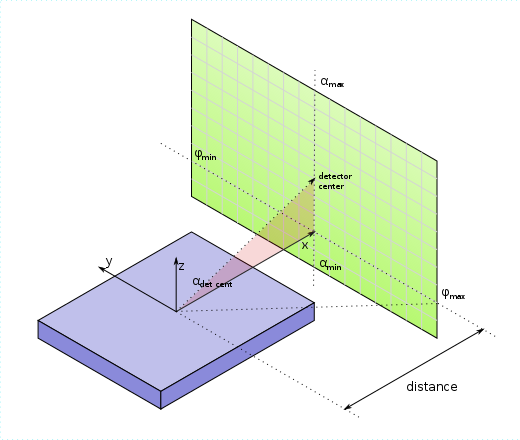
\includegraphics[width=.5\textwidth]{fig/drawing/experimental_geometry.png}
\end{center}
\caption{Experimental geometry with a twodimensional pixel detector.}
\label{FexpGeom}
\end{figure}

To conclude this chapter on the foundations of small-angle scattering,
we shall derive the geometric factors
that allow us to convert differential cross sections into detector counts.
We shall also discuss how to present data on a physically meaningful scale.

%===============================================================================
\subsection{Coordinate transform}
%===============================================================================

We assume that scattered radiation is detected in a flat,
two-dimensional detector
that generates histograms on a rectangular grid,
consisting of $n\cdot m$ pixels of constant width and height,
as sketched in Fig.~\ref{FexpGeom}.
This figure also shows the coordinate system
\index{Conventions|see {Coordinate system}}%
\index{Coordinate system}%
according to unanimous GISAS convention,
with $z$ normal to the sample plane,
and with the incident beam in the $xz$ plane.
The origin is at the sample position;
more precisely, it is for $x$ and $y$ at the center of the sample,
and for $z$ at the sample surface.
We suppose that the detector is mounted perpendicular to the $x$ axis
at a distance $L$ from the sample position.
%the $x$ axis intersects the detector plane at $(L,y_\tc,z_\tc)$.
The real-space coordinate at the center of pixel $(i,j)$ is $(L,y_i,z_i)$.
Each pixel has a width~$\Delta y$ and a height~$\Delta z$.
\index{Detector!pixel coordinate}%
\index{Pixel|see {Detector}}%

Since the differential scattering cross section (\ref{Exsectiondef})
is given with respect to a solid-angle element $\d\Omega$,
we need to express scattered wavevector $\k_\tf$ in spherical coordinates,
using the horizontal azimuth angle~$\phi_\tf$
and the vertical glancing angle $\alpha_\tf$.
The projection of $(\alpha_\tf,\phi_\tf)$ into
the detector plane~$(y,z)$ is known as the \E{gnomonic projection}.
\index{Gnomonic projection}%
\index{Projection!wave vector to pixel coordinate}%
From elementary trigonometry one finds
\begin{equation}\label{Eyzdet}
  \begin{array}{lcl}
  y &=& L \tan\phi_\tf,\\
  z &=& (L/ \cos\phi_\tf) \tan\alpha_\tf.
  \end{array}
\end{equation}
Fig.~\ref{Fconstalphi} shows lines of equal $\alpha_\tf$,~$\phi_\tf$
in the detector plane.

\begin{figure}[t]
\begin{center}
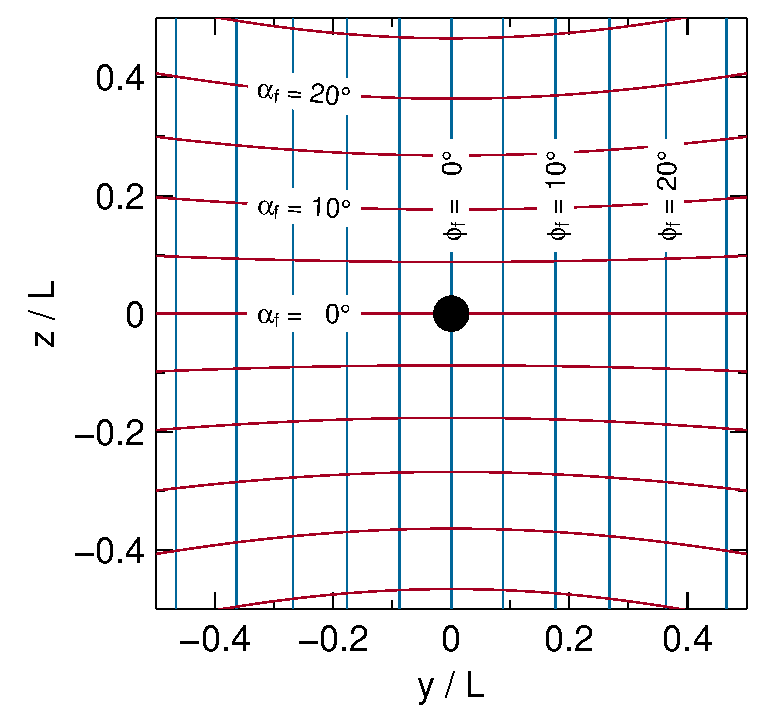
\includegraphics[width=.47\textwidth]{fig/drawing/SAS_const_alphi.ps}
\end{center}
\caption{Lines of constant $\alpha_\tf$ (red) or $\phi_\tf$ (blue)
in the detector plane,
for a planar detector at distance~$L$ from the sample.
The black dot indicates the beamstop location for 
the central incident beam ($\hat\k_\ti = \hat x$).}
\label{Fconstalphi}
\end{figure}

To determine the scattering vector $\q_{ij}$ 
that corresponds to a pixel $(i,j)$,
we need to express the outgoing wavevector~$\k_\tf$ as function of $y$ and~$z$.
This can be done either by inverting (\ref{Eyzdet})
and inserting the so obtained $\alpha_\tf(y,z)$ and $\phi_\tf(y)$ in
\begin{equation}\label{Ekf_by_angle}
  \k_\tf=K\left(\begin{array}{c}
   \cos\alpha_\tf\cos\phi_\tf\\
   \cos\alpha_\tf\sin\phi_\tf\\
   \sin\alpha_\tf\end{array}\right),
\end{equation}
or much more directly by using geometric similarity in Cartesian coordinates.
The result is rather simple:
\Emph{
\begin{equation}\label{Ekf_by_pixel}
  \k_\tf=\frac{K}{\sqrt{L^2+y^2+z^2}}\left(\begin{array}{c}
   L\\
   y\\
   z\end{array}\right).
\end{equation}
\vspace*{-5pt}}
The wavevector $\q_{ij}$ can then be determined through the following steps:
\begin{equation}\label{Eqalgo}
  \begin{array}{cl}
      (i,j)&\\
      \downarrow&\mbox{affine-linear relations}\\
      (y,z)\\
      \downarrow&\mbox{use (\protect\ref{Ekf_by_pixel})}\\
      \k_\tf&\\
      \downarrow&\mbox{use (\protect\ref{Eq})}\\
      \q&\\
  \end{array}
\end{equation}
where the first step is mathematically trivial,
but requires an experimental calibration of the origin of the $(x,y)$ scale.

The solid angle under which a detector pixel
is illuminated from the sample is in linear approximation
\begin{equation}
  \Delta\Omega
  = \cos\alpha_\tf\:\Delta\alpha_\tf\,\Delta\phi_\tf
  = \cos\alpha_\tf
    \left|\frac{\partial(\alpha_\tf,\phi_\tf)}{\partial(y,z)}\right|
    \Delta y \,\Delta z
  = \cos^3\!\alpha_\tf\, \cos^3\!\phi_\tf\: \frac{\Delta y \,\Delta z}{L^2}.
\end{equation}
\index{Detector!illumination angle correction factor}%
\index{Illumination!detector}%
Altogether,
the expected count rate in detector pixel $(i,j)$ is proportional to
\begin{equation}\label{EItrafo_cos}
  I_{ij} = \cos^3\!\alpha_\tf\, \cos^3\!\phi_\tf\:
          \frac{\partial\sigma}{\partial\Omega}(\q_{ij}),
\end{equation}
where we have omitted constant factors $L^{-2}$, $\Delta y$ and $\Delta z$.
Using pixel coordinates instead of angles, this can be rewritten as
\Emph{%
\begin{equation}\label{EItrafo_pix}
  I_{ij} = \left( 1+\frac{y^2+z^2}{L^2}\right)^{-3/2}
          \frac{\partial\sigma}{\partial\Omega}\bigl(\q_{ij}(y,z)\bigr).
\end{equation}
\vspace*{-2pt}}
%(usually as the centre between the transmitted
%and the specularly reflected beam spot).

%===============================================================================
\subsection{Data representation}
%===============================================================================

\begin{figure}[t]
\begin{center}
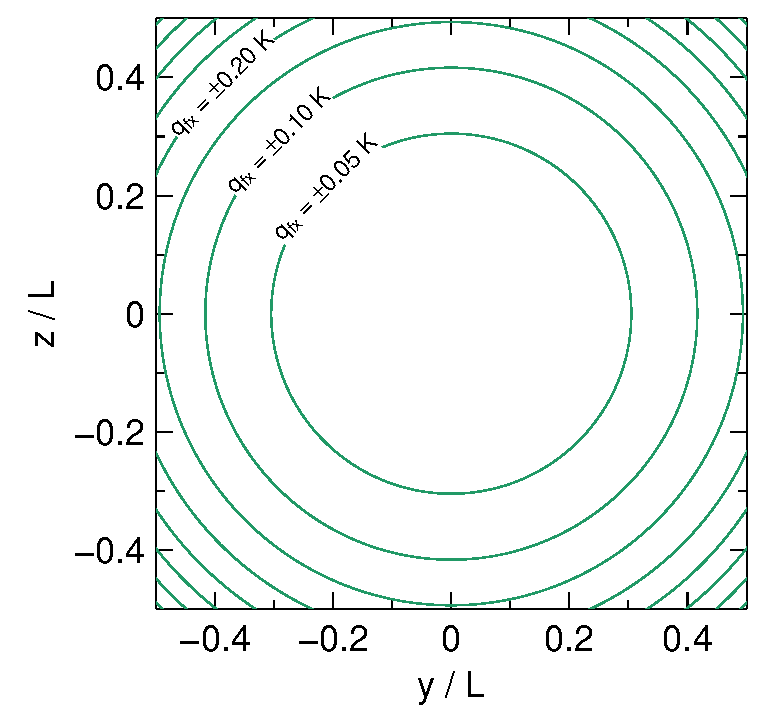
\includegraphics[width=.47\textwidth]{fig/drawing/SAS_const_q_x.ps}
\hfill
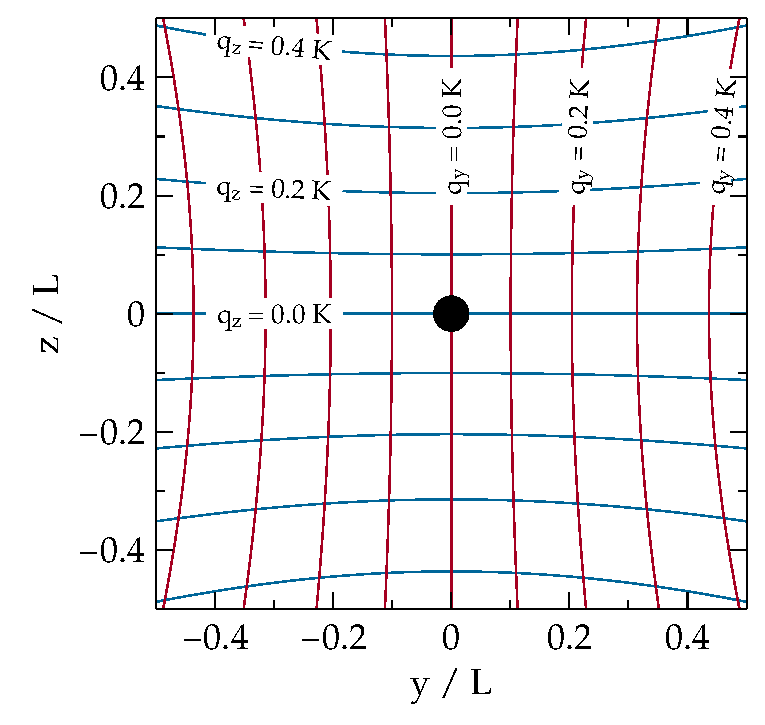
\includegraphics[width=.47\textwidth]{fig/drawing/SAS_const_q_yz.ps}
\end{center}
\caption{Lines of constant $q_x$ (left), $q_y$ or $q_z$ (right),
in units of the incident wavenumber $K=2\pi/\lambda$,
for a planar detector and a central incident beam as in Fig.~\protect\ref{Fconstalphi}.}
\label{Fconstq}
\end{figure}

The transform (\ref{Eqalgo}) between pixel coordinates $y$,~$z$
and physical scattering vector components $q_y$, $q_z$
is nonlinear, due to the square-root term in the denominator of~(\ref{Ekf_by_pixel}).
For $y,z\ll L$, however, nonlinear terms loose importance.
To emphasize nonlinearities,
Figs.~\ref{Fconstalphi}--\ref{Fconstp}
show the rather extreme conditions at scattering angles of up to 45$^\circ$,
which are unusually large angles by the standards of SAS or GISAS.
In most experimental situations,
angles, and therefore nonlinearities, are considerably smaller.

\begin{figure}[t]
\begin{center}
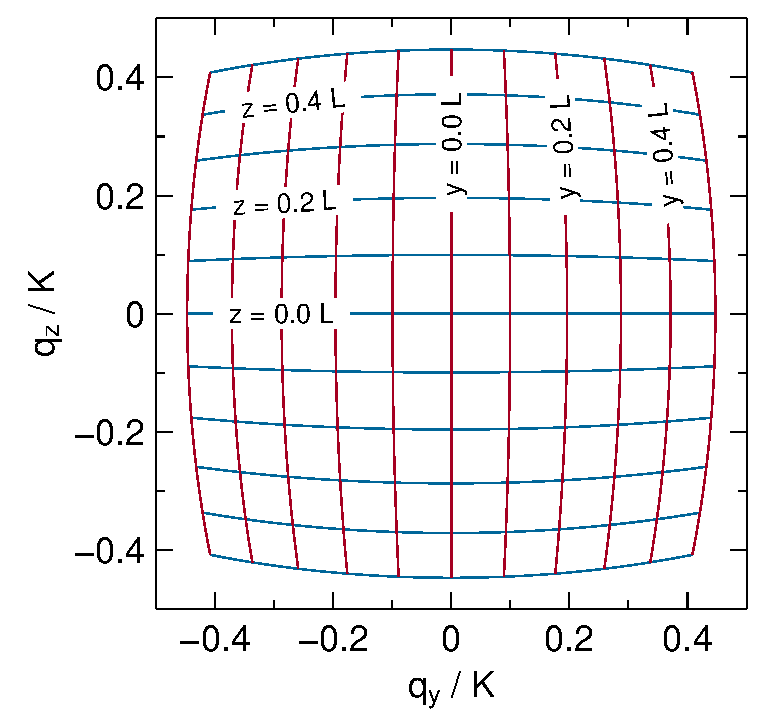
\includegraphics[width=.47\textwidth]{fig/drawing/SAS_const_p_yz.ps}
\end{center}
\caption{The outer contour of the blue and red grid
shows the border of a square detector image 
after transformation into the physical coordinates $q_y$,~$q_z$.
The blue and red curves correspond to horizontal and vertical lines in the detector.}
\label{Fconstp}
\end{figure}

The left detector frame in Fig.~\ref{Fconstq}
shows circles of constant values of $\pm q_x$.
For given steps in $q_x$, the distance between adjacent circles
increases towards the detector center.
From (\ref{Eq}) and (\ref{Ekf_by_pixel}),
one finds asymptotically for $y,z\to L$
that $q_x$ goes with the square of the two other components of the scattering vector,
\begin{equation}\label{Eqxasy}
  \frac{q_x}{K}
  \doteq \frac{y^2+z^2}{2 L^2} 
  \doteq \frac{q_y^2 + q_z^2}{2K^2}.
\end{equation}
Therefore, under typical small angle conditions $y,z\to L$
the dependence of the scattering signal on $q_x$ is unimportant:
one basically measures $\chi(\q)\simeq \chi(0,q_y,q_z)$.

\Work{Show consequences of $q_x$ for box example.}

As anticipated in (\ref{Eqxasy}),
the other two components of $\q$ are in first order linear in the pixel coordinates,
\begin{equation}
  \frac{q_y}{K}=\frac{y}{L}\left(1-\frac{y^2+z^2}{2L^2}+\ldots\right),
\end{equation}
and similarly for~$q_z$.
The nonlinear correction terms lead to the pincushion distortion 
shown in the right detector frame in Fig.~\ref{Fconstq}.
\index{Distortion!of $q_x$, $q_y$ grid in detector plane}%
\index{Detector!distortion of $q_x$, $q_y$ grid}%
\index{Pincushion distortion}%

Since pixel coordinates are meaningful only
with respect to a specific experimental setup,
users may wish to transform detector images
towards the physical coordinates $q_y$ and~$q_z$.
As shown in Fig.~\ref{Fconstp},
this would yield a barrel-shaped ilumminated area
in the $q_y$,~$q_z$~plane.

\Note{\indent Transforming detector images 
  from pixel coordinates into the $q_y$,~$q_z$~plane is not implemented in \BornAgain,
  and not on our agenda.
  We would, however, like to hear about use cases.}

\Emph{\indent When simulating and fitting experimental data with \BornAgain,
detector images remain unchanged.
All work is done in terms of reduced pixel coordinates $y/L$ and~$z/L$.
Corrections are applied to the simulated, not to the measured data.}

\Work{\indent \ldots show how to plot $q$ grid on top of detector image \ldots}

%Tradition wants that raw data be \E{treated} or \E{reduced}
%before they are \E{analyzed}.
%In our case, raw data reduction would comprise 
%the transform (\ref{Eqalgo}) of pixel coordinates into scattering vectors,
%and the accompanying renormalization (\ref{EItrafo}) of pixel counts.

%===============================================================================
\subsection{Symmetry}
%===============================================================================

\Work{to write ... and to continue in other chapters}

\index{Small-angle scattering|)}%

%%%%%%%%%%%%%%%%%%%%%%%%%%%%%%%%%%%%%%%%%%%%%%%%%%%%%%%%%%%%%%%%%%%%%%%%%%%%%%%%
%%
%%   BornAgain User Manual
%%
%%   homepage:   http://www.bornagainproject.org
%%
%%   copyright:  Forschungszentrum Jülich GmbH 2015
%%
%%   license:    Creative Commons CC-BY-SA
%%   
%%   authors:    Scientific Computing Group at MLZ Garching
%%               C. Durniak, M. Ganeva, G. Pospelov, W. Van Herck, J. Wuttke
%%
%%%%%%%%%%%%%%%%%%%%%%%%%%%%%%%%%%%%%%%%%%%%%%%%%%%%%%%%%%%%%%%%%%%%%%%%%%%%%%%%

\chapter
%{GISAS and the DWBA}
{Grazing-incidence scattering and the distorted wave Born approximation}
  \label{SGisas}
\chaptermark{GISAS and the DWBA}

In this chapter,
introduce grazing-incidence small-angle scattering
and its standard theoretical treatment by means of the
distorted wave Born approximation (Sect.~\ref{Sdwba}).
We also discuss the limits of coherent superposition (Sect.~\ref{Scoherlen}),
and the treatment of absorption (Sect.~\ref{Sabsorption}).


%%%%%%%%%%%%%%%%%%%%%%%%%%%%%%%%%%%%%%%%%%%%%%%%%%%%%%%%%%%%%%%%%%%%%%%%%%%%%%%%
\section{Scattering under grazing incidence}\label{Sdwba}
%%%%%%%%%%%%%%%%%%%%%%%%%%%%%%%%%%%%%%%%%%%%%%%%%%%%%%%%%%%%%%%%%%%%%%%%%%%%%%%%

%===============================================================================
\subsection[Wave propagation in $2+1$ dimensions]{Wave propagation in $\v{2+1}$ dimensions}\label{Swave21}
%===============================================================================

\begin{figure}[tb]
  \centering
    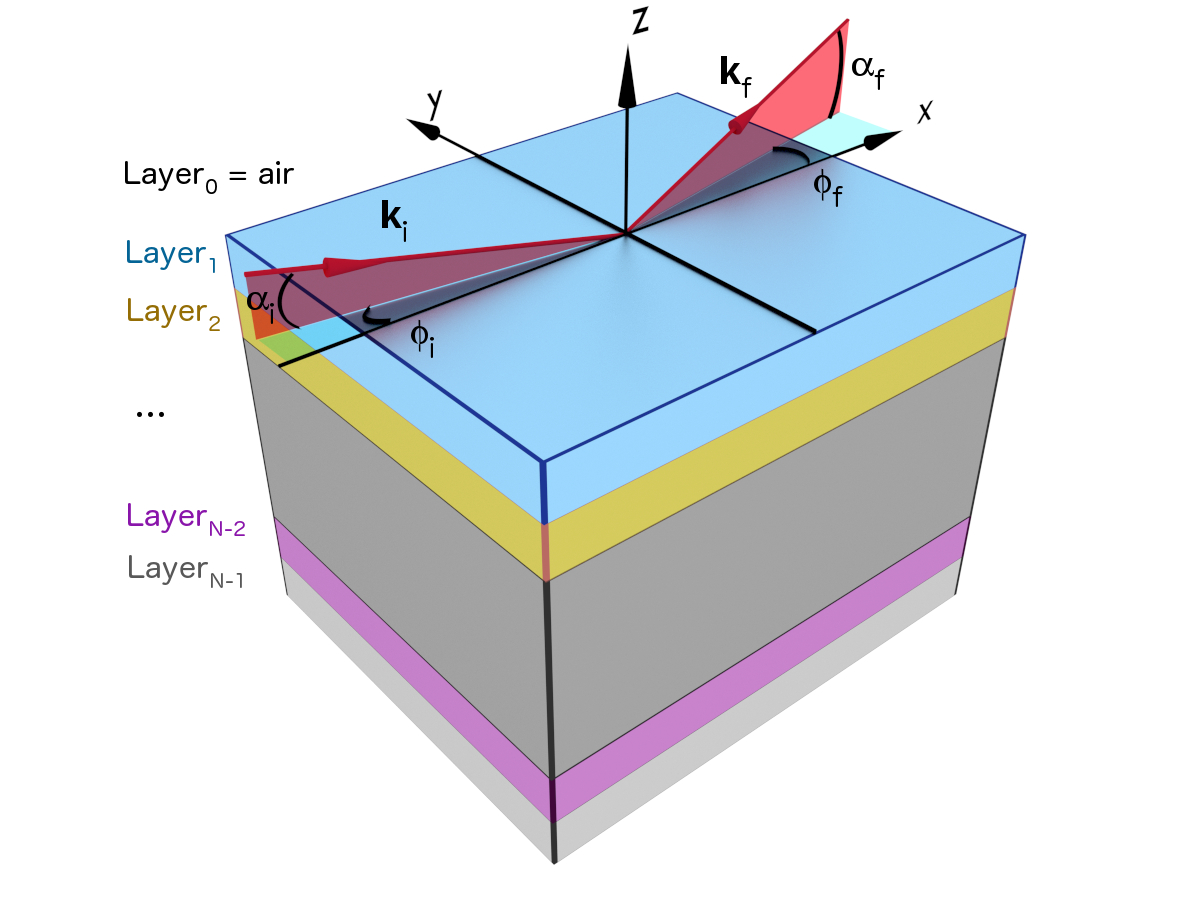
\includegraphics[clip=, width=120mm]{fig/drawing/setup_multilayer.jpg}
  \caption[Conventional GISAS scattering geometry.]{Geometric conventions
  in GISAS scattering comprise a Cartesian coordinate system
  and a set of angles.
  The coordinate system has a $z$ axis normal to the sample plane,
  and pointing into the halfspace where the beam comes from.
  The $x$ axis usually points along the incident beam,
  projected onto the sample plane.
  Incident and final plane waves are characterized
  by wavevectors $\k_\ti$, $\k_\tf$;
  the angle $\alpha_\ti$ is the incident glancing angle;
  $\phi_\ti$ is usually zero, unless used to describe a sample rotation;
  $\alpha_\tf$ is the exit angle with respect to the sample's surface;
  and $\phi_\tf$ is the scattering angle with respect to the scattering plane.
\nomenclature[1α024 2i000]{$\alpha_\ti$}{Glancing angle of the incident beam}
\nomenclature[1α024 2f000]{$\alpha_\tf$}{Glancing angle of the detected beam}
\nomenclature[1φ024 2i000]{$\phi_\ti$}{Angle between the incident beam, projected into the sample plane, and the $x$ axis}%
\nomenclature[1φ024 2f000]{$\phi_\tf$}{Angle between the detected beam, projected into the sample plane, and the $x$ axis}%
\nomenclature[2x020]{$x$}{Horizontal coordinate, usually chosen along the incoming beam projection}%
\nomenclature[2y020]{$y$}{Horizontal oordinate, chosen normal to $z$ and $x$}%
  The numbered layers illustrate a multilayer system as dicussed
  in Sect.~\ref{sec:Multilayers}.
  }
  \label{fig:expgeom}
\end{figure}

Reflectometry and grazing-incidence scattering
are designed for the investigation of surfaces, interfaces, and thin layers,
or most generically:
samples with a $2+1$ dimensional structure
that are on average translationally invariant in $x$ and $y$ direction,
but structured in $z$ direction.
By convention,
we designate the \E{sample plane} ($xy$) as \E{horizontal},
\index{Sample plane}%
\index{Horizontal plane}%
and the \E{sample normal} ($z$) as \E{vertical},
\index{Sample normal}%
\index{Vertical direction}%
\index{Conventions|see {Horizontal and Vertical}}%
even if this does not correspond to the actual experimental geometry.\footnote
{In many reflectometers,
 the scattering plane and the sample normal are horizontal in laboratory space.}
The $z$ axis points upwards, hence out of the sample towards the
vacuum (or air) halfspace where the incident radiation comes from,
as illustrated in Fig.~\ref{fig:expgeom}.
% TODO: add figure

Vertical modulations of the refractive index $n(\r)$
cause refraction and reflection of an incident plane wave.
\index{Glancing angle}%
\index{Refraction}%
\index{Reflection}%
For small glancing angles,
these distortions can be arbitrary large,
up to the limiting case of total reflection,
even though $1-n$ is only of the order $10^{-5}$ or smaller.
Such zeroth-order effects cannot be accounted for
by perturbative scattering theory.
Instead, we need to deal with refraction and reflection
at the level of the wave propagation equation.
We move the vertical variations of the squared refractive index
to the left-hand side of the Schrödinger equation~(\ref{EnSchrodi}),
\begin{equation}\label{EHelmholtzGraded}
  \left\{\Nabla^2+K^2\nz(z)\right\}\psi(\r)
  = 4\pi \chi(\r) \psi(\r),
\end{equation}
\nomenclature[2z020]{$z$}{Vertical coordinate, along the sample normal)}%
\nomenclature[2n030 2z020]{$\nz(z)$}{Refractive index, horizontally averaged}%
where the overline indicates an horizontal average.
Deviating from (\ref{EChiDef}),
the perturbation has been redefined as
\begin{equation}\label{EChiGraded}
  \chi(\r) \coloneqq  \frac{K^2}{4\pi}\left(\nz(z)-n^2(\r)\right),
\end{equation}
which only accounts for horizontal fluctuations of the refractive index.
Wave propagation,
unperturbed by~$\chi$, but including refraction and reflection effects,
obeys the homogeneous equation
\begin{equation}\label{EHelmholtzGradedHomog}
  \left\{\Nabla^2+K^2\nz(z)\right\}\psi(\r) = 0.
\end{equation}
It is solved for the horizontal coordinate~$\r_\parallel$
by the factorization ansatz
\Emph{
\begin{equation}\label{Ekpar}
\psi(\r) = \e^{i \k_\parallel\r_\parallel} \phi(z).
\end{equation}\vspace*{-10pt}
}
\nomenclature[2k041\parallel]{$\k_\parallel$}{Projection of $\k$ onto the sample plane}%
\nomenclature[1φ020 0z020]{$\phi(z)$}{$z$-dependent factor of $\psi(\r)$}%
The horizontal wavevector $\k_\parallel$ remains constant
as initialized by the incoming beam.
The vertical wavefunction must fulfill
\Emph{
\begin{equation}\label{Ewavez}
\left\{\partial_z^2 + K^2\nz(z) - k_\parallel^2 \right\} \phi(z) = 0.
\end{equation}\vspace*{-10pt}
}
When an incident plane wave,
travelling downwards with
$\phi(z)=\e^{-ik_\perp z}$,
\nomenclature[2k021\perp]{$k_\perp$}{Component of $\k$ along the sample normal}%
impinges on a sample with $\nz(z)\ne 1$,
then the wave is partly reflected ($-k_\perp$ reversed into $+k_\perp$)
and partly refracted
($k_\perp$ changing while $\k_\parallel$ stays constant,
resulting in a change of glancing angle).
Similarly, reflection and refraction occur
whenever $\nz(z)$ varies within the sample.
As a result, at any $z$ within the zone where $\nz(z)$ varies,
the vertical wavefunction $\phi(z)$ is composed of a
downward travelling component $\phi^-(z)$
and an upward travelling component $\phi^+(z)$.

For a graded refractive index
\index{Refractive index!graded}%
$\nz$ that is a smooth function of~$z$,
the differential equation~(\ref{Ewavez}) is best solved
using the WKB method.\footnote
{Also called \E{semiclassical approximation} or
\E{phase integral method},
%originally developed
%by Liouville (1837), Green (1837), Lord Rayleigh (1912), and Jeffreys (1923),
named after Wentzel (1926), Kramers (1926), Brillouin (1926).
See any textbook on quantum mechanics.}
\index{WKB method}%
\index{Semiclassical approximation|see {WKB method}}%
\index{Phase integral method|see {WKB method}}%
If otherwise $\nz(z)$ is discontinuous at some interface $z=z_j$,
then the limiting values of $\phi^-(z)$ and $\phi^+(z)$
on approaching $z_j$ from above or below
are connected to each other through Fresnel's
transmission and reflection coefficients.
\index{Fresnel coefficients}%
This applies in particular to multilayer systems,
discussed in chapter~\ref{sec:Multilayers}.

%===============================================================================
\subsection{Distorted-wave Born approximation (DWBA)}\label{SDWBA}
%===============================================================================

\index{Distorted-wave Born approximation|(}%
\index{DWBA|see {Distorted-wave Born approximation}}%

The standard form of the Born approximation,
as presented in Sect.~\ref{SBorn},
combines an approximation scheme
(computing (\ref{EPsiFormal}) by iteration)
with an assumption (the incident field is a plane wave)
and an analytic result
(in far-field approximation,
the Green function of the Helmholtz equation is a plane wave
with respect to the locus of scattering).
These three elements must not necessarily go together.
We can apply the very same approximation scheme,
even if the incident field is not a plane wave,
but a \E{distorted wave},
namely a superposition of downwards and upwards travelling plane waves,
as derived in the previous section.
This is the core idea
of the \E{distorted-wave Born approximation} (DWBA).\footnote
{The distorted-wave Born approximation
was originally devised by Massey and Mott (ca 1933)
for collisions of charged particles.}
% Schiff (^3 1968, p 327) cites
% Mott, Massey, The Theory of Atomic Collisions, p 100, Oxford 1933;
% There are also several papers by Massey and Mott from about 1933.

To carry out this idea, we need to determine the Green function~$G$.
\index{Green function!vertically structured material}%
In Sect.~\ref{SBorn} we did so quite specifically
for a homogeneous material.
Computing~$G$ in closed form for a more generic wave equation
like~(\ref{EHelmholtzGradedHomog}) is far more difficult,
if not outright impossible.
Fortunately, this computation is not necessary,
and would be but wasted effort:
We do not need the full solution~$G(\r,\r')$,
but only its asymptotic far-field value $G(\rD,\r')$
at a detector position $\rD$.
\nomenclature[2r041 2d100]{$\rD$}{Position of the detector}%
Thanks to a \E{source-detector reciprocity theorem}~(\ref{Ereci})
\index{Reciprocity}%
proven in Appendix~\ref{Sreci1},
we can compute this value
as
\begin{equation}\label{EreciDup}
  G(\rD,\r) = B(\r,\rD),
\end{equation}
\nomenclature[2b030 2r040 2r041]{$B(\r,\r')$}{Green function, adjoint of $G$}%
where~$B$ is the \E{adjoint Green function}
that describes backward propagation from $\rD$ into the sample.

Outside the sample,
$B$ obeys the Helmholtz equation
with isolated inhomogeneity (\ref{EHelmholtzForGreen}),
and therefore has the far-field expansion~(\ref{EGreenFar}),
\index{Far-field approximation}%
\begin{equation}\label{EBFar}
  B_\text{far}(\r,\rD)
  =\frac{\e^{iKr_\text{D}}}{4\pi r_\text{D}}\e^{-i\k_\tf \r}.
\end{equation}
When this backward propagating plane waves impinges on the sample,
it undergoes reflection and refraction in exactly the same way as
the incident plane wave $\e^{i\k_\ti\r}$.
Therefore,
 (\ref{EBFar}) admits a generalization that also holds inside the sample:
\begin{equation}\label{EBFull}
  B_\text{far}(\r,\rD)
  = \frac{\e^{iKr_\text{D}}}{4\pi r_\text{D}}\psi^*_\tf(\r).
\end{equation}
Applying now the reciprocity theorem (\ref{EreciDup}),
we obtain
\begin{equation}\label{EGreenFarDWBA}
  G_\text{far}(\r,\r')
  = \frac{\e^{iKr}}{4\pi r}\psi^*_\tf(\r')
\end{equation}
which agrees literally with (\ref{EGreenFar}),
though $\psi_\tf$ is not any longer a plane wave.
Accordingly,
the scattered far-field is still given by (\ref{EsandwichC}),
and the differential cross section by (\ref{Exsection}).
We only need to redetermine the matrix element
$\bra \psi_\ti|\chi|\psi_\tf\ket$,
which no longer has the plane-wave form~(\ref{Echiq}).

Since both the incident
and the scattered distorted wavefunction
are composed of downward and upward propagating waves,
\begin{equation}\label{Epsipm}
  \psi_w(\r)
  = \psi^-_w(\r) + \psi^+_w(\r)
  \quad\text{with}\quad
  w=\ti,\tf,
\end{equation}
\nomenclature[2w010]{$w$}{An index that can take the values i (incident)
or f (final)}%
the matrix element can be expanded into four terms,
\begin{equation}\label{Edwba4}
  \bra \psi_\ti|\chi|\psi_\tf\ket
  = \bra \psi^-_\ti|\chi|\psi^-_\tf\ket
  + \bra \psi^-_\ti|\chi|\psi^+_\tf\ket
  + \bra \psi^+_\ti|\chi|\psi^-_\tf\ket
  + \bra \psi^+_\ti|\chi|\psi^+_\tf\ket,
\end{equation}
\nomenclature[1ψ041 0\pm 2r040]{$\psi^\pm(\r)$}{Upward ($+$) or downward ($-$) propagating component of $\psi(\r)$}%
\nomenclature[0\pm]{$\pm$}{Upward ($+$) or downward ($-$) propagating}%
or in an obvious shorthand notation
\Emph{%
\begin{equation}\label{Edwba}
  \bra \psi_\ti|\chi|\psi_\tf\ket
  = \sum_{\pm_\ti} \sum_{\pm_\tf}
    \bra \psi^\pm_\ti|\chi|\psi^\pm_\tf\ket.
\end{equation}%
\vspace*{-5pt}}
This equation contains the essence of
the distorted-wave Born approximation
for small-angle scattering under grazing incidence,
and is the base for all scattering models implemented in \BornAgain.
Since $\bra \psi_\ti|\chi|\psi_\tf\ket$
appears as a squared modulus
in the differential cross section~(\ref{Exsection}),
the four terms of (\ref{Edwba}) can interfere with each other,
which adds to the complexity of GISAS patterns.

\index{Distorted-wave Born approximation|)}%


%%%%%%%%%%%%%%%%%%%%%%%%%%%%%%%%%%%%%%%%%%%%%%%%%%%%%%%%%%%%%%%%%%%%%%%%%%%%%%%%
\section{Coherence length}\label{Scoherlen}
%%%%%%%%%%%%%%%%%%%%%%%%%%%%%%%%%%%%%%%%%%%%%%%%%%%%%%%%%%%%%%%%%%%%%%%%%%%%%%%%

\index{Coherence length|(}%
The matrix elements $\bra \psi^\pm_\ti|\chi|\psi^\pm_\tf\ket$
are given by three-dimensional integrals~(\ref{Etrama}),
\begin{equation}\label{Etrama3}
  \bra \psi_\ti^\pm|\chi|\psi_\tf^\pm\ket
  \coloneqq  \int\!\d^3r\, \psi^{\pm*}_\ti(\r)\chi(\r)\psi^\pm_\tf(\r).
\end{equation}
The integration domain is effectively limited to a finite $z$ interval,
where $\chi(\r)$ is horizontally modulated.
On the other hand, the horizontal integration domain is infinite
within our formalism,
which is of course an idealization.
Obviously, physical integration limits are imposed by the finite
\E{illuminated sample area}.\footnote
{For a given instrument setup,
the incoming beam illuminates a finite area~$A_\ti$ in the sample plane,
and similarly, scattered radiation is only detected if it originates
from an area~$A_\tf$ that can be determined
by tracing back rays from the detector
to their intersection with the sample plane.
In a well aligned instrument, $A_\ti$ and $A_\tf$ are nearly the same.
Let $A_\text{beam}\coloneqq A_\ti\cap A_\tf$.
In a well aligned experiment,
$A_\text{beam}$ is equal to or a subset of $A_\text{sample}$
(if $A_\ti$ or $A_\tf$ are larger than $A_\text{sample}$,
collimation slits should be narrowed
lest useless rays cause avoidable noise).
Anyhow, the horizontal integration domain
is limited to the \E{illuminated sample area} (``beam footprint'')
$A_{xy}\coloneqq A_\text{sample}\cap A_\text{beam}$.}
\index{Sample area}%
\index{Illumination!beam footprint on sample}%
\index{Beam footprint}%
Another limitation comes from the finite \E{coherence length}
of the instrumental setup,
which usually is much shorter than the sample width and length
%This is of importance in neutron scattering
%where typical sample dimensions of 1\ldots10~mm
%are much larger than the relevant coherence length,
%which is of the order 10\ldots100~$\upmu$m 
\cite{HaPR10,MaMM14}.\footnote
{These two references also make clear that
  the theoretical description and the experimental determination of
  coherence lengths are difficult problems and subject of ongoing research.}

While each single neutron is described by a wavefunction
that allows for \E{coherent} superposition of
different contributions to the scattered wavefunction,
the final detector statistics
\index{Detector statistics}%
is given by an \E{incoherent} sum
over the differential cross sections of individual neutrons.
The finite \E{resolution}
\index{Resolution|(}%
of an experimental setup is in part due to the fact that
different neutrons have different wavenumbers,
originate\footnote
{It is reasonable to take the last collision in the moderator
  as the \E{origin} of a neutron ray,
  since collisions between neutrons and hydrogen nuclei bound in
  disordered matter lead to almost perfect decoherence.}
at different points in the moderator,
and are detected at slightly different points within one detector pixel.
This can be modeled by computing expected scattering intensities as
averages over different neutrons with 
$K$, $\v{\hat k}_\ti$, and $\v{\hat k}_\tf$ drawn at random
from appropriate distributions,
as described in Sect.~\ref{Sresolution}.

However, this is not the full story.
In the above introduction to the Born approximation
we have made the standard assumption
that an incoming neutron can be described by a plane wave
$\psi_\ti=\e^{i\k_\ti\r}$.
The wavefunction $\psi_\tf$ traced back from the detector is also
approximated by a plane wave.
In the DWBA we allow these waves to be distorted within the sample,
but when impinging on the sample they still are plane.
A plane wave obviously is an idealized concept,
since it has infinite lateral extension.
The \E{transverse coherence length} indicates the scale
beyond which this approximation becomes invalid.
At larger scales, the wave fronts appear randomly distorted.
Physical causes of these distortions include
reflections in the neutron guide,
diffraction by guide windows and other slits,
and diffraction by imperfect monochromator crystals.
Of course the distorted wave still admits a Fourier decomposition
into plane waves with slightly different wavevectors.
In practice, it is impossible to distinguish this spread of wavevectors
from the incoherent spread described in the previous paragraph.
The instrumental resolution function therefore
accounts for both causes of wavevector distortion.
\index{Resolution|)}%

Usually, therefore, a GISANS image is an incoherent average
over coherent diffraction patterns collected from 
many small subareas of the sample.
Only horizontal sample structures on scales smaller the coherence length
yield interference patterns.
Structure fluctuations on larger scales
produce said incoherent average of different GISANS images.

The crossover from coherent to incoherent scattering is of course
a gradual one.
The coherence length, however defined,
indicates where a certain, somewhat arbitrary degree
of decoherence is reached.
Under these reservations
one defines a \E{coherence spot}
in the cross section of an approximately plane wave
as an area where the coherence is above a certain threshold.
Unless the wave has been prepared in a highly anisotropic guide and slit system,
this spot is about circular.
Under grazing incidence conditions however,
the projection of this spot onto the sample surface
yields a very elongated ellipse.
Therefore, the coherence length is much larger in $x$ than
in $y$ or $z$ direction.\footnote
{This has nothing to do with the distinction of
  \E{transverse} and \E{longitudinal} coherence length.
  Longitudinal coherence has to do with wavelength stability
  and is of no importance for elastic scattering.
  We are talking here about \E{horizontal} and \E{vertical}
  projections of the \E{transverse} coherence length.}

\Note{\indent Unless otherwise said, \BornAgain\ simulates
  \E{coherent} diffraction patterns obtained by
  the linear superposition of scattered waves.
  To simulate an \E{incoherent} mixture of diffraction patterns,
  the most generic solution is a script with an outer loop
  that averages over several coherent computations with
  appropriately distributed parameters.}

% TODO: more about implementation !

\index{Coherence length|)}%

%%%%%%%%%%%%%%%%%%%%%%%%%%%%%%%%%%%%%%%%%%%%%%%%%%%%%%%%%%%%%%%%%%%%%%%%%%%%%%%%
\section{Absorption}\label{Sabsorption}
%%%%%%%%%%%%%%%%%%%%%%%%%%%%%%%%%%%%%%%%%%%%%%%%%%%%%%%%%%%%%%%%%%%%%%%%%%%%%%%%

\index{Absorption|(}%
\index{Refractive index!sign convention}%
The complex refractive index of a given material
shall be written as
\begin{equation}\label{Endb1}
  n\doteq 1-\delta +i\beta,  
\end{equation}
\nomenclature[1δ020]{$\delta$}{Small parameter in the refractive index
   $n=1-\delta +i\beta$}%
\nomenclature[1β020]{$\beta$}{Imaginary part of the refractive index}%
introducing two small real parameters $\delta, \beta$.
However, 
in our derivations, which are all rooted in~(\ref{EnSchrodi}),
$n$ only appears as $n^2$. 
Therefore, we actually \E{define}
\begin{equation}\label{Endb2}
  n^2\coloneqq 1-2\delta+2i\beta,
\end{equation}
and read (\ref{Endb1}) as an excellent approximation.

While the real part of $n$ is responsible for refraction, reflection,
and scattering,
the imaginary part describes absorption
and leads to a damping of propagating waves.
The plus sign in front of the imaginary part is a consequence of
the quantum-mechanical sign convention;
in the X-ray crystallography convention it would be a minus sign.
\index{Sign convention}%

The factorization ansatz (\ref{Ekpar}) leaves us some freedom
how to deal with an imaginary part of~$n$.
We \E{choose} that horizontal wavevectors~$\k_\parallel$
shall always be real.
The damping then appears in the vertical wavefunction~$\phi(z)$
that is governed by the complex wave equation (\ref{Ewavez}).

\index{Absorption|)}%

%%%%%%%%%%%%%%%%%%%%%%%%%%%%%%%%%%%%%%%%%%%%%%%%%%%%%%%%%%%%%%%%%%%%%%%%%%%%%%%%
%%
%%   BornAgain User Manual
%%
%%   homepage:   http://www.bornagainproject.org
%%
%%   copyright:  Forschungszentrum Jülich GmbH 2015
%%
%%   license:    Creative Commons CC-BY-SA
%%   
%%   authors:    Scientific Computing Group at MLZ Garching
%%               C. Durniak, M. Ganeva, G. Pospelov, W. Van Herck, J. Wuttke
%%
%%%%%%%%%%%%%%%%%%%%%%%%%%%%%%%%%%%%%%%%%%%%%%%%%%%%%%%%%%%%%%%%%%%%%%%%%%%%%%%%

\chapter{Polarized GISAS}  \label{SPol}

In this chapter,
we generalize our treatment of wave propagation and
grazing-incidence small-angle scattering
to X-rays and polarized neutrons.
We therefore need to study vectorial wave equations,
in contrast to the scalar theory of the previous chapter.

%===============================================================================
\section{X-ray propagation}\label{Sxray}
%===============================================================================
\index{Wave propagation!X-rays}
\index{X-rays!wave propagation}

\MissingSection


%===============================================================================
\section{Polarized neutrons}\label{Snpol}
%===============================================================================

\index{Neutrons!polarized}
\index{Polarization!neutrons}

\MissingSection


%%%%%%%%%%%%%%%%%%%%%%%%%%%%%%%%%%%%%%%%%%%%%%%%%%%%%%%%%%%%%%%%%%%%%%%%%%%%%%%%
%%
%%   BornAgain User Manual
%%
%%   homepage:   http://www.bornagainproject.org
%%
%%   copyright:  Forschungszentrum Jülich GmbH 2015
%%
%%   license:    Creative Commons CC-BY-SA
%%   
%%   authors:    Scientific Computing Group at MLZ Garching
%%               C. Durniak, M. Ganeva, G. Pospelov, W. Van Herck, J. Wuttke
%%
%%%%%%%%%%%%%%%%%%%%%%%%%%%%%%%%%%%%%%%%%%%%%%%%%%%%%%%%%%%%%%%%%%%%%%%%%%%%%%%%


\chapter{DWBA for multilayer systems}  \label{sec:Multilayers}


\index{Multilayer|(}%
\index{Layer structures|see {Multilayer}}

In Sect.~\ref{Sdwba},
we have discussed wave propagation and scattering in 2$+$1 dimensional systems
that are translationally invariant in the horizontal $xy$ plane,
and have a vertical refractive index profile $\nz(z)$.
Here we specialize to layered systems
where $\nz(z)$ is a step function that is constant within one layer.
First, only scalar interactions are considered.
Later, the theory is extended to account for polarization effects.

\Note{\indent By convention,
layers are numbered from top to bottom.
The top vacuum (or air) layer (which extends to $z\to+\infty$) has number~0,
the substrate (extending to $z\to-\infty$) is layer~$N$.}

All layer interfaces are assumed to be perfectly smooth.
For rough interfaces, see Chapter~\ref{sec:Roughness}.

%%%%%%%%%%%%%%%%%%%%%%%%%%%%%%%%%%%%%%%%%%%%%%%%%%%%%%%%%%%%%%%%%%%%%%%%%%%%%%%%
\section{Scalar case}
%%%%%%%%%%%%%%%%%%%%%%%%%%%%%%%%%%%%%%%%%%%%%%%%%%%%%%%%%%%%%%%%%%%%%%%%%%%%%%%%

%===============================================================================
\subsection{Wave propagation and DWBA matrix element}
%===============================================================================

\index{Multilayer!Indexing convention}%

To compute scattering cross sections in DWBA,
we first need to determine the distorted wave functions~$\psi_w(\r)$
for $\r$ inside the sample.
The following derivation holds for the incoming wave ($w=\ti$)
as well as for the back-traced detected wave ($w=\tf$).

We consider wave propagation in one layer~$j$
\nomenclature[2j020]{$j$}{Index of layer in multilayer sample}%
with constant average refractive index $\nz(z)=\nzj$.
A vacuum plane wave, impinging on a layered structure,
is at each interface partly reflected, partly refracted,
so that the wave function inside a material layer
has an upward and a downward propagating component,
as per~(\ref{Epsipm}).
Each component is a plane wave,
\begin{equation}
  \psi^\pm_{wj}(\r)=\e^{i\k^\pm_{\parallel w}\r_\parallel}\phi^\pm_{wj}(z)
\end{equation}
with
\begin{equation}\label{Ephizwj}
  \phi^\pm_{wj}(\r)=A^\pm_{wj}\e^{\pm i\k_{\perp wj}(z-z_j)}.
\end{equation}
\nomenclature[2a123 2w010 2j010 \pm]{$A^\pm_{wj}$}{Amplitude of the plane wave $\phi^\pm_{wj}(\r)$}%
For later convenience,
the phase factor in (\ref{Ephizwj}) includes an offset
given by~$z_j$, the $z$ coordinate at the bottom of layer~$j$.
The amplitudes $A$ are often written with distinct letters
T and~R to designate the transmitted or reflected beam,
\begin{equation}
  T_{wj} := A^-_{wj},\quad
  R_{wj} := A^+_{wj}.
\end{equation}
\nomenclature[2t126 2w020 2j020 0]{$T_{wj}$}{Partial amplitude of $\psi_w(\r)$
  in layer $j$ in downward (transmission) direction, also denoted $A^-_{wj}$}%
\nomenclature[2r126 2w020 2j020 0]{$R_{wj}$}{Partial amplitude of $\psi_w(\r)$
  in layer $j$ in upward (reflection) direction, also denoted $A^+_{wj}$}%
They need to be computed recursively,
as described in the following subsection~\ref{Sacrolay}.

Each plane wave component $\psi^\pm_{wj}(\r)$ has
a three-dimensional wave vector
\begin{equation}\label{Ekpmwj3}
  \k^\pm_{wj}= \k_{\parallel w} \pm k_{\perp wj}\v{\hat z}.
\end{equation}
\nomenclature[2z060]{$\v{\hat z}$}{Unit vector along the sample normal}%
\nomenclature[2k043 2w010 2j010 \pm]{$\k^\pm_{wj}$}{Wave vector of the plane wave $\Psi^\pm_{wj}(\r)$}%
As explained in connection with~(\ref{Ekpar}),
the in-plane wave vector $\k_{\parallel w}$ remains constant
across layer interfaces.
The vertical wavenumber is obtained from (\ref{Ewavez}),
\begin{equation}\label{Ekperpwj}
  k_{\perp wj} = \sqrt{K^2 \nzj - k_{\parallel w}^2}.
\end{equation}
The glancing angle is
\begin{equation}\label{Edef_alpha}
  \alpha_{wj}:=\arctan(k_{\perp wj}/k_{\parallel w}).  
\end{equation}
Equivalently,
\begin{equation}
  k_{\parallel w}=K n_j \cos\alpha_{wj}. 
\end{equation}
Since $k_{\parallel w}$ is constant across layers,
we have
\begin{equation}\label{ESnell}
  n_j \cos\alpha_{wj} = \text{the same for all }j,
\end{equation}
which is Snell's refraction law.
\index{Refraction!Snell's law}
\index{Snell's law}

Since the $\psi^\pm_{wj}$ are plane waves within layer~$j$,
we can at once write down the DWBA transition matrix~(\ref{EtmDWBAsum})
\index{Distorted-wave Born approximation!multilayer}%
\Emph{
\begin{equation}\label{EtmDWBAft}
  \bra \Psi_\tf|\chi|\Psi_\ti\ket
  = \sum_{j} \sum_{\pm_\tf} \sum_{\pm_\ti}
    A^\pm_{\ti j} A^{\pm *}_{\tf j}
     \chi_j(\k^\pm_{\ti j} - \k^\pm_{\tf j})
\end{equation}\vspace*{-5pt}
}
where
\begin{equation}\label{Echij}
  \chi_j(\v{q})
  := \int_{z_j}^{z_{j-1}}\!\d z \int\!\d^2r_\parallel\, \e^{i\v{q}\,\r}\chi(\r)
\end{equation}
\nomenclature[1χ032 2j010 2q040]{$\chi_j(\v{q})$}{Fourier transform of the perturbation potential $\chi(\r)$, evaluated in one sample layer}%
is the Fourier transform
of the perturbative potential~(\ref{EChiGraded}),
restricted to one layer.

%-------------------------------------------------------------------------------
\subsection{Wave propagation across layers}\label{Sacrolay}
%-------------------------------------------------------------------------------

\index{Fresnel coefficients}%
\index{Transmission|see {Fresnel coefficients}}%
\index{Reflection|seealso {Fresnel coefficients}}%

The plane-wave amplitudes $A^\pm_{wj}$ need to be computed recursively
from layer to layer.
Since these computations are identical for incident and final waves,
we omit the subscript~$w$ in the remainder of this section.
At layer interfaces, the optical potential changes discontinuously.
From elementary quantum mechanics we know that
piecewise solutions of the Schrödinger equations must be connected
such that the wave function $\phi(\r)$ and its first derivative
$\Nabla\phi(\r)$ evolve continuously.
This means for the interface
at the \textit{bottom} of layer~$j=0,\ldots,N-1$:%
\begin{equation}\label{Econtcond}
  \begin{array}{lcl}
            \phi_j(z_j)&=&\phi_{j+1}(z_{j+1}+d_{j+1}),\\
            \partial_z\phi_j(z_j)&=&\partial_z\phi_{j+1}(z_{j+1}+d_{j+1}),
  \end{array}
\end{equation}
  where
\begin{equation}
  d_j:=z_{j-1}-z_{j}
\end{equation}
is the thickness of layer~$j$.

We abbreviate
\begin{equation}
  f_j := k_{\perp j}/K = \sqrt{\overline{n_j^2}-(k_\parallel/K)^2}
\end{equation}
and
\begin{equation}
   \delta_j := \e^{iKf_jd_j}.
\end{equation}
For the plane waves (\ref{Ephizwj}),
the continuity conditions~(\ref{Econtcond}) take the form
\begin{equation}\label{Econt2}
  \begin{array}{lclclcl}
  A^+_j &+& A^-_j,
  &=&
  a_{j+1}\delta_{j+1} &+& A^-_{j+1}\delta_{j+1}^*,
  \\
  A^+_j f_j  &-& A^-_j f_j,
  &=&
 a_{j+1}\delta_{j+1} f_{j+1} &-& A^-_{j+1}\delta_{j+1}^* f_{j+1}.
  \end{array}
\end{equation}
After some lines of linear algebra,
we can rewrite this equation system as
\begin{equation}\label{EcMc}
  \left( \begin{array}{c}A^+_j\\A^-_j\end{array} \right)
  = M_{j+1} \left( \begin{array}{c}A^+_{j+1}\\A^-_{j+1}\end{array} \right)
\end{equation}
with the transfer matrix
\begin{equation}
  M_j
   = \frac{1}{2f_{j-1}}
   \left(\begin{array}{cc}
       \delta_j(f_{j-1}+f_j)&\delta_j^*(f_{j-1}-f_j)\\
       \delta_j(f_{j-1}-f_j)&\delta_j^*(f_{j-1}+f_j)
   \end{array}\right).
\end{equation}
To study wave propagation across the entire stack of layers,
we use the combined transfer matrix
\begin{equation}
   M = M_1 \cdots M_N.
\end{equation}
In our scattering setup,
plane-wave amplitudes are subject to two boundary conditions:
In the top layer, $A^-_{w0}=1$ is given by the
incident or back-traced final plane wave.
In the substrate, $A^+_{wN}=0$ because there is no radiation
coming from $z\to-\infty$.
This leaves us with two unkown amplitudes connected by
\begin{equation}
  \left( \begin{array}{c}A^+_0\\1\end{array} \right)
  = M \left( \begin{array}{c}0\\A^-_N\end{array} \right),
\end{equation}
which is solved by
\begin{equation}
  \begin{array}{lcl}
    A^-_N &=& 1/M_{22},\\[.2ex]
    A^+_0 &=& M_{12}/M_{22}.
  \end{array}
\end{equation}
It is a straightforward exercice to verify
that for a single interface between two semi-infinite media,
the reflection and transmission probabilities
agree with Fresnel's result for $s$-polarized light,\footnote
{See any optics textbook, e.~g. Born~\&~Wolf \cite[ch.~1.5.2]{BoWo99}
  or Hecht \cite[ch.~4.6.2]{Hec02}.}
\begin{equation}
  \left| A^+_0\right|^2
  = \left|\frac{f_0-f_1}{f_0+f_1}\right|^2,
  \quad
  \left| A^-_N\right|^2
  = \left| \frac{2f_0}{f_0+f_1}\right|^2.
\end{equation}

\Work{How does the above relate to what is actually computed in BornAgain?
And how to Abeles matrices, Parrat's formalism, Deak's papers?}

%-------------------------------------------------------------------------------
\subsection{Damped waves in absorbing media
  or under total reflection}\label{s:complex}
%-------------------------------------------------------------------------------

In Sect.~\ref{Sabsorption},
we have chosen the horizontal wave vector $\k_{\parallel}$
to be always real and constant.
In contrast, the vertical wave number $k_{\perp j}$,
given by (\ref{Ekperpwj}),
can become imaginary or complex.
If $\overline{n_j^2}$ is real and smaller than~$n_0^2\cos^2\alpha_0$,
then Snell's law of refraction (\ref{ESnell}) cannot be fulfilled,
and the radicand in (\ref{Ekperpwj}) becomes negative
so that $k_{\perp j}$ becomes pure imaginary.
\index{Wave vector!complex}%
If the layer is absorbing,
described by an positive imaginary part of $\overline{n_j^2}$,
then the radicand in (\ref{Ekperpwj}) becomes complex,
and the wave number $k_{\perp j}$ as well.
For complex $k_{\perp j}$,
the theory developed above remains applicable,
except that the geometric interpretation of the wave vectors $\k_\pm$
in Eqs.~(\ref{Edef_alpha}--\ref{ESnell}) is untenable.

Writing
\begin{equation}
  k_\perp = k_\perp' + i k_\perp''
\end{equation}
for a decomposition into a real and an imaginary part,
we find an exponential decay of the plane wave amplitudes
\begin{equation}\label{Ephidamp}
  \left|\phi^\pm_j(z)\right|
  = \e{\mp k_{\perp j}'' z}
\end{equation}
along their propagation direction~$\pm z$.
With an analogous decomposition
of the three-dimensional wave vector (\ref{Ekpmwj3}),
we obtain for the flux, defined as in~(\ref{EdefJ}),
\begin{equation}
  \v{J}_j(\r) = \k' \e^{-2k_{\perp j}z}.
\end{equation}
In the special case of a pure imaginary~$k_{\perp j}$,
the flux direction is $\k'=\k_\parallel$:
$\psi_j(\r)$ is an \textit{evanescent wave},
\index{Evanescent wave}%
travelling horizontally,
and therefore transmitting no radiation intensity to lower layers.
In the stationary state,
all incoming radiation undergoes \textit{total reflection}.
\index{Total reflection}%

In the generic case of a complex~$k_{\perp j}$,
the flux has a vertical component.
Accordingly, the total reflection is not perfect.
Some intensity is dissipated in layer $j$.
\index{Dissipation}%
And if layer $j>N$ is not too thick,
then some radiation intensity also tunnels into the adjecent layer $j+1$.
\index{Tunneling}%


%%%%%%%%%%%%%%%%%%%%%%%%%%%%%%%%%%%%%%%%%%%%%%%%%%%%%%%%%%%%%%%%%%%%%%%%%%%%%%%%
% \newpage % TEMPORARY
\section{Reflection with polarization-dependent interactions}\label{s:pol}
%%%%%%%%%%%%%%%%%%%%%%%%%%%%%%%%%%%%%%%%%%%%%%%%%%%%%%%%%%%%%%%%%%%%%%%%%%%%%%%%

\Work{\indent The following draft must be reworked once
  the chapter on polarized waves propagation is written.}

%\cite{Deak_ppt, PhysRevB.76.224420, Deak2001113, PhysRevB.53.6158}.
%\cite{RevModPhys.23.287}

%-------------------------------------------------------------------------------
\subsection{Wave equation and propagation within one layer}
%-------------------------------------------------------------------------------

To allow for polarization-dependent interactions,
we replace the squared index of refraction $n^2$
by $1+\uu\chi$, where $\uu\chi$ is a $2\times 2$ susceptibility matrix.
The wave equation (\ref{Escalar_wave}) for layer~$j$ becomes
\begin{equation}\label{Ewaveqp}  
(\Delta +K^2 +K^2 \uu\chi_j) \u\psi(\r)= 0,
\end{equation}
where $\u\psi(\r)$ is a two-component spinor wave function,
with components $\psi_\UP(\r)$ and~$\psi_\DN(\r)$.
At interfaces between layers,
both spinor components of $\u\psi(\r)$ and $\Nabla\u\psi(\r)$
must evolve continuously.

The reasons for the factorization (\ref{Ewave3}) still apply,
and so we can write
\begin{equation}\label{Ewave3p}
\u\psi(\r) = \u\psi(z) \e^{i \k_\parallel\r_\parallel}.
\end{equation}
As before, $\k_\parallel$ is constant across layers.
The wave equation~(\ref{Ewaveqp}) reduces to 
\begin{equation}\label{Ewavezp}
\left(\partial_z^2 + K^2 + K^2\uu\chi_j - k_\parallel^2 \right) \u\psi(z) = 0.
\end{equation}
We abbreviate
\begin{equation}
  \uu H_j := K^2(1+\uu\chi_j)-k_\parallel^2
\end{equation}
so that the wave equation becomes simply
\begin{equation}\label{Ewaveqp2}
  \left(\partial_z^2 + \uu H_j\right) \u\psi(z) = 0.
\end{equation}
The solution is
\begin{equation}\label{Epsizp}
  \u\psi_j(z)
  = \sum_{k=1}^2 \u x_{jk}\left(\alpha_{jk}\e^{i p_{jk}(z-z_k)}
                            + \beta_{jk}\e^{-i p_{jk}(z-z_k)}\right),
\end{equation}
where the $\u x_{jk}$ are eigenvectors of $\uu H_j$
with eigenvalues $p_{jk}^2$:
\begin{equation}
  \left( -p_{jk}^2 + \uu H_j \right) \u x_{jk} = 0
   \;\text{ for }\;j=1,2.
\end{equation}
In a reproducible algorithm,
the eigenvectors $\u x_{jk}$ must be chosen according to some arbitrary
normalization rule,
for instance
\begin{equation}
  |\u x_{jk}|=1,\quad x_{ij\UP} \text{ real and nonnegative}.
\end{equation}
Similarly,
a rule is needed how to handle the case of one degenerate eigenvalue,
which includes in particular the case of scalar interactions.


%-------------------------------------------------------------------------------
\subsection{Wave propagation across layers}
%-------------------------------------------------------------------------------

Generalizing (\ref{Evecc}),
we introduce the coefficient vector
\begin{equation}
  c_j := {(\alpha_{j1}, \alpha_{j2}, \beta_{j1}, \beta_{j2})}^\text{T}.
\end{equation}
To match solutions for neighboring layers,
continuity is requested for both spinorial components
of $\u\psi$ and $\Nabla\u\psi$.
As before (\ref{EFcFDc}), we have at the bottom of layer~$j$
\begin{equation}\label{EFcFDcp}
  F_j c_j = F_{j+1} D_{j+1} c_{j+1},
\end{equation}
where the matrices are now
\begin{equation}
  F_j := \left(\begin{array}{cccc}
    x_{i1\UP}      &x_{i2\UP}     &x_{i1\UP}       &x_{i2\UP}       \\
    x_{i1\DN}      &x_{i2\DN}     &x_{i1\DN}       &x_{i2\DN}       \\
    x_{i1\UP}p_{j1}&x_{i2\UP}p_{j2}&-x_{i1\UP}p_{j1}&-x_{i2\UP}p_{j2}\\
    x_{i1\DN}p_{j1}&x_{i2\DN}p_{j2}&-x_{i1\DN}p_{j1}&-x_{i2\DN}p_{j2}
  \end{array}\right)
\end{equation}
and
\begin{equation}
  D_j := \text{diag}(\delta_{j1}, \delta_{j2}, \delta_{j1}^*, \delta_{j2}^*)
\end{equation}
with the phase factor
\begin{equation}
   \delta_{jk} := \e^{ip_{jk}d_k}.
\end{equation}
Note that matrix $F_j$ has the block form
\begin{equation}
  F_j
  =\left(\begin{array}{ll}\uu x_j&\hphantom{-}\uu x_j\\[1ex]
    \uu x_j\; \uu P_j&-\uu x_j\; \uu P_j\end{array}\right)
    = \uu x_j \cdot
    \left(\begin{array}{cc}\uu 1&\uu 1\\[1ex]
    \uu P_j&-\uu P_j\end{array}\right),
\end{equation}
with
\begin{equation}
  \uu x_j :=
  \left(\u x_{j1}, \u x_{j2}\right),
  \quad
  \uu P_j :=
  \text{diag}\left(p_{j1},p_{j2}\right).
\end{equation}
This facilitates the computation of the inverse
\begin{equation}
  F_j^{-1}
    = \frac{1}{2}
    \left(\begin{array}{cc}\uu 1&\hphantom{-}\uu P_j^{-1}\\[1.2ex]
      \uu 1 &-\uu P_j^{-1}\end{array}\right)
      \cdot\uu x_j^{-1},
\end{equation}
which is needed for the transfer matrix $M_j$,
defined as in (\ref{Edef_M}).
With the new meaning of $c_j$ and $M_j$,
the recursion (\ref{EcMc}) and the explicit solution~(\ref{Eci})
hold as derived above.
To resolve~(\ref{Eci}) for the reflected amplitudes $\alpha_{0j}$
as function of the incident amplitudes $\beta_{0j}$,
we choose the notations
\begin{equation}
  \u\alpha_j
  :=\left(\begin{array}{c}\alpha_{j1}\\\alpha_{j2}\end{array}\right),\quad
  \u\beta_j
  :=\left(\begin{array}{c}\beta_{j1}\\\beta_{j2}\end{array}\right),\quad
  M:=M_1 ... M_N % TODO restore \cdots
  =:\left(\begin{array}{cc}\uu m_{11}&\uu m_{12}\\
                           \uu m_{21}&\uu m_{22}\end{array}\right),
\end{equation}
where the $\uu m_{jk}$ are $2\times2$ matrices.
Eq.~(\ref{Eci}) then takes the form
\begin{equation}
  \left(\begin{array}{c}\u\alpha_{0}\\\u\beta_{0}\end{array}\right)
  = 
  \left(\begin{array}{cc}\uu m_{11}&\uu m_{12}\\
    \uu m_{21}&\uu m_{22}\end{array}\right)
  \left(\begin{array}{c}\u{0}\\\u\beta_{N}\end{array}\right),
\end{equation}
which immediately yields
\begin{equation}
  \u\alpha_0 = \uu m_{12}\,\uu m_{22}^{-1}\,\u\beta_0.
\end{equation}

\index{Multilayer|)}%

%\Work{\indent To be reinserted once
% the chapter on polarized waves propagation is written.}
\iffalse

%\cite{Deak_ppt, PhysRevB.76.224420, Deak2001113, PhysRevB.53.6158}.
%\cite{RevModPhys.23.287}

%-------------------------------------------------------------------------------
\subsection{Wave equation and propagation within one layer}
%-------------------------------------------------------------------------------

To allow for polarization-dependent interactions,
we replace the squared index of refraction $n^2$
by $1+\uu\chi$, where $\uu\chi$ is a $2\times 2$ susceptibility matrix.
The wave equation (\ref{Escalar_wave}) for layer~$\il$ becomes
\begin{equation}\label{Ewaveqp}  
(\Delta +K^2 +K^2 \uu\chi_\il) \u\psi(\r)= 0,
\end{equation}
where $\u\psi(\r)$ is a two-component spinor wavefunction,
with components $\psi_\UP(\r)$ and~$\psi_\DN(\r)$.
At interfaces between layers,
both spinor components of $\u\psi(\r)$ and $\Nabla\u\psi(\r)$
must evolve continuously.

The reasons for the factorization (\ref{Ewave3}) still apply,
and so we can write
\begin{equation}\label{Ewave3p}
\u\psi(\r) = \u\psi(z) \e^{i \k_\parallel\r_\parallel}.
\end{equation}
As before, $\k_\parallel$ is constant across layers.
The wave equation~(\ref{Ewaveqp}) reduces to 
\begin{equation}\label{Ewavezp}
\left(\partial_z^2 + K^2 + K^2\uu\chi_\il - k_\parallel^2 \right) \u\psi(z) = 0.
\end{equation}
We abbreviate
\begin{equation}
  \uu H_\il \coloneqq  K^2(1+\uu\chi_\il)-k_\parallel^2
\end{equation}
so that the wave equation becomes simply
\begin{equation}\label{Ewaveqp2}
  \left(\partial_z^2 + \uu H_\il\right) \u\psi(z) = 0.
\end{equation}
The solution is
\begin{equation}\label{Epsizp}
  \u\psi_\il(z)
  = \sum_{k=1}^2 \u x_{\il k}\left(\alpha_{\il k}\e^{i p_{\il k}(z-z_k)}
                            + \beta_{\il k}\e^{-i p_{\il k}(z-z_k)}\right),
\end{equation}
where the $\u x_{\il k}$ are eigenvectors of $\uu H_\il$
with eigenvalues $p_{\il k}^2$:
\begin{equation}
  \left( -p_{\il k}^2 + \uu H_\il \right) \u x_{\il k} = 0
   \;\text{ for }\;\il=1,2.
\end{equation}
In a reproducible algorithm,
the eigenvectors $\u x_{\il k}$ must be chosen according to some arbitrary
normalization rule,
for instance
\begin{equation}
  |\u x_{\il k}|=1,\quad x_{i\il\UP} \text{ real and nonnegative}.
\end{equation}
Similarly,
a rule is needed how to handle the case of one degenerate eigenvalue,
which includes in particular the case of scalar interactions.


%-------------------------------------------------------------------------------
\subsection{Wave propagation across layers}
%-------------------------------------------------------------------------------

Generalizing (\ref{Evecc}),
we introduce the coefficient vector
\begin{equation}
  c_\il \coloneqq  {(\alpha_{\il1}, \alpha_{\il2}, \beta_{\il1}, \beta_{\il2})}^\text{T}.
\end{equation}
To match solutions for neighboring layers,
continuity is requested for both spinorial components
of $\u\psi$ and $\Nabla\u\psi$.
As before (\ref{EFcFDc}), we have at the bottom of layer~$\il$
\begin{equation}\label{EFcFDcp}
  F_\il c_\il = F_{\il+1} D_{\il+1} c_{\il+1},
\end{equation}
where the matrices are now
\begin{equation}
  F_\il \coloneqq  \left(\begin{array}{cccc}
    x_{i1\UP}      &x_{i2\UP}     &x_{i1\UP}       &x_{i2\UP}       \\
    x_{i1\DN}      &x_{i2\DN}     &x_{i1\DN}       &x_{i2\DN}       \\
    x_{i1\UP}p_{\il1}&x_{i2\UP}p_{\il2}&-x_{i1\UP}p_{\il1}&-x_{i2\UP}p_{\il2}\\
    x_{i1\DN}p_{\il1}&x_{i2\DN}p_{\il2}&-x_{i1\DN}p_{\il1}&-x_{i2\DN}p_{\il2}
  \end{array}\right)
\end{equation}
and
\begin{equation}
  D_\il \coloneqq  \text{diag}(\delta_{\il1}, \delta_{\il2}, \delta_{\il1}^*, \delta_{\il2}^*)
\end{equation}
with the phase factor
\begin{equation}
   \delta_{\il k} \coloneqq  \e^{ip_{\il k}d_k}.
\end{equation}
Note that matrix $F_\il$ has the block form
\begin{equation}
  F_\il
  =\left(\begin{array}{ll}\uu x_\il&\hphantom{-}\uu x_\il\\[1ex]
    \uu x_\il\; \uu P_\il&-\uu x_\il\; \uu P_\il\end{array}\right)
    = \uu x_\il \cdot
    \left(\begin{array}{cc}\uu 1&\uu 1\\[1ex]
    \uu P_\il&-\uu P_\il\end{array}\right),
\end{equation}
with
\begin{equation}
  \uu x_\il \coloneqq 
  \left(\u x_{\il1}, \u x_{\il2}\right),
  \quad
  \uu P_\il \coloneqq 
  \text{diag}\left(p_{\il1},p_{\il2}\right).
\end{equation}
This facilitates the computation of the inverse
\begin{equation}
  F_\il^{-1}
    = \frac{1}{2}
    \left(\begin{array}{cc}\uu 1&\hphantom{-}\uu P_\il^{-1}\\[1.2ex]
      \uu 1 &-\uu P_\il^{-1}\end{array}\right)
      \cdot\uu x_\il^{-1},
\end{equation}
which is needed for the transfer matrix $M_\il$,
defined as in (\ref{Edef_M}).
With the new meaning of $c_\il$ and $M_\il$,
the recursion (\ref{EcMc}) and the explicit solution~(\ref{Eci})
hold as derived above.
To resolve~(\ref{Eci}) for the reflected amplitudes $\alpha_{0\il}$
as function of the incident amplitudes $\beta_{0\il}$,
we choose the notations
\begin{equation}
  \u\alpha_\il
  \coloneqq \left(\begin{array}{c}\alpha_{\il1}\\\alpha_{\il2}\end{array}\right),\quad
  \u\beta_\il
  \coloneqq \left(\begin{array}{c}\beta_{\il1}\\\beta_{\il2}\end{array}\right),\quad
  M\coloneqq M_1 ... M_N % TODO restore \cdots
  \eqqcolon \left(\begin{array}{cc}\uu m_{11}&\uu m_{12}\\
                           \uu m_{21}&\uu m_{22}\end{array}\right),
\end{equation}
where the $\uu m_{\il k}$ are $2\times2$ matrices.
Eq.~(\ref{Eci}) then takes the form
\begin{equation}
  \left(\begin{array}{c}\u\alpha_{0}\\\u\beta_{0}\end{array}\right)
  = 
  \left(\begin{array}{cc}\uu m_{11}&\uu m_{12}\\
    \uu m_{21}&\uu m_{22}\end{array}\right)
  \left(\begin{array}{c}\u{0}\\\u\beta_{N}\end{array}\right),
\end{equation}
which immediately yields
\begin{equation}
  \u\alpha_0 = \uu m_{12}\,\uu m_{22}^{-1}\,\u\beta_0.
\end{equation}

\fi

%%%%%%%%%%%%%%%%%%%%%%%%%%%%%%%%%%%%%%%%%%%%%%%%%%%%%%%%%%%%%%%%%%%%%%%%%%%%%%%%
%%
%%   BornAgain User Manual
%%
%%   homepage:   http://www.bornagainproject.org
%%
%%   copyright:  Forschungszentrum Jülich GmbH 2015
%%
%%   license:    Creative Commons CC-BY-SA
%%
%%   authors:    Scientific Computing Group at MLZ Garching
%%               C. Durniak, M. Ganeva, G. Pospelov, W. Van Herck, J. Wuttke
%%
%%%%%%%%%%%%%%%%%%%%%%%%%%%%%%%%%%%%%%%%%%%%%%%%%%%%%%%%%%%%%%%%%%%%%%%%%%%%%%%%


\chapter{Particle Assemblies}  \label{sec:Assemblies}


%%%%%%%%%%%%%%%%%%%%%%%%%%%%%%%%%%%%%%%%%%%%%%%%%%%%%%%%%%%%%%%%%%%%%%%%%%%%%%%%
\section{Basic formalism} %Wave propagation and scattering contributions}
%%%%%%%%%%%%%%%%%%%%%%%%%%%%%%%%%%%%%%%%%%%%%%%%%%%%%%%%%%%%%%%%%%%%%%%%%%%%%%%%

\def\sp{\text{p}}
\def\sm{\text{m}}
\def\mz{\overline{z}}

\index{Particle assemblies|(}%
\index{Nanoparticles|see {Particles}}%
\index{Mesoparticles|see {Particles}}%
In many important GISAS applications,
fluctuations of the refractive index are due to
\E{droplets}, \E{islands}, \E{inclusions} or \E{holes}
\index{Droplets}%
\index{Island}%
\index{Inclusion}%
\index{Hole}%
of a mesoscopic size (nanometer to micrometer).
In the following, all such inhomogeneities will be described as
\E{particles} that are embedded in a material layer.
In BornAgain, a sample can be decorated with an arbitrary number
of different particles species.
For readability, in the following
only \E{one} kind of embedded particles will be considered;
the generalization to several species is straightforward.

The matrix material has a SLD~$v_\sm(z)$
that may or may not vary with~$z$.
The SLD of the entire sample,
consisting of the matrix and an assembly of particles of type~$\sp$,
shall be written
\begin{equation}\label{Evmpr}
  v(\r) = v_\sm(z) + \Delta v_\sp(\r).
\end{equation}
If the particles are homogeneous, then
\begin{equation}\label{EDvpHomo}
  \Delta v_\sp(\r) = \left(v_\sp-v_\sm(z)\right)\chi_\sp(\r)
\end{equation}
with the indicator function
\begin{equation}\label{EdefChiP}
  \chi_\sp(\r)\coloneqq\left\{\begin{array}{ll}
  1&\text{~if $\r$ in p,}\\[.2ex]
  0&\text{~otherwise.} \end{array}\right.
\end{equation}
\nomenclature[1χ032 2p000]{$\chi_\sp(\r)$}{indicates whether $\r$ is in particle of type~$\sp$}%
\index{Indicator function}%
The following formalism, however, shall not rely on \cref{EDvpHomo},
but also allow for soft particles for which $\Delta v_\sp(\r)$ is a continuous function of~$\r$.
\Warn{Currently,
BornAgain uses the given $v_\sp$
(given through a particle refractive index)
in place of the difference $v_\sp - v_\sm(z)$.
In other words, BornAgain does not subtract the matrix SLD from the particle SLD;
it leaves it to the user to do this subtraction before entering the particle refractive index.}

The sum~\cref{Evmpr} has the same form as the decomposition~\cref{Edecompose_vz}.
Nonetheless, implementations are free to choose a convenient mean SLD~$\mv(z)$.
Currently, BornAgain uses $\mv(z)\coloneqq v_\sm(z)$,
though we suspect that for non-dilute particles
$\mv(z)\coloneqq v_\sm(z) + \overline{\Delta v_\sp(\r)}$ would yield
a more accurate scattering simulation.
With $\mv(z)\coloneqq v_\sm(z)$, we have
$\delta v_l(\r) = \Delta v_\sp(\r)$.
Outside the layer that contains the embedded particles,
$\delta v_l(\r)=0$.

With the factorization~\cref{Ekpar},
the scattering matrix element~\cref{Etrama} becomes
\begin{equation}\label{Escamatrix2}
  \bra\psi_\si|\delta v|\psi_\sf\ket
  = \int\!\d^2 r_\plll\, \e^{i\q_\plll \r_\plll}
    \int\!\d z\, \phi^*_\si(z) \delta v(\r) \phi_\sf(z).
\end{equation}
The SLD distribution of a set of identical particles,
located at positions~$\R_j$, can be written as a sum
\begin{equation}\label{Echihomo}
  v_\sp(\r) = \sum_j F(\r-\R_j).
\end{equation}
In many applications,
particles are not all identical.
They may vary in shape, size, orientation, or refractive index profile.
These degrees of freedom
shall be denoted by a parameter vector~$\v{T}_j$.
Specifically for a $2+1$~dimensional sample,
it is convenient to restrict the coordinate vectors~$\R_j$ to the $xy$~plane,
and to redefine~$\v{T}_j$ to include the vertical particle component of~$\R_j$.
In consequence, \cref{Echihomo}~is replaced by
\begin{equation}\label{Echihetero}
  v_\sp(\r) = \sum_j F(\r-\R_{j\plll},\v{T}_j).
\end{equation}
With the \E{DWBA form factor}
\begin{equation}\label{EcFdef}
  \FD_{\si\sf}(\q_\plll,\v{T})
  \coloneqq
    \int\!\d^2 r_\plll\, \e^{i\q_\plll \r_\plll}
    \int\!\d z\, \phi^*_\si(z) F(\r,\v{T}) \phi_\sf(z),
\end{equation}
the scattering matrix element~\cref{Escamatrix2} becomes
\begin{equation}\label{EsumRF}
  \bra\psi_\si|\delta v|\psi_\sf\ket
  = \sum_j \e^{i\q_\plll \R_{j\plll}}  \FD_{\si\sf}(\q_\plll,\v{T}_j).
\end{equation}
The elastic scattering cross section~\cref{Exsection} can be written as
\Emph{
\begin{equation}\label{Exsection2}
  \xElas
  = \sum_{jk} \e^{i\q_\plll(\R_{j\plll}-\R_{k\plll})}
         \FD_{\si\sf}(\q_\plll,\v{T}_j) \FD_{\si\sf}^*(\q_\plll,\v{T}_k).
\end{equation}
\vspace*{-5pt}}

In the following \Cref{SFormFactor} we discuss the form factor~$\FD_{\si\sf}$.
The remainder of this chapter is devoted to the
positional term and to the coupling between particle form and position;
various approximations are used to make~\cref{EsumRF} manageable.

%%%%%%%%%%%%%%%%%%%%%%%%%%%%%%%%%%%%%%%%%%%%%%%%%%%%%%%%%%%%%%%%%%%%%%%%%%%%%%%%
\section{Particle form factor}\label{SFormFactor}
%%%%%%%%%%%%%%%%%%%%%%%%%%%%%%%%%%%%%%%%%%%%%%%%%%%%%%%%%%%%%%%%%%%%%%%%%%%%%%%%

\index{Particles!form factor|see {Form factor}}
\index{Form factor|(}

%===============================================================================
\subsection{Computing the DWBA form factor}
%===============================================================================

To compute the DWBA form factor
for a generic vertical wavefunction~$\phi(z)$,
it is gadvantageous to exchange the order of integration in~\cref{EcFdef}:
\begin{equation}\label{EcFx}
  \FD_{\si\sf}(\q_\plll,\v{T})
   = \int\!\d z\, \phi^*_\si(z) F(q_\plll,z,\v{T}) \phi_\sf(z).
\end{equation}
The function
\begin{equation}\label{EFqpadef}
  F(\q_\plll,z,\v{T})
  \coloneqq \int\!\d^2 r_\plll\, \e^{i\q_\plll \r_\plll} F(\r,\v{T})
\end{equation}
is an \E{intermediate Fourier transform},
since it is a transform in some, but not all the coordinates;
more specifically, it may be called the \E{horizontal Fourier transform}.
For homogeneous particles,
it is the \E{shape transform} of horizontal cuts.

For samples that only consist of homogeneous layers
the wavefunction is the sum of two plane waves~\cref{Ephizwj}.
With the notations~\cref{Eudef},
the DWBA form factor~\cref{EcFx} becomes
\begin{equation}\label{EcFres1}
  \FD_{\si\sf}(\q_\plll,\v{T})
   = \sum_l \sum_u C^u_l F_l(\q^u_l,\v{T})
\end{equation}
with
\begin{equation}\label{EFqTdef}
  F_l(\q,\v{T})
  \coloneqq \int\!\d z\, \e^{iq^u_{l\plll} z} F(\q_\plll,z,\v{T}) \chi_l(z)
   = \int\!\d^3 r\, \e^{i\q^u_l \r} F(\r,\v{T})\chi_l(z).
\end{equation}
Except for the restriction to layer~$l$,
$F_l(\q,\v{T})$ is the standard form factor
that appears in the regular (plane-wave) Born approximation.
Therefore, it is occasionally called the \E{Born form factor},
and so we will call it.
\Cref{EcFres1,EFqTdef} remain applicable
if the plane waves~$\phi^\pm(z)$ are \E{damped} due to an imaginary part
of the refractive index.

\Warn{Currently, \BornAgain\ does not support particles
  that extend beyond layer interfaces.}

We now specify the generic parameter vector as
$\v{T} \coloneqq (h,\v{\Omega},\v{P})$,
where $h$ is the vertical location of the particle
(the vertical component of the position vector~$\R$),
$\v{\Omega}$ determines a rotation matrix~$D_{\v{\Omega}}$ so that
\begin{equation}\label{ErOm}
  F(\r,h,\v{\Omega},\v{P}) = F(D_{\v{\Omega}}\r,h,\v{0},\v{P}),
\end{equation}
and $\v{P}$ collects size, shape and other parameters that determine
the refractive index profile of the particle.
With this, we can express the generic Born form factor as
\begin{equation}\label{EqOm}
  F(\q,h,\v{\Omega},\v{P}) = \e^{iq_\plll h} F(D_{\v{\Omega}}^{-1}\q,\v{P}),
\end{equation}
using the standard form factor
for location $h=0$ and orientation~$\v{\Omega}=\v{0}$,
\begin{equation}\label{EFqPdef}
  F(\q,\v{P}) \coloneqq F(\q,0,\v{0},\v{P}).
\end{equation}

%===============================================================================
\subsection{Implementation notes}
%===============================================================================

BornAgain comes with a comprehensive library of form factors.
Hard-particle form factors are Fourier shape transforms.
They are available for various spheroids, cylinders, cones, prisms, polyhedra,
and ripples, % TODO
as listed in~\Cref{SFF}.
Soft-particle form factors % TODO
are not yet documented in this Manual.

\index{Form factor!tutorial}%
\index{Form factor!examples}%
\index{Form factor!custom implementation}%
\Tuto{The online tutorial contains an entire section on
  \tuto{47}{embedded particles}, including several usage examples
  and a \tuto{72}{list of all available form factors}.
  If a particle shape is missing, try to implement a \tuto{107}{custom form factor},
  or/and contact us.}

The particles can be rotated in a different direction by using one of
the following transformations: \Code{CreateRotateX($\theta$),
  CreateRotateY($\theta$), CreateRotateZ($\theta$)}, where capital X, Y, Z mark rotations
around the associated axis and $\theta$ is the
angle of rotation from this axis. For example, the following \Code{Python}\ script shows how to rotate a pyramid by $45^{\circ}$ around
the $z$-axis:\\

\begin{lstlisting}[language=python, style=eclipseboxed,numbers=none,nolol]
    pyramid_ff = FormFactorPyramid(10*nanometer, 5*nanometer, deg2rad(54.73 ) )
    pyramid = Particle(m_particle, pyramid_ff)
    angle_around_z = 45.*degree
    transform = Transform3D.createRotateZ(angle_around_z)
    particle_layout = ParticleLayout()
    particle_layout.addParticle(pyramid, transform)
\end{lstlisting}

\Tuto{Particle rotation is demonstrated in the example~\tuto{61}{rotated pyramids}.}

\index{Large particles!numeric difficulty}%
\index{Oscillations!from large particle form factor}%
\index{Monte-Carlo integration!for large particle form factor}%
\index{Particles!rapid form factor oscillations}%
\index{Form factor!rapid oscillations}%
\index{Form factor!large particles}%
\Warn{For large particles (typically of order 1000nm),
  the form factor oscillates rapidly within one detector bin
  so that analytical calculations (performed for the bin center)
  may give a completely wrong intensity pattern.}

\Tuto{In this case, the best solution we can currently provide
  is a Monte-Carlo integration, as shown in the example
  \tuto{TODO}{large particle form factor}.}

For particles that are made of different materials,
the definition % TODO RESTORE ~\cref{EFFdef}
of the form factor~$F(\q)$
must be generalized in obvious ways.
In practice, the most important case is the \E{core-shell particle}.
\index{Inhomogeneous particles}%
\index{Core-shell particles}%
\index{Particles!Core-shell}%
This is supported in \BornAgain\ through the function
\index{ParticleCoreShell@\Code{ParticleCoreShell}}
\begin{lstlisting}
  ParticleCoreShell(shell_particle, core_particle, relative_core_position)}
\end{lstlisting}
where \Code{shell\_particle} is assumed to be inscribed
in \Code{core\_particle},
and \Code{relative\_\discretionary{}{}{}core\_\discretionary{}{}{}position}
specifies the position of the
center of the base of the core particle relative
to center of the base of the shell particle.

\Tuto{See the online tutorial for an example with \tuto{59}{core-shell nanoparticles}.}

%===============================================================================
\index{Polydispersity!embedded particles}%
\index{Particles!polydispersity}%
\index{Distribution!of particle parameters}%
\index{Form factor!parameter distributions}%
Embedded particles may be \E{polydisperse}, i.~e.\ have statistical distributions
for some or all their numeric parameters.
This is supported in \BornAgain\ through the same mechanism
as for other numeric parameters.

\Tuto{See the online tutorial for the example \tuto{66}{cylinders with size distribution}.
  The example also shows how two parameters can be tied to each other
(size distribution with constant ratio radius/height).}

\index{Form factor|)}

%%%%%%%%%%%%%%%%%%%%%%%%%%%%%%%%%%%%%%%%%%%%%%%%%%%%%%%%%%%%%%%%%%%%%%%%%%%%%%%%
\section{Decoupling approximations}\label{Spartidis}
%%%%%%%%%%%%%%%%%%%%%%%%%%%%%%%%%%%%%%%%%%%%%%%%%%%%%%%%%%%%%%%%%%%%%%%%%%%%%%%%

In the DWBA matrix element~\cref{EsumRF},
particle positions, orientations, shapes, and sizes can be coupled in
arbitrary ways.
To proceed any further,
we need to specify this coupling at least in statistical terms.
This can in principle be done in two different ways:
Either through physical models, implemented within BornAgain,
or by loading a representative set $\{\R_i,\v{T}_i\}$
from an external \E{morphology} file
that could be generated from simulations,
or from electron microscopy images.

\addtocounter{footnote}{1}
% see http://tex.stackexchange.com/questions/35298 how to repair hyperref
\Note{\indent Import of \E{morphology data},
pioneered by \IsGISAXS\ \cite[Sec.~3.3]{Laz08},
\index{IsGISAXS@\string\IsGISAXS!morphology data}%
\index{Morphology!as input data}%
  is not yet implemented in \BornAgain,
  and not on our agenda.
  Please contact us if you have a use case.}

BornAgain provides various physical models
for the distribution of $\R_i$ and $\v{T}_i$.
Except if uniform particles form a perfect two-dimensional crystal,
some degrees of freedom will be more or less disordered.
Therefore the models need to be formulated in a statistical language.
That formalism is then versatile enough to also cover any degree of order.

To prepare a statistical formulation,
we encode the particle coordinates in a distribution function
\index{Distribution function!embedded particles}%
\index{Particles!distribution function}%
\index{Statistics!particle distribution}%
\begin{equation}\label{EPDdeltas}
  \PD(\r,\v\tau,\v\tau')
  \coloneqq \sum_{jk} \delta(\r-(\R_{j\plll}-\R_{k\plll}))
  \delta(\v\tau-\v{T}_j)\delta(\v\tau'-\v{T}_k).
\end{equation}
Its total integral is
\begin{equation}\label{EPint}
  \int\!\d^2r\, \int\! \d\v{\tau}\, \d\v{\tau}' \PD(\r,\v\tau,\v\tau')
  = N_p^2,
\end{equation}
where~$N_p$ is the number
\nomenclature[2n122 2p010]{$N_p$}{Number of scattering centers}%
of particles,
the integration over $\r$ is restricted to the horizontal plane,
and the differential $\d\v{\tau}$ is to be understood as $\d^n\tau$,
with $n$~being the dimensionality of~$\v\tau$.
In later approximations, \cref{EPint} will be a normalization requirement.
The differential cross section~\cref{Exsection2} can now be written as
\begin{equation}\label{Epdm1}
  \xElas
 =\int\!\d^2r\,   \e^{i\q_{\plll}\r}\!
  \int\! \d\v{\tau}\, \d\v{\tau}'
    \PD(\r,\v\tau,\v\tau')
    \FD(\v\tau) \FD^*(\v\tau'),
\end{equation}
In the following, we will present different physical models
that provide computable approximations
for the formally exact distribution~\cref{EPDdeltas}.

For the time being,
we only support models that make the following assumption
about the particle \E{properties} like shape, size, and orientation
(but \E{not} position) that are  encoded in the vector~$\v T_j$:
\Note{\textbf{T-T decoupling approximation:}
Properties of different particles are not correlated.}
\index{T-T decoupling approximation}%
In other words, the $\v T_j$
are independent and identically distributed (\E{i.i.d.}) random variables.
They all have the same distribution~$p(\v\tau)$.
Averages under this distribution shall be denoted as
\begin{equation}\label{Epavg}
  \bra f\ket \coloneqq  \int\!\d\v\tau\,p(\v\tau)f(\tau).
\end{equation}
Pairs of particles have the distribution~$p(\v\tau)p(\v\tau')$,
except if the two particles are identical.
In consequence, the distribution $\PD$ must have the form
\begin{equation}\label{EPbyG}
  \PD(\r,\v\tau,\v\tau')
  = N_p \{ \delta(\r)p(\v\tau)\delta(\v\tau-\v\tau')
           + \left[\GD(\r|\v\tau,\v\tau') - \delta(\r)\right] p(\v\tau)p(\v\tau')\}
\end{equation}
with the conditional position correlation function~$\GD$.
Inserting this in \cref{Epdm1} we obtain
\Emph
{\begin{equation}\label{EIdIc}
  \frac{1}{N_p}\xElas
  = I_\text{d}+I_\text{c}
\end{equation}\vskip -5pt}
with the \E{diffuse} and \E{coherent} scattering intensities
\index{Diffuse scattering}%
\index{Scattering!diffuse}%
\index{Coherent scattering}%
\index{Scattering!coherent}%
\Emph
{\begin{eqnarray}
  I_\text{d}\label{EIddef}
  &\coloneqq& \bra\left|\FD\right|^2\ket-\left|\bra\FD\ket\right|^2,
\\[2ex]
  I_\text{c}\label{EIcdef}
  &\coloneqq&
  \int\!\d^2r\,   \e^{i\q_{\plll}\r}\!
  \int\! \d\v{\tau}\, \d\v{\tau}'
  \GD(\r|\v\tau,\v\tau')p(\v\tau)p(\v\tau') \FD(\v\tau) \FD^*(\v\tau').
\end{eqnarray}\vskip -5pt}
The diffuse intensity can be rewritten as
\begin{equation}\label{EIdDiff}
  I_\text{d}
  = \bra\left|\FD-\bra\FD\ket\right|^2\ket,
\end{equation}
which shows that it is due to fluctuations of the single-particle form factor.

To proceed further,
we need to make approximations for the distribution~$\GD$.
Only a few paracrystal models actually specify
a conditioning of~$\GD$ on the particle properties~$\v\tau,\v\tau'$.
For all other models, we assume the
\Note{\textbf{R-T decoupling approximation:}
\index{R-T decoupling approximation}%
Particle positions do not depend on properties.}
Hence simply $\GD(\r|\v\tau,\v\tau')=\GD(\r)$.
To distinguish $\GD(\r)$ from the standard \E{pair correlation function}
\index{Pair correlation function}%
at atomic level, we will call it the
\E{particle position correlation function}.
\index{Particle position correlation function}%
The Fourier transform
\begin{equation}\label{ESqdef}
  \SD(\q)
  \coloneqq \int\!\d^2r\, \e^{i\q_{\plll}\r}\! \GD(\r)
\end{equation}
shall be called the \E{interference function}.
\index{Interference function}%.
It is the two-dimensional, mesoscale equivalent of
the atomic \E{static structure factor}
\index{Static structure factor}%
(in crystallography also called \E{lattice factor}).
\index{Lattice factor}%
The coherent scattering intensity then takes the simple form
\Emph
{\begin{equation}\label{EIcFac}
  I_\text{c} = \SD(\q) \left|\bra\FD\ket\right|^2.
\end{equation}\vskip -5pt}
Together, the T-T and R-T decoupling
make up the \E{decoupling approximation}
\index{IsGISAXS@\IsGISAXS!decoupling approximation}
of \IsGISAXS.\footnote
{In the \IsGISAXS\ manual \cite[Sec.~2.2]{Laz08},
the \E{decoupling approximation} (DA)
\index{Decoupling approximation}%
\index{DA|see {Decoupling approximation}}%
is opposed to the
\E{local monodisperse approximation} (LMA)
\index{Local monodisperse approximation}%
\index{LMA|see {Local monodisperse approximation}}%
and the
\E{size-spacing correlation approximation} (SSCA).
\index{Size-spacing correlation approximation}%
\index{SSCA|see {Size-spacing correlation approximation}}%
We can now disentangle this skew trichotomy:
The LMA is opposite to coherent superposition;
it describes the incoherent average of
scattering from different coherence domains.
In \BornAgain,
it can be emulated by averaging over different simulated GISAS images
(as described in \cref{Scoherlen}),
or by attaching different \texttt{ParticleLayout}s to a \texttt{Layer}.
The SSCA is an alternative to the R-T decoupling approximation.
In \IsGISAXS, and similarly in \BornAgain,
it is only available for paracrystals
% TODO RESTORE TEMPORARILY REMOVED XREF
(to be documented later).
% and will therefore be discussed later (\cref{}).
}
%\fi

%%%%%%%%%%%%%%%%%%%%%%%%%%%%%%%%%%%%%%%%%%%%%%%%%%%%%%%%%%%%%%%%%%%%%%%%%%%%%%%%
\section{Interference functions}
%%%%%%%%%%%%%%%%%%%%%%%%%%%%%%%%%%%%%%%%%%%%%%%%%%%%%%%%%%%%%%%%%%%%%%%%%%%%%%%%

The starting point for describing the interference of the scattering from different
particles is the coherent scattering intensity of~\cref{EICoherent}.

The conditional interference function is defined as
\begin{equation}
  \SD(\q |\v\tau,\v\tau')
  \coloneqq 1 + \rho_S \int\!\d^2r\, \e^{i\q_\plll\r}\! \GD(\r|\v\tau,\v\tau').
\end{equation}
With the chosen normalization, $\rho_S \GD(\r|\v\tau,\v\tau') d^2r$ gives the probability of
finding a particle of type $\v\tau'$ in the infinitesimal area~$d^2r$
at the relative position~$\r$ from
a given (different) particle of type $\v\tau$.

In the following subsections,
the supported interference functions in \BornAgain\ will be discussed.
With one exception,
they all assume the R-T decoupling approximation, making the interference function
independent of the particle types ($\v\tau$ and~$\v\tau'$).

%===============================================================================
\subsection{One-dimensional lattice} \label{sec:sect:1dlattice}
%===============================================================================

For a perfect one-dimensional lattice along the x-axis with period $a$, the position
correlation function is given by:
\begin{equation}
  \rho_S\GD(\r) = \sum_{n\neq 0} \delta(x-na)\delta(y).
\end{equation}
Using standard relations for the Dirac comb,
one obtains the interference function
\begin{equation}
 \SD(\q) = \frac{2\pi}{a}\sum_k \delta\left(q_x - \frac{2\pi k}{a}\right),
\end{equation}
which has the reciprocal lattice period $2\pi/a$.

For computational reasons in \BornAgain, the delta functions appearing in the interference function
are replaced by distributions of a finite width $H(q_x-2\pi k/a)$. This amounts to convoluting the
previously given interference function with $H(q_x)$ or, equivalently, multiplying
the position correlation function by the inverse Fourier image of $H(q_x)$, called the
\index{Decay function}
\E{decay function} $h(x)$.

The interference function can then be written as:
\begin{equation}
  \SD(q_x) = \frac{1}{a}\sum_k H\left(q_x - \frac{2\pi k}{a}\right).
\end{equation}

\BornAgain\ currently supports the following types of one-dimensional decay functions
(parameterized by a decay length $\lambda$):
\begin{equation}
  \begin{array}{|l|c|c|}
    \hline
    \text{Name} & h(x) & H(q_x) \\
    \hline
    \text{Cauchy} & \e^{-|x|/\lambda} & \frac{2\lambda}{1+q_x^2\lambda^2} \\
    \hline
    \text{Gauss} & \e^{-x^2/2\lambda^2} & \sqrt{2\pi}\lambda \e^{-q_x^2\lambda^2/2} \\
    \hline
    \text{Triangle} & 1-|x|/\lambda \quad \text{for} \quad |x|<\lambda & \lambda \sinc^2(q_x\lambda/2) \\
    \hline
  \end{array}
\end{equation}

In addition, a pseudo-Voigt decay function is available,
which is a convex combination of the Cauchy and Gauss decay functions.
\Emph{
The decay functions are all normalized such that $\int\!\d q_x H(q_x)=2\pi$,
which is equivalent to $h(0)=1$.
}
\Emph{
If the one-dimensional lattice is rotated with respect to the x-axis by an angle $\xi$,
the corresponding interference function is calculated
by using the correct projection of the in-plane reciprocal vector instead of $q_x$:
\begin{equation}
  q_\xi = q_x \cos\xi + q_y \sin\xi.
\end{equation}
}

%===============================================================================
\subsection{Two-dimensional lattice} \label{sec:sect:2dlattice}
%===============================================================================

For a perfect two-dimensional lattice with lattice basis $(\v a,\v b)$, the position
correlation function is given by:
\begin{equation}
  \rho_S\GD(\r) = \sum_{m,n} \delta(\r-m\v a - n\v b) - \delta(\r).
\end{equation}
The corresponding interference function then becomes
\begin{equation}
  \SD(\q) = 4\pi^2 \rho_S \sum_{\q_i\in\Lambda^*} \delta(\q - \q_i),
\end{equation}
where $\Lambda^*$ denotes the reciprocal lattice of $(\v a,\v b)$.

In \BornAgain, the two-dimensional delta functions need to be replaced again with
distributions of finite width $H(\q - \q_i)$. Currently, \BornAgain\ only allows for two-dimensional
decay functions that are defined in the radial variable
\begin{equation}
  \phi \coloneqq \sqrt{X^2/\lambda_X^2 + Y^2/\lambda_Y^2},
\end{equation}
where $(X,Y)$ are the coordinates in an orthonormal coordinate system,
where the $X$-axis is rotated
by an angle $\gamma$ with respect to the first lattice vector $\v a$.
This amounts to convoluting the
previously given interference function with $H(\q)$ or, equivalently, multiplying
the position correlation function by the inverse Fourier image of $H(\q)$, called the
\index{Decay function}
\E{decay function} $h(\phi)$.

The interference function can then be written as:
\begin{equation}
  \SD(\q) = \rho_S \sum_{\q_i\in\Lambda^*} H(\q - \q_i).
\end{equation}

\BornAgain\ currently supports the following types of two-dimensional decay functions
(parameterized by two decay lengths $\lambda_X, \lambda_Y$):
\begin{equation}
  \begin{array}{|l|c|c|}
    \hline
    \text{Name} & h(\phi) & H(Q) \\
    \hline
    \text{Cauchy} & \e^{-\phi} & \frac{2\pi\lambda_X\lambda_Y}{(1+Q^2)^{3/2}} \\
    \hline
    \text{Gauss} & \e^{-\phi^2/2} & 2\pi\lambda_X\lambda_Y \e^{-Q^2/2} \\
    \hline
  \end{array}
\end{equation}
with $Q \coloneqq \sqrt{q_X^2\lambda_X^2 + q_Y^2\lambda_Y^2}$.

In addition, a pseudo-Voigt decay function is available,
which is a convex combination of the Cauchy and Gauss decay functions.
\Emph{
The decay functions are all normalized such that $\int\!\d^2q_\plll H(\q)= 4\pi^2$,
which is equivalent to $h(0)=1$.
}

%===============================================================================
\subsection{The one-dimensional paracrystal} \label{sec:sect:1dparacrystal}
%===============================================================================

A paracrystal, originally developed by Hosemann \cite{Hos51},
models the cumulative disorder of the interparticle distances.
Although the paracrystal in one dimension is not directly implemented in \BornAgain,
it forms the basis for the paracrystal models in \BornAgain\ and will thus be discussed first.

In one dimension, the paracrystal is parameterized by the
position distribution of the nearest neighbour $p(x)$, centered at a peak distance $D$.
The probablility
distribution of the position of the nearest neighbour to the right of the particle at the origin then becomes
\begin{equation}
  p_1(x) = p(x-D).
\end{equation}
The position distribution function for the next to nearest neighbour is then the convolution of this distribution with itself
(probability of finding the nearest neighbour at $x'$ times the probability of finding the next particle at distance $x-x'$ from the first and
then integrate over $x'$):
\begin{equation}
  p_2(x) = p(x-D) \otimes p(x-D).
\end{equation}
The probability distribution of finding a particle to the right of the particle at the origin then becomes:
\begin{equation}
  \rho_S \GD^+(x) = \sum_{n>0} \otimes^n p(x-D).
\end{equation}
The probability at the left side is just the mirror image: $\GD^-(x) = \GD^+(-x)$.
After taking the Fourier transform, the interference function is
\begin{equation}
  \SD(q_x) = 1 + 2\Re\left(\frac{P(q_x)}{1-P(q_x)}\right) = \Re\left(\frac{1+P(q_x)}{1-P(q_x)}\right),
\end{equation}
where $P(q_x)$ is the Fourier transform of $p(x-D)$.

Since the Fourier transformed distribution $P(q_x)$ will always be $1$ at $q_x=0$, there is a singularity at the origin of $\SD(q_x)$.
This singularity is caused by the forward scattering contribution of an infinitely long lattice and can be removed in two ways in \BornAgain.
The simplest way is to multiply $P(q_x)$ by a fixed factor that is very close, but not equal to, one:
\begin{equation}
  P'(q_x) \coloneqq P(q_x) \e^{-D/\Lambda},
\end{equation}
where $\Lambda$ has dimension of length and is called the damping length.

A second possibility for removing the singularity at $q_x=0$ consists of considering only a finite portion of the one-dimensional
paracrystal. Caution has to be taken here, since the probability distributions at either side of the particle will depend on which particle
of the finite lattice is considered. The calculations can still be carried out exactly and lead to the following expression for the
interference function:
\begin{equation}
   \SD(q_x) = 1 + 2\Re\left( \frac{P(q_x)}{1-P(q_x)} - \frac{P(q_x)\left[1-P^{N_p}(q_x)\right]}{N_p\left( 1 - P(q_x) \right)^2} \right),
\end{equation}
with $N_p$ the number of particles making up the finite lattice.

\Emph{
Before embarking on the paracrystal models, implemented in \BornAgain, it has to be stressed that there is no such thing as a
paracrystal in more than one dimension. The following models are consequently only to be seen as ad hoc approximations of lattices with
cumulative disorder.
}

%===============================================================================
\subsection{The radial paracrystal} \label{sec:sect:radialparacrystal}
%===============================================================================
In the radial paracrystal model, the interference function of the one-dimensional paracrystal is used directly, but applied to
the radial component of $\q_\plll$. The resulting interference function, which is radially symmetric, is then given by
\begin{equation}
  \SD(\q_\plll) =  \Re\left(\frac{1+P(q_\plll)}{1-P(q_\plll)}\right),
\end{equation}
or one of the versions with the singularity removed.

In \BornAgain, the following one-dimensional distribution functions for $p(x)$ are implemented:
\begin{equation}
  \begin{array}{|l|c|c|}
    \hline
    \text{Name} & p(x) & P(q_x) \\
    \hline
    \text{Cauchy} & \frac{1}{2\omega} \exp(-|x|/2\omega) & \frac{1}{1+q_x^2\omega^2} \\
    \hline
    \text{Gauss} & \frac{1}{\omega\sqrt{2\pi}} \exp(-x^2/2\omega^2) & \exp(-q_x^2\omega^2/2) \\
    \hline
    \text{Gate} & \frac{1}{2\omega}  \quad \text{for} \quad |x|<\omega & \sinc(q_x\omega) \\
    \hline
    \text{Triangle} & \frac{1}{\omega}\left(1 - |x|/\omega\right)  \quad \text{for} \quad |x|<\omega & \sinc^2(q_x \omega/2) \\
    \hline
    \text{Cosine} &  \frac{1}{2\omega}\left(1 + \cos(\pi x/\omega) \right)  \quad \text{for} \quad |x|<\omega & \frac{\sinc(q_x \omega)}{1-(q_x\omega/\pi)^2} \\
    \hline
  \end{array}
\end{equation}
In addition, a pseudo-Voigt distribution function is available, which is a convex combination of the Cauchy and Gauss distribution functions.

For the radial paracrystal, there is also an extension available in \BornAgain\ that takes into account a coupling between the size of the particles and
the inter-particle distance. This approximation is discussed in more detail in \ref{sec:sect:sscaparacrystal}.

%===============================================================================
\subsection{The two-dimensional paracrystal} \label{sec:sect:2dparacrystal}
%===============================================================================
The two-dimensional paracrystal model in \BornAgain\ is implemented as a simple convolution of the two one-dimensional paracrystals along the
lattice basis vectors. The calculation of the interference function results in a simple product of two one-dimensional interference functions:
\begin{equation}
  \SD(\q) =  \Re\left(\frac{1+P_1(\q)}{1-P_1(\q)}\right) \Re\left(\frac{1+P_2(\q)}{1-P_2(\q)}\right),
\end{equation}
where $P_1(\q)$ and $P_2(\q)$ denote the Fourier transforms of the two independent particle distributions (which are now both two-dimensional
distribution functions).

Again, \BornAgain\ provides for removing the singularity by either using a damping length or by indicating finite domain sizes.

The two-dimensional distributions supported in \BornAgain\ are parameterized by
\begin{equation}
  \phi \coloneqq \sqrt{X^2/\omega_X^2 + Y^2/\omega_Y^2},
\end{equation}
where $(X,Y)$ are the coordinates in an orthonormal coordinate system, where the $X$-axis is rotated
by an angle $\gamma$ with respect to the first lattice vector $\v a$.

The following distributions are currently supported:
\begin{equation}
  \begin{array}{|l|c|c|}
    \hline
    \text{Name} & p(\phi) & P(Q) \\
    \hline
    \text{Cauchy} & \frac{1}{2\pi\omega_X\omega_Y} \exp(-\phi) & \frac{1}{(1+Q^2)^{3/2}} \\
    \hline
    \text{Gauss} & \frac{1}{2\pi\omega_X\omega_Y} \exp(-\phi^2/2)  & \exp(-Q^2/2) \\
    \hline
    \text{Gate} & \frac{1}{\pi\omega_X\omega_Y}  \quad \text{for} \quad \phi < 1 & \frac{2J_1(Q)}{Q} \\
    \hline
    \text{Cone} & \frac{3}{\pi\omega_X\omega_Y}\left(1 - \phi \right)  \quad \text{for} \quad \phi < 1 & 6\left[ \frac{J_1(Q)}{Q} - \frac{1}{Q^3}\int_0^Q\!\d u u^2 J_0(u) \right] \\
    \hline
  \end{array}
\end{equation}
with $Q \coloneqq \sqrt{q_X^2\omega_X^2 + q_Y^2\omega_Y^2}$.

Again, a convex combination of the Cauchy and Gauss distributions in two dimensions is available (pseudo-Voigt).

%===============================================================================
\subsection{The radial paracrystal with size-position coupling} \label{sec:sect:sscaparacrystal}
%===============================================================================

Restricting the calculation to one layer, the differential cross section for a specific arrangement of particles of
different type is:
\begin{equation}
  \xElas
  =
  \sum_{ij}  \e^{i\q_{\plll}(\R_{j\plll}-\R_{i\plll})}\!
  \FD(\v{T}_i) \FD^*(\v{T}_j).
\end{equation}

In a statistical ensemble, this cross section has to be averaged by the joint probability density function
for all postions and types of each individual particle:
\begin{equation}
  \PD\left(\lbrace \R_{i\plll} \rbrace, \lbrace \v{T}_i \rbrace\right).
\end{equation}
Its normalization is chosen such that the total integral over its phase space equals $N!$,
with $N$ the number of particles. This reflects the arbitrary nature of the indices $i$ for each particle
and will be removed when we consider a specific choice for the indices.

The expectation value of the differential cross section then becomes
\begin{equation}\label{Ecsc}
  \left\langle\xElas\right\rangle
  =
  \frac{1}{N!}\,
  \int\!\prod_i\!d^2\R_{i\plll}\!d\v{T}_i
  \,\PD\left(\lbrace \R_{i\plll} \rbrace, \lbrace \v{T}_i \rbrace\right)
  \sum_{jk}  \e^{i\q_{\plll}(\R_{k\plll}-\R_{j\plll})}\!
  \FD(\v{T}_j) \FD^*(\v{T}_k).
\end{equation}

As for the case of the radial paracrystal, a one-dimensional approach is developed, which is then
applied to the radial component of the wavevector transfer. In this approach, we can replace the radial
postion $\R_{i\plll}$ with $x_i$.

For a one-dimensional arrangement of particles, we can choose the indices of the particles such that
they increase with their position $x_i$. If the joint probability density function is adapted to only
have support for particles ordered in this way, we can drop the factor $1/N!$ in the expectation value.

For each term appearing in the sum of the integrand of the expectation value of the cross section, we
only need to know the density function of the positions and types of two particles, denoted by their
indices $j$ and $k$. All other dependencies should be integrated out. In \cite{LeLa04}, this approach is
used to calculate the effects of different types of correlations between sizes and/or positions on
the diffuse scattering intensity. In \BornAgain\ only a specific case is implemented, namely
the one also appearing in the IsGisaxs software package as the \emph{size-spacing correlation
approximation} \cite{Laz08}.

In this case, the distribution of the inter-neighbor distance between two particles depends only on the
sizes of these two particles. Furthermore, the dependence is fixed to be a linear relationship of
the mean distance $d_n$ between particle $n-1$ and $n$ and the particles' sizes ($X(\v{T}_{n-1})$ and
$X(\v{T}_n)$):
\begin{equation}\label{Edm}
  \langle d_n \rangle
  =
  D + \kappa \left[ \Delta X(\v{T}_{n-1}) + \Delta X(\v{T}_{n}) \right],
\end{equation}
where $D$ is the average interparticle distance, $\kappa$ is the coupling parameter determining how
much this interparticle distance is influenced by the particles' sizes, and
\[ \Delta X(\v{T}_{n}) \coloneqq  X(\v{T}_{n}) - \langle X \rangle \]
is the deviation from the mean of the size of a particle of type $\v{T}_n$.

The differential cross section (\ref{Ecsc}) in this case can then be expressed as:
\begin{equation}\label{Ecsssca}
  \frac{1}{N}\left\langle\xElas\right\rangle
  =
  \int\!d\v{T}\,\PD (\v{T}) \left| \FD(\q,\v{T}) \right|^2
  +
  2\Re \left\lbrace \FD_\kappa(\q)\tilde{\FD}_\kappa(\q)
  \cdot
  \frac{P(q_\plll)}{1 - \tilde{p}_{2\kappa}(q_{\plll})P(q_\plll))} \right\rbrace ,
\end{equation}
with
\begin{align*}
  \tilde{p}_{\kappa}(q_\plll) & \coloneqq \int\!d\v{T}\,\PD (\v{T}) e^{i\kappa q_\plll\Delta X(\v{T})}, \\
  \FD_\kappa(\q) & \coloneqq \int\!d\v{T}\,\PD (\v{T}) e^{i\kappa q_\plll\Delta X(\v{T})} \FD(\q, \v{T}), \\
  \tilde{\FD}_\kappa(\q) & \coloneqq \int\!d\v{T}\,\PD (\v{T}) e^{i\kappa q_\plll\Delta X(\v{T})} \FD^*(\q, \v{T})
\end{align*}
and $P(q_\plll)$ is the Fourier transform of the average next neighbor distance (as was also the case for the radial
paracrystal).

%\iffalse
%%%%%%%%%%%%%%%%%%%%%%%%%%%%%%%%%%%%%%%%%%%%%%%%%%%%%%%%%%%%%%%%%%%%%%%%%%%%%%%%
\section{OLD STUFF [TO REVISE]}
%%%%%%%%%%%%%%%%%%%%%%%%%%%%%%%%%%%%%%%%%%%%%%%%%%%%%%%%%%%%%%%%%%%%%%%%%%%%%%%%

\Note{\indent
The vertical positions of particles in a layer are given in relative
coordinates. For the top layer, the bottom corresponds to
\texttt{depth}=0. But for all the other layers, it is the top of the
layer which corresponds to \texttt{depth}=0.}

%===============================================================================
\subsection{Collection of particles} \label{sec:sect:interf}
%===============================================================================

Since in most experimental conditions only the statistical properties of the particles are known, one can consider the probabilistic value of this cross-section \idest its expectation value. Assuming that the particles' shapes are determined by their class $\alpha$, with the abundance ratio $p_\alpha \equiv N_\alpha / N$, and defining the particle density as $\rho_V \equiv N/V$, the expectation value becomes:
\begin{align*}
  \bra \xElas(\q) \ket  & = \sum_\alpha p_\alpha \left\lvert F_\alpha(\q)\right\rvert ^2 + \frac{\rho_V}{V}\sum_{\alpha,\beta} p_\alpha p_\beta F_\alpha (\q)F_\beta^*(\q)  \\
  & \times \iint_V d^3\v{R}_\alpha d^3\v{R}_\beta \ppcf{\alpha}{\beta}{R} \exp \left[ i\q\cdot (\v{R}_\alpha - \v{R}_\beta ) \right],
\end{align*}


where $\ppcf{\alpha}{\beta}{R}$ is called the \emph{partial pair correlation function}. It represents the normalized probability of finding particles of type $\alpha$ and $\beta$ in positions $\v{R}_\alpha$ and $\v{R}_\beta$ respectively.

TO MERGE IN:

\begin{align*}
  & \bra \xElas(\k_\si,\k_\sf) \ket_{\text{Off-specular}}  \\
  & = \sum_\alpha p_\alpha \left\lvert \curlf_\alpha(\k_{j,i},\k_{j,f}, R_{\alpha,z})\right\rvert ^2 + \frac{\rho_S}{S}\sum_{\alpha,\beta} p_\alpha p_\beta \curlf_\alpha (\k_{j,i},\k_{j,f}, R_{\alpha,z})\curlf_\beta^*(\k_{j,i},\k_{j,f}, R_{\beta,z}) \\
  & \times \iint_S d^2r_\alpha^\plll d^2r_\beta^\plll \ppcf{\alpha}{\beta}{R^\plll} \exp \left[ i\v{q}_{j\plll}\cdot (\r_\alpha^\plll - \r_\beta^\plll ) \right].
\end{align*}


TO MERGE IN:
This expression can be split into a diffuse part, which by definition should be zero for the case of only one particle type, and a coherent part, resulting from the coherent superposition of scattering amplitudes for particles at different positions:
\begin{equation*}
  \bra \xElas(\q) \ket
  = I_d(\q) + {\bra F_\alpha (\q ) S_{\alpha\beta} (\q) F_\beta^* (\q)
               \ket}_{\alpha\beta},
\end{equation*}
where
\begin{align*}
  I_d(\q) &
  \equiv {\bra\left\rvert F_\alpha (\q) \right\rvert^2\ket}_{\alpha}
       - \left\lvert {\bra F_\alpha (\q)\ket}_{\alpha} \right\rvert^2, \\
  S_{\alpha\beta} (\q) &\equiv 1 + \rho_V \int_V \d^3\r\mathcal{G}_{\alpha\beta}(\r)
                       \exp \left[ i\q\cdot \r \right].
\end{align*}
$S_{\alpha\beta} (\q)$ is called the \emph{interference function},
and $\bra\dotso\ket_\alpha$ is the expectation value over the classes $\lbrace \alpha\rbrace$.


TO MERGE IN:
More precisely, the probability density for finding a particle~$\alpha$
at position $\v{R}_\alpha$ and another one of type $\beta$ at $\v{R}_\beta$ is given by:
\begin{equation*}
  \mathcal{P}(\alpha, \v{R}_\alpha ; \beta , \v{R}_\beta ) \equiv \rho_V^2 p_\alpha p_\beta \ppcf{\alpha}{\beta}{R}.
\end{equation*}


%%%%%%%%%%%%%%%%%%%%%%%%%%%%%%%%%%%%%%%%%%%%%%%%%%%%%%%%%%%%%%%%%%%%%%%%%%%%%%%%
\section{Layout of particles}\label{sec:partlayout}
%%%%%%%%%%%%%%%%%%%%%%%%%%%%%%%%%%%%%%%%%%%%%%%%%%%%%%%%%%%%%%%%%%%%%%%%%%%%%%%%

%===============================================================================
\subsection{The regular lattice and the ideal paracrystal}
%===============================================================================
The particles are positioned at regular intervals generating a layout characterized by its base vectors $\v{a}$ and $\v{b}$ (in direct space) and the angle between these two vectors.
This lattice can be two or one-dimensional depending on the characteristics of the particles. For example when they are infinitely long, the implementation can be simplified and reduced to a "pseudo" 1D system.

\index{Paracrystal}
A paracrystal, whose notion was developed by Hosemann \cite{Hos51},
allows fluctuations of the lengths and orientations of lattice vectors.
Paracrystals can be defined as distorted crystals
in which the crystalline order has not disappeared
and for which the behavior of the interference functions at small angles is coherent.
It is a transition between the regular lattice and the disordered state.\\

For example, in one dimension, a paracrystal is generated using the following method. First we place a particle at the origin. The second particle is put at a distance $x$ with a density probability $p(x)$ that is peaked at a mean value $D$: $\int_{-\infty} ^{\infty}p(x)\d x=1$
and $\int_{-\infty}^{\infty}xp(x)\d x=D$.
The third one is added at a distance $y$ from the second site
using the same rule with a density probability
$p_2(y)= \int_{-\infty}^{\infty}p(x)p(y-x)dx=p\otimes p(y)$.

With such a method, the pair correlation function $g(x)$ is built step by step.
Its expression and the one of its Fourier transform, which is the interference function are
\begin{equation*}
g(x)=\delta(x)+ p(x)+ p(x)\otimes p(x)+\ldots + p(-x)+\ldots \: \mathrm{and}\:\, S(q)=\Re\left(\dfrac{1+P(q)}{1-P(q)}\right),
\end{equation*}
 where $P(q)$ is the Fourier transform of the density probability $p(x)$.\\

\paragraph{Example} For a probability distribution function is Gaussian:
\begin{equation*}
p(x)=\frac{1}{\omega \sqrt{2\pi}} \exp\left(-\dfrac{(x-D)^2}{\omega^2}\right),\qquad P(q)=\exp\left(-\frac{q^2 \omega^2}{2}\right)\exp(iqD).
\end{equation*}
 The interference function of a one-dimensional paracrystal is given by

\begin{align*}
S(q) =\Re \left(\frac{1+\Phi(q) }{1 - \Phi(q)} \right), \quad \mathrm{where}\quad \Phi(q) = P(q)\exp\left(-\frac{D}{\Lambda}\right),
\end{align*}
where $\Lambda$ is a damping length used in order to introduce some finite-size effects.

\Cref{fig:1dparas_q} shows the evolution of $S(q)$ for different values of $\omega /D$.

\begin{figure}[tb]
\begin{center}
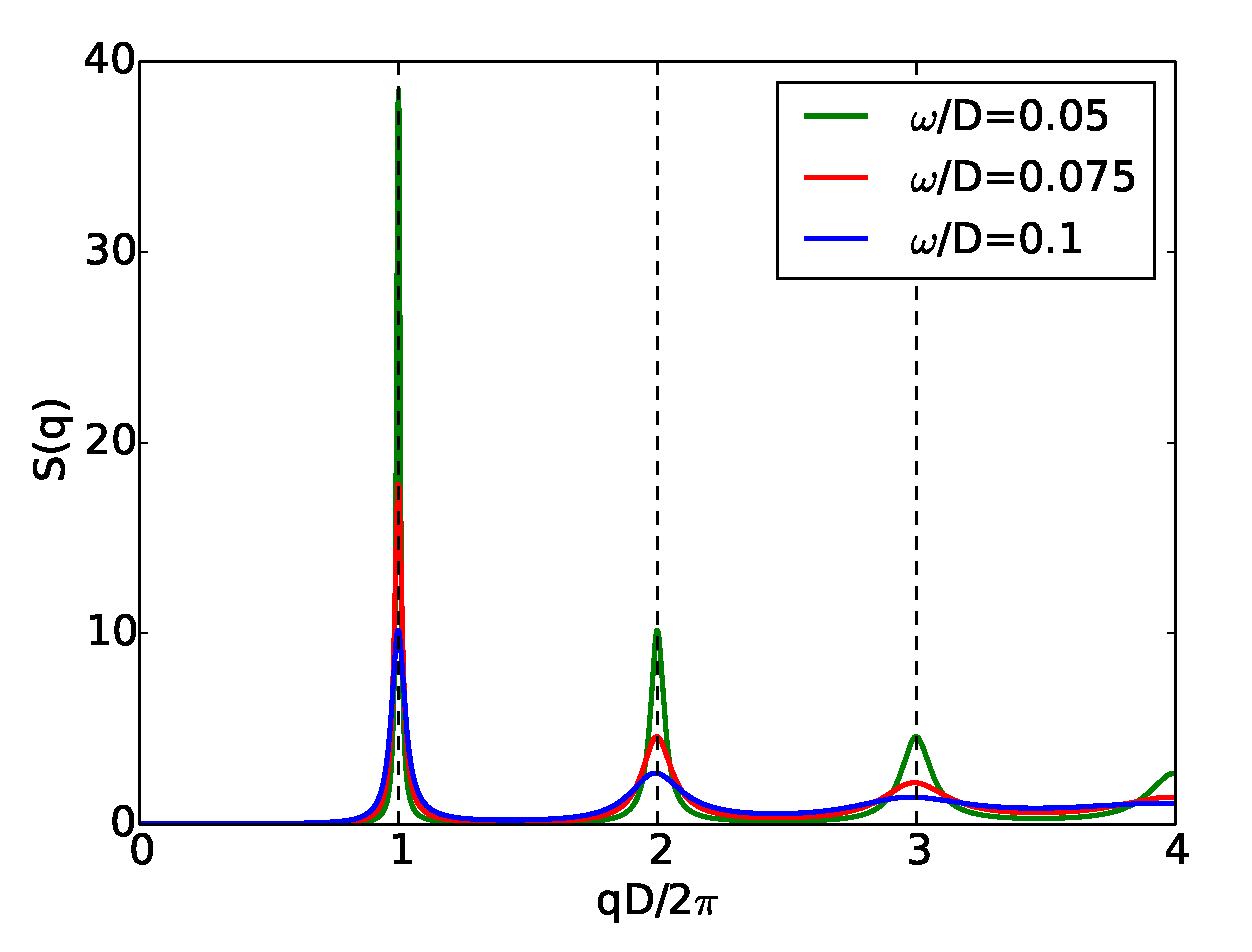
\includegraphics[width=0.6\textwidth]{fig/funcplot/S_q_1Dparacrystal.eps}
\end{center}
\caption{Interference function of a 1D Gaussian paracrystal plotted for different values of $\omega /D$. The peaks broaden with a decreasing amplitude as $\omega/D$ increases. This shows the transition between an ordered and a disordered states. }
\label{fig:1dparas_q}
\end{figure}

In two dimensions, the paracrystal is constructed on a pseudo-regular lattice with base vectors $\v{a}$ and $\v{b}$ using the following conditions for the densities of probabilities:\\
$\int p_{\v{a}}(\r)\d^2r=\int p_{\v{b}}(\r)\d^2r=1$,
$\int \r p_{\v{a}}(\r)\d^2r=\v{a}$,
$\int \r p_{\v{b}}(\r)\d^2r=\v{b}$.

In the ideal case the deformations along the two axes are decoupled
and each unit cell should retain a parallelogram shape.
The interference function is given by
$S(q_{\plll})=\prod_{k=a,b}\Re\left(\dfrac{1+P_k(q_{\plll})}{1-P_k(q_{\plll})} \right)$
with $P_k$ the Fourier transform of $p_k$, $k=a, b$.

\paragraph{Probability distributions} \mbox{}\\
The scattering by an ordered lattice gives rise to a series of Bragg peaks situated at the nodes of the reciprocal lattice. Any divergence from the ideal crystalline case modifies the output spectrum by, for example, widening or attenuating the Bragg peaks. The influence of these "defects" can be accounted for
 in direct space by using correlation functions or by truncating the lattice or, in reciprocal space with structure factors or interference functions by convoluting the scattered peaks with a function which could reproduce the experimental shapes.

%===============================================================================
\subsection{Size-Spacing Correlation Approximation}
%===============================================================================
\index{Size-spacing correlation approximation}

TO MERGE IN:
introduces correlations between polydisperse particles, more precisely between the size of the particles and their mutual spacing. A classical example would consist in particles whose closest-neighbor spacing depends linearly on the sum of their respective sizes \cite{LaLR07}, as illustrated in \cref{fig:ssca}.

%For a sample where only the statistical properties of particle positions and size are known, the scattered intensity per scattering particle is expressed as the average over an ensemble of the Fourier transform of the Patterson function, which is the autocorrelation of the SLD $\curlp (\r ) \equiv \sum_{ij} S_i(-\r )\otimes S_j(\r )\otimes \delta (\r + \r_i - \r_j )$:
%\begin{equation*}
%  I(\q ) = \frac{1}{N}\ensavg{}{\curlf (\curlp (\r ))},
%\end{equation*}
%where $\curlf$ denotes the Fourier transform and $\curlp$ the Patterson function

\begin{figure}[tb]
\begin{center}
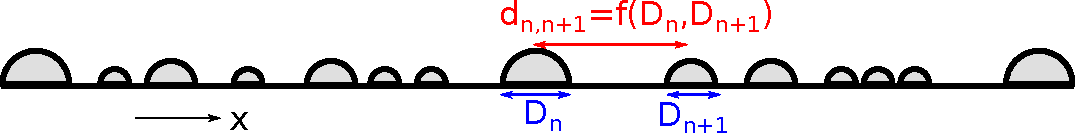
\includegraphics[width=0.9\textwidth]{fig/drawing/drawingSSCA.pdf}
\end{center}
\caption{Sketch of a 1D distributed collection of particles, whose scattering could be described by the size-spacing correlation approximation: the distance between two particles depends on their sizes.}
\label{fig:ssca}
\end{figure}


In the Size-Spacing Correlation Approximation, a correlation is assumed between the shape/size of the particles and their mutual spacing. A classical example would consist of particles whose closest-neighbor spacing depends linearly on the sum of their respective sizes. The following discussion of this type of correlation is inspired by \cite{LaLR07}

The scattered intensity can also be calculated as the Fourier transform of the Patterson function, which is the autocorrelation of the SLD:
\begin{equation*}
  \curlp (\r ) \equiv \sum_{ij} S_i(-\r )\otimes S_j(\r )\otimes \delta (\r + \r_i - \r_j ).
\end{equation*}
For a sample where only the statistical properties of particle positions and shape/size are known, the scattered intensity per scattering particle becomes average over an ensemble of the Fourier transform of the Patterson function:
\begin{equation*}
  I(\q ) = \frac{1}{N}\bra\curlf (\curlp (\r ))\ket,
\end{equation*}
where $\curlf$ denotes the Fourier transform.

The ensemble averaged Patterson function will be denoted as:
\begin{equation*}
  Z(r) \equiv \frac{1}{N}\bra\curlp (\r )\ket.
\end{equation*}
In the case of systems where the particles are aligned in one dimension, this autocorrelation function can be further split into nearest neighbor probabilities. First, it is split into terms for negative, zero or positive distance:
\begin{equation*}
  Z(\r ) \equiv z_0(\r ) + z_+(\r ) + z_-(\r ).
\end{equation*}
Taking $x$ as the coordinate in the direction in which the particles are arranged and $s$ as an orthogonal coordinate ($\r \equiv (x,s)$), one obtains:
\begin{align*}
  z_0(\r ) &= \sum_{\alpha_0} p(\alpha_0) S_{\alpha_0}(-x,-s) \otimes S_{\alpha_0}(x,s)  \\
  z_+(\r ) &= \sum_{\alpha_0\alpha_1} p(\alpha_0,\alpha_1) S_{\alpha_0}(-x,-s) \otimes S_{\alpha_1}(x,s) \otimes P_1(x|\alpha_0\alpha_1)  \\
               &+ \sum_{\alpha_0\alpha_1\alpha_2} p(\alpha_0,\alpha_1,\alpha_2) S_{\alpha_0}(-x,-s) \otimes S_{\alpha_2}(x,s) \otimes P_1(x|\alpha_0\alpha_1) \otimes P_2(x|\alpha_0\alpha_1\alpha_2)  \\
               &+ \dotsb \\
  z_-(\r ) &= z_+(-\r ),
\end{align*}
where $p(\alpha_0,\dotsc ,\alpha_n)$ denotes the probability of having a sequence of particles of the indicated sizes/shapes and $P_n(x|\alpha_0\dotsc\alpha_n)$ is the probability density of having a particle of type $\alpha_n$ at a (positive) distance $x$ of its nearest neighbor of type $\alpha_{n-1}$ in a sequence of the given order.

In the Size-Spacing Correlation Approximation, one assumes that the particle sequence probabilities are just a product of their individual fractions:
\begin{equation*}
  p(\alpha_0,\dotsc ,\alpha_n) = \prod_i p(\alpha_i),
\end{equation*}
and the nearest neighbor distance distribution is dependent only on the two particles involved:
\begin{equation*}
  P_n(x|\alpha_0\dotsc\alpha_n) = P_1(x|\alpha_{n-1}\alpha_n).
\end{equation*}
Furthermore, the distance distribution $P_1(x|\alpha_0\alpha_1)$ depends on the particle sizes/shapes only through its mean value $D$:
\begin{equation*}
  P_1(x|\alpha_0\alpha_1) = P_0(x - D(\alpha_0,\alpha_1) ),
\end{equation*}
where $D(\alpha_0,\alpha_1) = D_0 + \kappa \left[ \Delta R(\alpha_0) + \Delta R(\alpha_1) \right]$, with $\Delta R(\alpha_i)$ the deviation of a size parameter of particle $i$ with respect to the mean over all particles sizes/shapes and $\kappa$ the coupling parameter.

In momentum space, the sum of convolutions can be written as a geometric series, which can be exactly calculated to be:
\begin{equation}
\label{Esscainf}
I(\q ) = {\bra\left| F_\alpha(\q ) \right| ^2\ket}_{\alpha}
+ 2 \Re \left\lbrace \widetilde{\curlf_\kappa}(\q )
 \widetilde{\curlf_\kappa^*}(\q ) \cdot
 \frac{\Omega_\kappa(\q )}{\tilde{p}_{2\kappa}(\q )\left
   [ 1 - \Omega_\kappa(\q )\right] } \right\rbrace,
\end{equation}
with
\begin{align*}
  \tilde{p}_\kappa(\q ) &= \int \d\alpha\; p(\alpha) \e^{i\kappa q_x \Delta R(\alpha)}  \\
  \Omega_\kappa(\q ) &= \tilde{p}_{2\kappa}(\q ) \phi(\q) \e^{i q_x D_0}  \\
  \widetilde{\curlf_\kappa}(\q ) &=
       \int \d\alpha\; p(\alpha)F_\alpha (\q ) \e^{i\kappa q_x \Delta R(\alpha)},
\end{align*}
and the Fourier transform of $P_1(x|\alpha_0\alpha_1)$ is
\begin{equation*}
  \curlp (\q ) = \phi (\q )\e^{i q_x D_0}
                    \e^{i \kappa q_x \left[ \Delta R(\alpha_0) + \Delta R(\alpha_1) \right] }.
\end{equation*}

Using the result from the one-dimensional analysis, one can apply this formula ad hoc for distributions of particles in a plane, where the coordinate $x$ will now be replaced with $(x,y)$, while the $s$ coordinate encodes a position in the remaining orthogonal direction. One must be aware however that this constitutes a further approximation, since this type of correlation does not have a general solution in more than one dimension.

The intensity in \cref{Esscainf} will contain a Dirac delta function contribution, caused by taking an infinite sum of terms that are perfectly correlated at $\q = 0$. One can leverage this behaviour by multiplying the nearest neighbor distribution by a constant factor $\e^{-D/\Lambda}$, which removes the division by zero in \cref{Esscainf}.
Another way of dealing with this infinity at $\q =0$ consists of taking only a finite number of terms, in which case the geometric series still has an analytic solution, but becomes a bit more cumbersome:
\begin{equation*}
\begin{split}
  I(\q ) &= {\bra\left| F_\alpha(\q ) \right| ^2\ket}_\alpha
   + 2 \Re \Biggl\lbrace \frac{1}{\tilde{p}_{2\kappa}(\q )}\widetilde{\curlf_\kappa}(\q )\widetilde{\curlf_\kappa^*}(\q ) \\
  & \times \left[ \left( 1 - \frac{1}{N}\right) \frac{\Omega_\kappa(\q )}{1 - \Omega_\kappa(\q ) } - \frac{1}{N}\frac{\Omega_\kappa^2(\q )\left( 1- \Omega_\kappa^{N-1}(\q )\right) }{\left( 1 - \Omega_\kappa(\q ) \right) ^2 } \right] \Biggr\rbrace.
\end{split}
\end{equation*}
This expression has a well-defined limit for $\Omega_\kappa(\q ) \rightarrow 1$ (when $\q \rightarrow 0$), namely:
\begin{equation*}
  \lim_{\q \rightarrow 0} I(\q ) = {\bra\left| F_\alpha(0 ) \right| ^2\ket}_{\alpha} + \left( N-1 \right) \left| {\bra F_\alpha(0 )\ket}_{\alpha} \right|^2.
\end{equation*}


%%%%%%%%%%%%%%%%%%%%%%%%%%%%%%%%%%%%%%%%%%%%%%%%%%%%%%%%%%%%%%%%%%%%%%%%%%%%%%%%
\section{Vertical location of particles}
%%%%%%%%%%%%%%%%%%%%%%%%%%%%%%%%%%%%%%%%%%%%%%%%%%%%%%%%%%%%%%%%%%%%%%%%%%%%%%%%

 \Note{The particles cannot sit in between layers. At most they can be sitting on any inner interfaces.}

%===============================================================================
\subsection{Particles deposited on a substrate}
%===============================================================================
%Substrate modified Born approximation
In this configuration, the particles are sitting on top of a substrate layer in air or vacuum.
In the DWBA the expression of a form factor becomes
\begin{align}
F_{\rm{DWBA}}(q_{\plll}, k_{i,z}, k_{f,z}) &= F_{\rm{BA}}(q_{\plll}, k_{i,z}-k_{f,z})+ R_i F_{\rm{BA}}(q_{\plll}, -k_{i,z}-k_{f,z}) \nonumber \\
&+ R_f F_{\rm{BA}}(q_{\plll}, k_{i,z}+k_{f,z}) + R_i R_f F_{\rm{BA}}(q_{\plll},-k_{i,z}+k_{f,z}), \label{Edwbaair}
\end{align}
where $q_{\plll}$ is the component of the scattering beam in the plane of the interface ($\q=\k_i-\k_\sf$), $k_{i,z}$ and $k_{f,z}$ are the z-component of the incident and scattered beam, respectively. $R_i$, $R_f$ are the reflection coefficients in incidence and reflection. They are defined as\\ $R=\dfrac{k_z+\sqrt{n_s^2k_0^2-|k_{\plll}|^2}}{k_z-\sqrt{n_s^2 k_0^2-|k_{\plll}|^2}}$, where $n_s=1-\delta_s +i \beta_s$ is the refractive index of the substrate, $k_0$ is the wavelength in vacuum ($2\pi /\lambda$), $k_z$ and $k_{\plll}$ are the $z$-component and the in-plane component of $\k_\si$ or $\k_\sf$. \\

\Note{If the particles are sitting on a multilayered system, the expression of the form factor in the DWBA is obtained by replacing the Fresnel coefficient by the corresponding coefficients of the underlying layers \cite{Par54,BoWo99}.}

Script~\ref{lst:badwba} illustrates the difference between BA and DWBA in \BornAgain\ when generating the sample.  We consider the simple case of:
\begin{itemize}
\item one kind of particles' shape,
\item no interference between the particles,
\item in the DWBA, a sample made of a layer of substrate on which are deposited the particles,
\item in the BA, a sample composed of the particles in air.
\end{itemize}

\Cref{fig:spheroidbadwba} shows the intensity contour plot generated using this script with truncated spheroids as particles.

\newpage

\begin{lstlisting}[language=python, style=eclipseboxed,numbers=none,nolol,caption={\Code{Python} script to generate a sample using Born (BA) or distorted-wave Born approximation (DWBA). The difference between BA and DWBA in this simple case is the absence or presence of a substrate layer in the sample.},label={lst:badwba}]
def get_sample():
    """
    Build and return the sample to calculate form factor of
    truncated spheroid in Born or distorted-wave Born Approximation.
    """
    # defining materials
    m_ambience = HomogeneousMaterial("Air", 0.0, 0.0)
    m_substrate = HomogeneousMaterial("Substrate", 6e-6, 2e-8)
    m_particle = HomogeneousMaterial("Particle", 6e-4, 2e-8)

    # collection of particles
    ff= FormFactorTruncatedSpheroid(7.5*nanometer, 9.0*nanometer, 1.2)
    particleshape = Particle(m_particle, ff)
    particle_layout = ParticleLayout()
    particle_layout.addParticle(particleshape, 1.0)

    # interferences
    interference = InterferenceFunctionNone()
    particle_layout.addInterferenceFunction(interference)

    # assembling the sample
    air_layer = Layer(m_ambience)
    air_layer.addLayout(particle_layout)
    substrate_layer = Layer(m_substrate, 0)

    multi_layer = MultiLayer()
    multi_layer.addLayer(air_layer)
    # Comment the following line out for Born Approximation
    multi_layer.addLayer(substrate_layer)
    return multi_layer
\end{lstlisting}


\begin{figure}[tb]
\hfill
\subfigure[Born Approximation]{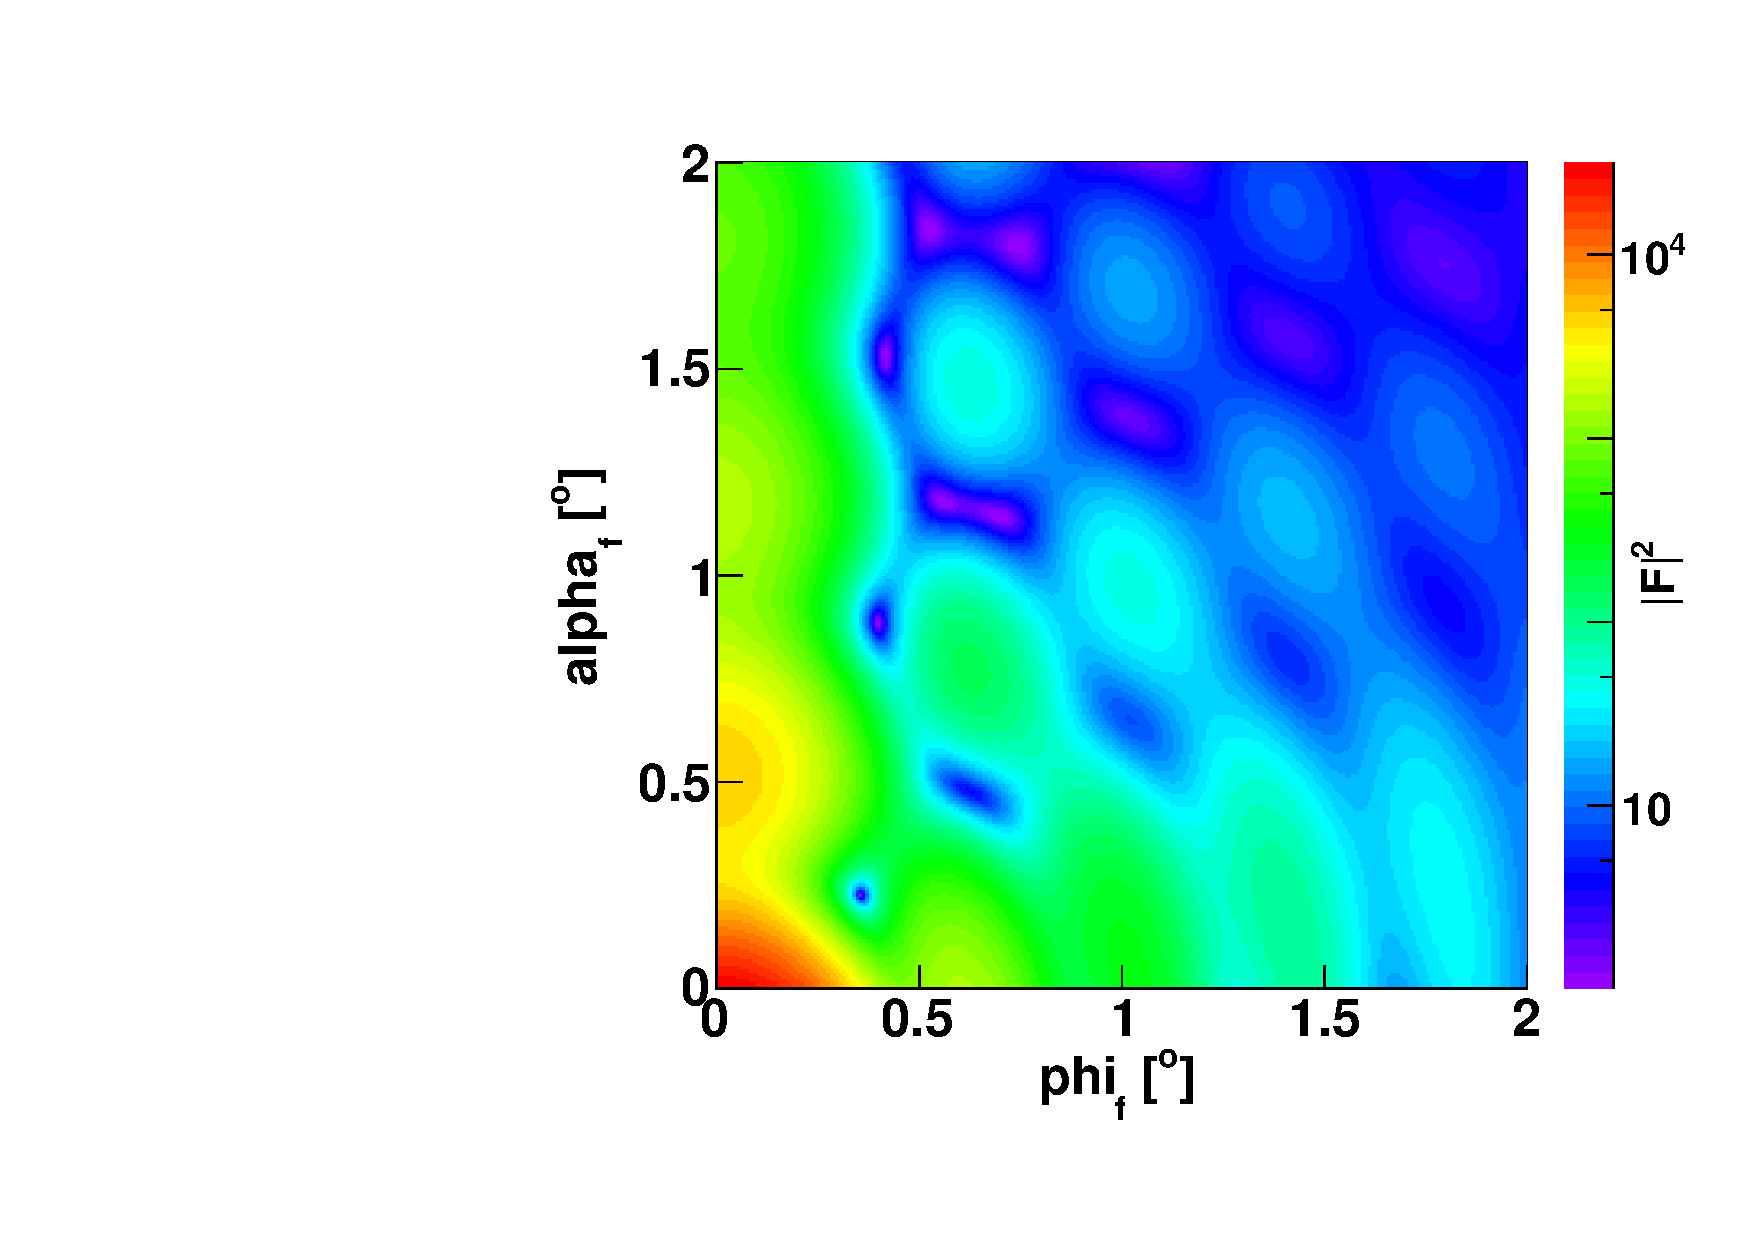
\includegraphics[angle=-90,width=6cm]{fig/gisasmap/ffspheroidBA.pdf}}
\hfill
\subfigure[DWB Approximation]{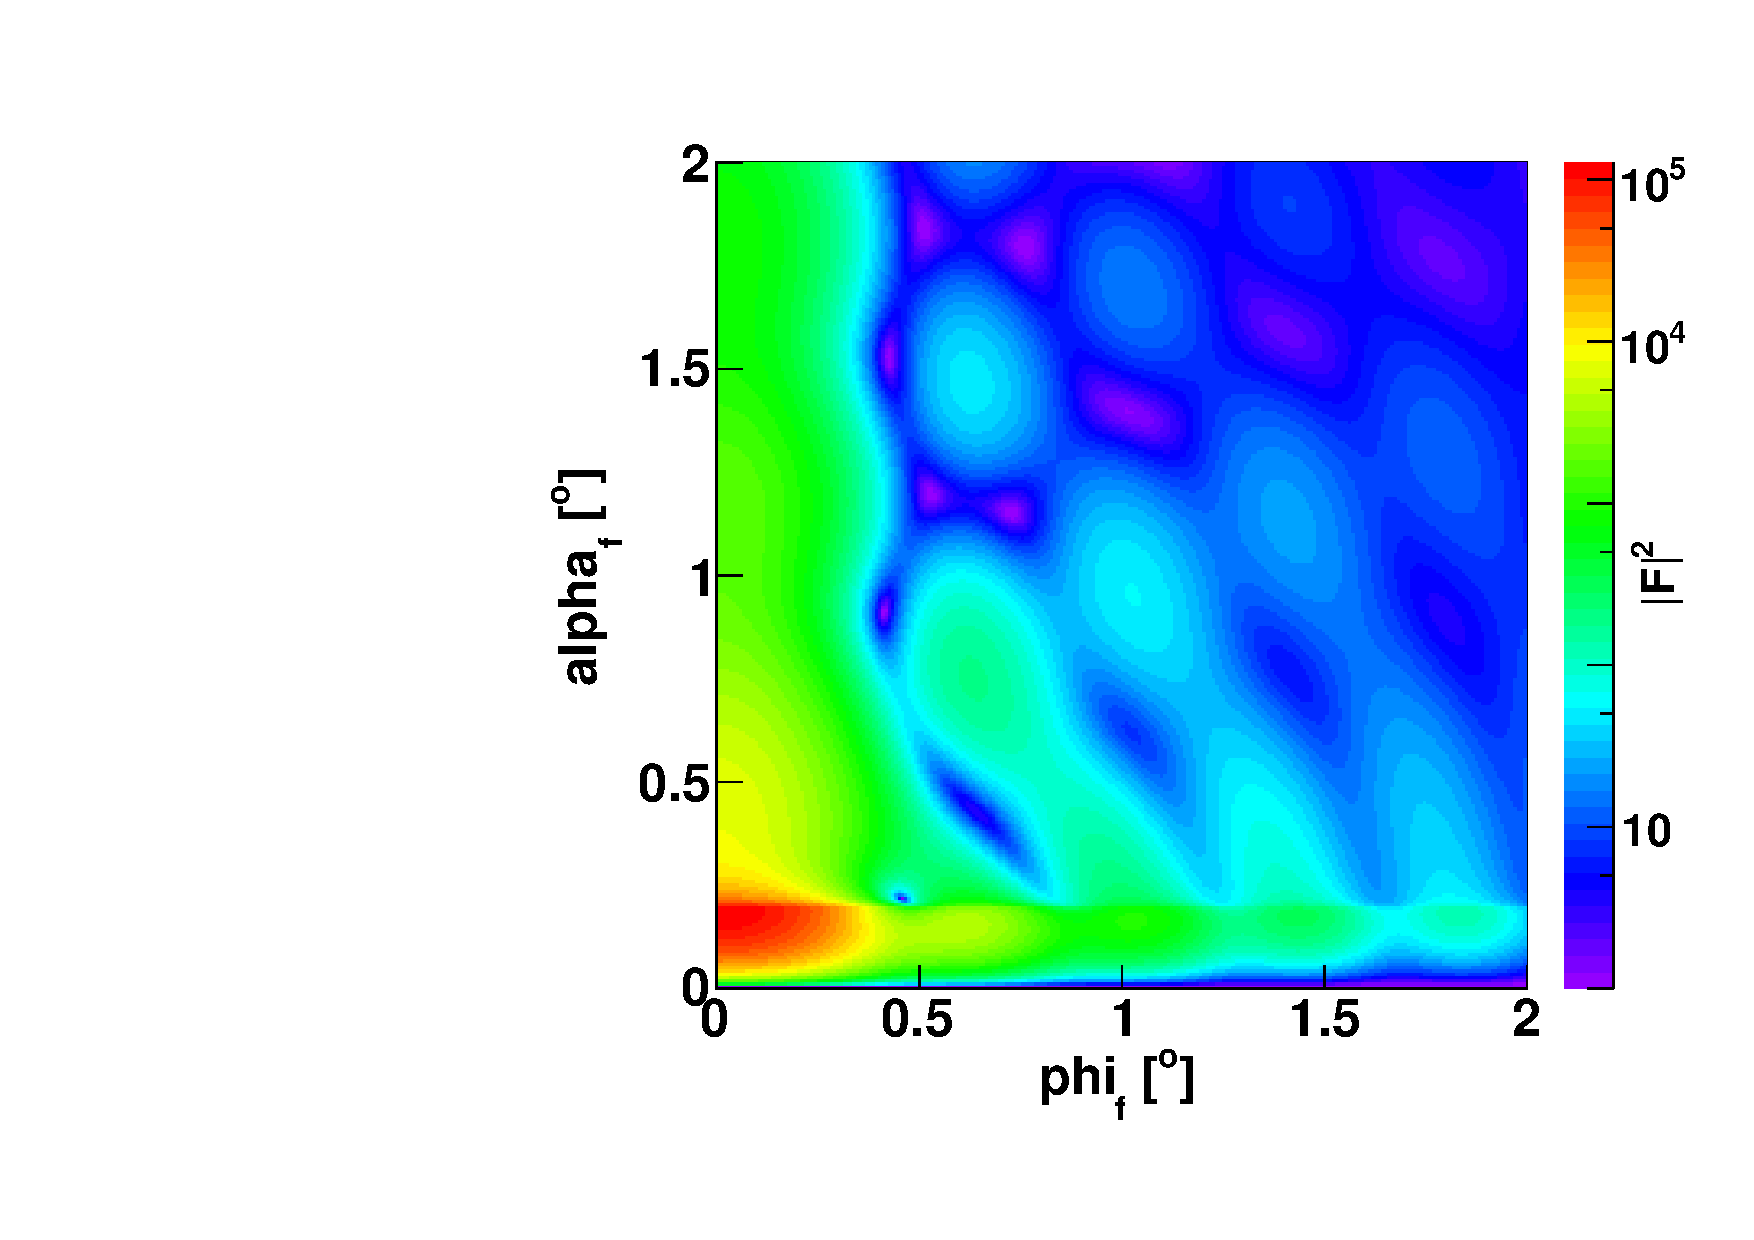
\includegraphics[angle=-90,width=6cm]{fig/gisasmap/ffspheroidDWBA.pdf}}
\hfill
\caption{Intensity map of TruncatedSpheroid form factor in BA and DWBA computing using script~\ref{lst:badwba} for the sample.}
\label{fig:spheroidbadwba}
\end{figure}

\FloatBarrier

\Note{In \BornAgain, the DWBA is implemented automatically when assembling the sample with more layers than only the air layer (for example, for particles are sitting on a substrate).}

%===============================================================================
\subsection{Buried particles}
%===============================================================================

The system considered in this section consists of particles encapsulated in a layer, which is sitting on a substrate. In this case the form factor in the DWBA is given by

\begin{align}
  F_{\rm{DWBA}}(q_{\plll}, k_{i,z}, k_{f,z})
  &= T_\si T_\sf F_{\rm{BA}}(q_{\plll}, k_{i,z}-k_{f,z})\e^{i(k_{i,z}-k_{f,z})d}\nonumber \\
  &+ R_\si T_\sf F_{\rm{BA}}(q_{\plll}, -k_{i,z}-k_{f,z})\e^{i(-k_{i,z}-k_{f,z})d} \nonumber \\
  &+ R_\sf T_\si F_{\rm{BA}}(q_{\plll}, k_{i,z}+k_{f,z}) \e^{i(k_{i,z}+k_{f,z})d}\nonumber \\
  &+ R_\sf R_\si F_{\rm{BA}}(q_{\plll},-k_{i,z}+k_{f,z})\e^{i(-k_{i,z}+k_{f,z})d}, \label{Edwbaburied}
\end{align}

\begin{equation*}
R_j =\frac{t^{j}_{0,1}r^{j}_{1,2}\exp(2ik_{j,z}t)}{1+r^{j}_{0,1}r^{j}_{1,2}\exp(2ik_{j,z}t)}, \quad T_j=\frac{t^{j}_{0,1}}{1+r^{j}_{0,1}r^{j}_{1,2}\exp(2ik_{j,z}t)}, j=i,f
\end{equation*}
where $q_{\plll}$ is the component of the scattering beam in the plane of the interface, $k_{i,z}$ and $k_{f,z}$ are the z-component of the incident and scattered beams, respectively.  $d$ is the depth at which the particles are sitting in the layer. Note that this value is given relative to the top of this layer and it is not the coordinate in the absolute referential (linked with the full sample) and it is measured up to the bottom of the particle. $t$ is the thickness of the intermediate layer containing the particles. $R_{i,f}$ and $T_{i,f}$  are the reflection  and transmission coefficients in incidence and reflection (they can be calculated using Parratt or matrix formalism). $r^j_{0,1}$, $r^j_{1,2}$ $t^j_{0,1}$ are the reflection and transmission coefficients between layers; the indices are related to different boundaries with 0: air, 1: intermediate layer and 2: substrate layer and the superscript $j$ is associated with the incident or scattered beams:
\begin{equation*}
r^j_{n,n+1}=\frac{k_{j,z,n}-k_{j,z,n+1}}{k_{j,z,n}-k_{j,z,n+1}}, \qquad t^j_{n,n+1}= \frac{2k_{j,z,n}}{k_{j,z,n}-k_{j,z,n+1}}, \quad n=0,1, \quad j=i,f,
\end{equation*}
where index $n$ is related to the layers, $z$ to the vertical component, and $j$ to the beams (incident and outgoing).

\Cref{fig:dwbaburied} shows a typical example of the output intensity scattered from a sample made of 3 layers: air, substrate, and in between, spherical particles embedded in the middle of a 30~nm-thick layer. This figure had been generated using listing~\ref{lst:dwbaburied}.

\begin{lstlisting}[language=python, style=eclipseboxed,numbers=none,nolol,caption={\Code{Python} script to generate a sample where spherical particles are embedded in the middle of a layer on a substrate.},label={lst:dwbaburied}]
def get_sample():
    """
    Build and return the sample with buried spheres in DWBA.
    """
    # defining materials
    m_ambience = HomogeneousMaterial("Air", 0.0, 0.0)
    m_interm_layer = HomogeneousMaterial("IntermLayer",3.45e-6, 5.24e-9)
    m_substrate = HomogeneousMaterial("Substrate", 7.43e-6, 1.72e-7)
    m_particle = HomogeneousMaterial("Particle", 0.0, 0.0)

    # collection of particles
    ff = FormFactorFullSphere(10.2*nanometer)
    particleshape = Particle(m_particle, ff)
    particleshape.setPosition(0.0, 0.0, -25.2)
    particle_layout = ParticleLayout()
    particle_layout.addParticle(particleshape, 1.0)

    # interferences
    interference = InterferenceFunctionNone()
    particle_layout.addInterferenceFunction(interference)

    # assembling the sample
    air_layer = Layer(m_ambience)
    intermediate_layer = Layer(m_interm_layer, 30.*nanometer)
    intermediate_layer.addLayout(particle_layout)
    substrate_layer = Layer(m_substrate, 0)

    multi_layer = MultiLayer()
    multi_layer.addLayer(air_layer)
    multi_layer.addLayer(intermediate_layer)
    multi_layer.addLayer(substrate_layer)
    return multi_layer
\end{lstlisting}


\begin{figure}[tb]
\centering
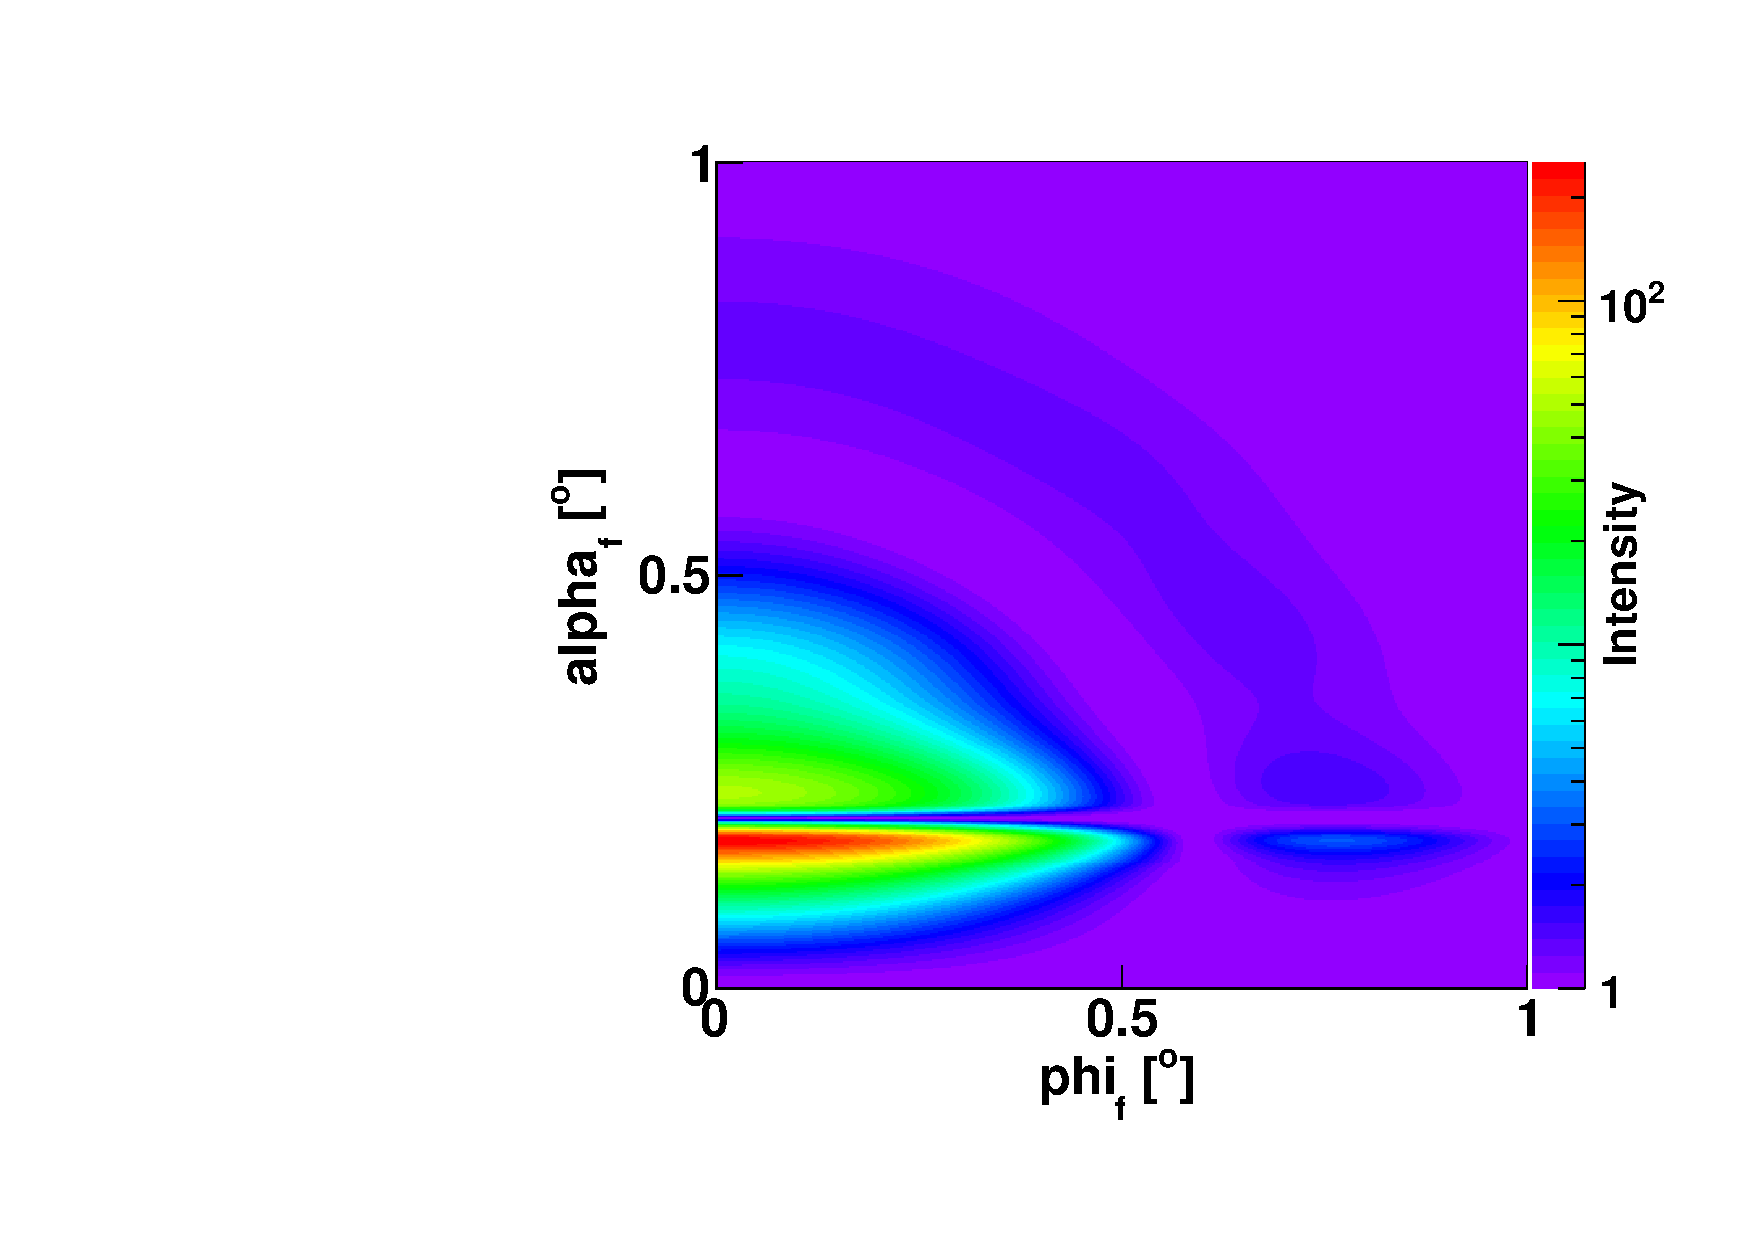
\includegraphics[angle=-90,width=0.6\textwidth]{fig/gisasmap/figIntBuriedPart.pdf}
\caption{Map of intensity scattered from a sample made of spherical particles embedded in the middle of a 30~nm-thick layer on a substrate (see Script~\ref{lst:dwbaburied} for details about the sample).}
\label{fig:dwbaburied}
\end{figure}

\newpage

\Note{For layers different from the air layer, the top interface is considered as the reference level to position the encapsulated particles. For example, spheres positioned at depth $d$ (positive) are located at a distance $d$ from the top of the layer up to the bottom of these particles. This convention is different for the top air layer, where particles sitting at the interface with an underlying layer (\idest the bottom of the air layer) are located at depth 0 (see \cref{fig:depthpartBA}).}


\begin{figure}[tb]
\centering
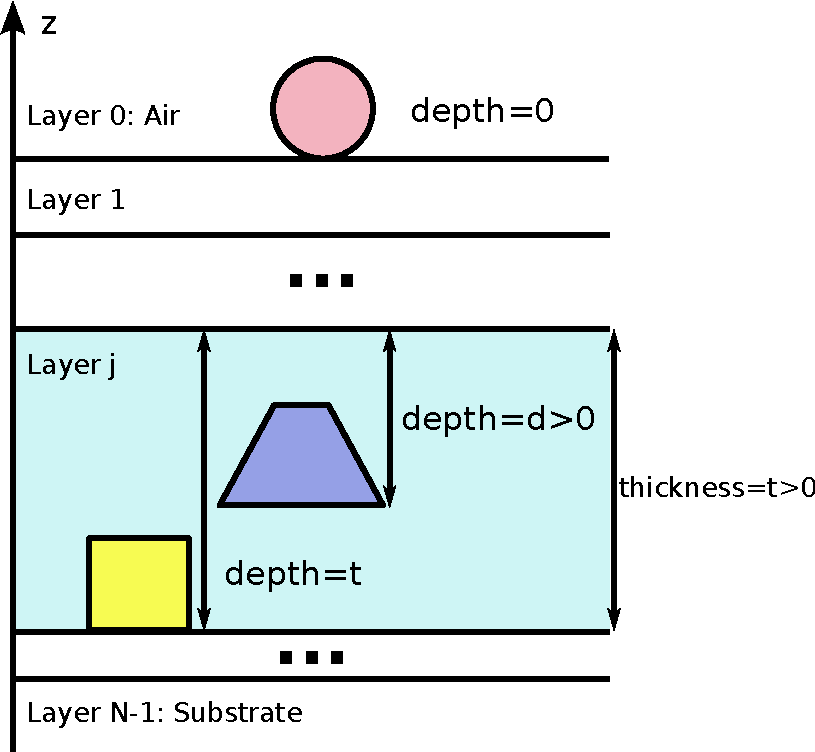
\includegraphics[width=0.5\textwidth]{fig/drawing/drawingDepthParticle.pdf}
\caption{Illustration of the convention about \Code{depth} used in \BornAgain\ to encapsulate particles in layers.}
\label{fig:depthpartBA}
\end{figure}


%%%%%%%%%%%%%%%%%%%%%%%%%%%%%%%%%%%%%%%%%%%%%%%%%%%%%%%%%%%%%%%%%%%%%%%%%%%%%%%%
\section{Implementation in \BornAgain}
%%%%%%%%%%%%%%%%%%%%%%%%%%%%%%%%%%%%%%%%%%%%%%%%%%%%%%%%%%%%%%%%%%%%%%%%%%%%%%%%

This section describes the implementation of the interference functions in \BornAgain.
For an implementation of all the components of a simulation,
the use is referred, for example, to \cref{sec:Example1Python}.\\


\Note{In \BornAgain\ the particles are positioned in the same vertical layer.}

\subsection{Size-distribution models}
\index{Size-distribution models}
The decoupling approximation (DA), local monodisperse approximation (LMA) and size spacing correlation approximation (SSCA) can be used in \BornAgain.
The selection between DA and SSCA is made using\\
\Code{ILayout.setApproximation(EInterferenceFunction approximation)} when defining the characteristics of the way particles and interference functions are embedded in a layer.  For example,
\begin{lstlisting}[language=python, style=eclipseboxed,numbers=none,nolol]
    particle_layout = ParticleLayout()
   ....
# interference approx chosen between: DA (default) and SSCA
    particle_layout.setApproximation(ILayout.DA)
\end{lstlisting}

Note that with the SSCA, the users have to specify the coupling parameter $\kappa$ (with the function \Code{setKappa}), which should be a positive dimensionless value. $\kappa$ characterizes the influence of the neighboring particles' sizes on their distance. If $\kappa=0$, the SSCA reduces to the DA with a radial paracrystal for the interference function.\\

For the LMA, its implementation is automatically done when using more than one layout of particles:
\begin{lstlisting}[language=python, style=eclipseboxed,numbers=none,nolol]
    particle_layout0 = ParticleLayout()
    particle_layout1 = ParticleLayout()
   ....
# association of each particles' layout with materials, form factors
#... and with a material layer
    layer_a = Layer(m_material_a)
    layer_a.addLayout(particle_layout0)
    layer_a.addLayout(particle_layout1)
\end{lstlisting}

%%ADD EXPLANATION ABOUT LMA

%-------------------------------------------------------------------------------
\subsection{Probability distribution functions}\label{baftd}
%-------------------------------------------------------------------------------

The probability distribution functions have been implemented in the reciprocal space in \BornAgain. Their expressions are given in Table~\ref{table:pdf}.

\begin{table}[H]
\centering
\begin{tabular}{ccc}
\hline
Function & One dimension & Two dimensions\\
\hline
Cauchy & $(1+q^2\omega^2)^{-3/2}$ & $(1 + q_x^2 cl_x^2 + q_y^2 cl_y^2)^{-3/2}$ \\
Gauss & $\dfrac{1}{2}\exp(-\dfrac{q^2\omega^2}{4})$ & $\frac{1}{2}\exp\left(-\dfrac{q_x^2 cl_x^2+ q_y^2cl_y^2}{4}\right)$ \\
Voigt & $\dfrac{\eta}{2} \exp\left(-\dfrac{q^2\omega^2}{4}\right) + \dfrac{1 - \eta}{(1 + q^2\omega^2)^{3/2}}$ & $\dfrac{\eta}{2} \exp\left(-\dfrac{q_x^2 cl_x^2+ q_y^2cl_y^2}{4}\right)+ \dfrac{1 - \eta}{(1 + q_x^2 cl_x^2+ q_y^2cl_y^2)^{3/2}}$ \\
\hline
\end{tabular}
\caption{List of probability distribution functions in reciprocal space. $\omega$, $cl$ stand for coherence lengths (the index refers to the axis) and  $\eta$ is a weighting coefficient.}
\label{table:pdf}
\end{table}

The Cauchy distribution corresponds to $\exp(-r)$ in real space and the Voigt one  is a linear combination of the Gaussian and Cauchy probability distribution functions.\\

\noindent \underline{One dimension}
\begin{itemize}
\item \Code{FTDistribution1DCauchy($\omega$)},
\item \Code{FTDistribution1DGauss($\omega$)},
\item \Code{FTDistribution1DVoigt($\omega, \eta$)}.
\end{itemize}
where $\omega$ is the coherence length and $\eta$ is a weighting factor.\\

\noindent \underline{Two dimensions}
\begin{itemize}
\item \Code{FTDistribution2DCauchy($cl_x$, $cl_y$)},
\item \Code{FTDistribution2DGauss($cl_x$, $cl_y$)},
\item \Code{FTDistribution2DVoigt($cl_x$, $cl_y$)}
\end{itemize}
where $cl_{x,y}$ are the coherence lengths in the $x$ or $y$ direction, respectively.

These functions can be used with all interference functions, except the case without any interference.

%-------------------------------------------------------------------------------
\subsection{Interferences}
%-------------------------------------------------------------------------------
\index{Interference function}

The interference function is specified when building the sample. It is linked with the particles (shape, material). Examples of implementation are given at the end of each description.

\paragraph{Syntax:}
 \Code{particle\_layout.addInterferenceFunction(interference\_function)},\\ where \Code{particle\_layout} holds the information about the different shapes and their proportions for a given layer of particles, and \Code{interference\_function}  is one of the following expressions:
\begin{itemize}
\item \Code{InterferenceFunctionNone()}
\item \Code{InterferenceFunction1DLattice(lattice\_parameters)}
\item \Code{InterferenceFunctionRadialParaCrystal(peak\_distance, damping\_length)}
\item \Code{InterferenceFunction2DLattice(lattice\_parameters)}
\item \Code{InterferenceFunction2DParaCrystal(length\_1, length\_2, $\alpha$\_lattice, $\xi$, \\ damping\_length)}
\end{itemize}

\Note{\Code{InterferenceFunction1DLattice} can only be used for particles which are infinitely long in one direction of the sample's surface like for example a rectangular grating.}

\newpage
%-------------------------------------------------------------------------------
\subsection{InterferenceFunctionNone}
%-------------------------------------------------------------------------------

The particles are placed randomly in the dilute limit and are considered as individual, non-interacting scatterers. The scattered intensity is function of the form factors only.

\paragraph{Example} The sample is made of a substrate on which are deposited half-spheres. Script~\ref{lst:nointerf} details the commands necessary to generate such a sample. \Cref{fig:nointerf} shows an example of output intensity: Script~\ref{lst:nointerf}  + detector's + input beam's characterizations.


\begin{figure}[tb]
\begin{center}
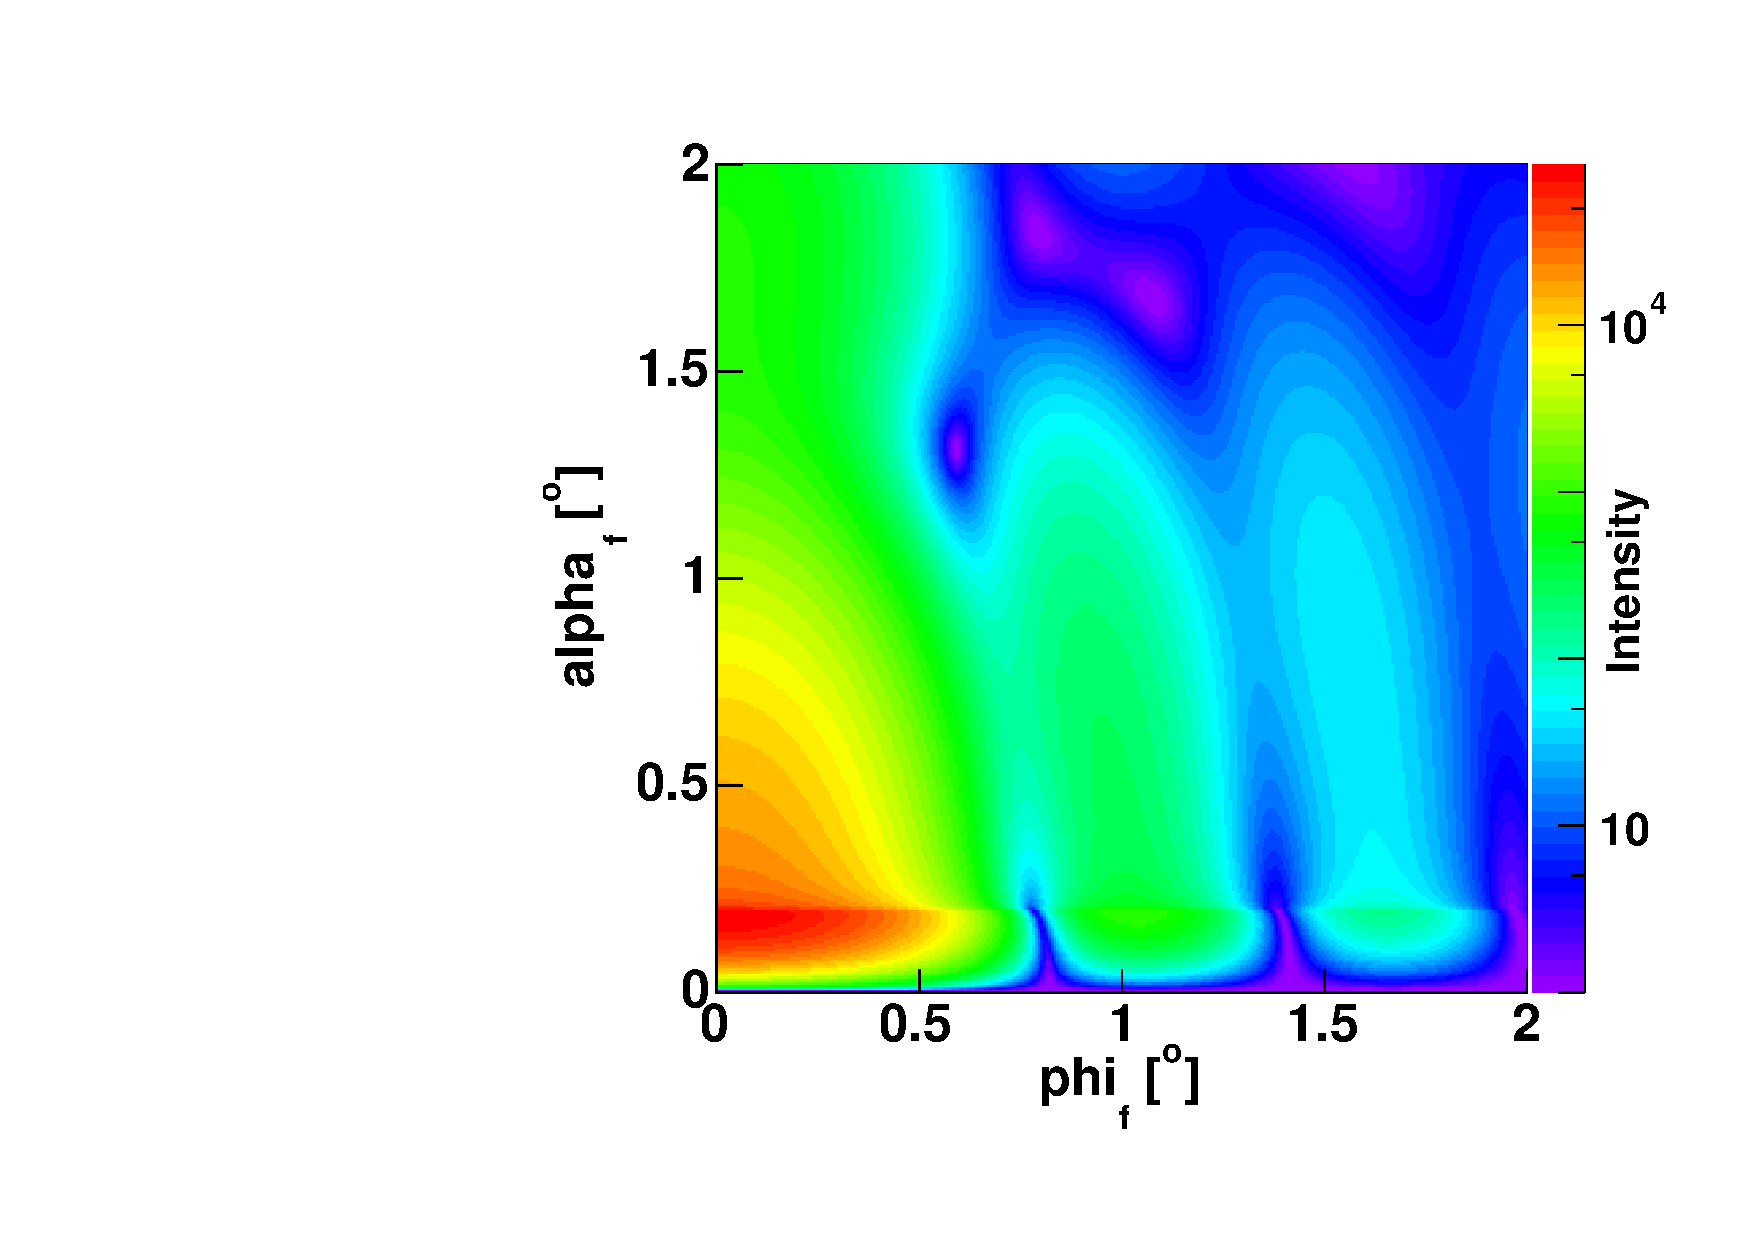
\includegraphics[angle=-90,width=0.5\textwidth]{fig/gisasmap/HSphere_NoInterf.pdf}
\end{center}
\caption{Output intensity scattered from a sample made of half-spheres with no interference between them.}
\label{fig:nointerf}
\end{figure}

\FloatBarrier
\newpage

\begin{lstlisting}[language=python, style=eclipseboxed,numbers=none,nolol,caption={\Code{Python} script to simulate a sample made of half-spheres deposited on a substrate layer without any interference. The part specific to the interferences is marked in a red italic font.},label={lst:nointerf}]
def get_sample():
    """
    Build and return the sample representing particles with no interference
    """
    # defining materials
    m_ambience = HomogeneousMaterial("Air", 0.0, 0.0)
    m_substrate = HomogeneousMaterial("Substrate", 6e-6, 2e-8)
    m_particle = HomogeneousMaterial("Particle", 6e-4, 2e-8)
    # collection of particles
    sphere_ff = FormFactorTruncatedSphere(5*nanometer, 5*nanometer)
    sphere = Particle(m_particle, sphere_ff)
    particle_layout = ParticleLayout()
    particle_layout.addParticle(sphere, 1.0)
    |interference = InterferenceFunctionNone()|
    |particle_layout.addInterferenceFunction(interference)|
    # assembling the sample
    air_layer = Layer(m_ambience)
    air_layer.addLayout(particle_layout)
    substrate_layer = Layer(m_substrate, 0)

    multi_layer = MultiLayer()
    multi_layer.addLayer(air_layer)
    multi_layer.addLayer(substrate_layer)
    return multi_layer
\end{lstlisting}

\newpage
%-------------------------------------------------------------------------------
\subsection{\Code{InterferenceFunction1DLattice(lattice\_length, xi)}}
%-------------------------------------------------------------------------------
where lattice\_length is the lattice constant and $\xi$ the angle in radian between the lattice unit vector and the $\v{x}$-axis of the reference Cartesian frame as shown in \cref{fig:1dgrating}.

\begin{figure}[tb]
\begin{center}
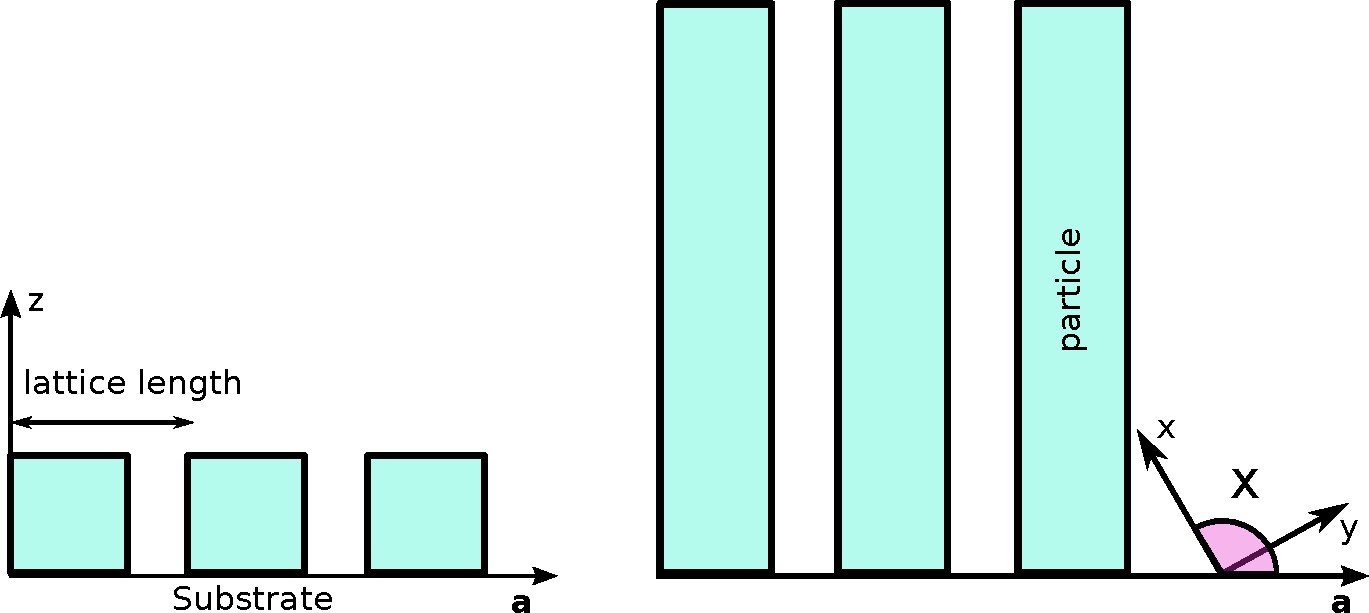
\includegraphics[width=0.75\textwidth]{fig/drawing/1DGrating.pdf}
\end{center}
\caption{Schematic representation of a 1D lattice (side and top views). Such a lattice is characterized by a lattice length and the angle $\xi$.}
\label{fig:1dgrating}
\end{figure}

\Note{By default the long axis of the particles in this 1D lattice is along the beam axis. That is the reason why in the example below the particles are rotated by  $90^{\circ}$ in the $(x,y)$ plane: the main axis of the lattice is therefore parallel to the y-axis, perpendicular to the long axis of the particles.}

\vspace{12pt}
A probability distribution function \Code{pdf} has to be chosen from the list in \cref{baftd} in order to apply some modifications to the scattering peaks. This function is implemented using \Code{setProbabilityDistribution(pdf)}.

\paragraph{Example:} Script~\ref{lst:1dlattinterf} details how to build in  \BornAgain\ a sample using\\ \Code{InterferenceFunction1DLattice} as the interference function. As mentioned previously, this interference function can only be used with infinitely wide or long particles.\\ Here the sample is made of infinitely long boxes deposited on a substrate (these particles are characterized by their widths and heights). They are also rotated by $90^{\circ}$  in the sample surface in order to have their long axis perpendicular to the input beam, which is along the $x$-axis.\\
 The lattice parameters (the lattice length and angle between the lattice main axis and the $x$-axis) are passed into the constructor of the interference function.

\newpage
\begin{lstlisting}[language=python, style=eclipseboxed,numbers=none,nolol,caption={\Code{Python} script to generate a sample made of infinitely long boxes deposited on a substrate layer with the 1DLatticeInterference function. The part specific to the interferences is marked in a red italic font.},label={lst:1dlattinterf}]
def get_sample():
    """
    Build and return the sample with 1DLatticeInterference function
    """
    # defining materials
    m_air = HomogeneousMaterial("Air", 0.0, 0.0)
    m_substrate = HomogeneousMaterial("Substrate", 6e-6, 2e-8)
    m_particle = HomogeneousMaterial("Particle", 6e-4, 2e-8)

    # collection of particles
    ff = FormFactorInfLongBox(10.*nanometer, 15.0*nanometer)
    box = Particle(m_particle, ff)
    particle_layout = ParticleLayout()
    transform = Transform3D.createRotateZ(90.0*degree)
    particle_layout.addParticle(box, transform)

    # interference function
    |interference = InterferenceFunction1DLattice(30.0*nanometer, 0.0*degree)|
    |pdf = FTDistribution1DCauchy(200./2./M_PI*nanometer)|
    |interference.setProbabilityDistribution(pdf)|
    |particle_layout.addInterferenceFunction(interference)|

    # air layer with particles and substrate form multi layer
    air_layer = Layer(m_air)
    air_layer.addLayout(particle_layout)
    substrate_layer = Layer(m_substrate, 0)

    multi_layer = MultiLayer()
    multi_layer.addLayer(air_layer)
    multi_layer.addLayer(substrate_layer)
    return multi_layer
\end{lstlisting}

\newpage
%-------------------------------------------------------------------------------
\subsection{\Code{InterferenceFunctionRadialParaCrystal(peak\_distance, damping\_length)}}
%-------------------------------------------------------------------------------
\begin{itemize}
\item[where] \Code{peak\_distance} is the average distance to the first neighbor peak,
\item[]\Code{width} is the width parameter of the probability distribution,
\item[] \Code{damping\_length} is used to introduce finite size effects by applying a multiplicative coefficient equal to  $\exp$(-\Code{peak\_distance/damping\_length}) to the Fourier transform of the probability densities. \Code{damping\_length} is equal to 0 by default and, in this case, no correction is applied.
\end{itemize}

A probability distribution function \Code{pdf} has to be chosen from the list in \cref{baftd} in order to apply some modifications to the scattering peaks. This function is implemented using \Code{setProbabilityDistribution(pdf)}.


\Note{
This interference function is not one-dimensional.  It takes into account the radial component of the scattering vector.
}

\paragraph{Example}
To illustrate the radial paracrystal interference function, we use the same sample as in the case without interference: half-spheres deposited on a substrate.

\begin{lstlisting}[language=python, style=eclipseboxed,numbers=none,nolol,caption={\Code{Python} script to define the radial paracrystal interference function between half-spheres, where \Code{trsphere} is of type \Code{Particle}.},label={lst:1dpara}]
    particle_layout = ParticleLayout()
    particle_layout.addParticle(trsphere, 1.0)
    interference = InterferenceFunctionRadialParaCrystal(25.0*nanometer, 1e3*nanometer)
    pdf = FTDistribution1DGauss(7 * nanometer)
    interference.setProbabilityDistribution(pdf)
    particle_layout.addInterferenceFunction(interference)
\end{lstlisting}



\begin{figure}[tb]
\begin{center}
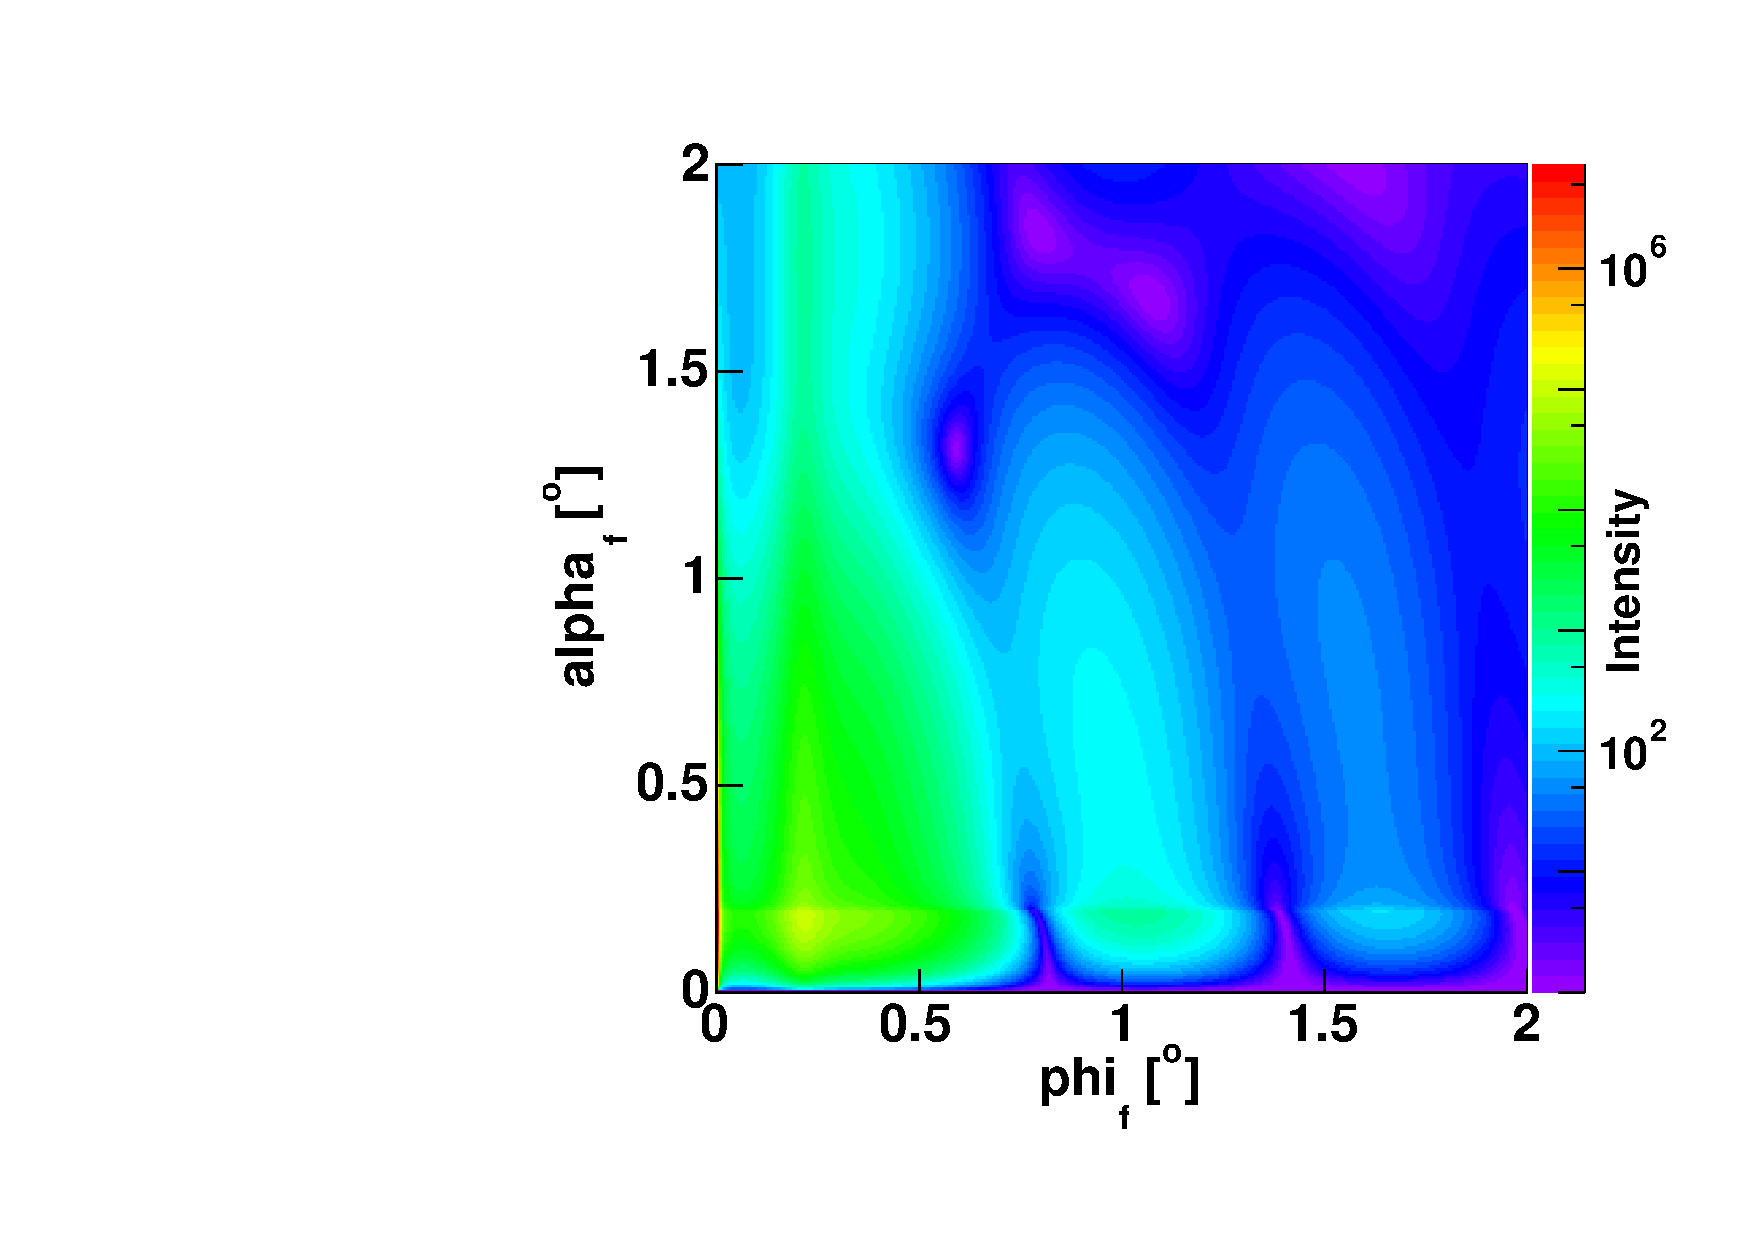
\includegraphics[angle=-90,width=0.5\textwidth]{fig/gisasmap/HSphere_1DDL.pdf}
\end{center}
\caption{Output intensity scattered from a sample made of half-spheres with the radial paracrystal interference between them. This figure has been generated using Script~\ref{lst:1dpara} for the interference function.}
\label{fig:1ddl}
\end{figure}

\FloatBarrier

\newpage
%-------------------------------------------------------------------------------
\subsection{\Code{InterferenceFunction2DLattice(L\_1, L\_2, alpha, xi)}}
%-------------------------------------------------------------------------------
where ($L_1$, $L_2$, $\alpha$, $\xi$) are shown in \cref{fig:2dlattice} with
\begin{itemize}
\item[]$L_1$, $L_2$ the lengths of the lattice cell,
\item[]$\alpha$ the angle between the lattice basis vectors $\v{a}, \v{b}$ in direct space,
\item[] $\xi$ is the angle defining the lattice orientation (set to $0$ by default); it is taken as the angle between the $\v{a}$ vector of the lattice basis and the $\v{x}$ axis of the reference Cartesian frame (as shown in \cref{fig:2dlattice}).
\end{itemize}

\begin{figure}[tb]
\begin{center}
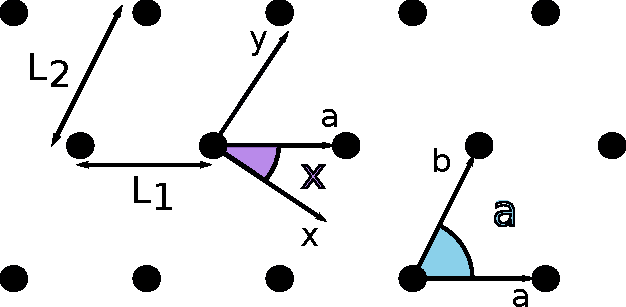
\includegraphics[width=0.5\textwidth]{fig/drawing/2Dlattice.pdf}
\end{center}
\caption{Schematic representation of a 2D lattice (top view). Such a lattice is characterized by lattice lengths $L_1$, $L_2$ and angles $\alpha$ and $\xi$.}
\label{fig:2dlattice}
\end{figure}

Like for the one-dimensional case, a probability distribution function \Code{pdf} has to be defined. One can choose between those listed in \cref{baftd} and implements it using \Code{setProbabilityDistribution(pdf)}.

\paragraph{Example} The sample used to run the simulation is made of half-spheres deposited on a substrate. The interference function is "2Dlattice" and the particles are located at the nodes of a square lattice with $L_1=L_2=20$~nm, $\v{a}\equiv \v{b}$ and the probability distribution function is Gaussian. We also use the Decoupling Approximation.

\begin{lstlisting}[language=python, style=eclipseboxed,numbers=none,nolol,caption={\Code{Python} script to define a 2DLattice interference function between hemi-spherical particles as well as the Decoupling Approximation in \Code{getSimulation()}.  The part specific to the interferences is marked in a red italic font.},label={lst:2dlatticeinterf}]
    #collection of particles
    sphere_ff = FormFactorTruncatedSphere(5*nanometer, 5*nanometer)
    sphere = Particle(m_particle, sphere_ff)
    |interference = InterferenceFunction2DLattice(20.0*nanometer, 20.0*nanometer, 90.0*degree, 0.0*degree)|
    |pdf = FTDistribution2DGauss(200.0*nanometer/2.0/M_PI, 75.0*nanometer/2.0/M_PI)|
    |interference.setProbabilityDistribution(pdf)|
    particle_layout = ParticleLayout()
    particle_layout.addParticle(sphere, 1.0)
    |particle_layout.addInterferenceFunction(interference)|

    # interference approx chosen between: DA (default) and SSCA
    |particle_layout.setApproximation(ILayout.DA)|
\end{lstlisting}

%\begin{lstlisting}[language=python, style=eclipseboxed,numbers=none,nolol]
%def get_simulation():
%    """
%    Create and return GISAXS simulation with beam and detector
%    """
%    simulation = Simulation()
%    simulation.setDetectorParameters(100, 0.0*degree, 2.0*degree, 100, 0.0*degree, 2.0*degree, True)
%    simulation.setBeamParameters(1.0*angstrom, 0.2*degree, 0.0*degree)
%    return simulation
%\end{lstlisting}


\begin{figure}[tb]
\begin{center}
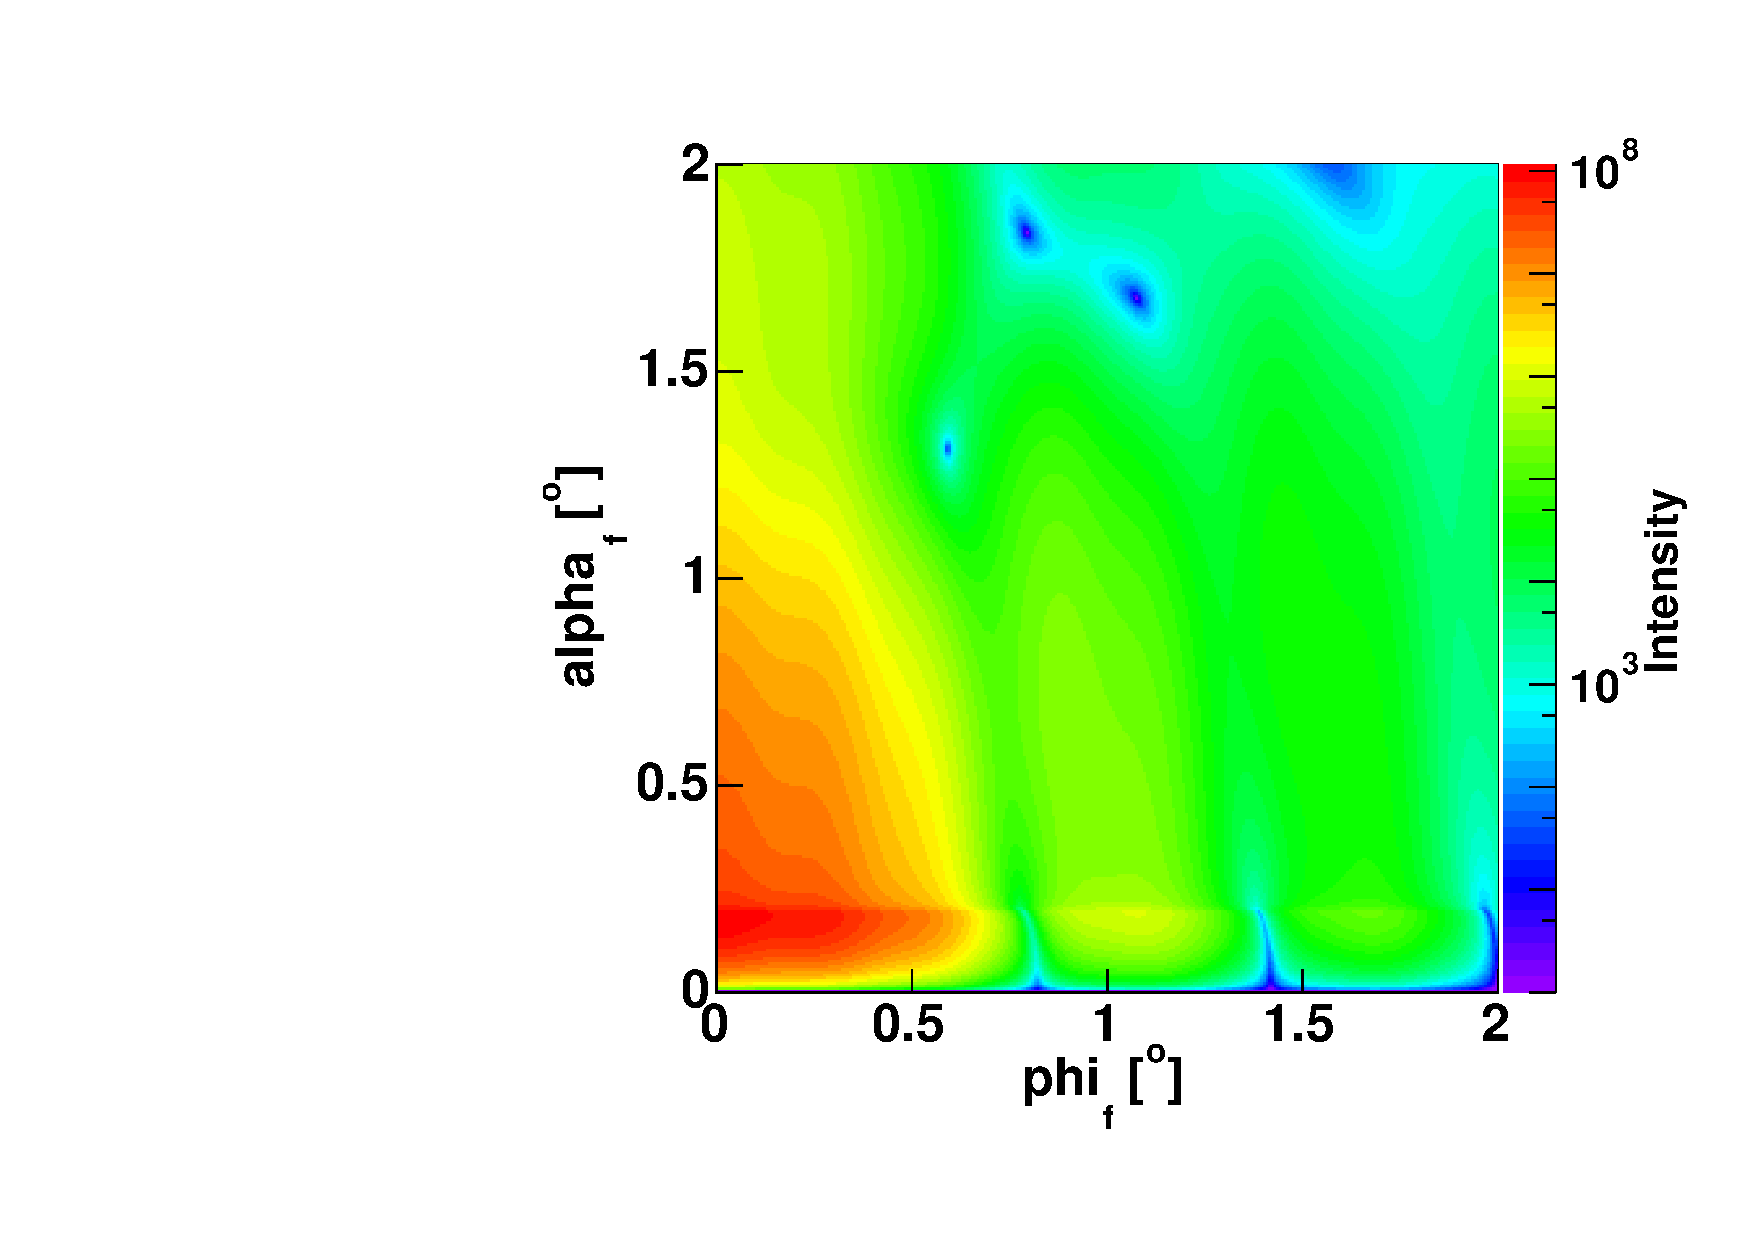
\includegraphics[angle=-90,width=0.5\textwidth]{fig/gisasmap/HSphere_2Dlattice.pdf}
\end{center}
\caption{Output intensity scattered from a sample made of half-spheres with 2DLattice interference function in the Decoupling Approximation.}
\label{fig:2dlatticeintensity}
\end{figure}

\FloatBarrier

\newpage%{\cleardoublepage}
%-------------------------------------------------------------------------------
\subsection{InterferenceFunction2DParaCrystal($L_1$, $L_2$, lattice\_angle, $xi$, damping\_length)} % TODO RESTORE \Code{}, \xi
%-------------------------------------------------------------------------------
\begin{itemize}
\item[where] $L_1$, $L_2$ are the lengths of the lattice cell,
\item[] lattice\_angle the angle between the lattice basis vectors $\v{a}, \v{b}$ in direct space,
\item[] $\xi$ is the angle defining the lattice orientation (set to $0$ by default).
\item[] \Code{damping\_length} is used to introduce finite size effects by applying a multiplicative coefficient equal to  $\exp$(-\Code{peak\_distance/damping\_length}) to the Fourier transform of the probability densities. \Code{damping\_length} is equal to 0 by default and, in this case, no correction is applied.
\end{itemize}
Two predefined interference functions can also be used:
\begin{itemize}
\item  \Code{createSquare(peak\_distance, damping\_length, domain\_size\_1, domain\_size\_2)}\\
where the angle between the base vectors of the lattice is set to $\pi/2$,
it creates a squared lattice,
\item \Code{createHexagonal(peak\_distance, damping\_length, domain\_size\_1, domain\_size\_2)}\\
where the angle between the base vectors of the lattice is set to $2\pi/3$ ,
\end{itemize}
where
\Code{domain\_size1, 2} are the dimensions of coherent domains of the paracrystal along the main axes,\\ \Code{peak\_distance} is the same in both directions and $\v{a}\equiv \v{x}$.\\

Probability distribution functions have to be defined. As the two-dimensional paracrystal is defined from two independent one-dimensional paracrystals, we need two of these functions, using\\ \Code{setProbabilityDistributions(pdf\_1, pdf\_2)}, with \Code{pdf\_{1,2}} related to each main axis of the paracrystal (see \cref{fig:2dparaschematic}).


\begin{figure}[tb]
\begin{center}
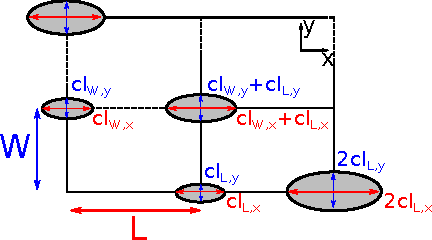
\includegraphics[width=0.75\textwidth]{fig/drawing/drawing2Dparacrystal.pdf}
\end{center}
\caption{Schematics of the ideal 2D paracrystal. The gray-shaded areas mark the regions where the probability to find a node is larger that the width at half-maximum of the distribution. $L$ and  $W$ are the mean inter-node distances along the two crystallographic axes. cl$_{(L,W),(x,y)}$ are the widths of the distribution of distance. The disorder is propagated as we add more nodes. Such a structure would be generated using \Code{InterferenceFunction2DParacrystal(L,W,90.*degrees,0,damp\_length)}, with \Code{pdf$_1$ = FTDistribution2DGauss(cl$_{L,x}$,cl$_{L,y}$)} and  \Code{pdf$_2$ = FTDistribution2DGauss(cl$_{W,x}$,cl$_{W,y}$)}.}
\label{fig:2dparaschematic}
\end{figure}


\paragraph{Example} The particles deposited on a substrate are half-spheres. The scattered beams interference via the 2DParacrystal distribution function. The paracrystal is based on a 2D hexagonal lattice with a Gaussian probability distribution function in reciprocal space.  Script~\ref{lst:2dparainterf} shows the implementation of the interference function and \cref{fig:2ddl} an example of output intensity using hemi-spherical particles.

\begin{lstlisting}[language=python, style=eclipseboxed,numbers=none,nolol,caption={\Code{Python} script to define a "2DParacrystal" interference function between particles forming an hexagonal monolayer. },label={lst:2dparainterf}]
    interference = InterferenceFunction2DParaCrystal.createHexagonal(30.0*nanometer,0.0, 40.0*micrometer, 40.0*micrometer)|
    pdf = FTDistribution2DCauchy(1.0*nanometer, 1.0*nanometer)
    interference.setProbabilityDistributions(pdf, pdf)
    particle_layout.addInterferenceFunction(interference)
\end{lstlisting}

\begin{figure}[tb]
\begin{center}
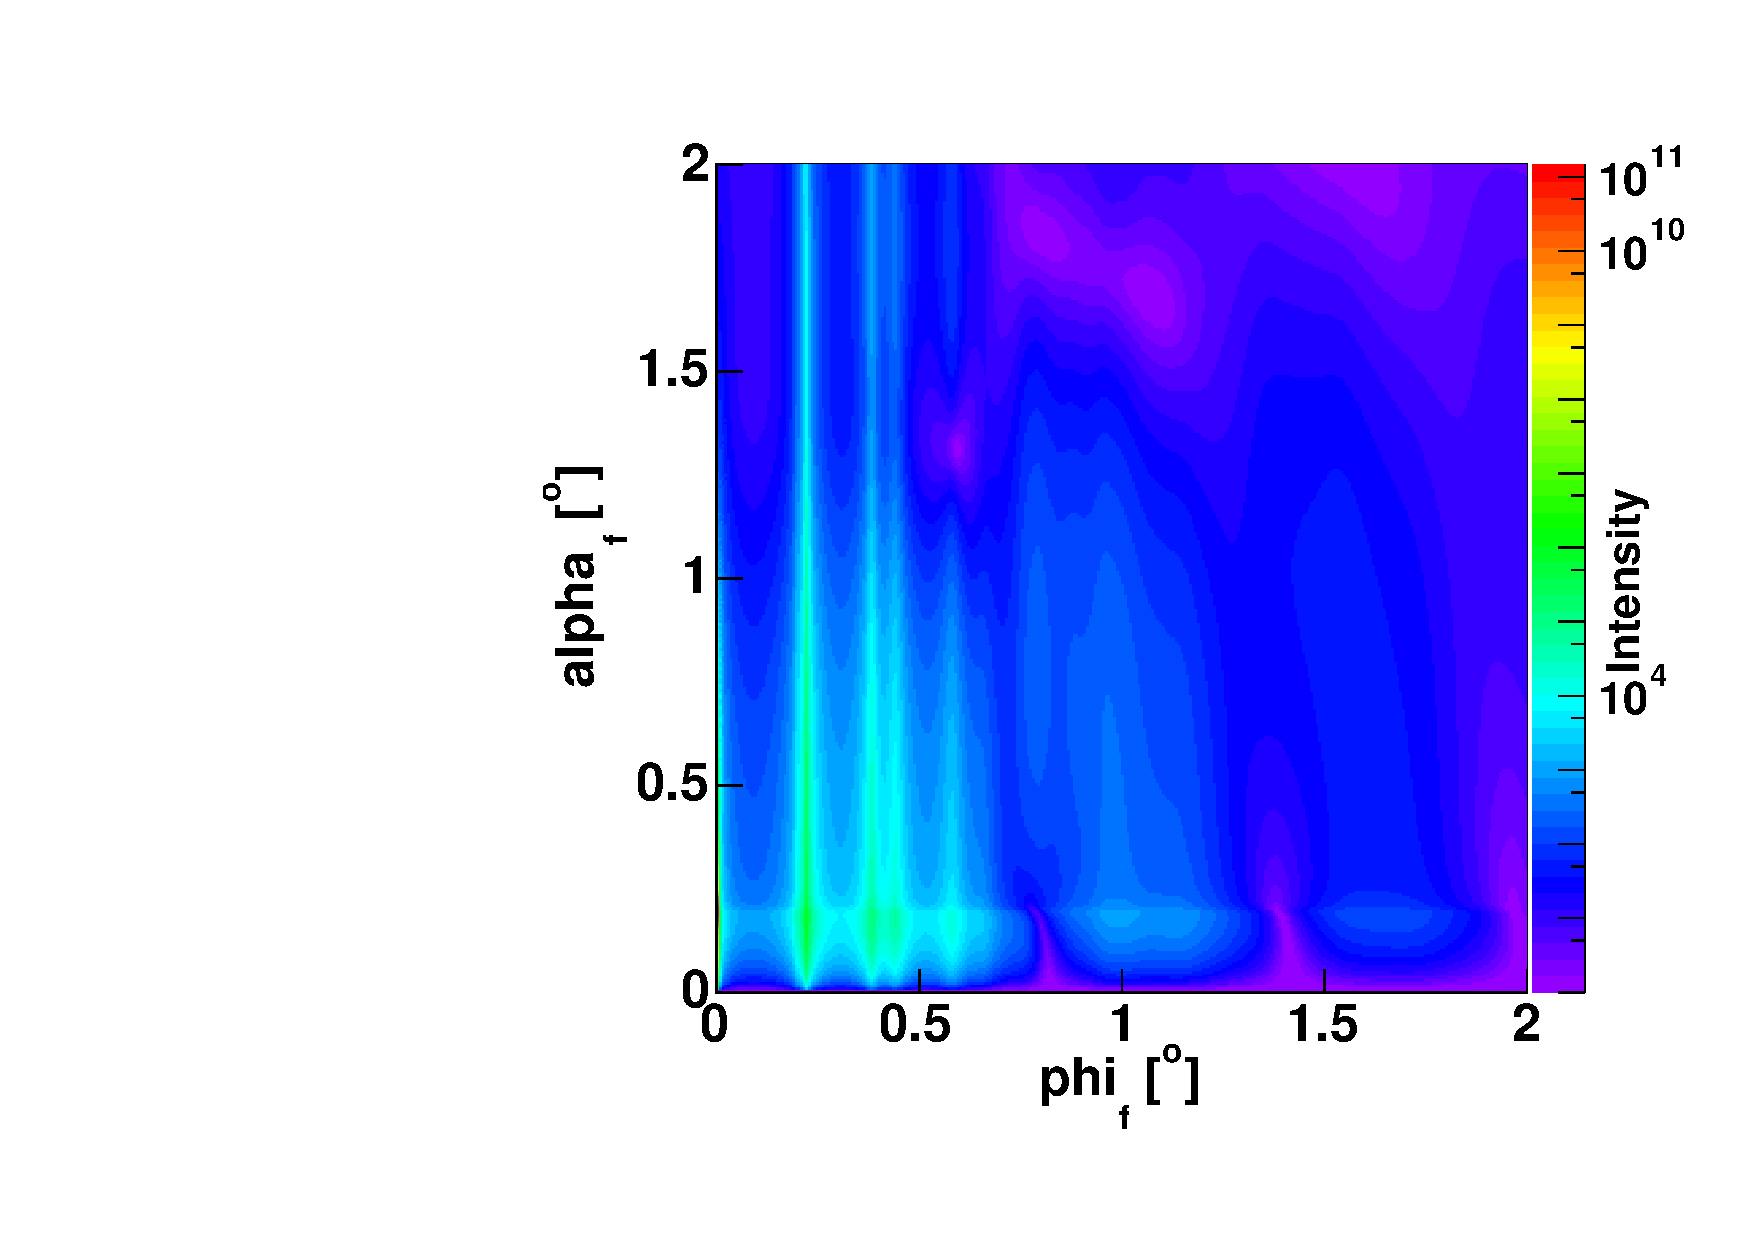
\includegraphics[angle=-90,width=0.5\textwidth]{fig/gisasmap/HSphere_2DDL.pdf}
\end{center}
\caption{Output intensity scattered from a sample made of half-spheres with 2DParacrystal interference function.}
\label{fig:2ddl}
\end{figure}

\FloatBarrier


%===============================================================================
\subsection{Summary}
%===============================================================================

\begin{table}[h]
  \footnotesize
\begin{tabular}{lll}
\hline
Function  & Parameters & Comments\\
\hline
\Code{InterferenceFunctionNone}  & None & disordered distribution \\
\hline
\Code{InterferenceFunction1DLattice} & \Code{lattice\_length} & use only with infinitely long/wide particles \\
  & $\xi=\widehat{(\v{x},\v{a})}$ & pdf=(Cauchy, Gauss or Voigt)  to be defined\\
\hline
 \Code{InterferenceFunctionRadialParaCrystal}  & peak\_distance of pdf & pdf=(Cauchy, Gauss or Voigt) to be defined \\
& damping\_length (optional) & \\
\hline
 \Code{InterferenceFunction2DLattice}  & L\_1, L\_2: lattice lengths & pdf=(Cauchy, Gauss or Voigt) to be defined\\
                        & lattice\_angle=$\widehat{(\v{a},\v{b})}$ & \\
                                                            & $\xi =\widehat{(\v{x},\v{a})}$ & \\
\hline
\Code{InterferenceFunction2DParaCrystal}  & L\_1, L\_2: lattice lengths & 2D pdf=(Cauchy, Gauss or Voigt) to be defined \\
                          & lattice\_angle=$\widehat{(\v{a},\v{b})}$ & (1 pdf per axis) \\
& $\xi=\widehat{(\v{x},\v{a})}$ & \\
& damping\_length (optional)  &  same for both axes\\
\hline
\hline
\end{tabular}
\caption{List of interference functions implemented in \BornAgain. pdf : probability distribution function, $\v{a}, \v{b}$ are the lattice base vectors, and $\v{x}$ is the axis vector perpendicular to the detector plane.}
\end{table}

\index{Particle assemblies|)}%
%\fi

%void %%%%%%%%%%%%%%%%%%%%%%%%%%%%%%%%%%%%%%%%%%%%%%%%%%%%%%%%%%%%%%%%%%%%%%%%%%%%%%%%
%%
%%   BornAgain User Manual
%%
%%   homepage:   http://www.bornagainproject.org
%%
%%   copyright:  Forschungszentrum Jülich GmbH 2015
%%
%%   license:    Creative Commons CC-BY-SA
%%   
%%   authors:    Scientific Computing Group at MLZ Garching
%%               C. Durniak, M. Ganeva, G. Pospelov, W. Van Herck, J. Wuttke
%%
%%%%%%%%%%%%%%%%%%%%%%%%%%%%%%%%%%%%%%%%%%%%%%%%%%%%%%%%%%%%%%%%%%%%%%%%%%%%%%%%


\chapter{Scattering by domain structures}  \label{sec:Domains}

\MissingSection

%void %%%%%%%%%%%%%%%%%%%%%%%%%%%%%%%%%%%%%%%%%%%%%%%%%%%%%%%%%%%%%%%%%%%%%%%%%%%%%%%%
%%
%%   BornAgain User Manual
%%
%%   homepage:   http://www.bornagainproject.org
%%
%%   copyright:  Forschungszentrum Jülich GmbH 2015
%%
%%   license:    Creative Commons CC-BY-SA
%%   
%%   authors:    Scientific Computing Group at MLZ Garching
%%               C. Durniak, M. Ganeva, G. Pospelov, W. Van Herck, J. Wuttke
%%
%%%%%%%%%%%%%%%%%%%%%%%%%%%%%%%%%%%%%%%%%%%%%%%%%%%%%%%%%%%%%%%%%%%%%%%%%%%%%%%%


\chapter{Scattering by rough interfaces}  \label{sec:Roughness}

\MissingSection

%void %%%%%%%%%%%%%%%%%%%%%%%%%%%%%%%%%%%%%%%%%%%%%%%%%%%%%%%%%%%%%%%%%%%%%%%%%%%%%%%%
%%
%%   BornAgain User Manual
%%
%%   homepage:   http://www.bornagainproject.org
%%
%%   copyright:  Forschungszentrum Jülich GmbH 2015
%%
%%   license:    Creative Commons CC-BY-SA
%%   
%%   authors:    Scientific Computing Group at MLZ Garching
%%               C. Durniak, M. Ganeva, G. Pospelov, W. Van Herck, J. Wuttke
%%
%%%%%%%%%%%%%%%%%%%%%%%%%%%%%%%%%%%%%%%%%%%%%%%%%%%%%%%%%%%%%%%%%%%%%%%%%%%%%%%%

\chapter{Modelling a GISAS experiment}  \label{sec:Exp}

To fit experimental data, it is not sufficient to simulate
the scattering of plane waves by the sample.
To account for actual detector images,
we must compute intensities in appropriate coordinates,
and account for the finite instrument resolution.

%%%%%%%%%%%%%%%%%%%%%%%%%%%%%%%%%%%%%%%%%%%%%%%%%%%%%%%%%%%%%%%%%%%%%%%%%%%%%%%%
\section{Detector images}\label{Sdetimg}
%%%%%%%%%%%%%%%%%%%%%%%%%%%%%%%%%%%%%%%%%%%%%%%%%%%%%%%%%%%%%%%%%%%%%%%%%%%%%%%%

%In this section we describe the conversion between the scattering vector~$\q$
%and the experimental coordinates.

%The experimental geometry has already been introduced in Fig.~\ref{fig:expgeom}.

\MissingSection

%%%%%%%%%%%%%%%%%%%%%%%%%%%%%%%%%%%%%%%%%%%%%%%%%%%%%%%%%%%%%%%%%%%%%%%%%%%%%%%%
\section{Instrumental resolution}\label{Sresolution}
%%%%%%%%%%%%%%%%%%%%%%%%%%%%%%%%%%%%%%%%%%%%%%%%%%%%%%%%%%%%%%%%%%%%%%%%%%%%%%%%

\MissingSection


%%%%%%%%%%%%%%%%%%%%%%%%%%%%%%%%%%%%%%%%%%%%%%%%%%%%%%%%%%%%%%%%%%%%%%%%%%%%%%%%
%%
%%   BornAgain User Manual
%%
%%   homepage:   http://www.bornagainproject.org
%%
%%   copyright:  Forschungszentrum Jülich GmbH 2016
%%
%%   license:    Creative Commons CC-BY-SA
%%
%%   authors:    Scientific Computing Group at MLZ Garching
%%               M. Ganeva, G. Pospelov, W. Van Herck, J. Wuttke
%%
%%%%%%%%%%%%%%%%%%%%%%%%%%%%%%%%%%%%%%%%%%%%%%%%%%%%%%%%%%%%%%%%%%%%%%%%%%%%%%%%

\newpage
\chapter{The three interfaces of \BornAgain}  \label{sec:API3}

%%%%%%%%%%%%%%%%%%%%%%%%%%%%%%%%%%%%%%%%%%%%%%%%%%%%%%%%%%%%%%%%%%%%%%%%%%%%%%%%
\section{Architectural overview}
%%%%%%%%%%%%%%%%%%%%%%%%%%%%%%%%%%%%%%%%%%%%%%%%%%%%%%%%%%%%%%%%%%%%%%%%%%%%%%%%

The overall architecture of \BornAgain\ is outlined in \cref{Farch1}.
The core of \BornAgain\
\index{Core|see {\Code{libBornAgainCore}}}
comprises functionality to construct arbitrary hierarchical sample models,
to setup instrument models,
and to compute the expected detector image for any given sample and instrument model.
Furthermore \BornAgain\ comes with various minimizers that optimize model parameters
to fit the simulated detector image to a given experimental image.
All this functionality is implemented in a library, \Code{libBornAgainCore}.

\begin{figure}[tbh]
\begin{center}
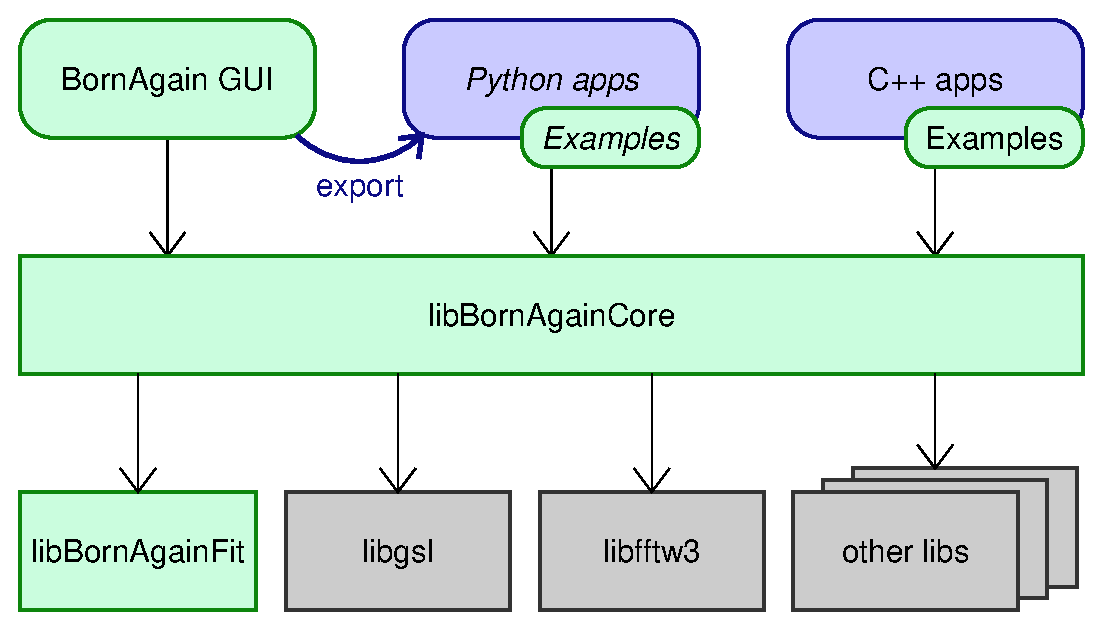
\includegraphics[width=0.8\textwidth]{fig/drawing/architecture1.ps}
\end{center}
\caption{Overall architecture of \BornAgain.
\index{Architecture!applications and libraries}%
Applications are shown as oval fields, libraries as rectangles.
Green fields designate software that is part of \BornAgain.
Gray fields are external dependences
(only two external libraries are explicitly shown;
several more are listed in the online compilation instructions).
Blue fields indicate stand-alone applications that use \BornAgain's
two Application Programming Interfaces (the C$++$ API and the Python API).
\index{C++!using BornAgain from}
\index{Python!using BornAgain from}
\index{Application Programming Interface}
While such applications are to be written by users,
some examples come with the \BornAgain\ source distribution,
and are explained in the following Manual chapters.
It is also possible to export a simulation setup from GUI as Python code.}
\label{Farch1}
\end{figure}

\index{libBornAgainCore@\Code{libBornAgainCore}}
This library, in turn, depends on a number of other libraries.
One of these, the minimizer wrapper \Code{libBornAgainFit}
\index{libBornAgainFit@\Code{libBornAgainFit}}
\index{Minimizers|see \Code{libBornAgainFit}}
has been written specifically for use in \BornAgain,
and for the time being is only distributed as part of \BornAgain,
though in the future it may find applications in other contexts.
The other library dependences of \Code{libBornAgainCore}
are multi-purpose libraries that are easily available as open-source packages.
\index{Dependences!libraries}

The library \Code{libBornAgainCore} can be used in three different ways:
From its graphical user interface (GUI), or
from user-written stand-alone applications in the programming languages C$++$ or Python.
These different approaches are briefly outlined below.
The Python interface is then described at length in the next chapters.

%%%%%%%%%%%%%%%%%%%%%%%%%%%%%%%%%%%%%%%%%%%%%%%%%%%%%%%%%%%%%%%%%%%%%%%%%%%%%%%%
\section{Using \BornAgain\ from its Graphical User Interface}
%%%%%%%%%%%%%%%%%%%%%%%%%%%%%%%%%%%%%%%%%%%%%%%%%%%%%%%%%%%%%%%%%%%%%%%%%%%%%%%%
\index{Graphical User Interface|(}
\index{bornagain@\Code{bornagain}|see {Graphical User Interface}}
\index{Exectutable!bornagain@\Code{bornagain}|see {Graphical User Interface}}
\index{Binary|see {Executable}}
%\index{Project name!BornAgain@\BornAgain}

The project \BornAgain\ comes with a stand-alone application called \Code{bornagain}
that provides a Graphical User Interface (GUI).
Note that we distinguish between the GUI executable \Code{bornagain},
the underlying library \Code{libBornAgainCore}, and the project \BornAgain\ at large.

The GUI allows users to quickly setup a simulation, to visualize simulated
detector images, to compare with experimental images, and to run fits.
It provides comfortable access to much, but not all the functionality
of \Code{libBornAgainCore}.
Depending on application fields,
users may sooner or later reach the limits of current GUI support.
Other users may have repetitive tasks that are cumbersome under a GUI.
In such cases, users can export their sample and instrument models from
the GUI as a Python script,
and continue work by directly editing the Python code.
\index{Export!Python from GUI}

\Link{Documentation of the GUI is available online:\\
      \url{http://www.bornagainproject.org/documentation/usage/gui}}
\index{Graphical User Interface|)}

%%%%%%%%%%%%%%%%%%%%%%%%%%%%%%%%%%%%%%%%%%%%%%%%%%%%%%%%%%%%%%%%%%%%%%%%%%%%%%%%
\section{Using \BornAgain\ from Python}
%%%%%%%%%%%%%%%%%%%%%%%%%%%%%%%%%%%%%%%%%%%%%%%%%%%%%%%%%%%%%%%%%%%%%%%%%%%%%%%%
\index{Python!using BornAgain from|(}

\BornAgain\ simulations and fits can be set up and run from Python scripts
or from a Python command line.

\index{Python!using BornAgain from|)}

%%%%%%%%%%%%%%%%%%%%%%%%%%%%%%%%%%%%%%%%%%%%%%%%%%%%%%%%%%%%%%%%%%%%%%%%%%%%%%%%
\section{Using \BornAgain\ from C++}
%%%%%%%%%%%%%%%%%%%%%%%%%%%%%%%%%%%%%%%%%%%%%%%%%%%%%%%%%%%%%%%%%%%%%%%%%%%%%%%%
\index{C++!using BornAgain from|(}

The library \Code{libBornAgainCore}
\index{libBornAgainCore@\Code{libBornAgainCore}}%
\index{C++!libBornAgainCore@{\Code{libBornAgainCore} written in}}%
is written in the programming languages C++,
and therefore natively supports usage from application programs written in C++.

\index{C++!using BornAgain from|)}

%%%%%%%%%%%%%%%%%%%%%%%%%%%%%%%%%%%%%%%%%%%%%%%%%%%%%%%%%%%%%%%%%%%%%%%%%%%%%%%%
%%
%%   BornAgain User Manual
%%
%%   homepage:   http://www.bornagainproject.org
%%
%%   copyright:  Forschungszentrum Jülich GmbH 2015
%%
%%   license:    Creative Commons CC-BY-SA
%%
%%   authors:    Scientific Computing Group at MLZ Garching
%%               C. Durniak, M. Ganeva, G. Pospelov, W. Van Herck, J. Wuttke
%%
%%%%%%%%%%%%%%%%%%%%%%%%%%%%%%%%%%%%%%%%%%%%%%%%%%%%%%%%%%%%%%%%%%%%%%%%%%%%%%%%


\newpage
\chapter{Using the Python API}  \label{sec:Usage}


%%%%%%%%%%%%%%%%%%%%%%%%%%%%%%%%%%%%%%%%%%%%%%%%%%%%%%%%%%%%%%%%%%%%%%%%%%%%%%%%
\section{Running a simulation}
%%%%%%%%%%%%%%%%%%%%%%%%%%%%%%%%%%%%%%%%%%%%%%%%%%%%%%%%%%%%%%%%%%%%%%%%%%%%%%%%

A simulation of GISAS using \BornAgain\ consists of the following steps:
\begin{itemize}
\item define materials by specifying name and refractive index,
\item define layers by specifying thickness, roughness, material,
\item define embedded particles by specifying shape, size,
   constituting material, interference function,
\item embed the particles in layers, specifying density, position, orientation,
\item assemble a multilayered sample,
\item specify input beam and detector characteristics,
\item run the simulation,
\item save the simulated detector image.
\end{itemize}

\noindent
All these steps can be organized in either a Graphical User Interface (GUI) or by providing a Python script with the simulation description.
In the following, we describe how to write a
\Code{Python} script which runs a \BornAgain\ simulation. For tutorials about this programming language, the users are referred to \cite{Lut09}.


% More information about the general software architecture and \BornAgain\ internal design are given in \cref{sec:SoftwareArchitecture}.


%===============================================================================
\subsection{Units:}
%===============================================================================
\index{Units}

By default the angles are expressed in radians and the lengths are given in
nanometers.  But it is possible to use other units by
specifying them right after the value of the corresponding
parameter like, for example, \Code{20.0*micrometer}.


%===============================================================================
\subsection{A first example} \label{sec:Example1Python}
%===============================================================================

In this example, we simulate the scattering from a mixture of
cylindrical and prismatic nanoparticles without any interference
between them. These particles are placed in air, on top
of a substrate.\\ We are going to go through each step of the
simulation. The \Python\ code snippet specific to each stage will be given at
the beginning of the description.
More examples can be found at our project web site \url{http://www.bornagainproject.org/documentation/python_examples}

% But for the sake of completeness the full code is given
% in Appendix~\ref{PythonSimulationExampleScript}.

%-------------------------------------------------------------------------------
\subsubsection{Importing Python modules}
%-------------------------------------------------------------------------------

\begin{lstlisting}[language=python, style=eclipseboxed,name=ex1,nolol]
import numpy @\label{import_lib_beg}@
import matplotlib
import pylab @\label{import_lib_end}@
from bornagain import * @\label{import_ba}@
\end{lstlisting}
We start by importing different functions from external
modules, for example \Code{NumPy} (lines~\ref{import_lib_beg}-\ref{import_lib_end}), which
is a fundamental package for scientific computing with \Python\
\cite{s:numpy}.  In particular, line~\ref{import_ba}
imports the features of \BornAgain\ software.

%-------------------------------------------------------------------------------
\subsubsection{Defining the materials}
%-------------------------------------------------------------------------------

\begin{lstlisting}[language=python, style=eclipseboxed,name=ex1,nolol]
def get_sample(): @\label{def_function}@
    """
    Build and return the sample representing cylinders and pyramids on top of substrate without interference.
   """
    # defining materials @\label{material1}@
    m_air = HomogeneousMaterial("Air", 0.0, 0.0)  @\label{material2}@
    m_substrate = HomogeneousMaterial("Substrate", 6e-6, 2e-8) @\label{material3}@
    m_particle = HomogeneousMaterial("Particle", 6e-4, 2e-8) @\label{materialparticle}@

\end{lstlisting}
Line~\ref{def_function} marks the beginning of the
function to define our sample. Lines~\ref{material2}, \ref{material3} and \ref{materialparticle} define different
materials using class \Code{HomogeneousMaterial}. The general syntax is the following
\begin{lstlisting}[language=python, style=eclipse,numbers=none]
<material_name> = HomogeneousMaterial("name", delta, beta)
\end{lstlisting}
where \Code{name} is the name of the
material associated with its complex refractive index
n=1-\Code{delta} +i \Code{beta}. \Code{<material\_name>} is later used when
referring to this particular material. The three materials defined in this example are \Code{Air} with a refractive
index of 1 (\Code{delta = beta = 0}), a \Code{Substrate} associated with a complex refractive index
equal to $1-6\times 10^{-6} +i2\times 10^{-8} $, and the material of the particles, whose refractive index is \Code{n}$=1-6\times 10^{-4}+i2\times 10^{-8}$.

%-------------------------------------------------------------------------------
\subsubsection{Defining the particles}
%-------------------------------------------------------------------------------
\begin{lstlisting}[language=python,style=eclipseboxed,name=ex1,nolol]
    # collection of particles @\label{particles1}@
    cylinder_ff = FormFactorCylinder(5*nanometer, 5*nanometer) @\label{particlescyl1}@
    cylinder = Particle(m_particle, cylinder_ff) @\label{particlescyl2}@
    prism_ff = FormFactorPrism3(10*nanometer, 5*nanometer) @\label{particlesprism1}@
    prism = Particle(m_particle, prism_ff) @\label{particlesprism2}@
\end{lstlisting}
We implement two different shapes of particles: cylinders and
prisms (\idest  elongated particles with a constant equilateral triangular cross section).

All particles implemented in \BornAgain\ are defined by their
form factors (see Appendix~\ref{app:ff}), their sizes and the material
they are made of. Here, for the
cylindrical particle, we input its radius and height.  For the prism,
the possible inputs are the length of one side of its equilateral triangular
base and its height.

In order to define a particle, we proceed in two steps. For example for
the cylindrical particle, we first specify the form factor of a cylinder with
its radius and height, both equal to 5 nanometers in this particular
case (see line~\ref{particlescyl1}). Then we associate this shape with
the constituting material as in line~\ref{particlescyl2}.
The same procedure has been applied for the prism in lines~\ref{particlesprism1} and \ref{particlesprism2}, respectively.

%-------------------------------------------------------------------------------
\subsubsection{Characterizing particles assembly}
%-------------------------------------------------------------------------------
\begin{lstlisting}[language=python, style=eclipseboxed, name=ex1,nolol]
    particle_layout = ParticleLayout()  @\label{particlesdecor1}@
    particle_layout.addParticle(cylinder, 0.5)  @\label{particlesdecor2}@
    particle_layout.addParticle(prism, 0.5)@\label{particlesdecor3}@
    interference = InterferenceFunctionNone()  @\label{particlesnointerf}@
    particle_layout.addInterferenceFunction(interference)  @\label{particlesinterf}@
\end{lstlisting}
The object which holds the information about the positions and densities of particles
in our sample is called \Code{ParticleLayout}
(line~\ref{particlesdecor1}). We use the associated function \Code{addParticle}
for each particle shape (lines~\ref{particlesdecor2}, \ref{particlesdecor3}). Its general syntax is

\begin{lstlisting}[language=python, style=eclipse,numbers=none]
addParticle(<particle_name>, abundance)
\end{lstlisting}
where \Code{<particle\_name>} is the name used to define the particles
(lines~\ref{particlescyl2} and \ref{particlesprism2}) and
\Code{abundance} is the proportion of this type of particles,
normalized to the total number of particles. Here we have 50\% of cylinders
and 50\% of prisms.

\noindent Finally, lines~\ref{particlesnointerf} and
\ref{particlesinterf} specify that there is \textbf{no coherent interference} between
the waves scattered by these particles. In this case, the intensity is calculated by
the incoherent sum of the scattered waves: $\bra |F_j|^2\ket$,
where $F_j$ is the form factor associated with the particle of type $j$.  The way these waves
interfere imposes the horizontal distribution of
the particles as
the interference reflects the long or short-range order of the
particles distribution (see  \cref{sec:sect:interf}). On the contrary, the vertical position is
imposed when we add the particles in a given layer by parameter \Code{depth}, as shown in lines~\ref{particlesdecor2} and \ref{particlesdecor3}.

%-------------------------------------------------------------------------------
\subsubsection{Multilayer}
%-------------------------------------------------------------------------------
\begin{lstlisting}[language=python, style=eclipseboxed,name=ex1,nolol]
# air layer with particles and substrate form multi layer  @\label{sampleassembling}@
    air_layer = Layer(m_air) @\label{airlayer}@
    air_layer.addLayout(particle_layout) @\label{airlayerdecorator}@
    substrate_layer = Layer(m_substrate, 0)  @\label{substratelayer}@
    multi_layer = MultiLayer() @\label{multilayercanvas}@
    multi_layer.addLayer(air_layer) @\label{layerairdecor}@
    multi_layer.addLayer(substrate_layer) @\label{layersubstrate}@
    return multi_layer @\label{returnmlayer}@
\end{lstlisting}
We now have to configure our sample. For this first example,
the particles, \idest  cylinders and prisms, are on top of a substrate in an
air layer. \textbf{The order in which we define these layers is important: we
start from the top layer down to the bottom one}.

Let us start with the air layer. It contains the particles. In
line~\ref{airlayer}, we use the previously defined \Code{m\_air}
(="air" material) (line~\ref{material2}). The command in line~\ref{airlayerdecorator} shows that this layer contains particles
which are defined using particle layout object. The substrate layer
only contains the substrate material (line~\ref{substratelayer}).
%Note that the
%\Code{depth} is referenced to the bottom of the top layer (negative
%values would correspond to particles floating above layer 1 as
%the vertical axis is pointing upwards).

There are different possible syntaxes to define a layer. As shown in
lines~\ref{airlayer} and \ref{substratelayer}, we can use
\Code{Layer(<material\_name>,thickness)} or
\Code{Layer(<material\_name>)}. The second case corresponds
to the default value of the \Code{thickness}, equal to 0. The \Code{thickness} is
expressed in  nanometers.

Our two layers are now fully characterized. The sample is assembled using
\Code{MultiLayer()} constructor (line~\ref{multilayercanvas}): we start with the air layer decorated
with the particles (line~\ref{layerairdecor}), which is the layer at
the top and end with the bottom layer, which is the
substrate (line~\ref{layersubstrate}).

%-------------------------------------------------------------------------------
\subsubsection{Characterizing the input beam and output detector}
%-------------------------------------------------------------------------------

\begin{lstlisting}[language=python, style=eclipseboxed,name=ex1,nolol]
def get_simulation():  @\label{run1}@
    """
    Create and return GISAXS simulation with beam and detector defined
    """
    simulation = Simulation() @\label{run2}@
    simulation.setDetectorParameters(100, -1.0*degree, 1.0*degree, 100, 0.0*degree, 2.0*degree) @\label{rundetector}@
    simulation.setBeamParameters(1.0*angstrom, 0.2*degree, 0.0*degree) @\label{runbeam}@
    return simulation @\label{returnsimul}@
\end{lstlisting}
The first stage is to create the \Code{Simulation()} object (line~\ref{run2}). Then we define the detector (line~\ref{rundetector}) and beam
parameters (line~\ref{runbeam}). %, which are associated with the
%sample previously defined (line~\ref{runsample}). Finally we run
%the simulation (line~\ref{runsimul}).
Those functions are part of the Simulation
class.  The different incident and exit angles are
shown in \cref{fig:multil3d}.

The detector parameters are set using ranges of angles via
the function:

\begin{lstlisting}[language=python, style=eclipse,numbers=none]
setDetectorParameters(n_phi, phi_f_min, phi_f_max, n_alpha, alpha_f_min, alpha_f_max),
\end{lstlisting}


\noindent where number of bins \Code{n\_phi}, low edge of first bin \Code{phi\_f\_min} and
upper edge of last bin \Code{phi\_f\_max} all together define $\phi_f$ detector axis,
while \Code{n\_alpha}, \Code{alpha\_f\_min} and \Code{alpha\_f\_max} are related to
$\alpha_f$ detector axis.

\ImportantPoint{Remark:}{Axis binning\\
By default axes are binned to provide constant bin size in k-space, which means slightly
non-equidistant binning in angle space. Other possible options, including user defined
axes with custom variable bin size are explained elsewhere.
}
\vspace*{2mm}

%are the minimum and maximum values of $\phi_f$, respectively, \Code{n\_alpha} is
%the number of bins for $\alpha_f$ axis, \Code{alpha\_f\_min} and \Code{alpha\_f\_max}
%are the minimum and maximum values of
%$\alpha_f$, respectively.

%\Code{isgisaxs\_style=True} (default value = \Code{False}) is a boolean
%used to characterise the structure of the output data. If
%\Code{isgisaxs\_style=True}, the output data is binned at constant
%values of the sine of the output angles, $\alpha_f$ and $\phi_f$, otherwise it is binned
%at constant values of these two angles.\\

\noindent To characterize the beam we use function
\begin{lstlisting}[language=python, style=eclipse,numbers=none]
setBeamParameters(lambda, alpha_i, phi_i),
\end{lstlisting}

\noindent where \Code{lambda} is the incident beam wavelength,
\Code{alpha\_i} is the incident
grazing angle on the surface of the sample,
\Code{phi\_i} is the in-plane
direction of the incident beam (measured with respect to the $x$-axis).


%-------------------------------------------------------------------------------
\subsubsection{Running the simulation and plotting the results}
%-------------------------------------------------------------------------------

\begin{lstlisting}[language=python, style=eclipseboxed,name=ex1,nolol]
def run_simulation(): @\label{run_simulation}@
    """
   Run simulation and plot results
    """
    sample = get_sample() @\label{get_sample}@
    simulation = get_simulation() @\label{get_simulation}@
    simulation.setSample(sample)  @\label{setsample}@
    simulation.runSimulation()  @\label{runsimul}@
    result = simulation.getIntensityData().getArray() + 1  # for log scale  @\label{outputdata}@
    pylab.imshow(numpy.rot90(result, 1), norm=matplotlib.colors.LogNorm(), extent=[-1.0, 1.0, 0, 2.0]) @\label{plot1}@
    pylab.show() @\label{plot2}@
\end{lstlisting}
%In function \Code{run\_simulation()}, we associate the sample
%characterised by function \Code{get\_sample()} with the input beam and
%output detector, defined in function \Code{get\_simulation()} (line~\ref{runsample}).
The function, whose definition starts from line~\ref{run_simulation}, gathers all
items. We create the sample and the simulation objects at the lines
~\ref{get_sample} and \ref{get_simulation}, using calls to the previously defined functions. We assign the sample to the simulation at line ~\ref{setsample} and
finally launch the simulation at line ~\ref{runsimul}.

In line~\ref{outputdata} we obtain the simulated intensity
as a function of outgoing angles $\alpha_f$ and $\phi_f$ for further
uses (plots, fits,\ldots) as a \Code{NumPy} array containing
\Code{n\_phi}$\times$\Code{n\_alpha}
datapoints. Lines~\ref{plot1}-\ref{plot2} produces the two-dimensional
contour plot of the intensity as a function of $\alpha_f$ and
$\phi_f$ shown in \cref{fig:output_ex1}.

\begin{figure}[htbp]
  \begin{center}
   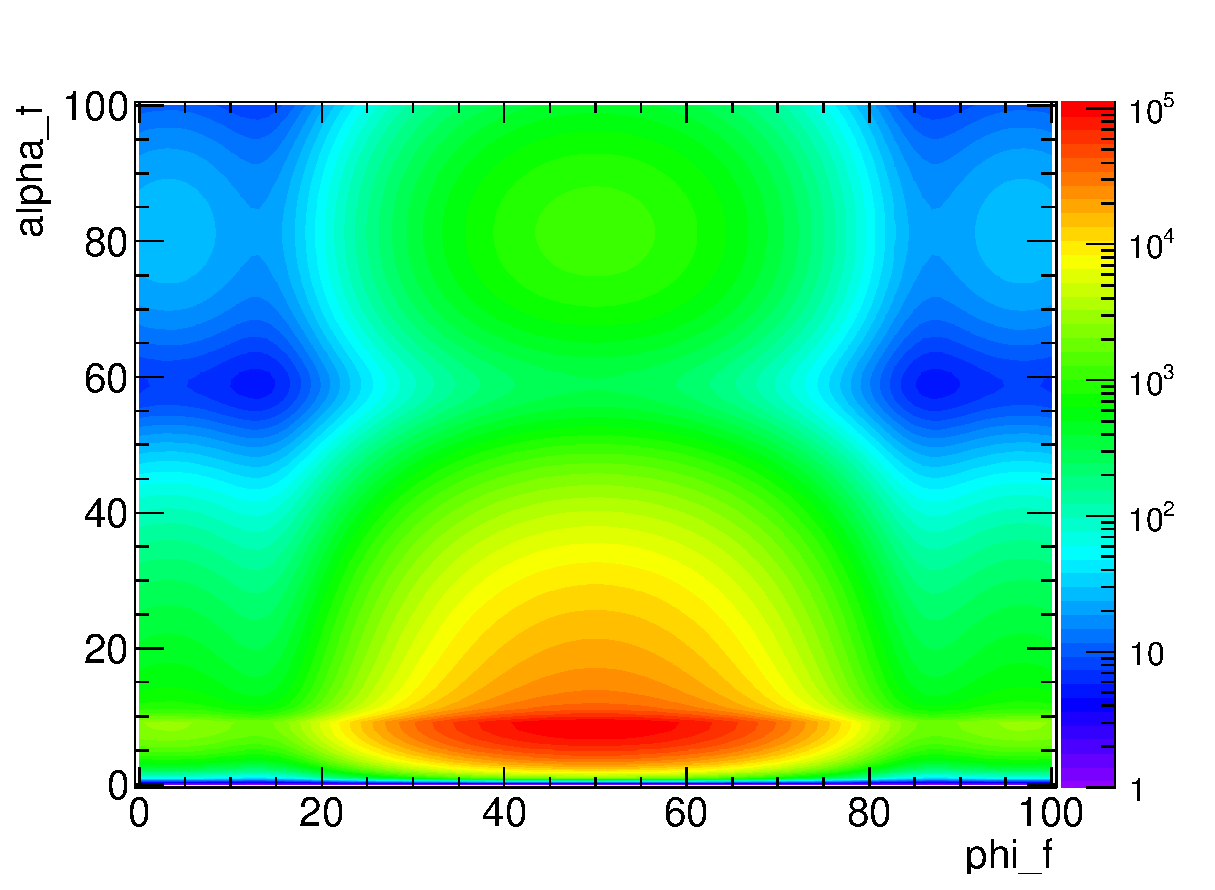
\includegraphics[clip=true, width=120mm]{fig/gisasmap/Manual_ex1.eps}
  \end{center}
  \caption[Example 1: Simulated grazing-incidence small-angle X-ray scattering from a mixture of
cylindrical and prismatic nanoparticles without any interference, deposited on top
of a substrate]{Simulated grazing-incidence small-angle X-ray scattering from a mixture of
cylindrical and prismatic nanoparticles without any interference, deposited on top
of a substrate. The input beam is characterized by a wavelength
$\lambda$ of 1~\AA\ and incident angles $\alpha_i=0.2^{\circ}$, $\phi_i=0^{\circ}$. The
cylinders have a radius and a height both equal to 5~nm, the prisms
are characterized by a side length equal to 10~nm and they are 5~nm high. The
material of the particles has a refractive index of $1-6\times 10^{-4}+i2\times 10^{-8}$. For the substrate
it is equal to $1-6\times 10^{-6} +i2\times 10^{-8} $. The color scale
is associated with the output intensity in arbitrary units. }
\label{fig:output_ex1}
\end{figure}


%===============================================================================
\subsection{Working with sample parameters}
   \label{sec:WorkingWithSampleParameters}
%===============================================================================


This section gives additional details about the manipulation of sample parameters
during run time; that is after the sample has already been constructed.
For a single simulation this is normally not necessary. However it might be useful
during interactive work when the user tries to find optimal sample parameters by
running a series of simulations.
A similar task also arises when the theoretical model, composed of the
description of the sample and of the simulation, is used for fitting real data.
In this case, the fitting kernel requires a list of the existing sample parameters
and a mechanism for changing the values of these parameters in order to find
their optima.

In \BornAgain\ this is done using the so-called sample parameter pool
mechanism. We are going to briefly explain this approach using the example
of \cref{sec:Example1Python}.

In \BornAgain\ a sample is described by a hierarchical tree of objects.
For the multilayer created in the previous section this tree can be graphically
represented as shown in \cref{fig:sample_tree}. Similar trees can
be printed in a \Python\
session by running \Code{multi\_layer.printSampleTree()}

\begin{figure}[p!]

\tikzstyle{every node}=[draw=black,thick,anchor=west]
\tikzstyle{selected}=[draw=red,fill=red!30]
\tikzstyle{optional}=[dashed,fill=gray!50]
\begin{tikzpicture}[%
  grow via three points={one child at (0.5,-0.7) and
  two children at (0.5,-0.7) and (0.5,-1.4)},
  edge from parent path={(\tikzparentnode.south) |- (\tikzchildnode.west)}]
  \node {MultiLayer}
    child { node {Layer \#0}
		child { node {ParticleLayout }
			child { node {Particle Info 0}
				child {node {Particle }
					child { node {FormFactorCylinder}
						child { node [optional] { radius:5.0} }
						child { node [optional] { height:5.0} }
					}
				}
    			child [missing] {}
    			child [missing] {}
			    child [missing] {}
				child {node [optional] { abundance:0.5} }
				child {node [optional] { depth:0.0} }
			}
    		child [missing] {}
    		child [missing] {}
			child [missing] {}
    		child [missing] {}
    		child [missing] {}
			child [missing] {}
			child { node {Particle Info 1}
				child {node {Particle }
					child { node {FormFactorPrism3}
						child { node [optional] { length:10.0} }
						child { node [optional] { height:5.0} }
					}
				}
    			child [missing] {}
    			child [missing] {}
			    child [missing] {}
				child {node [optional] { abundance:0.5} }
				child {node [optional] { depth:0.0} }
			}
		}
		child [missing] {}
   		child [missing] {}
	    child [missing] {}
		child [missing] {}
   		child [missing] {}
	    child [missing] {}
	    child [missing] {}
		child [missing] {}
   		child [missing] {}
	    child [missing] {}
		child [missing] {}
   		child [missing] {}
	    child [missing] {}
	    child [missing] {}
		child {node [optional] { thickness:0.0} }
    }
	child [missing] {}
   	child [missing] {}
	child [missing] {}
   	child [missing] {}
	child [missing] {}
	child [missing] {}
   	child [missing] {}
	child [missing] {}
   	child [missing] {}
	child [missing] {}
	child [missing] {}
   	child [missing] {}
	child [missing] {}
   	child [missing] {}
	child [missing] {}
	child [missing] {}
	child { node {Layer interface \#0}
    	child {node { roughness}
    		child {node [optional] { corrlength:0.0} }
    		child {node [optional] { hurst:0.0} }
    		child {node [optional] { sigma:0.0} }
    	}
	}
   	child [missing] {}
	child [missing] {}
	child [missing] {}
    child { node {Layer \#1}
    	child {node [optional] { thickness:0.0} }
    }
	child [missing] {}
    child { node [optional] {CrossCorrLength:0.0} };

\end{tikzpicture}
\caption{Tree representation of the sample structure.}
\label{fig:sample_tree}
\end{figure}


The top \Code{MultiLayer} object is composed of three children, namely
\Code{Layer \#0, Layer Interface \#0} and \Code{Layer \#1}. The
children objects might themselves also be decomposed into tree-like structures. For example,
\Code{Layer \#0} contains a \Code{ParticleLayout} object, which holds information
related to the two types of particles populating the layer. All numerical values used
during the sample construction (thickness of layers, size of particles, roughness parameters) are part of the same tree structure.
They are marked in the figure with shaded gray boxes.

These values are registered in the sample parameter pool using the name
composed of the corresponding nodes' names. And they can be accessed/changed
during run time. For example, the \Code{height} of the cylinders
populating the first layer can be changed from the
current value of $5~\rm{nm}$ to $1~\rm{nm}$ by running the command

\begin{lstlisting}[language=shell, style=commandline]
multi_layer.setParameterValue('/MultiLayer/Layer0/ParticleLayout/ParticleInfo0/Particle/FormFactorCylinder/height', 1.0)
\end{lstlisting}


A list of the names and values of all registered sample's parameters
can be displayed using the command

\begin{lstlisting}[language=shell, style=commandline]
> multi_layer.printParameters()
The sample contains following parameters ('name':value)
'/MultiLayer/Layer0/ParticleLayout/ParticleInfo0/Particle/FormFactorCylinder/height':5
'/MultiLayer/Layer0/ParticleLayout/ParticleInfo0/Particle/FormFactorCylinder/radius':5
'/MultiLayer/Layer0/ParticleLayout/ParticleInfo0/abundance':0.5
'/MultiLayer/Layer0/ParticleLayout/ParticleInfo0/depth':0
'/MultiLayer/Layer0/ParticleLayout/ParticleInfo1/Particle/FormFactorPrism3/length':5
'/MultiLayer/Layer0/ParticleLayout/ParticleInfo1/Particle/FormFactorPrism3/height':5
'/MultiLayer/Layer0/ParticleLayout/ParticleInfo1/abundance':0.5
'/MultiLayer/Layer0/ParticleLayout/ParticleInfo1/depth':0
'/MultiLayer/Layer0/thickness':0
'/MultiLayer/Layer1/thickness':0
'/MultiLayer/LayerInterface/roughness/corrlength':0
'/MultiLayer/LayerInterface/roughness/hurst':0
'/MultiLayer/LayerInterface/roughness/sigma':0
'/MultiLayer/crossCorrLength':0
\end{lstlisting}

Wildcards \Code{'*'} can be used to reduce typing or to work on a group
of parameters. In the example below, the first command will change the
height of all cylinders in the same way, as in the previous example. The second line will change simultaneously the height of {\it both} cylinders and prisms.
\begin{lstlisting}[language=shell, style=commandline]
multi_layer.setParameterValue('*FormFactorCylinder/height', 1.0)
multi_layer.setParameterValue('*height', 1.0)
\end{lstlisting}

The complete example described in this section can be found at
\begin{lstlisting}[language=shell, style=commandline]
./Examples/python/fitting/ex001_SampleParametersIntro/SampleParametersIntro.py
\end{lstlisting}

%%%%%%%%%%%%%%%%%%%%%%%%%%%%%%%%%%%%%%%%%%%%%%%%%%%%%%%%%%%%%%%%%%%%%%%%%%%%%%%%
\section{Fitting} \label{sec:Fitting}
%%%%%%%%%%%%%%%%%%%%%%%%%%%%%%%%%%%%%%%%%%%%%%%%%%%%%%%%%%%%%%%%%%%%%%%%%%%%%%%%
  \index{Fitting|(}

In addition to the simulation of grazing incidence
X-ray and neutron scattering by
multilayered samples, \BornAgain\ also offers the option to
fit the numerical model to reference data by modifying a selection of
sample parameters from the numerical model.  This aspect
of the software is discussed in the current chapter.

%\cref{sec:FittingGentleIntroducion} gives a short introduction to the
%basic concepts of data fitting. Users familiar with fitting can
%directly proceed to \cref{sec:FittingImplementation}, which details the
%implementation of fittings in
%\BornAgain\ .
\cref{sec:FittingImplementation} details the
implementation of fittings in \BornAgain\ .
\Python\ fitting examples with detailed
explanations of every fitting step are given in \cref{sec:FittingExamples}. Advanced fitting techniques, including fine tuning of minimization
algorithms, simultaneous fits of different data sets, parameters
correlation, are covered in
\cref{sec:FittingAdvanced}. \cref{sec:FittingRightAnswers} contains some practical advice, which might
help the user to get right answers from \BornAgain\ fitting.


\subsubsection{Implementation in BornAgain} \label{sec:FittingImplementation}

Fitting in  \BornAgain\ deals with estimating the optimum parameters
in the numerical model by minimizing the difference between
numerical and reference data.
%using $\chi^2$  or maximum likelihood methods.
The features include

\begin{itemize}
\item a variety of multidimensional minimization algorithms and strategies.
\item the choice over possible fitting parameters, their properties and correlations.
\item the full control on objective function calculations, including applications of different normalizations and assignments of different masks and weights to different areas of reference data.
\item the possibility to fit simultaneously an arbitrary number of data sets.
\end{itemize}

Figure ~\ref{fig:minimization_workflow} shows the general work flow of a typical fitting procedure.
\begin{figure}[htbp]
\centering
  \resizebox{0.99\textwidth}{!}{%
    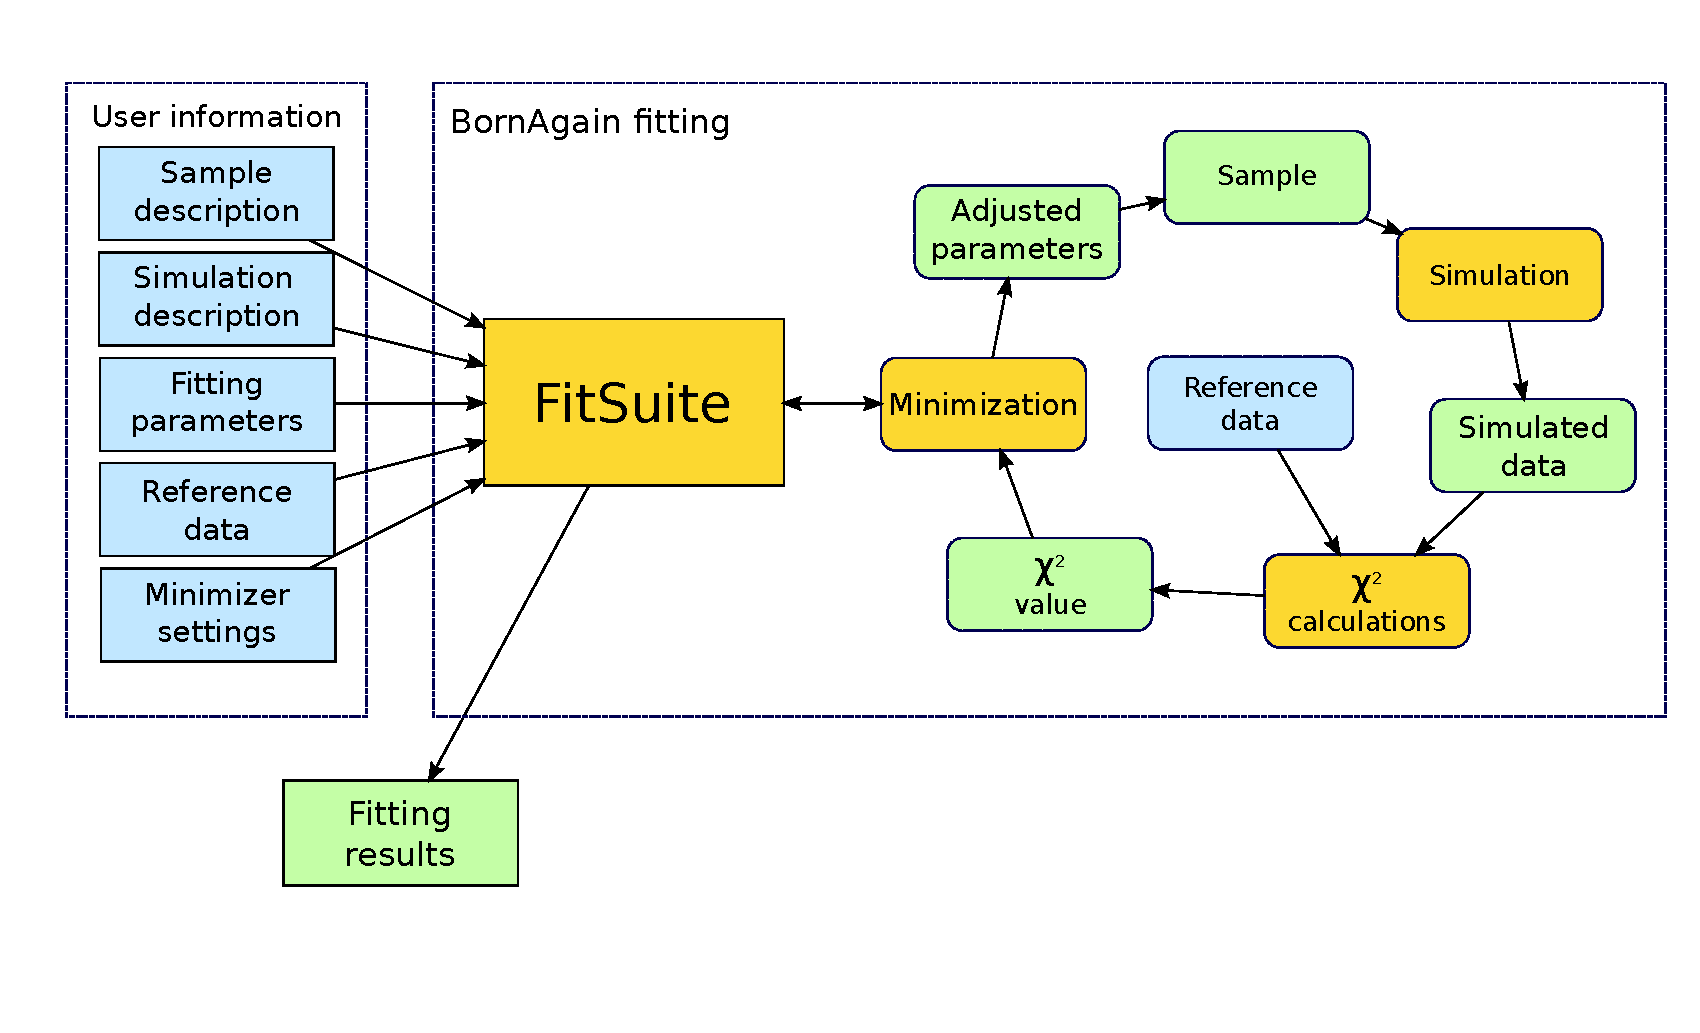
\includegraphics{fig/drawing/minimization_workflow.pdf}}
\caption{
Fitting work flow.
}
\label{fig:minimization_workflow}
\end{figure}

Before running the fitting the user is required to prepare some  data and to
configure the fitting kernel of \BornAgain\ . The required stages are

\begin{itemize}
\item Preparing the sample and the simulation description (multilayer, beam, detector parameters).
\item Choosing the fitting parameters.
\item Loading the reference data.
\item Defining the minimization settings.
\end{itemize}

The class \Code{FitSuite} contains the main functionalities to be used for the fit
and serves as the main interface between the user and the fitting work flow.
The later involves iterations during which

\begin{itemize}
\item The minimizer makes an assumption about the optimal sample parameters.
\item These parameters are propagated to the sample.
\item The simulation is performed for the given state of the sample.
\item The simulated data (intensities) are propagated to the $\chi^2$ module.
\item The later calculates $\chi^2$ using the simulated and reference data.
\item The value of $\chi^2$ is propagated to the minimizer, which makes new assumptions about optimal sample parameters.
\end{itemize}

The iteration process is going on under the control of the selected minimization
algorithm, without any intervention from the
user. It stops
\begin{itemize}
\item when the maximum number of iteration steps has been exceeded,
\item when the function's minimum has been reached within the tolerance window,
\item if the minimizer could not improve the values of the parameters.
\end{itemize}

After the control is returned, fitting results can be retrieved.
They consist in the best $\chi^2$ value found, the corresponding
optimal sample parameters and the intensity map simulated with this set of parameters.

%Details of \Code{FitSuite} class implementation and description of each interface are given in \cref{sec:FitSuiteClass}.
The following parts of this section will detail each of
the main stages necessary to run a fitting procedure.


\subsubsection{Preparing the sample and the simulation description}

This step is similar for any simulation using \BornAgain\ (see \cref{sec:Simulation}). It consists in first characterizing  the geometry of the system: the particles
(shapes, sizes, refractive
indices), the different layers (thickness,
order, refractive index, a possible roughness of the interface), the
interference between the particles and the way they are distributed in
the layers (buried particles or particles sitting on top of a
layer).
Then we specify the parameters of the input beam and of the
output detector.


%===============================================================================
\subsubsection{Choice of parameters to be fitted}
%===============================================================================

In principle, every parameter used in the construction of the sample
can be used as a fitting parameter. For example, the particles'
heights, radii or the layer's roughness or thickness could be selected
using the
parameter pool mechanism.
This mechanism is explained in detail in
\cref{sec:WorkingWithSampleParameters} and it is therefore recommended
to read it before proceeding any further.

The user specifies selected sample parameters as fit parameters using \Code{FitSuite}
and its \Code{addFitParameter} method
\begin{lstlisting}[language=shell, style=commandline]
fit_suite = FitSuite()
fit_suite.addFitParameter(<name>, <initial value>, <step>, <limits>)
\end{lstlisting}
where \Code{<name>} corresponds to the parameter name in the sample's parameter pool.
By using wildcards in the parameter name, a group of sample parameters, corresponding to the given
pattern, can be associated with a single fitting parameter and
fitted simultaneously to get a common optimal value (see \cref{sec:WorkingWithSampleParameters}).

The second parameter \Code <initial value> correspond to the initial value of
the fitting parameter, while the third one
is responsible to the initial iteration steps size.
The last parameter \Code{<AttLimits>} corresponds to
the boundaries imposed on parameter value. It can be
\begin{itemize}
\item \Code{limitless()} by default,
\item \Code{fixed()},
\item \Code{lowerLimited(<min\_value>)},
\item \Code{upperLimited(<max\_value>)},
\item \Code{limited(<min\_value>, <max\_value>)}.
\end{itemize}
where \Code{<min\_value>} and \Code{<max\_value>} are
double values corresponding to the lower and higher boundary, respectively.


%===============================================================================
\subsubsection{Associating reference and simulated data}
%===============================================================================

The minimization procedure deals with a pair of reference data (normally
associated with experimental data) and the theoretical model (presented by the sample and the simulation descriptions).

We assume that the experimental data are a two-dimensional intensity
matrix as function of the output scattering
angles $\alpha_f$ and $\phi_f$ (see \cref{fig:multil3d}).
The user is required to provide the data in the form of an ASCII file
containing an axes
binning description and the intensity data itself.
\vspace*{2mm}

\ImportantPoint{Remark:}{
We recognize the importance of supporting the most common data formats. We are going to provide
this feature in the following releases and welcome users' requests on this subject.
}
\vspace*{1mm}

To associate the simulation and the reference data to the fitting engine, method \newline
\Code{addSimulationAndRealData} has to be used as shown
\begin{lstlisting}[language=python, style=eclipseboxed,numbers=none]
fit_suite = FitSuite()
fit_suite.addSimulationAndRealData(<simulation>, <reference>, <chi2_module>)
\end{lstlisting}

Here \Code{<simulation>} corresponds to a \BornAgain\ simulation object
with the  sample, beam and detector fully defined, \Code{<reference>}
corresponds to the experimental data object obtained from the ASCII file and \Code{<chi2\_module>} is an optional parameter for advanced
control of $\chi^2$ calculations.

It is possible to call this given method more than once to submit more than one pair of
\Code{<simulation>, <reference>} to the fitting procedure.
In this way, simultaneous fits of
some combined data sets are performed.

By using the third parameter, \Code{<chi2\_module>}, different normalizations and weights
can be applied to give user full control of the way $\chi^2$ is calculated.
This feature will be explained in \cref{sec:FittingAdvanced}.


%===============================================================================
\subsection{Minimizer settings}
%===============================================================================

\BornAgain\ contains a variety of minimization engines from \Code{ROOT} and \Code{GSL}
libraries. They are listed in Table~\ref{table:fit_minimizers}.
By default \Code{Minuit2} minimizer with default settings will be used and no additional
configuration needs to be done.
The remainder of this section explains some of the expert settings, which can be applied to get better
fit results.

The default minimization algorithm can be changed using
\Code{MinimizerFactory} as shown below
\begin{lstlisting}[language=python, style=eclipseboxed,numbers=none]
fit_suite = FitSuite()
minimizer = MinimizerFactory.createMinimizer("<Minimizer name>","<algorithm>")
fit_suite.setMinimizer(minimizer)
\end{lstlisting}

where \Code{<Minimizer name>} and \Code{<algorithm>} can be chosen from the first and
second column of Table~\ref{table:fit_minimizers} respectively.
The list of minimization algorithms implemented in \BornAgain\
can also be obtained using \Code{MinimizerFactory.printCatalogue()} command.


\begin{table}[h]
  \small
\centering
\begin{tabular}{@{}lll@{}}
\hline
\hline
\textbf{Minimizer name} & \textbf{Algorithm} & \textbf{Description}\\
\hline
\Code{Minuit2} \cite{MinuitURL} & \Code{Migrad} & According to
\cite{mntutorial} best minimizer for nearly all functions,\\
 & & variable-metric method with inexact line search, \\
 & & a stable metric updating scheme,\\
 & &  and checks for positive-definiteness.\\
\hline
                                       & \Code{Simplex} & simplex method of
                                       Nelder and Mead\\
 & & usually slower than \Code{Migrad}, \\
 &  & rather robust with respect to gross fluctuations in the\\ & &  function
 value, gives no reliable information about \\ & &  parameter errors, \\
\hline
                                       & \Code{Combined} & minimization with
                                       \Code{Migrad} \\
                                       & & but switches to Simplex if
                                       Migrad fails to converge.\\
\hline
                                       & \Code{Scan} &  not intended to
                                       minimize, just scans the
                                       function,\\
                                       & &  one parameter at a
                                       time, retains the best value
                                       after\\ &  & each scan\\
\hline
                                       & \Code{Fumili} & optimized
                                       method for least square and log
                                       likelihood\\ & &  minimizations \\
\hline
\Code{GSLMultiMin} \cite{GSLMultiMinURL} & \Code{ConjugateFR} & Fletcher-Reeves conjugate gradient
  algorithm,\\
\hline
& \Code{ConjugatePR} & Polak-Ribiere conjugate gradient algorithm,\\
\hline
& \Code{BFGS} & Broyden-Fletcher-Goldfarb-Shanno algorithm,\\
\hline
& \Code{BFGS2} & improved version of BFGS,\\
\hline
& \Code{SteepestDescent} & follows the downhill gradient of the function at each step\\
\hline
\Code{GSLLMA} \cite{GSLMultiFitURL} & & Levenberg-Marquardt
Algorithm\\
\hline
\Code{GSLSimAn} \cite{GSLSimAnURL}& & Simulated Annealing Algorithm\\
\hline
\hline
\end{tabular}
\caption{List of minimizers implemented in \BornAgain. }
\label{table:fit_minimizers}
\index{Minimizers}
\end{table}

There are several options common to every minimization algorithm, which can be changed
before starting the minimization. They are handled by \Code{MinimizerOptions} class:
\begin{lstlisting}[language=python, style=eclipseboxed, numbers = none]
fit_suite.getMinimizer().getOptions().setMaxFunctionCalls(10)
\end{lstlisting}
In the above code snippet, a number of ``maximum function calls'',
namely the maximum number of times the minimizer is allowed to call the simulation, is limited to 10. %The minimizer will take that number into consideration and will try to limit number of iterations by that value.

There are also expert-level options common for all minimizers as well
as a number of options to tune individual minimization algorithms.
They will be explained in \cref{sec:FittingAdvanced}.


%===============================================================================
\subsection{Running the fitting ant retrieving the results}
%===============================================================================

After the initial configuration of \Code{FitSuite} has been performed, the fitting
can be started using the command
\begin{lstlisting}[language=python, style=eclipseboxed, numbers = none]
fit_suite.runFit()
\end{lstlisting}

Depending on the complexity of the sample and the number of free sample parameters the fitting
process can take from tens to thousands of iterations. The results of the fit can
be printed on the screen using the command
\begin{lstlisting}[language=python, style=eclipseboxed, numbers = none]
fit_suite.printResults()
\end{lstlisting}
\cref{sec:FittingExamples} gives more details about how to access the fitting results.


%===============================================================================
\subsection{Basic Python fitting example} \label{sec:FittingExamples}
%===============================================================================

In this section we are going to go through a complete example of
fitting using \BornAgain. Each  step will be associated with a
detailed piece of code written in \Python.
The complete listing of
the script is given in Appendix (see Listing~\ref{PythonFittingExampleScript}).
The script can also be found at
\begin{lstlisting}[language=shell, style=commandline]
./Examples/python/fitting/ex002_FitCylindersAndPrisms/FitCylindersAndPrisms.py
\end{lstlisting}

\noindent
This example uses the same sample geometry as in \cref{sec:Example1Python}.
Cylindrical and
prismatic particles in equal proportion are deposited on a substrate layer, with no interference
between the particles. We consider the following parameters to be unkown
\begin{itemize}
\item the radius of cylinders,
\item the height of cylinders,
\item the length of the prisms' triangular basis,
\item the height of prisms.
\end{itemize}

Our reference data are a ``noisy'' two-dimensional intensity
map obtained from the simulation of the same geometry with a fixed
value of $5\,{\rm nm}$ for the height and radius of cylinders and for the
height of prisms which have a 10-nanometer-long side length.
Then we run our fitting using default minimizer settings
starting with a cylinder's height
of $4\,{\rm nm}$, a cylinder's radius of $6\,{\rm nm}$,
a prism's half side of $6\,{\rm nm}$ and a height equal to $4\,{\rm nm}$.
As a result, the fitting procedure is able to find the correct value of $5\,{\rm nm}$
for all four parameters.


%-------------------------------------------------------------------------------
\subsubsection*{Importing Python libraries}
%-------------------------------------------------------------------------------

\begin{lstlisting}[language=python, style=eclipseboxed]
from libBornAgainCore import *
from libBornAgainFit import *
\end{lstlisting}
We start from importing two \BornAgain\ libraries required to create
the sample description
and to run the fitting.

%-------------------------------------------------------------------------------
\subsubsection*{Building the sample}
%-------------------------------------------------------------------------------

\begin{lstlisting}[language=python, style=eclipseboxed, firstnumber=5]
def get_sample(): @\label{script2::get_sample}@
    """
    Build the sample representing cylinders and pyramids on top of substrate without interference.
    """
    # defining materials
    m_air = HomogeneousMaterial("Air", 0.0, 0.0)
    m_substrate = HomogeneousMaterial("Substrate", 6e-6, 2e-8)
    m_particle = HomogeneousMaterial("Particle", 6e-4, 2e-8)

    # collection of particles
    cylinder_ff = FormFactorCylinder(1.0*nanometer, 1.0*nanometer)
    cylinder = Particle(m_particle, cylinder_ff)
    prism_ff = FormFactorPrism3(2.0*nanometer, 1.0*nanometer)
    prism = Particle(m_particle, prism_ff)
    particle_layout = ParticleLayout()
    particle_layout.addParticle(cylinder, 0.5)
    particle_layout.addParticle(prism, 0.5)
    interference = InterferenceFunctionNone()
    particle_layout.addInterferenceFunction(interference)

    # air layer with particles and substrate form multi layer
    air_layer = Layer(m_air)
    air_layer.addLayout(particle_layout)
    substrate_layer = Layer(m_substrate)
    multi_layer = MultiLayer()
    multi_layer.addLayer(air_layer)
    multi_layer.addLayer(substrate_layer)
    return multi_layer
\end{lstlisting}
The function starting at line~\ref{script2::get_sample} creates a multilayered sample
with cylinders and prisms using arbitrary $1\,{\rm nm}$ value for all size's of particles.
The details about the generation of this multilayered sample are given in \cref{sec:Example1Python}.

%-------------------------------------------------------------------------------
\subsubsection*{Creating the simulation}
%-------------------------------------------------------------------------------
\begin{lstlisting}[language=python, style=eclipseboxed, firstnumber=35]
def get_simulation(): @\label{script2::get_simulation}@
    """
    Create GISAXS simulation with beam and detector defined
    """
    simulation = Simulation()
    simulation.setDetectorParameters(100, -1.0*degree, 1.0*degree, 100, 0.0*degree, 2.0*degree)
    simulation.setBeamParameters(1.0*angstrom, 0.2*degree, 0.0*degree)
    return simulation
\end{lstlisting}
The function starting at line~\ref{script2::get_simulation} creates
the simulation object with the definition of the beam and detector parameters.

%-------------------------------------------------------------------------------
\subsubsection*{Preparing the fitting pair}
%-------------------------------------------------------------------------------
\begin{lstlisting}[language=python, style=eclipseboxed, firstnumber=45]
def run_fitting(): @\label{script2::run_fitting}@
    """
    run fitting
    """
    sample = get_sample() @\label{script2::setup_simulation1}@
    simulation = get_simulation()
    simulation.setSample(sample) @\label{script2::setup_simulation2}@

    real_data = IntensityDataIOFactory.readIntensityData('refdata_fitcylinderprisms.int.gz') @\label{script2::real_data}@
\end{lstlisting}
Lines
~\ref{script2::setup_simulation1}-~\ref{script2::setup_simulation2}
generate the
sample and simulation description and assign the sample to the simulation.
Our reference data are contained in the file \Code{'refdata\_fitcylinderprisms.int.gz'}.
 This reference had been generated by adding noise
on the scattered intensity from a numerical sample with a fixed length of 5~nm for the four fitting
parameters (\idest the dimensions of the cylinders and prisms).
Line ~\ref{script2::real_data} creates the real data object by loading
the ASCII data from the input file.

%-------------------------------------------------------------------------------
\subsubsection*{Setting up \rm\bf{FitSuite}}
%-------------------------------------------------------------------------------
\begin{lstlisting}[language=python, style=eclipseboxed, firstnumber=55]
    fit_suite = FitSuite() @\label{script2::fitsuite1}@
    fit_suite.addSimulationAndRealData(simulation, real_data) @\label{script2::fitsuite2}@
    fit_suite.initPrint(10) @\label{script2::fitsuite3}@
\end{lstlisting}
Line ~\ref{script2::fitsuite1} creates a \Code{FitSuite} object which provides
the main interface to the minimization kernel of \BornAgain\ .
Line ~\ref{script2::fitsuite2} submits simulation description and real data pair to the
subsequent fitting. Line ~\ref{script2::fitsuite3} sets up \Code{FitSuite} to print on
the screen the information about fit progress once per 10 iterations.
\begin{lstlisting}[language=python, style=eclipseboxed, firstnumber=60]
    fit_suite.addFitParameter("*FormFactorCylinder/height", 4.*nanometer, 0.01*nanometer, AttLimits.lowerLimited(0.01)) @\label{script2::fitpars1}@
    fit_suite.addFitParameter("*FormFactorCylinder/radius", 6.*nanometer, 0.01*nanometer, AttLimits.lowerLimited(0.01))
    fit_suite.addFitParameter("*FormFactorPrism3/height", 4.*nanometer, 0.01*nanometer, AttLimits.lowerLimited(0.01))
    fit_suite.addFitParameter("*FormFactorPrism3/length", 12.*nanometer, 0.02*nanometer, AttLimits.lowerLimited(0.01)) @\label{script2::fitpars2}@
\end{lstlisting}
Lines ~\ref{script2::fitpars1}--~\ref{script2::fitpars2} enter the
list of fitting parameters. Here we use the cylinders' height and
radius and the prisms' height and side length.
The cylinder's length and prism half side are initially equal to $4\,{\rm nm}$,
whereas the cylinder's radius and the prism half side length are equal to $6\,{\rm nm}$ before the minimization. The
iteration step is equal to $0.01\,{\rm nm}$ and only the lower
boundary is imposed to be equal to $0.01\,{\rm nm}$.

%-------------------------------------------------------------------------------
\subsubsection*{Running the fit and accessing results}
%-------------------------------------------------------------------------------
\begin{lstlisting}[language=python, style=eclipseboxed, firstnumber=66]
    fit_suite.runFit() @\label{script2::fitresults1}@

    print "Fitting completed."
    fit_suite.printResults()@\label{script2::fitresults2}@
    print "chi2:", fit_suite.getMinimizer().getMinValue()
    fitpars = fit_suite.getFitParameters()
    for i in range(0, fitpars.size()):
        print fitpars[i].getName(), fitpars[i].getValue(), fitpars[i].getError() @\label{script2::fitresults3}@
\end{lstlisting}
Line ~\ref{script2::fitresults1} shows the command to start the fitting process.
During the fitting the progress will be displayed on the screen.
Lines ~\ref{script2::fitresults2}--~\ref{script2::fitresults3} shows different ways of
accessing the fit results.


More details about fitting, access to its results and visualization of
the fit progress using matplotlib libraries can be learned from the
following detailed example
\begin{lstlisting}[language=shell, style=commandline]
./Examples/python/fitting/ex002_FitCylindersAndPrisms/FitCylindersAndPrisms_detailed.py
\end{lstlisting}


%===============================================================================
\subsection{Advanced fitting} \label{sec:FittingAdvanced}
%===============================================================================

\subsubsection{Affecting chi-square calculations}
\MissingSection
\subsubsection{Simultaneous fits of several data sets}
\MissingSection
\subsubsection{Using fitting strategies}
\MissingSection
\subsubsection{Masking the real data}
\MissingSection
\subsubsection{Tuning fitting algorithms}
\MissingSection
\subsubsection{Fitting with correlated sample parameters}
\MissingSection


%===============================================================================
\subsection {How to get the right answer from fitting}
  \label{sec:FittingRightAnswers}
%===============================================================================

%As it has already been mentioned in \cref{sec:FittingGentleIntroducion},
One of the main difficulties in fitting the data with the model
is the presence of multiple
local minima in the objective function. Many problems can cause the
fit to fail, for example:
\begin{itemize}
\item an unreliable physical model,
\item an unappropriate choice of objective function
\item multiple local minima,
\item an unphysical behavior of the objective function, unphysical regions
  in the parameters space,
\item an unreliable parameter error calculation in the presence of
  limits on the parameter value,
\item an exponential behavior of the objective function and the
  corresponding numerical inaccuracies, excessive numerical roundoff
  in the calculation of its value and derivatives,
\item large correlations between parameters,
\item very different scales of parameters involved in the calculation,
\item not positive definite error matrix even at minimum.
\end{itemize}


The given list, of course, is not only related to \BornAgain\
fitting. It remains applicable to any fitting program and any kind of theoretical model.
%To address all these difficulties some amount of manual tuning might be necessary.
 Below we give some recommendations which might help the user to achieve reliable fit results.

\subsection*{General recommendations}
\begin{itemize}
\item initially choose  a small number of free fitting parameters,
\item eliminate redundant parameters,
\item provide a good initial guess for the fit parameters,
\item start from the default minimizer settings and perform some fine tuning after some experience has been acquired,
\item repeat the fit using different starting values for the parameters or their limits,
\item repeat the fit, fixing and varying different groups of parameters,
%\item use \Code{Minuit2} minimizer with \Code{Migrad} algorithm
%  (default) to get the most reliable parameter error estimation,
%\item try \Code{GSLMultiFit} minimizer or \Code{Minuit2} minimizer with \Code{Fumili} %algorithm to get fewer iterations.
\end{itemize}

\Work{... to be continued ...}

%\subsection*{Interpretation of errors.}

\index{Fitting|)}

%%%%%%%%%%%%%%%%%%%%%%%%%%%%%%%%%%%%%%%%%%%%%%%%%%%%%%%%%%%%%%%%%%%%%%%%%%%%%%%%
\section{User API} \label{UserAPI}
%%%%%%%%%%%%%%%%%%%%%%%%%%%%%%%%%%%%%%%%%%%%%%%%%%%%%%%%%%%%%%%%%%%%%%%%%%%%%%%%

%===============================================================================
\subsection{IntensityData}
%===============================================================================

The \Code{IntensityData} object stores the
simulated or real intensity data together with the axes definition of the detector in BornAgain's internal format.
During the simulation setup
it is created automatically when the user specifies the detector characteristics and is filled with the simulated intensities after the simulation is completed.

\begin{lstlisting}[language=python, style=eclipseboxed]
simulation = Simulation()
simulation.setDetectorParameters(10, -5.0*degree, 5.0*degree, 5, 0.0*degree, 1.0*degree)
...
simulation.runSimulation()
intensity = simulation.getIntensityData() @\label{py:UserApi:intensity}@
\end{lstlisting}

The \Code{IntensityData} object retrieved in line~\ref{py:UserApi:intensity} corresponds to
the two dimensional detector pixel array as shown in \cref{fig:UserApi:IntensityData}.

\begin{figure}[ht]
  \centering
    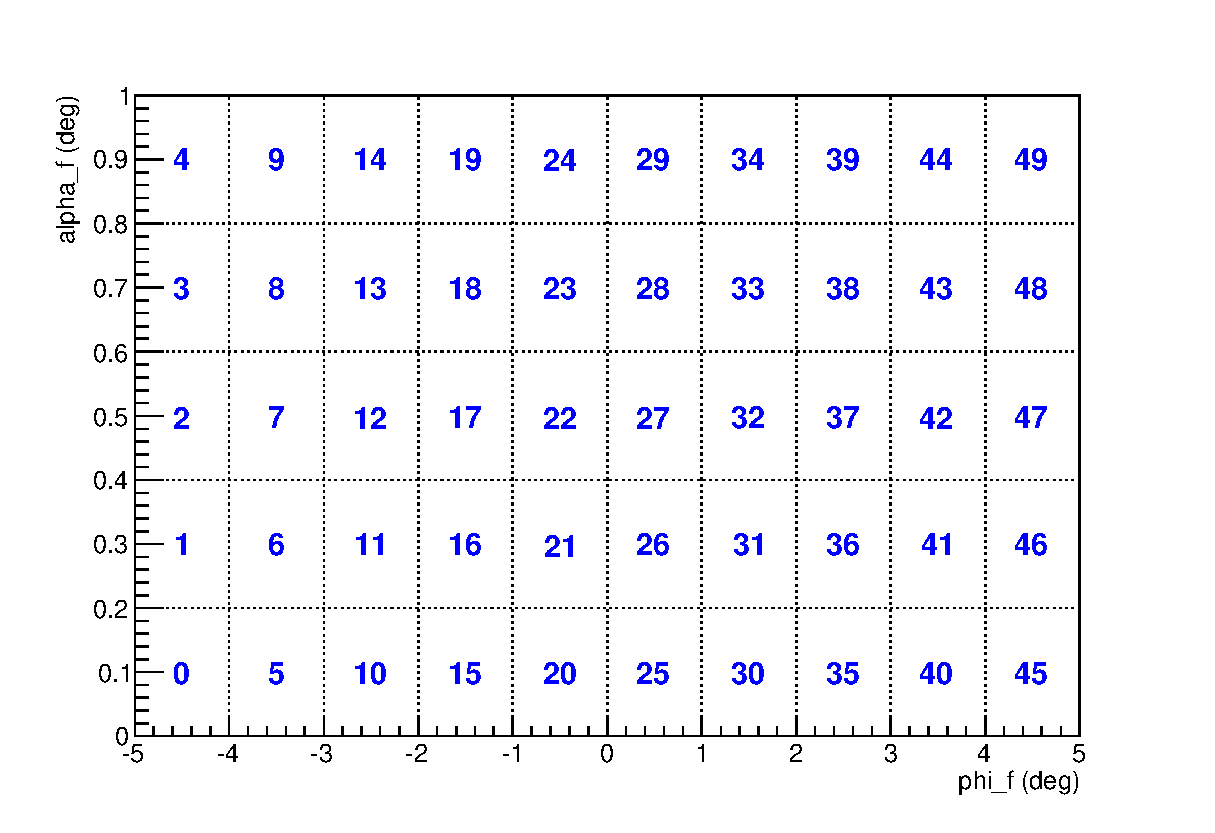
\includegraphics[clip=, width=120mm]{fig/drawing/UserAPI_IntensityDataLayout.eps}
  \caption{The axes layout of IntensityData object.}
  \label{fig:UserApi:IntensityData}
\end{figure}

The x-axis and y-axis of the figure correspond to the $\phi_f$ and $\alpha_f$ axes of the detector.
The x-axis is divided into 10 bins,
with low edge of the first bin set to $-5.0\,{\rm deg}$ and upper edge of the last bin set to $+5.0\,{\rm deg}$.
The y-axis is divided into 5 bins,
with low edge of the first bin set to $0.0\,{\rm deg}$ and upper edge of the last bin set to $1.0\,{\rm deg}$.
There are 50 bins in total (they are marked on the plot with indexes from 0 to 49), each bin will contain one intensity value.

During a standard simulation (i.e. no Monte-Carlo integration involved) intensities are calculated for $\phi_f, \alpha_f$ values corresponding to the bin centers, e.g. the intensity stored in bin\#42 will correspond to $\phi_f=3.5\,{\rm deg}, \alpha_f=0.5\,{\rm deg}$.
\vspace*{2mm}


\MakeRemark{}{
The \Code{IntensityData} object is not intended for direct usage from Python API. The idea is
that the API provides the user with the possibility to export the data from BornAgain internal format to the format of his choice as well as import user's data into BornAgain.
For the moment this functionality is limited to a few options explained below.
We encourage users feedback to implement the support of most requested formats.
}\\



\subsubsection{Import/export of intensity data}
For the moment we provide following options:
\begin{itemize}
\item Import/export of \Code{IntensityData} object from/to \Code{numpy} array.
\item Import/export of \Code{IntensityData} object from/to text file.

\end{itemize}

\paragraph{Export to numpy array}

To export intensity data into  \Code{numpy} array the method \Code{getArray()} should be used
on \Code{IntensityData} object as shown in line \ref{py:UserApi:getArray} of
following code snippet.

\begin{lstlisting}[language=python, style=eclipseboxed]
intensity = simulation.getIntensityData()
array = intensity.getArray() @\label{py:UserApi:getArray}@
...
pylab.imshow(numpy.rot90(array, 1)) @\label{py:UserApi:imshow}@
pylab.show()
\end{lstlisting}

For the detector settings defined in the previous paragraph the dimensions of the resulting array will be (10,5). By using \Code{numpy} indexes the user can get access to the intensity values, e.g.
\Code{array[0][0]} corresponds to the intensity in bin\#0 of \cref{fig:UserApi:IntensityData},
\Code{array[0][4]} to bin\#4,
\Code{array[1][0]} to bin\#5,
\Code{array[8][2]} to bin\#42,
\Code{array[9][4]} to bin\#49.


To plot this resulting numpy array with \Code{matplotlib} it has to be rotated counter-clockwise
to match \Code{matplotlib} conventions as shown in line~\ref{py:UserApi:imshow}.


%\subsubsection{Direct access to the data}
%User can access to the

%\begin{lstlisting}[language=python, style=eclipseboxed]
%for i in range(0, intensity.getAllocatedSize()):
%    print intensity[i]
%\end{lstlisting}


\subsubsection{Importing from numpy array}

To use fitting the user has to load experimental data into BornAgain fitting kernel.
To read experimental data the user has to create
IntensityData object, fill it with the experimental  intensity values and pass
this object to the fitting kernel.

First, the user creates empty \Code{IntensityData} as shown
in line~\ref{py:UserApi:IntensityData} of the following code snippet.
\begin{lstlisting}[language=python, style=eclipseboxed]
data = IntensityData() @\label{py:UserApi:IntensityData}@
data.addAxis(FixedBinAxis("phi_f", 10, -5.0*degree, 5.0*degree)) @\label{py:UserApi:phi_f}@
data.addAxis(FixedBinAxis("alpha_f", 5, 0.0*degree, 1.0*degree)) @\label{py:UserApi:alpha_f}@
...
array = numpy.zeros((10, 5)) # fill array with experimental intensities @\label{py:UserApi:create_array}@
...
data.setRawDataVector(array.flatten().tolist()) @\label{py:UserApi:set_raw}@

fitSuite = FitSuite() @\label{py:UserApi:fit_suite}@
fitSuite.addSimulationAndRealData(simulation, data) @\label{py:UserApi:add_real_data}@
\end{lstlisting}

In lines~\ref{py:UserApi:phi_f}, \ref{py:UserApi:alpha_f} two axes with fixed bin sizes
are defined to represent the detector layout as shown in \cref{fig:UserApi:IntensityData}.
The constructor of \Code{FixedBinAxis} object has the following signature

\begin{lstlisting}[language=python, style=eclipse,numbers=none]
FixedBinAxis(title, nbins, min_angle, max_angle)
\end{lstlisting}

The created \Code{IntensityData} object has to be filled with experimental intensities
using \Code{numpy} array prepared by the user (lines ~\ref{py:UserApi:create_array}-~\ref{py:UserApi:set_raw}). In lines \ref{py:UserApi:fit_suite},\ref{py:UserApi:add_real_data} the fitting kernel is created and initialized with \Code{Simulation} object and
\Code{IntensityData} object representing the experimental data.


\subsubsection{Saving intensity data to text file.}

The special class \Code{IntensityDataIOFactory} is intended for saving the intensity data
in different datafile formats. For the moment, it only supports saving the data in specific BornAgain's text files (the file extention \Code{*.int}).

\begin{lstlisting}[language=python, style=eclipseboxed]
intensity = simulation.getIntensityData()
IntensityDataIOFactory.writeIntensityData(intensity, 'file_name.int')
\end{lstlisting}

\subsubsection{Reading intensity data from a text file.}
The same class is also intended for reading intensity data
from files with different formats. For the moment, it only supports reading the data from text files of special BornAgain's format (the file extention \Code{*.int}).

\begin{lstlisting}[language=python, style=eclipseboxed]
intensity = IntensityDataIOFactory.readIntensityData('file_name.int')
\end{lstlisting}

%%%%%%%%%%%%%%%%%%%%%%%%%%%%%%%%%%%%%%%%%%%%%%%%%%%%%%%%%%%%%%%%%%%%%%%%%%%%%%%%%
%%
%%   BornAgain:  simulate and fit scattering at grazing incidence
%%
%%   homepage:   http://www.bornagainproject.org
%%
%%   copyright:  Forschungszentrum Jülich GmbH 2015
%%               Software licence does not cover this documentation
%%               For documentation licence, contact the authors
%%   
%%   authors:    Scientific Computing Group at MLZ Garching
%%               C. Durniak, M. Ganeva, G. Pospelov, W. Van Herck, J. Wuttke
%%
%%%%%%%%%%%%%%%%%%%%%%%%%%%%%%%%%%%%%%%%%%%%%%%%%%%%%%%%%%%%%%%%%%%%%%%%%%%%%%%%


\newpage
\chapter{Fitting} \SecLabel{Fitting}

In addition to the simulation of grazing incidence
X-ray and neutron scattering by
multilayered samples, \BornAgain\ also offers the option to
fit the numerical model to reference data by modifying a selection of
sample parameters from the numerical model.  This aspect
of the software is discussed in the current chapter.

%\SecRef{FittingGentleIntroducion} gives a short introduction to the
%basic concepts of data fitting. Users familiar with fitting can
%directly proceed to \SecRef{FittingImplementation}, which details the
%implementation of fittings in 
%\BornAgain\ . 
\SecRef{FittingImplementation} details the
implementation of fittings in \BornAgain\ . 
\Python\ fitting examples with detailed
explanations of every fitting step are given in \SecRef{FittingExamples}. Advanced fitting techniques, including fine tuning of minimization
algorithms, simultaneous fits of different data sets, parameters
correlation, are covered in
\SecRef{FittingAdvanced}. \SecRef{FittingRightAnswers} contains some practical advice, which might
help the user to get right answers from \BornAgain\ fitting.

%%%%%%%%%%%%%%%%%%%%%%%%%%%%%%%%%%%%%%%%%%%%%%%%%%%%%%%%%%%%%%%%%%%%%%%%%%%%%%%%
%
%%%%%%%%%%%%%%%%%%%%%%%%%%%%%%%%%%%%%%%%%%%%%%%%%%%%%%%%%%%%%%%%%%%%%%%%%%%%%%%
\section{Gentle introduction to the data fitting.} \SecLabel{FittingGentleIntroducion}

The aim of this section is to briefly introduce the basic concept of
data fitting, its key terminology and difficulties which might arise in scattering data fit.
Users wanting to find out more about minimization (also called
maximization or optimization methods depending on the formulations and objectives) 
or looking for more rigorous discussion than provided in this manual
are referred to \cite{Antoniou2007, mntutorial}

\subsection{Toy scattering experiment.}

Fig.~\ref{fig:toyfit_data},left shows scattering intensity map in arbitrary units  
as a function of (x,y) of the detector ``measured'' in toy scattering experiment.

\begin{figure}[!p]
  \centering
    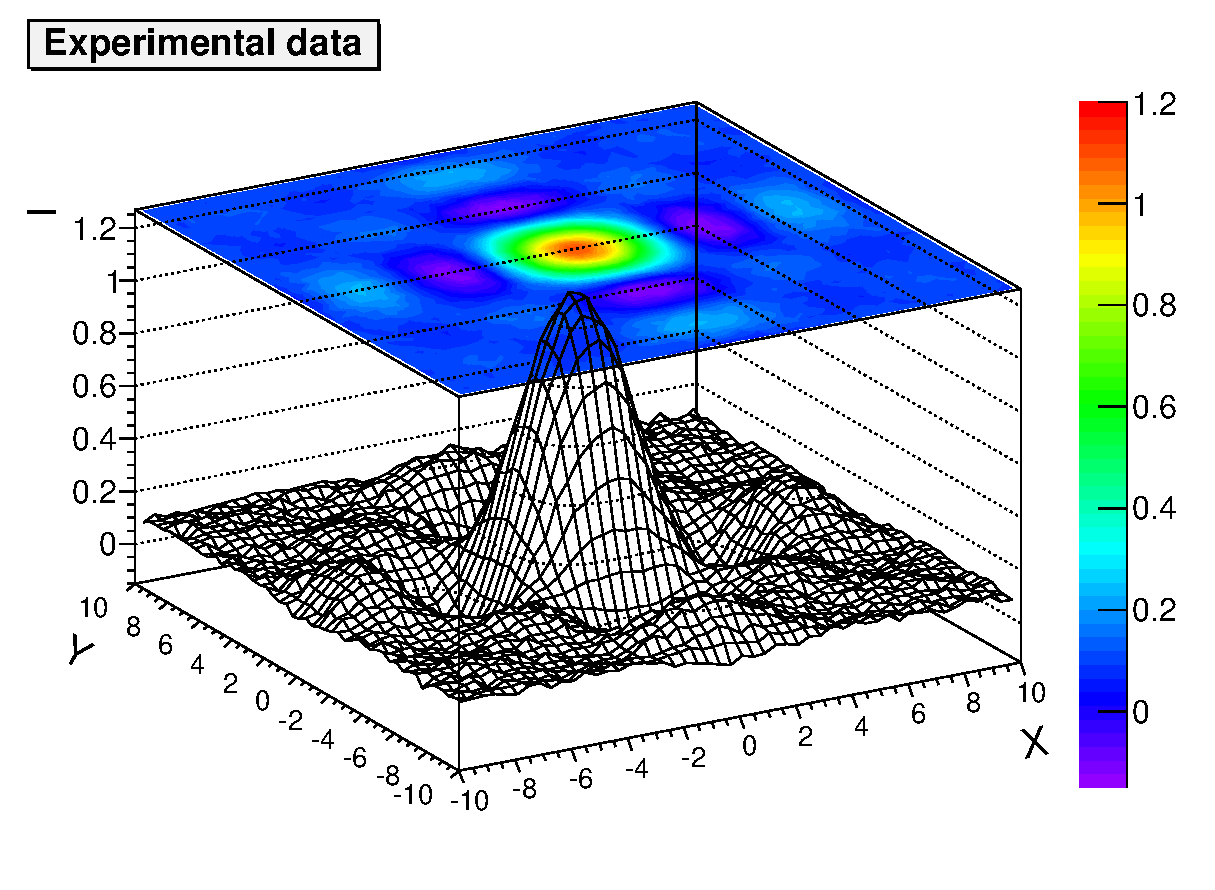
\includegraphics[width=0.49\textwidth]{Figures/toyfit_expdata.eps}
    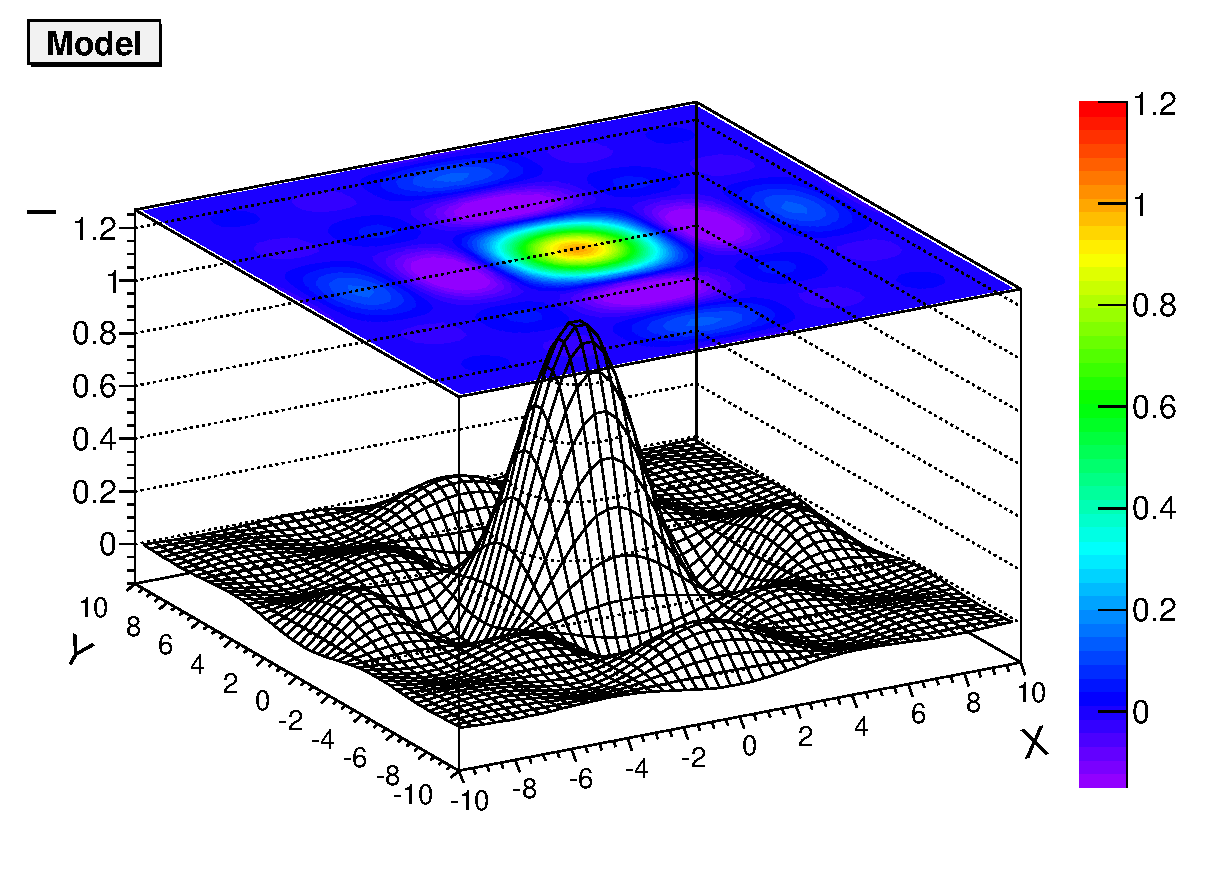
\includegraphics[width=0.49\textwidth]{Figures/toyfit_simdata.eps}
  \caption{Intensity as a function of (x,y) detector coordinates  obtained from 
  toy experiment (left) and from the toy simulation (right).   }
  \label{fig:toyfit_data}
  \vspace*{4mm}
    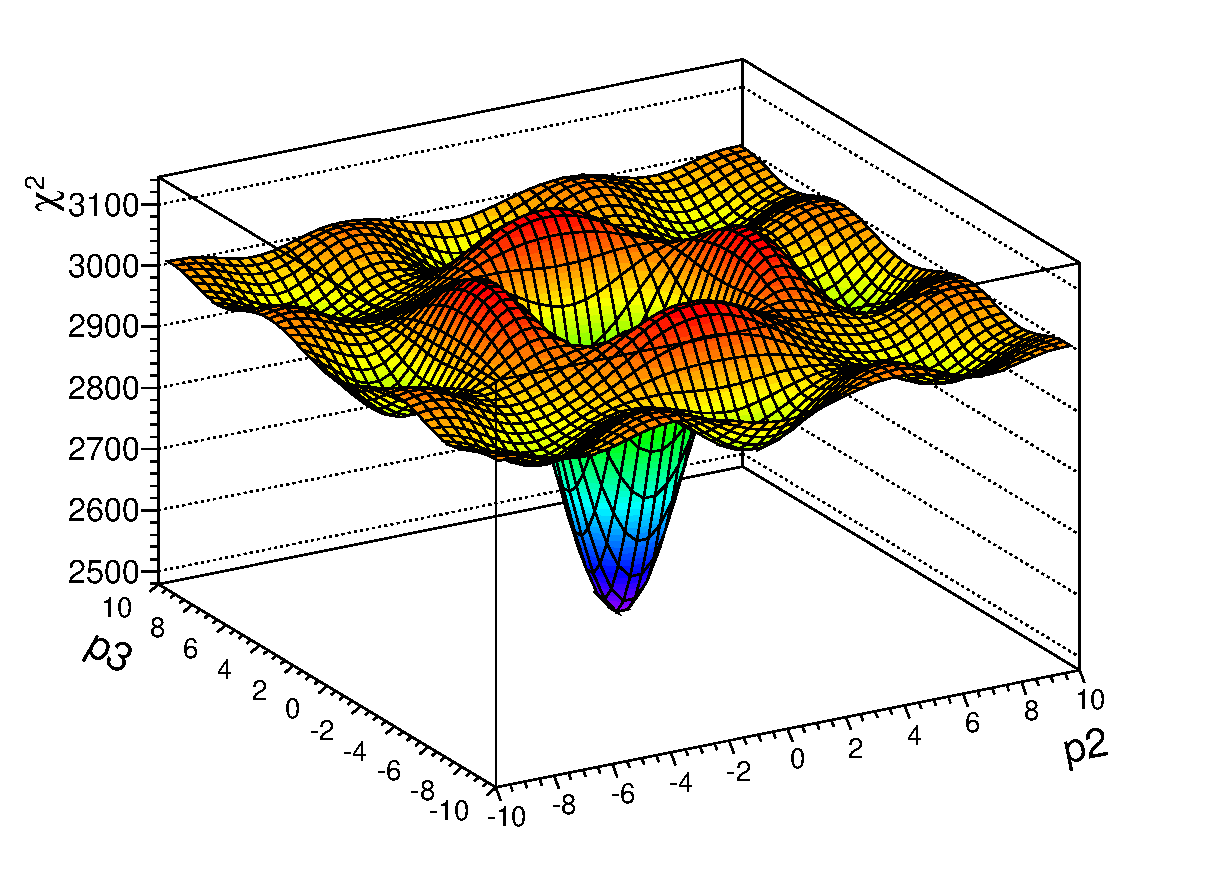
\includegraphics[width=0.49\textwidth]{Figures/toyfit_chi2_p23.eps}
    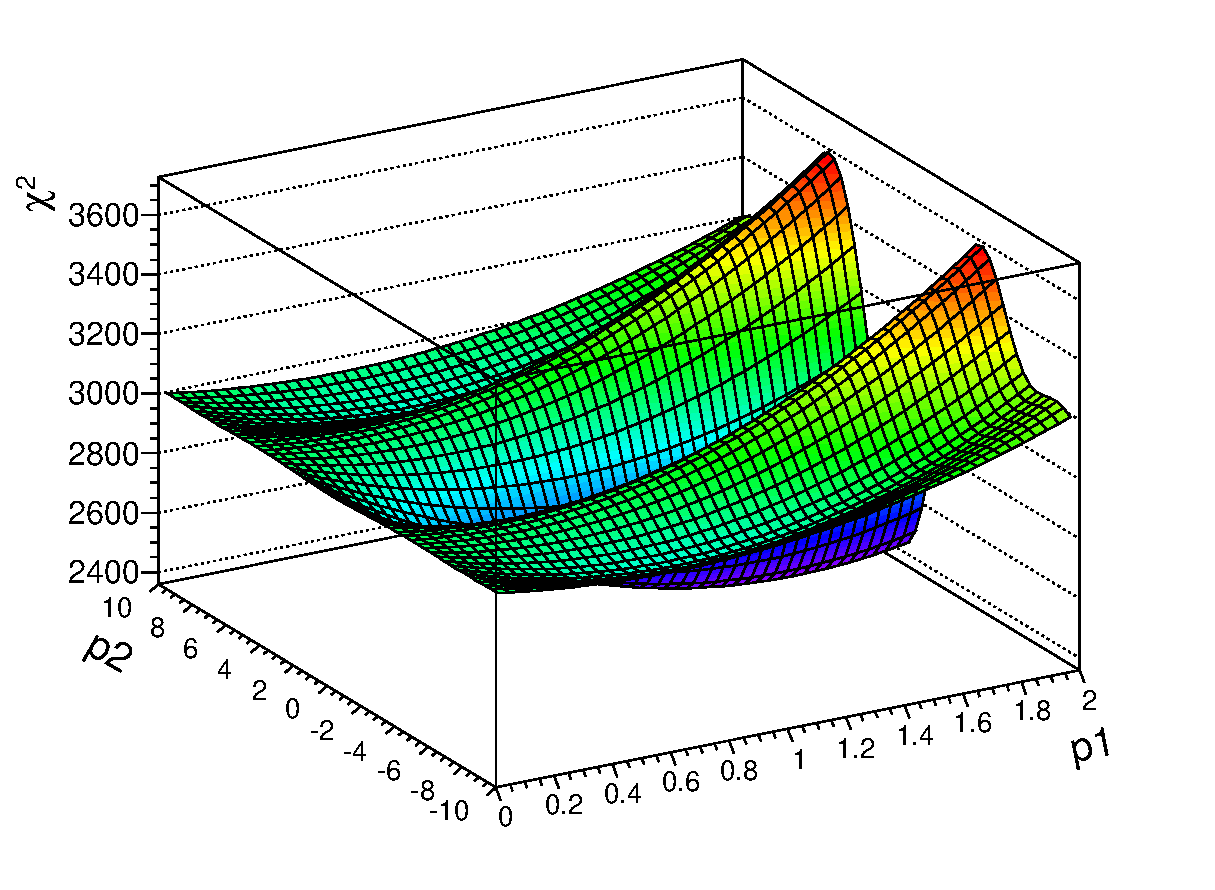
\includegraphics[width=0.49\textwidth]{Figures/toyfit_chi2_p12.eps}
  \caption{$\chi^{2}$ value calculated between experimental and simulated data
  as a function of $p_2,p_3$ parameters (left) or $p_1,p_2$ 
  parameters (right) used in the model.   }
  \label{fig:toyfit_chi2}
\end{figure}


Scattering picture presented reminds some of GISAS patterns, nevertheless it is
generated using simple function
$$I(x,y) = G(0.1,~0.01) + \frac{sin(x)}{x} \cdot \frac{sin(y)}{y}$$
Here $G(0.1, 0.01)$ is a random variable distributed according to the Gaussian distribution
with mean 0.1 and $\sigma=0.01$.
Constant $0.1$ symbolize our experimental background and constant $0.01$ is referred
to the detector noise. The rest of the formula represents our signal.

Lets define our model, namely specific mathematical function, to which we will fit our toy experimental data. By making an educated guess we assume that scattering intensity observed
in the experiment should be described with the help of $sinc$ function as follows
$$ f(x,y) = p_0 + p_1 \cdot  sinc(x - p_2) \cdot sinc(y - p_3) $$
The model has four parameters: $p_0$ describing background, $p_{1}$ describing signal strength
and $p_2,p_3$ responsible for the peak position.
Fig.~\ref{fig:toyfit_data},right shows the intensity as a function (x,y) calculated according
our model using fixed parameter set $p_0=0,p_1=1,p_2=0,p_3=0$. 

Two distributions look pretty much the same, however to find exact values of parameters which describe experimental data in the best way, one have to
\begin{itemize}
\item elaborate criteria for the difference between an actual data and its model
\item employ minimization procedure which will minimize that difference
\end{itemize}


\subsection{Objectives}

The goal is to obtain the best fit of an observed distribution
to a prediction by modifying a set of parameters from the
prediction. This problem can be one or multi-dimensional and also linear or
nonlinear. The quantity to minimize is often referred to as the
\textit{objective function}, whose expression depends on the
particular method, like the maximum likelihood, the $\chi^2$
minimization or the expected prediction error function. 

\begin{comment}
\subsubsection*{Maximum of likelihood.}
This is a popular method for parameters' estimations because the maximum likelihood estimators are approximately
unbiased and efficient for large data samples, under quite general
conditions.
We assume a sample  $\mathbf{x}=\{x_{1},x_{2},...,x_{n}\}$ of n independent and identically distributed
observations coming from probability density function $f(\mathbf{x}; \mathbf{p})$.
We assume $f(\mathbf{x}; \mathbf{p})$
to be known except for the parameters $\mathbf{p}=\{p_1,p_2,...,p_3\}$
The method of maximum likelihood takes the estimators to be
those values of $\mathbf{p}$ that maximize the likelihood function $\mathcal{L}$ as
$\mathcal{L}(\mathbf{\alpha})=\prod_{i=1}^N f(x_i;\mathbf{p})$.
Since it is easier to deal with a sum, we usually minimize
$-\text{ln}(\mathcal{L})$.
\end{comment}


\subsubsection*{$\chi^2$ or least squares minimization}
A dataset consist of $n$ data pairs $(\mathbf{x_{i}}, a_{i}), i=1,N$ where 
$\mathbf{x_{i}}$ is an independent variable and $a_{i}$ is dependent variable, whose
value is found in the measurement $i$. The number $N$ denotes the total
number of measurements. 

In the case of intensity map measured in our toy experiment 
and presented in Fig~\ref{fig:toyfit_data}, a variable $a_{i}$ denotes measured intensity, a variable $\mathbf{x_{i}}$ is a vector and correspond to the 
$(x_{i}, y_{i})$ coordinates of pixels in our detector while number $N$  corresponds 
to total number of detector pixels.

The model function has the form
$f(\mathbf{x_{i}},\mathbf{p})$
where adjustable parameters are held in the vector $\mathbf{p}$.
The least squared method finds the optimum of model function which 
fit the data in the best way by searching for the minimum of the sum of squared
residuals
$$ \chi^{2}(\mathbf{p}) = \sum_{i=1}^{N}r_{i}^{2}$$
where residual is defined as the difference between measured value and the value predicted by the model.
$$r = a_{i} - f(\mathbf{x_{i}},\mathbf{p})$$

In the case of normally distributed variables with the $\sigma^2$ variance
the quantity to minimize becomes
$$ \chi^{2}(\mathbf{p}) =
\frac{1}{d}
\sum_{i=1}^{N}  
\frac{ (a_{i} - f(\mathbf{x_{i}},\mathbf{p}))^2}{\sigma^2}   $$
where $d=N-k$ is number of degree of freedom ($k$ number of free fit parameters).


\subsubsection*{Minimization algorithms}
There are a large number of minimization algorithms providing a solution to the problem
of minimizing the objective function over the space of parameters of the function.
The minimization starts from initial guess for the parameters provided by the user,
and then evolves iteratively under control of minimization algorithm. The procedural
modifications on the parameters, the objective function, as well as convergence
criterion depend on the method implemented.
Details of particular implementation is beyond the scope of this manual and
 interested reader is encouraged to look at outside resources.



\subsubsection*{Local minima trap}




\subsection{Terminology.}

\noindent
{\bf Reference data} \\
Normally just experimental data or might be also simulated data
spoiled with the noise for purpose of testing of minimization algorithms.
\vspace*{1mm}

\noindent
{\bf Objective function} \\
Subject of minimization procedure.
\vspace*{1mm}

\noindent
{\bf Minimization} \\
Finding a best available values (i.e. local minimum) of some objective function. 
\vspace*{1mm}

\noindent
{\bf Number of degrees of freedom} \\
Number of data points - number of parameters in the fit.
\vspace*{1mm}

\noindent
{\bf Minimizer} \\
An algorithm which minimize objective function. 



%%%%%%%%%%%%%%%%%%%%%%%%%%%%%%%%%%%%%%%%%%%%%%%%%%%%%%%%%%%%%%%%%%%%%%%%%%%%%%%
%
%%%%%%%%%%%%%%%%%%%%%%%%%%%%%%%%%%%%%%%%%%%%%%%%%%%%%%%%%%%%%%%%%%%%%%%%%%%%%%%
\section{Implementation in BornAgain} \SecLabel{FittingImplementation}

Fitting in  \BornAgain\ deals with estimating the optimum parameters
in the numerical model by minimizing the difference between
numerical and reference data.
%using $\chi^2$  or maximum likelihood methods. 
The features include 

\begin{itemize}
\item a variety of multidimensional minimization algorithms and strategies.
\item the choice over possible fitting parameters, their properties and correlations.
\item the full control on objective function calculations, including applications of different normalizations and assignments of different masks and weights to different areas of reference data.
\item the possibility to fit simultaneously an arbitrary number of data sets.
\end{itemize}

Figure ~\ref{fig:minimization_workflow} shows general work flow of a typical fitting procedure.
\begin{figure}[htbp]
\centering
  \resizebox{0.99\textwidth}{!}{%
    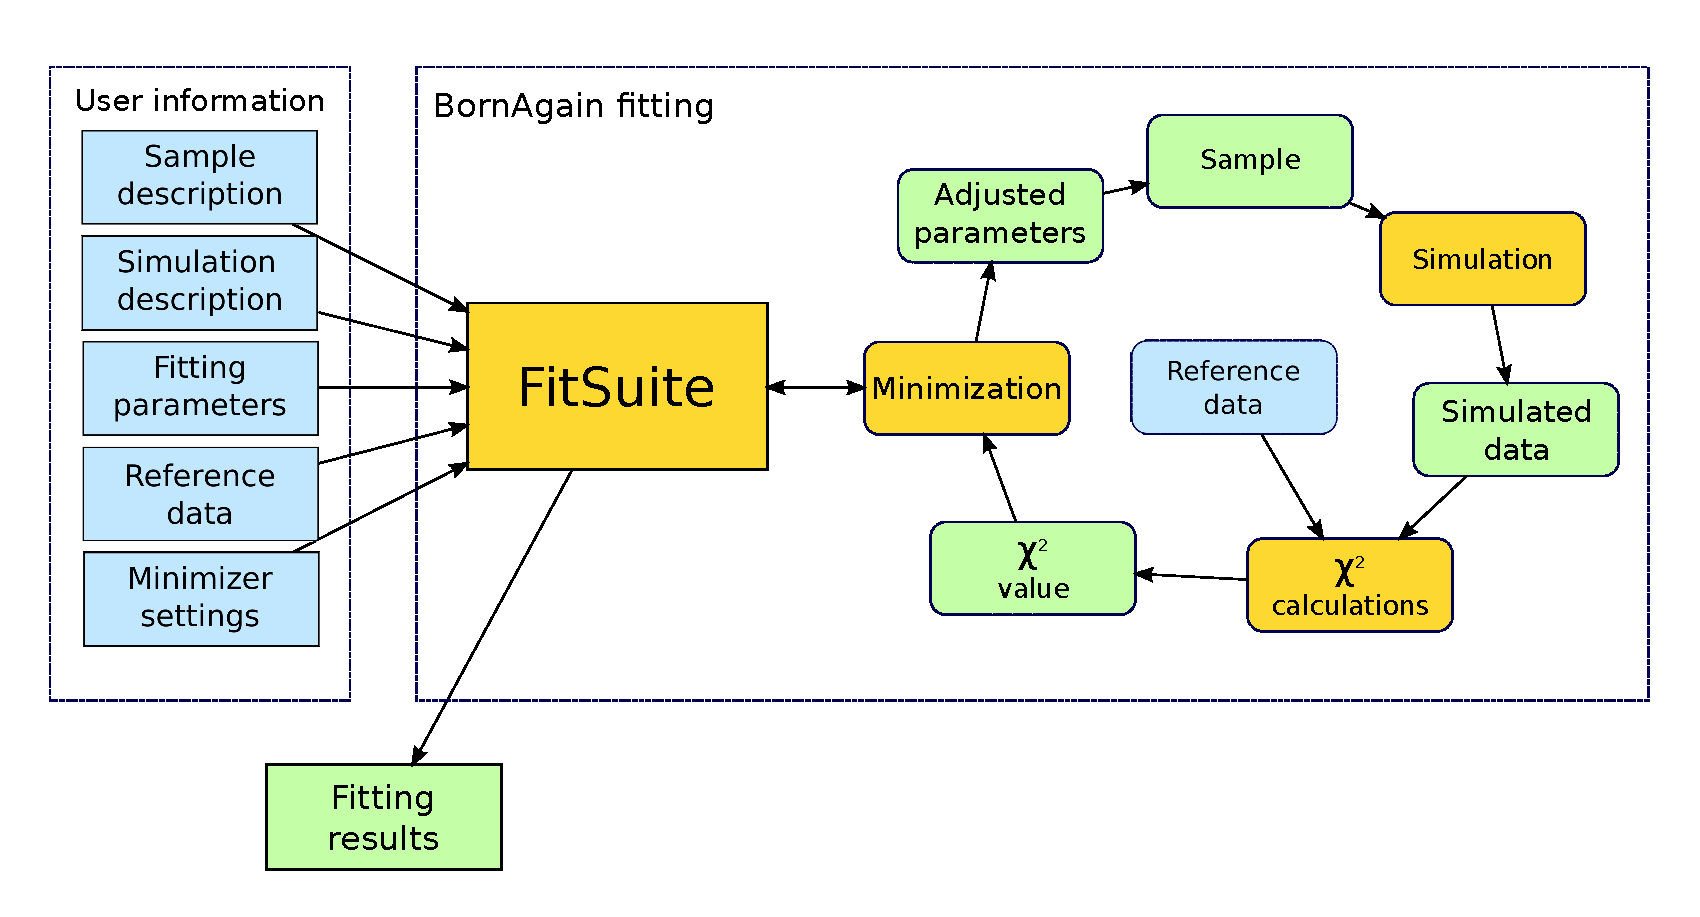
\includegraphics{Figures/minimization_workflow.eps}}
\caption{
Fitting work flow.
}
\label{fig:minimization_workflow}
\end{figure}

Before running the fitting the user is required to prepare some  data and to
configure the fitting kernel of \BornAgain\ . The required stages are

\begin{itemize}
\item Preparing the sample and the simulation description (multilayer, beam, detector parameters).
\item Choosing the fitting parameters.
\item Loading the reference data.
\item Defining the minimization settings.
\end{itemize}

The class \Code{FitSuite} contains the main functionalities to be used for the fit
and serves as the main interface between the user and the fitting work flow. 
The later involves iterations during which

\begin{itemize}
\item The minimizer makes an assumption about the optimal sample parameters.
\item These parameters are propagated to the sample.
\item The simulation is performed for the given state of the sample.
\item The simulated data (intensities) are propagated to the $\chi^2$ module.
\item The later calculates $\chi^2$ using the simulated and reference data.
\item The value of $\chi^2$ is propagated to the minimizer, which makes new assumptions about optimal sample parameters.
\end{itemize}

The iteration process is going on under the control of the selected minimization
algorithm, without any intervention from the
user. It stops 
\begin{itemize}
\item when the maximum number of iteration steps has been exceeded,
\item when the function's minimum has been reached within the tolerance window,
\item if the minimizer could not improve the values of the parameters. 
\end{itemize}

After the control is returned, fitting results can be retrieved.
They consist in the best $\chi^2$ value found, the corresponding
optimal sample parameters and the intensity map simulated with this set of parameters.

Details of \Code{FitSuite} class implementation and description
of each interface are given in \SecRef{FitSuiteClass}. The following parts of this section will detail each of
the main stages necessary to run a fitting procedure.


%%%%%%%%%%%%%%%%%%%%%%%%%%%%%%%%%%%%%%%%%%%%%%%%%%%%%%%%%%%%%%%%%%%%%%%%%%%%%%%
%
%%%%%%%%%%%%%%%%%%%%%%%%%%%%%%%%%%%%%%%%%%%%%%%%%%%%%%%%%%%%%%%%%%%%%%%%%%%%%%%
\subsection{Preparing the sample and the simulation description}

This step is similar for any simulation using \BornAgain\ (see \SecRef{Simulation}). It consists in first characterizing  the geometry of the system: the particles 
(shapes, sizes, refractive
indices), the different layers (thickness,
order, refractive index, a possible roughness of the interface), the
interference between the particles and the way they are distributed in
the layers (buried particles or particles sitting on top of a
layer). 
Then we specify the parameters of the input beam and of the
output detector.


%%%%%%%%%%%%%%%%%%%%%%%%%%%%%%%%%%%%%%%%%%%%%%%%%%%%%%%%%%%%%%%%%%%%%%%%%%%%%%%
%
%%%%%%%%%%%%%%%%%%%%%%%%%%%%%%%%%%%%%%%%%%%%%%%%%%%%%%%%%%%%%%%%%%%%%%%%%%%%%%%
\subsection{Choice of parameters to be fitted}
In principle, every parameter used in the construction of the sample
can be used as a fitting parameter. For example, the particles'
heights, radii or the layer's roughness or thickness could be selected
using the 
parameter pool mechanism. 
This mechanism is explained in detail in
\SecRef{WorkingWithSampleParameters} and it is therefore recommended
to read it before proceeding any further.

The user specifies selected sample parameters as fit parameters using \Code{FitSuite}
and its \Code{addFitParameter} method
\begin{lstlisting}[language=shell, style=commandline]
fit_suite = FitSuite()
fit_suite.addFitParameter(<name>, <initial value>, <step>, <limits>)
\end{lstlisting}
where \Code{<name>} corresponds to the parameter name in the sample's parameter pool.
By using wildcards in the parameter name, a group of sample parameters, corresponding to the given
pattern, can be associated with a single fitting parameter and 
fitted simultaneously to get a common optimal value (see \SecRef{WorkingWithSampleParameters}).

The second parameter \Code <initial value> correspond to the initial value of
the fitting parameter, while the third one
is responsible to the initial iteration steps size.
The last parameter \Code{<AttLimits>} corresponds to
the boundaries imposed on parameter value. It can be
\begin{itemize}
\item \Code{limitless()} by default, 
\item \Code{fixed()}, 
\item \Code{lowerLimited(<min\_value>)}, 
\item \Code{upperLimited(<max\_value>)}, 
\item \Code{limited(<min\_value>, <max\_value>)}.
\end{itemize}
where \Code{<min\_value>} and \Code{<max\_value>} are
double values corresponding to the lower and higher boundary, respectively.


%%%%%%%%%%%%%%%%%%%%%%%%%%%%%%%%%%%%%%%%%%%%%%%%%%%%%%%%%%%%%%%%%%%%%%%%%%%%%%%
%
%%%%%%%%%%%%%%%%%%%%%%%%%%%%%%%%%%%%%%%%%%%%%%%%%%%%%%%%%%%%%%%%%%%%%%%%%%%%%%%
\subsection{Associating reference and simulated data}

The minimization procedure deals with a pair of reference data (normally
associated with experimental data) and the theoretical model (presented by the sample and the simulation descriptions).

We assume that the experimental data are a two-dimensional intensity 
matrix as function of the output scattering
angles $\alpha_f$ and $\phi_f$ (see Fig.~\ref{fig:multil3d}).
The user is required to provide the data in the form of an ASCII file
containing an axes
binning description and the intensity data itself. 
\vspace*{2mm}

\ImportantPoint{Remark:}{
We recognize the importance of supporting the most common data formats. We are going to provide
this feature in the following releases and welcome users' requests on this subject.
}
\vspace*{1mm}

To associate the simulation and the reference data to the fitting engine, method \newline
\Code{addSimulationAndRealData} has to be used as shown
\begin{lstlisting}[language=python, style=eclipseboxed,numbers=none]
fit_suite = FitSuite()
fit_suite.addSimulationAndRealData(<simulation>, <reference>, <chi2_module>)
\end{lstlisting}

Here \Code{<simulation>} corresponds to a \BornAgain\ simulation object
with the  sample, beam and detector fully defined, \Code{<reference>}
corresponds to the experimental data object obtained from the ASCII file and \Code{<chi2\_module>} is an optional parameter for advanced 
control of $\chi2$ calculations.

It is possible to call this given method more than once to submit more than one pair of
\Code{<simulation>, <reference>} to the fitting procedure.
In this way, simultaneous fits of
some combined data sets are performed.

By using the third \Code{<chi2\_module>} parameter, different normalizations and weights
can be applied to give user full control of the way $\chi2$ is calculated.
This feature will be explained in \SecRef{FittingAdvanced}.


%%%%%%%%%%%%%%%%%%%%%%%%%%%%%%%%%%%%%%%%%%%%%%%%%%%%%%%%%%%%%%%%%%%%%%%%%%%%%%%
%
%%%%%%%%%%%%%%%%%%%%%%%%%%%%%%%%%%%%%%%%%%%%%%%%%%%%%%%%%%%%%%%%%%%%%%%%%%%%%%%
\subsection{Minimizer settings}

\BornAgain\ contains a variety of minimization engines from \Code{ROOT} and \Code{GSL}
libraries. They are listed in Table~\ref{table:fit_minimizers}.
By default \Code{Minuit2} minimizer with default settings will be used and no additional
configuration needs to be done.
The remainder of this section explains some of the expert settings, which can be applied to get better 
fit results.

The default minimization algorithm can be changed using 
\Code{MinimizerFactory} as shown below
\begin{lstlisting}[language=python, style=eclipseboxed,numbers=none]
fit_suite = FitSuite()
minimizer = MinimizerFactory.createMinimizer("<Minimizer name>","<algorithm>")
fit_suite.setMinimizer(minimizer)
\end{lstlisting}

where \Code{<Minimizer name>} and \Code{<algorithm>} can be chosen from the first and
second column of Table~\ref{table:fit_minimizers} respectively. 
The list of minimization algorithms implemented in \BornAgain\
can also be obtained using \Code{MinimizerFactory.printCatalogue()} command.


\begin{table}[h]
\centering
\begin{tabular}{@{}lll@{}}
\hline
\hline
\textbf{Minimizer name} & \textbf{Algorithm} & \textbf{Description}\\
\hline
\Code{Minuit2} \cite{MinuitURL} & \Code{Migrad} & According to
\cite{mntutorial} best minimizer for nearly all functions,\\
 & & variable-metric method with inexact line search, \\
 & & a stable metric updating scheme,\\
 & &  and checks for positive-definiteness.\\
\hline
                                       & \Code{Simplex} & simplex method of
                                       Nelder and Mead\\ 
 & & usually slower than \Code{Migrad}, \\
 &  & rather robust with respect to gross fluctuations in the\\ & &  function
 value, gives no reliable information about \\ & &  parameter errors, \\
\hline
                                       & \Code{Combined} & minimization with
                                       \Code{Migrad} \\
                                       & & but switches to Simplex if
                                       Migrad fails to converge.\\
\hline
                                       & \Code{Scan} &  not intended to
                                       minimize, just scans the
                                       function,\\
                                       & &  one parameter at a
                                       time, retains the best value
                                       after\\ &  & each scan\\
\hline
                                       & \Code{Fumili} & optimized
                                       method for least square and log
                                       likelihood\\ & &  minimizations \\
\hline
\Code{GSLMultiMin} \cite{GSLMultiMinURL} & \Code{ConjugateFR} & Fletcher-Reeves conjugate gradient
  algorithm,\\
\hline
& \Code{ConjugatePR} & Polak-Ribiere conjugate gradient algorithm,\\ 
\hline
& \Code{BFGS} & Broyden-Fletcher-Goldfarb-Shanno algorithm,\\ 
\hline
& \Code{BFGS2} & improved version of BFGS,\\ 
\hline
& \Code{SteepestDescent} & follows the downhill gradient of the function at each step\\
\hline
\Code{GSLMultiFit} \cite{GSLMultiFitURL} & & Levenberg-Marquardt
Algorithm\\
\hline
\Code{GSLSimAn} \cite{GSLSimAnURL}& & Simulated Annealing Algorithm\\ 
\hline
\hline
\end{tabular}
\caption{List of minimizers implemented in \BornAgain. }
\label{table:fit_minimizers}
\end{table}

There are several options common to every minimization algorithm, which can be changed
before starting the minimization. They are handled by \Code{MinimizerOptions} class:
\begin{lstlisting}[language=python, style=eclipseboxed, numbers = none]
options = MinimizerOptions()
options.setMaxFunctionCalls(10)
fit_suite.getMinimizer().setOptions(options)
\end{lstlisting}
In the above code snippet, a number of ``maximum function calls'',
namely the maximum number of times the minimizer is allowed to call the simulation, is limited to 10. %The minimizer will take that number into consideration and will try to limit number of iterations by that value.

There are also expert-level options common for all minimizers as well
as a number of options to tune individual minimization algorithms.
They will be explained in \SecRef{FittingAdvanced}.


%%%%%%%%%%%%%%%%%%%%%%%%%%%%%%%%%%%%%%%%%%%%%%%%%%%%%%%%%%%%%%%%%%%%%%%%%%%%%%%
%
%%%%%%%%%%%%%%%%%%%%%%%%%%%%%%%%%%%%%%%%%%%%%%%%%%%%%%%%%%%%%%%%%%%%%%%%%%%%%%%
\subsection{Running the fitting ant retrieving the results}

After the initial configuration of \Code{FitSuite} has been performed, the fitting
can be started using the command
\begin{lstlisting}[language=python, style=eclipseboxed, numbers = none]
fit_suite.runFit()
\end{lstlisting}

Depending on the complexity of the sample and the number of free sample parameters the fitting
process can take from tens to thousands of iterations. The results of the fit can
be printed on the screen using the command
\begin{lstlisting}[language=python, style=eclipseboxed, numbers = none]
fit_suite.printResults()
\end{lstlisting}
\SecRef{FittingExamples} gives more details about how to access the fitting results.




\section{Basic Python fitting example} \SecLabel{FittingExamples}

In this section we are going to go through a complete example of
fitting using \BornAgain. Each  step will be associated with a
detailed piece of code written in \Python. 
The complete listing of
the script is given in Appendix (see Listing~\ref{PythonFittingExampleScript}).
The script can also be found at
\begin{lstlisting}[language=shell, style=commandline]
./Examples/python/fitting/ex002_FitCylindersAndPrisms/FitCylindersAndPrisms.py
\end{lstlisting}

\noindent
This example uses the same sample geometry as in \SecRef{Example1Python}.
Cylindrical and
prismatic particles in equal proportion are deposited on a substrate layer, with no interference
between the particles. We consider the following parameters to be unkown
\begin{itemize}
\item the radius of cylinders,
\item the height of cylinders,
\item the length of the prisms' triangular basis,
\item the height of prisms.
\end{itemize}

Our reference data are a ``noisy'' two-dimensional intensity
map obtained from the simulation of the same geometry with a fixed
value of $5\,{\rm nm}$ for the height and radius of cylinders and for the
height of prisms which have a 10-nanometer-long side length. 
Then we run our fitting using default minimizer settings
starting with a cylinder's height
of $4\,{\rm nm}$, a cylinder's radius of $6\,{\rm nm}$, 
a prism's half side of $6\,{\rm nm}$ and a height equal to $4\,{\rm nm}$.
As a result, the fitting procedure is able to find the correct value of $5\,{\rm nm}$
for all four parameters.


%%%%%%%%%%%%%%%%%%%%%%%%%%%%%%%%%%%%%%%%%%%%%%%%%%%%%%%%%%%%%%%%%%%%%%%%%%%%%%%
\subsubsection*{Importing Python libraries}
\begin{lstlisting}[language=python, style=eclipseboxed]
from libBornAgainCore import *
from libBornAgainFit import *
\end{lstlisting}
We start from importing two \BornAgain\ libraries required to create
the sample description
and to run the fitting.


%%%%%%%%%%%%%%%%%%%%%%%%%%%%%%%%%%%%%%%%%%%%%%%%%%%%%%%%%%%%%%%%%%%%%%%%%%%%%%%
\subsubsection*{Building the sample}
\begin{lstlisting}[language=python, style=eclipseboxed, firstnumber=5]
def get_sample(): @\label{script2::get_sample}@
    """
    Build the sample representing cylinders and pyramids on top of substrate without interference.
    """
    # defining materials
    m_air = HomogeneousMaterial("Air", 0.0, 0.0)
    m_substrate = HomogeneousMaterial("Substrate", 6e-6, 2e-8)
    m_particle = HomogeneousMaterial("Particle", 6e-4, 2e-8)

    # collection of particles
    cylinder_ff = FormFactorCylinder(1.0*nanometer, 1.0*nanometer)
    cylinder = Particle(m_particle, cylinder_ff)
    prism_ff = FormFactorPrism3(2.0*nanometer, 1.0*nanometer)
    prism = Particle(m_particle, prism_ff)
    particle_layout = ParticleLayout()
    particle_layout.addParticle(cylinder, 0.0, 0.5)
    particle_layout.addParticle(prism, 0.0, 0.5)
    interference = InterferenceFunctionNone()
    particle_layout.addInterferenceFunction(interference)

    # air layer with particles and substrate form multi layer
    air_layer = Layer(m_air)
    air_layer.setLayout(particle_layout)
    substrate_layer = Layer(m_substrate)
    multi_layer = MultiLayer()
    multi_layer.addLayer(air_layer)
    multi_layer.addLayer(substrate_layer)
    return multi_layer
\end{lstlisting}
The function starting at line~\ref{script2::get_sample} creates a multilayered sample
with cylinders and prisms using arbitrary $1\,{\rm nm}$ value for all size's of particles.
The details about the generation of this multilayered sample are given in \SecRef{Example1Python}.


%%%%%%%%%%%%%%%%%%%%%%%%%%%%%%%%%%%%%%%%%%%%%%%%%%%%%%%%%%%%%%%%%%%%%%%%%%%%%%%
\subsubsection*{Creating the simulation}
\begin{lstlisting}[language=python, style=eclipseboxed, firstnumber=35]
def get_simulation(): @\label{script2::get_simulation}@
    """
    Create GISAXS simulation with beam and detector defined
    """
    simulation = Simulation()
    simulation.setDetectorParameters(100, -1.0*degree, 1.0*degree, 100, 0.0*degree, 2.0*degree)
    simulation.setBeamParameters(1.0*angstrom, 0.2*degree, 0.0*degree)
    return simulation
\end{lstlisting}
The function starting at line~\ref{script2::get_simulation} creates
the simulation object with the definition of the beam and detector parameters.



%%%%%%%%%%%%%%%%%%%%%%%%%%%%%%%%%%%%%%%%%%%%%%%%%%%%%%%%%%%%%%%%%%%%%%%%%%%%%%%
\subsubsection*{Preparing the fitting pair}
\begin{lstlisting}[language=python, style=eclipseboxed, firstnumber=45]
def run_fitting(): @\label{script2::run_fitting}@
    """
    run fitting
    """
    sample = get_sample() @\label{script2::setup_simulation1}@
    simulation = get_simulation()
    simulation.setSample(sample) @\label{script2::setup_simulation2}@

    real_data = IntensityDataIOFactory.readIntensityData('refdata_fitcylinderprisms.txt') @\label{script2::real_data}@
\end{lstlisting}
Lines
~\ref{script2::setup_simulation1}-~\ref{script2::setup_simulation2}
generate the 
sample and simulation description and assign the sample to the simulation.
Our reference data are contained in the file \Code{'refdata\_fitcylinderprisms.txt'}.
 This reference had been generated by adding noise
on the scattered intensity from a numerical sample with a fixed length of 5~nm for the four fitting
parameters (\textit{i.e.} the dimensions of the cylinders and prisms).
Line ~\ref{script2::real_data} creates the real data object by loading
the ASCII data from the input file.


%%%%%%%%%%%%%%%%%%%%%%%%%%%%%%%%%%%%%%%%%%%%%%%%%%%%%%%%%%%%%%%%%%%%%%%%%%%%%%%
\subsubsection*{Setting up \rm\bf{FitSuite}}
\begin{lstlisting}[language=python, style=eclipseboxed, firstnumber=55]
    fit_suite = FitSuite() @\label{script2::fitsuite1}@
    fit_suite.addSimulationAndRealData(simulation, real_data) @\label{script2::fitsuite2}@
    fit_suite.initPrint(10) @\label{script2::fitsuite3}@
\end{lstlisting}
Line ~\ref{script2::fitsuite1} creates a \Code{FitSuite} object which provides
the main interface to the minimization kernel of \BornAgain\ . 
Line ~\ref{script2::fitsuite2} submits simulation description and real data pair to the 
subsequent fitting. Line ~\ref{script2::fitsuite3} sets up \Code{FitSuite} to print on
the screen the information about fit progress once per 10 iterations.
\begin{lstlisting}[language=python, style=eclipseboxed, firstnumber=60]
    fit_suite.addFitParameter("*FormFactorCylinder/height", 4.*nanometer, 0.01*nanometer, AttLimits.lowerLimited(0.01)) @\label{script2::fitpars1}@
    fit_suite.addFitParameter("*FormFactorCylinder/radius", 6.*nanometer, 0.01*nanometer, AttLimits.lowerLimited(0.01))
    fit_suite.addFitParameter("*FormFactorPrism3/height", 4.*nanometer, 0.01*nanometer, AttLimits.lowerLimited(0.01))
    fit_suite.addFitParameter("*FormFactorPrism3/length", 12.*nanometer, 0.02*nanometer, AttLimits.lowerLimited(0.01)) @\label{script2::fitpars2}@
\end{lstlisting}
Lines ~\ref{script2::fitpars1}--~\ref{script2::fitpars2} enter the
list of fitting parameters. Here we use the cylinders' height and
radius and the prisms' height and side length. 
The cylinder's length and prism half side are initially equal to $4\,{\rm nm}$,
whereas the cylinder's radius and the prism half side length are equal to $6\,{\rm nm}$ before the minimization. The
iteration step is equal to $0.01\,{\rm nm}$ and only the lower
boundary is imposed to be equal to $0.01\,{\rm nm}$.


%%%%%%%%%%%%%%%%%%%%%%%%%%%%%%%%%%%%%%%%%%%%%%%%%%%%%%%%%%%%%%%%%%%%%%%%%%%%%%%
\subsubsection*{Running the fit and accessing results}
\begin{lstlisting}[language=python, style=eclipseboxed, firstnumber=66]
    fit_suite.runFit() @\label{script2::fitresults1}@

    print "Fitting completed."
    fit_suite.printResults()@\label{script2::fitresults2}@
    print "chi2:", fit_suite.getMinimizer().getMinValue() 
    fitpars = fit_suite.getFitParameters()
    for i in range(0, fitpars.size()):
        print fitpars[i].getName(), fitpars[i].getValue(), fitpars[i].getError() @\label{script2::fitresults3}@
\end{lstlisting}
Line ~\ref{script2::fitresults1} shows the command to start the fitting process.
During the fitting the progress will be displayed on the screen.
Lines ~\ref{script2::fitresults2}--~\ref{script2::fitresults3} shows different ways of
accessing the fit results.


More details about fitting, access to its results and visualization of
the fit progress using matplotlib libraries can be learned from the
following detailed example
\begin{lstlisting}[language=shell, style=commandline]
./Examples/python/fitting/ex002_FitCylindersAndPrisms/FitCylindersAndPrisms_detailed.py
\end{lstlisting}



\section {Advanced fitting.} \SecLabel{FittingAdvanced}

\subsection{Affecting $\chi2$ calculations.}
\subsection{Simultaneous fit of several data sets.}
\subsection{Using fitting strategies.}
\subsection{Masking the real data.}
\subsection{Tuning fitting algorithms.}
\subsection{Fitting with correlated sample parameters.}



\section {How to get right answer from fitting.} 
\SecLabel{FittingRightAnswers}

As it was already mentioned in \SecRef{FittingGentleIntroducion}, 
one of the main difficulties in fitting the data with the model 
is the presence of multiple
local minima in the objective function. The extended list of problems causing fit to failure includes
\begin{itemize}
\item unreliable physical model
\item multiple local minima
\item unphysical behavior of objective function, unphysical regions in parameter space
\item unreliable parameter error calculation in the presence of limits on parameter value
\item often exponential behavior of objective function and corresponding numerical inaccuracies and excessive numerical roundoff in calculation of its value and derivatives
\item large correlations between parameters
\item very different scale of parameters involved in calculation
\item not positive definite error matrix even at minimum
\end{itemize}


Given list, of course, is unrelated only to \BornAgain\ fitting. It remains the same
while fitting the data with any fitting program and any kind of theoretical model.
To address all these difficulties some amount of manual tuning might be necessary. Below we give some recommendations which might help the user to achieve reliable fit results.

\subsection*{General recommendation}
\begin{itemize}
\item initially choose small number of free fitting parameters
\item eliminate redundand parameters
\item provide a good initial guess for fit parameters
\item start from default minimizer settings and turn to the fine tuning after some experience has been acquired.
\item repeat fit using different starting values for parameters or their limits
\item repeat fit fixing and releasing different groups  of parameters
\item use \Code{Minuit2} minimizer with \Code{Migrad} algorithm (default) to get most reliable parameter error estimation
\item try \Code{GSLMultiFit} minimizer or \Code{Minuit2} minimizer with \Code{Fumili} algorithm to get fewer iterations


%\subsection*{Interpretation of errors.}


{\bf to be continued... }


\end{itemize}





%%%%%%%%%%%%%%%%%%%%%%%%%%%%%%%%%%%%%%%%%%%%%%%%%%%%%%%%%%%%%%%%%%%%%%%%%%%%%%%%%
\section{User API} \label{UserAPI}
%%%%%%%%%%%%%%%%%%%%%%%%%%%%%%%%%%%%%%%%%%%%%%%%%%%%%%%%%%%%%%%%%%%%%%%%%%%%%%%%

%===============================================================================
\subsection{IntensityData}
%===============================================================================

The \Code{IntensityData} object stores the
simulated or real intensity data together with the axes definition of the detector in BornAgain's internal format.
During the simulation setup
it is created automatically when the user specifies the detector characteristics and is filled with the simulated intensities after the simulation is completed.

\begin{lstlisting}[language=python, style=eclipseboxed]
simulation = Simulation()
simulation.setDetectorParameters(10, -5.0*degree, 5.0*degree, 5, 0.0*degree, 1.0*degree)
...
simulation.runSimulation()
intensity = simulation.getIntensityData() @\label{py:UserApi:intensity}@
\end{lstlisting}

The \Code{IntensityData} object retrieved in line~\ref{py:UserApi:intensity} corresponds to
the two dimensional detector pixel array as shown in \cref{fig:UserApi:IntensityData}.

\begin{figure}[ht]
  \centering
    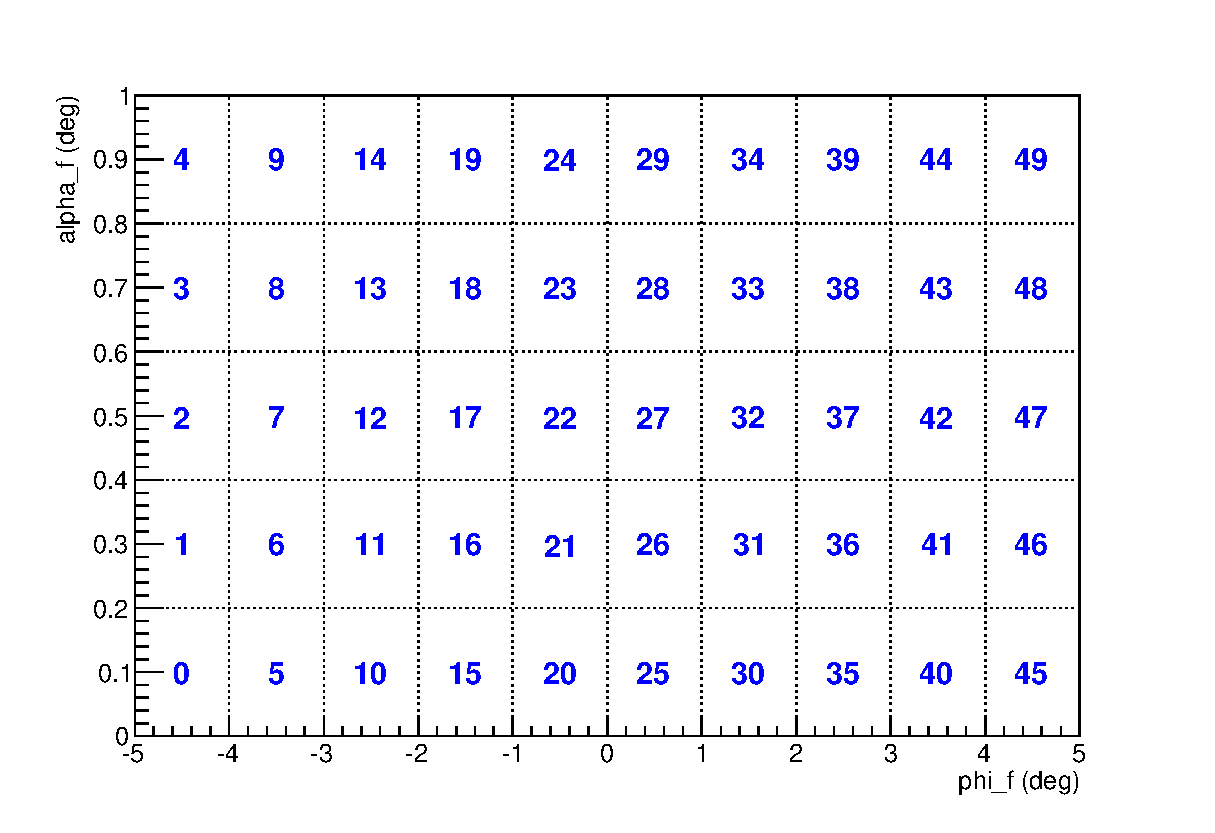
\includegraphics[clip=, width=120mm]{fig/drawing/UserAPI_IntensityDataLayout.eps}
  \caption{The axes layout of IntensityData object.}
  \label{fig:UserApi:IntensityData}
\end{figure}

The x-axis and y-axis of the figure correspond to the $\phi_f$ and $\alpha_f$ axes of the detector.
The x-axis is divided into 10 bins,
with low edge of the first bin set to $-5.0\,{\rm deg}$ and upper edge of the last bin set to $+5.0\,{\rm deg}$.
The y-axis is divided into 5 bins,
with low edge of the first bin set to $0.0\,{\rm deg}$ and upper edge of the last bin set to $1.0\,{\rm deg}$.
There are 50 bins in total (they are marked on the plot with indexes from 0 to 49), each bin will contain one intensity value.

During a standard simulation (i.e. no Monte-Carlo integration involved) intensities are calculated for $\phi_f, \alpha_f$ values corresponding to the bin centers, e.g. the intensity stored in bin\#42 will correspond to $\phi_f=3.5\,{\rm deg}, \alpha_f=0.5\,{\rm deg}$.
\vspace*{2mm}


\MakeRemark{}{
The \Code{IntensityData} object is not intended for direct usage from Python API. The idea is
that the API provides the user with the possibility to export the data from BornAgain internal format to the format of his choice as well as import user's data into BornAgain.
For the moment this functionality is limited to a few options explained below.
We encourage users feedback to implement the support of most requested formats.
}\\



\subsubsection{Import/export of intensity data}
For the moment we provide following options:
\begin{itemize}
\item Import/export of \Code{IntensityData} object from/to \Code{numpy} array.
\item Import/export of \Code{IntensityData} object from/to text file.

\end{itemize}

\paragraph{Export to numpy array}

To export intensity data into  \Code{numpy} array the method \Code{getArray()} should be used
on \Code{IntensityData} object as shown in line \ref{py:UserApi:getArray} of
following code snippet.

\begin{lstlisting}[language=python, style=eclipseboxed]
intensity = simulation.getIntensityData()
array = intensity.getArray() @\label{py:UserApi:getArray}@
...
pylab.imshow(numpy.rot90(array, 1)) @\label{py:UserApi:imshow}@
pylab.show()
\end{lstlisting}

For the detector settings defined in the previous paragraph the dimensions of the resulting array will be (10,5). By using \Code{numpy} indexes the user can get access to the intensity values, e.g.
\Code{array[0][0]} corresponds to the intensity in bin\#0 of \cref{fig:UserApi:IntensityData},
\Code{array[0][4]} to bin\#4,
\Code{array[1][0]} to bin\#5,
\Code{array[8][2]} to bin\#42,
\Code{array[9][4]} to bin\#49.


To plot this resulting numpy array with \Code{matplotlib} it has to be rotated counter-clockwise
to match \Code{matplotlib} conventions as shown in line~\ref{py:UserApi:imshow}.


%\subsubsection{Direct access to the data}
%User can access to the

%\begin{lstlisting}[language=python, style=eclipseboxed]
%for i in range(0, intensity.getAllocatedSize()):
%    print intensity[i]
%\end{lstlisting}


\subsubsection{Importing from numpy array}

To use fitting the user has to load experimental data into BornAgain fitting kernel.
To read experimental data the user has to create
IntensityData object, fill it with the experimental  intensity values and pass
this object to the fitting kernel.

First, the user creates empty \Code{IntensityData} as shown
in line~\ref{py:UserApi:IntensityData} of the following code snippet.
\begin{lstlisting}[language=python, style=eclipseboxed]
data = IntensityData() @\label{py:UserApi:IntensityData}@
data.addAxis(FixedBinAxis("phi_f", 10, -5.0*degree, 5.0*degree)) @\label{py:UserApi:phi_f}@
data.addAxis(FixedBinAxis("alpha_f", 5, 0.0*degree, 1.0*degree)) @\label{py:UserApi:alpha_f}@
...
array = numpy.zeros((10, 5)) # fill array with experimental intensities @\label{py:UserApi:create_array}@
...
data.setRawDataVector(array.flatten().tolist()) @\label{py:UserApi:set_raw}@

fitSuite = FitSuite() @\label{py:UserApi:fit_suite}@
fitSuite.addSimulationAndRealData(simulation, data) @\label{py:UserApi:add_real_data}@
\end{lstlisting}

In lines~\ref{py:UserApi:phi_f}, \ref{py:UserApi:alpha_f} two axes with fixed bin sizes
are defined to represent the detector layout as shown in \cref{fig:UserApi:IntensityData}.
The constructor of \Code{FixedBinAxis} object has the following signature

\begin{lstlisting}[language=python, style=eclipse,numbers=none]
FixedBinAxis(title, nbins, min_angle, max_angle)
\end{lstlisting}

The created \Code{IntensityData} object has to be filled with experimental intensities
using \Code{numpy} array prepared by the user (lines ~\ref{py:UserApi:create_array}-~\ref{py:UserApi:set_raw}). In lines \ref{py:UserApi:fit_suite},\ref{py:UserApi:add_real_data} the fitting kernel is created and initialized with \Code{Simulation} object and
\Code{IntensityData} object representing the experimental data.


\subsubsection{Saving intensity data to text file.}

The special class \Code{IntensityDataIOFactory} is intended for saving the intensity data
in different datafile formats. For the moment, it only supports saving the data in specific BornAgain's text files (the file extention \Code{*.int}).

\begin{lstlisting}[language=python, style=eclipseboxed]
intensity = simulation.getIntensityData()
IntensityDataIOFactory.writeIntensityData(intensity, 'file_name.int')
\end{lstlisting}

\subsubsection{Reading intensity data from a text file.}
The same class is also intended for reading intensity data
from files with different formats. For the moment, it only supports reading the data from text files of special BornAgain's format (the file extention \Code{*.int}).

\begin{lstlisting}[language=python, style=eclipseboxed]
intensity = IntensityDataIOFactory.readIntensityData('file_name.int')
\end{lstlisting}


%%%%%%%%%%%%%%%%%%%%%%%%%%%%%%%%%%%%%%%%%%%%%%%%%%%%%%%%%%%%%%%%%%%%%%%%%%%%%%%%
%%
%%   BornAgain User Manual
%%
%%   homepage:   http://www.bornagainproject.org
%%
%%   copyright:  Forschungszentrum Jülich GmbH 2015
%%
%%   license:    Creative Commons CC-BY-SA
%%   
%%   authors:    Scientific Computing Group at MLZ Garching
%%               C. Durniak, M. Ganeva, G. Pospelov, W. Van Herck, J. Wuttke
%%
%%%%%%%%%%%%%%%%%%%%%%%%%%%%%%%%%%%%%%%%%%%%%%%%%%%%%%%%%%%%%%%%%%%%%%%%%%%%%%%%


\chapter{Particle form factors}  \label{SFF}

\makeatletter
\renewcommand{\@thesubfigure}{\relax}
\makeatother

\index{Form factor|(}

%%%%%%%%%%%%%%%%%%%%%%%%%%%%%%%%%%%%%%%%%%%%%%%%%%%%%%%%%%%%%%%%%%%%%%%%%%%%%%%%
\section{Shape transforms}
%%%%%%%%%%%%%%%%%%%%%%%%%%%%%%%%%%%%%%%%%%%%%%%%%%%%%%%%%%%%%%%%%%%%%%%%%%%%%%%%

\index{Shape transform|(}
The form factor of a particle is the Fourier transform
of its shape function,
\begin{equation}
  F(\q)=\int {\rm d}^3r\, {\rm e}^{i\q\r} S(\r).
\end{equation}
For hard-shell particles the shape function $S(\r)$
only takes the values 0 and~1
so that the form factor becomes
the \textit{shape transform}
\begin{equation}\label{eq:FFHard}
  F(\q)=\int_V {\rm d}^3r\, {\rm e}^{i\q\r},
\end{equation}
where $V$ is the volume of the particle.
\nomenclature[2v130 0]{$V$}{Volume of embedded particle}%

\BornAgain\ comes with a collection of hard-coded 
shape transform for standard particle geometries like
spheres, cylinders, prisms, pyramids or ripples.
This collection is documented in the following.
For each shape,
the real-space geometry is shown in orthogonal projections,
the parameters of the \BornAgain\ method are defined,
an analytical expression for the form factor is given,
and exemplary results for $\left|F(\q)\right|^2$ versus
$\alpha_\tf,\phi_\tf$ are shown for small-angle scattering conditions
($\alpha_\ti=\phi_\ti=0$).

The computation of $F(\q)$ is based on
shapes $S(\r)$ given in Cartesian coordinates,
as defined in the orthogonal projections.
Typically, the vertical ($z$) direction is chosen
along a symmetry axis of the particle.
The origin is always at the center of the bottom side of the particle.
Different parametrization or a different choice of the origin
cause our analytic form factors to trivially deviate
from expressions given in the \IsGISAXS\ manual \cite[Sect.~2.3]{Laz08}
or in the literature \cite[Appendix]{ReLL09}.

We recomputed all expressions to make sure
that they also hold for complex scattering vectors,
used to describe in order to take any material absorption into account.
The implementation in \BornAgain\ allows all three components
of~$\q$ to be complex.
According to Sect.~\ref{Smulayabs},
only the vertical components of $\k_\ti$ and $\k_\tf$ can have imaginary parts.
However,
to account for a tilt of the particle,
it may be necessary to evaluate $F(\v{\tilde q})$ with
a rotated scattering vector~$\v{\tilde q}$
that has complex $\tilde q_x$ or~$\tilde q_y$.

\E{Ripples}
\index{Ripple (form factor)}%
 are particles with infinite extension in one dimension
(by convention in $x$ direction).
They have the shape transform 
\begin{equation}\label{eq:FFHard}
  F(\q)=\delta(q_x)\int_A {\rm d}^2r\, {\rm e}^{i(q_x x+q_y y)},
\end{equation}
where $A$ is the cross section.
To avoid an extra distinction of cases,
\BornAgain\ requests that ripples have a \E{finite} length~$L$,
which users may keep fixed at a very large value.

The following tables summarize the implemented particle geometries,
 ordered by ascending number of parameters.
Afterwards, the detailed documentation is in alphabetical order.

\def\entry#1#2#3#4{%
\raisebox{-3.8ex}{\includegraphics[width=5em]{fig/blue/#2.png}} &
\texttt{#1} &
#4 &
Page~\pageref{sec:#3}, Sect.~\ref{sec:#3}\\}
\begin{center}
\small
\begin{longtable}
  {@{}p{.15\textwidth}
   @{}p{.35\textwidth}
   @{}p{.2\textwidth}
   @{}p{.25\textwidth}@{}}
Shape&Name&Parameters&Reference\\\hline
\entry{FullSphere}{FullSphere3d}{FullSphere}{$R$}
\hline
\entry{FullSpheroid}{FullSpheroid3d}{FullSpheroid}{$R$, $H$}
\entry{TruncatedSphere}{Sphere3d}{TruncatedSphere}{$R$, $H$}
\entry{Cylinder}{Cylinder3d}{Cylinder}{$R$, $H$}
\entry{Prism3}{Prism33d}{Prism3}{$L$, $H$}
\entry{Prism6}{Prism63d}{Prism6}{$R$, $H$}
\entry{TruncatedCube}{TruncatedCube3d}{TruncatedCube}{$L$, $t$}
\hline
\entry{EllipsoidalCylinder}{EllipsoidalCylinder3d}{EllipsoidalCylinder}{$R_a$, $R_b$, $H$}
\entry{HemiEllipsoid}{HemiEllipsoid3d}{HemiEllipsoid}{$R_a$, $R_b$, $H$}
\entry{TruncatedSpheroid}{Spheroid3d}{TruncatedSpheroid}{$R$, $H$, $f_p$}
\entry{Cone}{Cone3d}{Cone}{$R$, $H$, $\alpha$}
\entry{Box}{Box3d}{Box}{$L$, $W$, $H$}
\entry{Pyramid}{Pyramid3d}{Pyramid}{$L$, $H$, $\alpha$}
\entry{Tetrahedron}{Tetrahedron3d}{Tetrahedron}{$L$, $H$, $\alpha$}
\entry{Cone6}{Cone63d}{Cone6}{$R$, $H$, $\alpha$}
\entry{Ripple1}{Ripple13d}{Ripple1}{$L$, $W$, $H$}
\hline
\entry{AnisoPyramid}{AnistropicPyramid3d}{AnisoPyramid}{$L$, $W$, $H$, $\alpha$}
\entry{Cuboctahedron}{Cuboctahedron3d}{Cuboctahedron}{$L$, $H$, $r_H$, $\alpha$}
\entry{Ripple2}{Ripple23d}{Ripple2}{$L$, $W$, $H$, $d$}
\hline
\end{longtable}
\end{center}

In the following subsections,
information about the implemented geometries is given in standardized form.
Analytical expressions are given for the form factor $F(\q)$,
for the volume $V=F(0)$,
and for the maximum horizontal section $S$
(the area of the particle as seen from above).
\nomenclature[2s130 0]{$S$}{Maximum horizontal section of embedded particle}%
Mathematical notation in the form factor expressions includes
the cardinal sine functions $\sinc(z)\coloneqq\sin(z)/z$
and the Bessel function of first kind and first order $J_1(z)$
\cite[Ch.~9]{AbSt64}.
\nomenclature[2j132 01]{$J_1$}{Bessel function of first kind and first order}%
If results contain an integral,
then no analytical form was found,
and the integral is evaluated by numeric quadrature.
\index{Quadrature}%
The analytical expressions for $F(\q)$ contain singularities for
certain values of $\q$.
All these singularities are removable.
Our implementation comprises appropriate case distinctions.

Geometrical objects can be parametrized in different ways.
Concerns about user experience and about code readability
sometimes lead to different choices.
For the \BornAgain\ user interfaces (GUI and API)
we have chosen the most standard parameters,
as used in elementary geometry, like length, height, radius,
even if this is at variance from the \IsGISAXS\ precedent.
Where our parametrization made analytic expressions too tedious,
we use alternate internal parameters to alleviate the formul\ae.

Examplary form factors are numerically computed in Born approximation.
The particles are assigned a refractive index of $n=10^{-5}$.
Parameters are chosen such that within $\pm5$~\%
the particle volume~$V$ is 250~nm$^3$.
The incident wavelength is 1~\AA.
The incident beam is always in $x$ direction, hence $\alpha_\ti=\phi_\ti=0$.
Simulated detector images are normalized to the maximum scattering intensity at $F(0)=V$.
All plots of $|F(q)|^2/V^2$ versus $\alpha_\tf$ and $\phi_\tf$
are shown for the same angular range $0\ldots5^\circ$
and on the same logarithmic color scale.

%-------------------------------------------------------------------------------
% Start the series of standardized double pages.
\ifodd\value{page}\else\FloatBarrier\newpage\textit{Page intentionally left blank}\fi
%-------------------------------------------------------------------------------

%-------------------------------------------------------------------------------
\FloatBarrier\newpage
\subsection{AnisoPyramid (rectangle-based)} \label{sec:AnisoPyramid} 
  \index{Anisotropic pyramid (form factor)}
  \index{Pyramid (form factor)!rectangular (AnisoPyramid)}
  \index{Truncated pyramid (form factor)!rectangular (AnisoPyramid)}
  \index{FormFactorAnisoPyramid@\Code{FormFactorAnisoPyramid}}
%-------------------------------------------------------------------------------

\paragraph{Real-space geometry}\strut\\

\begin{figure}[H]
\hfill
\subfigure[Perspective]{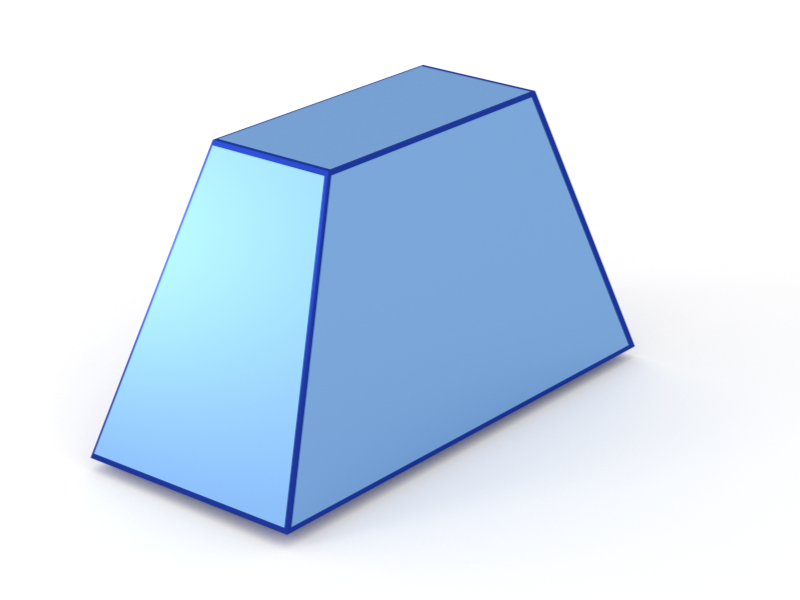
\includegraphics[width=.24\textwidth]{fig/blue/AnistropicPyramid3d.png}}
\hfill
\subfigure[Top view]{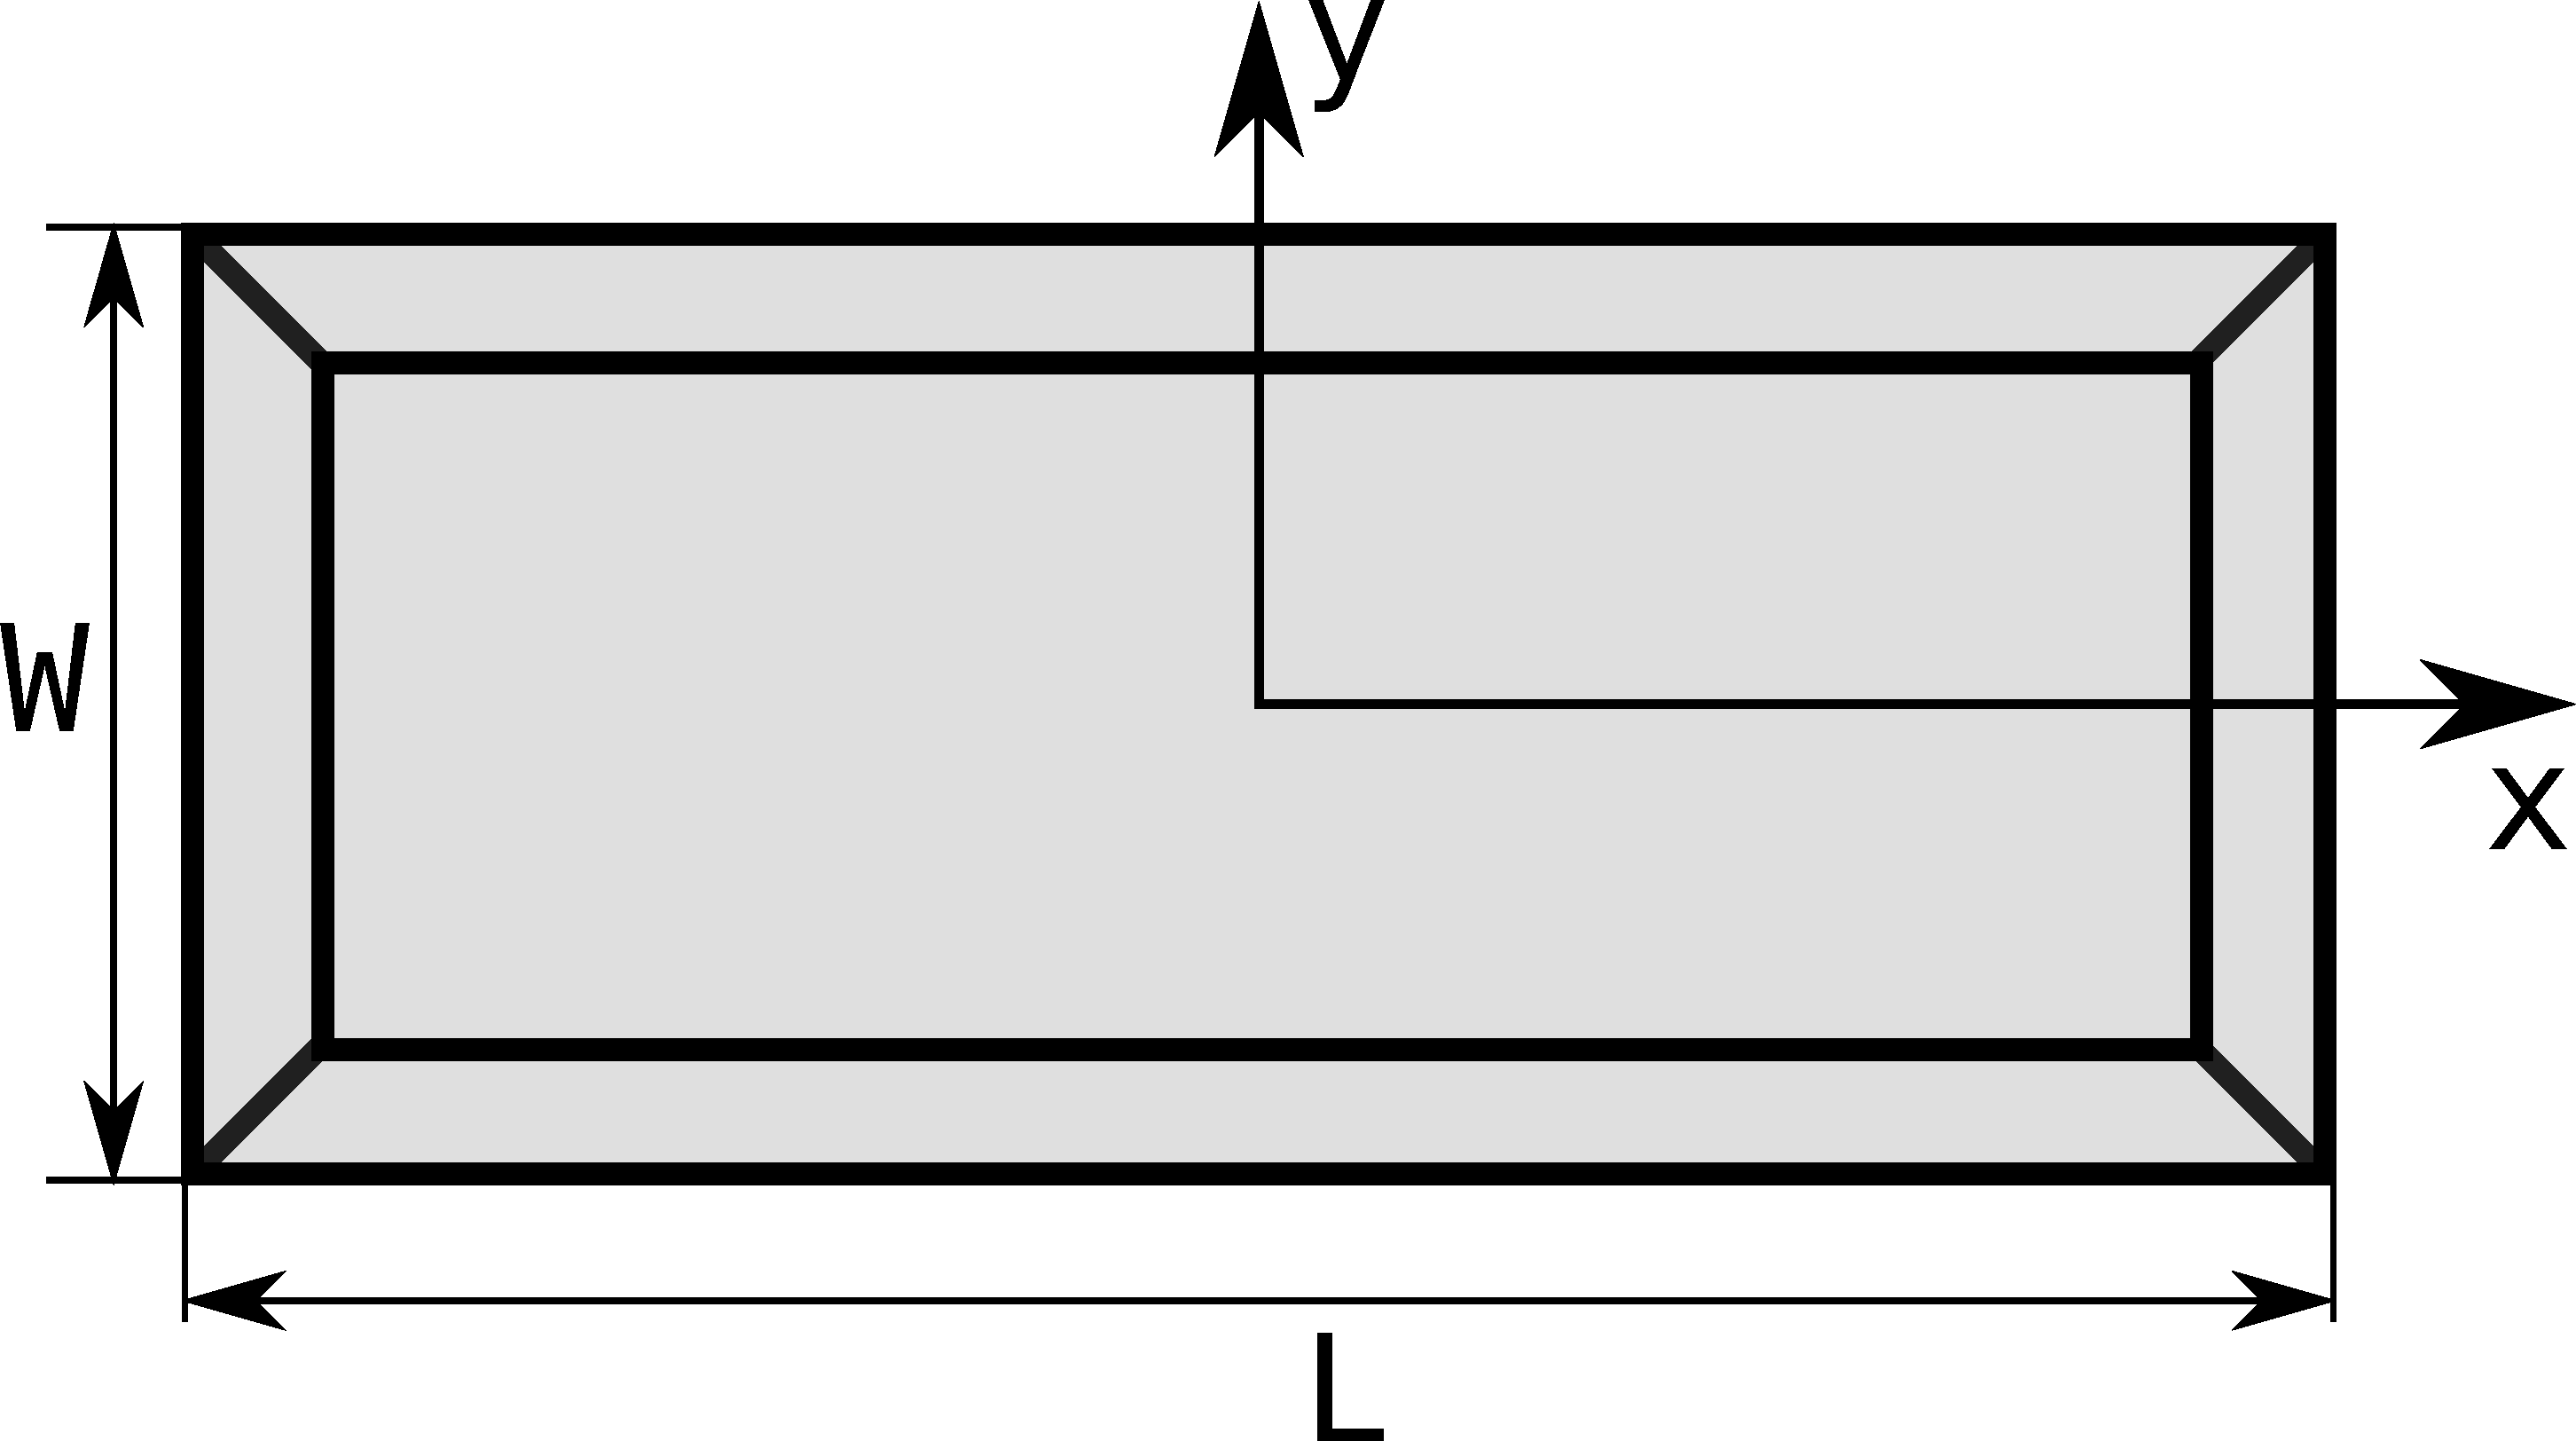
\includegraphics[width=.30\textwidth]{fig/cuts/AnisoPyramid2dxy.pdf}}
\hfill
\subfigure[Side view]{\raisebox{2mm}{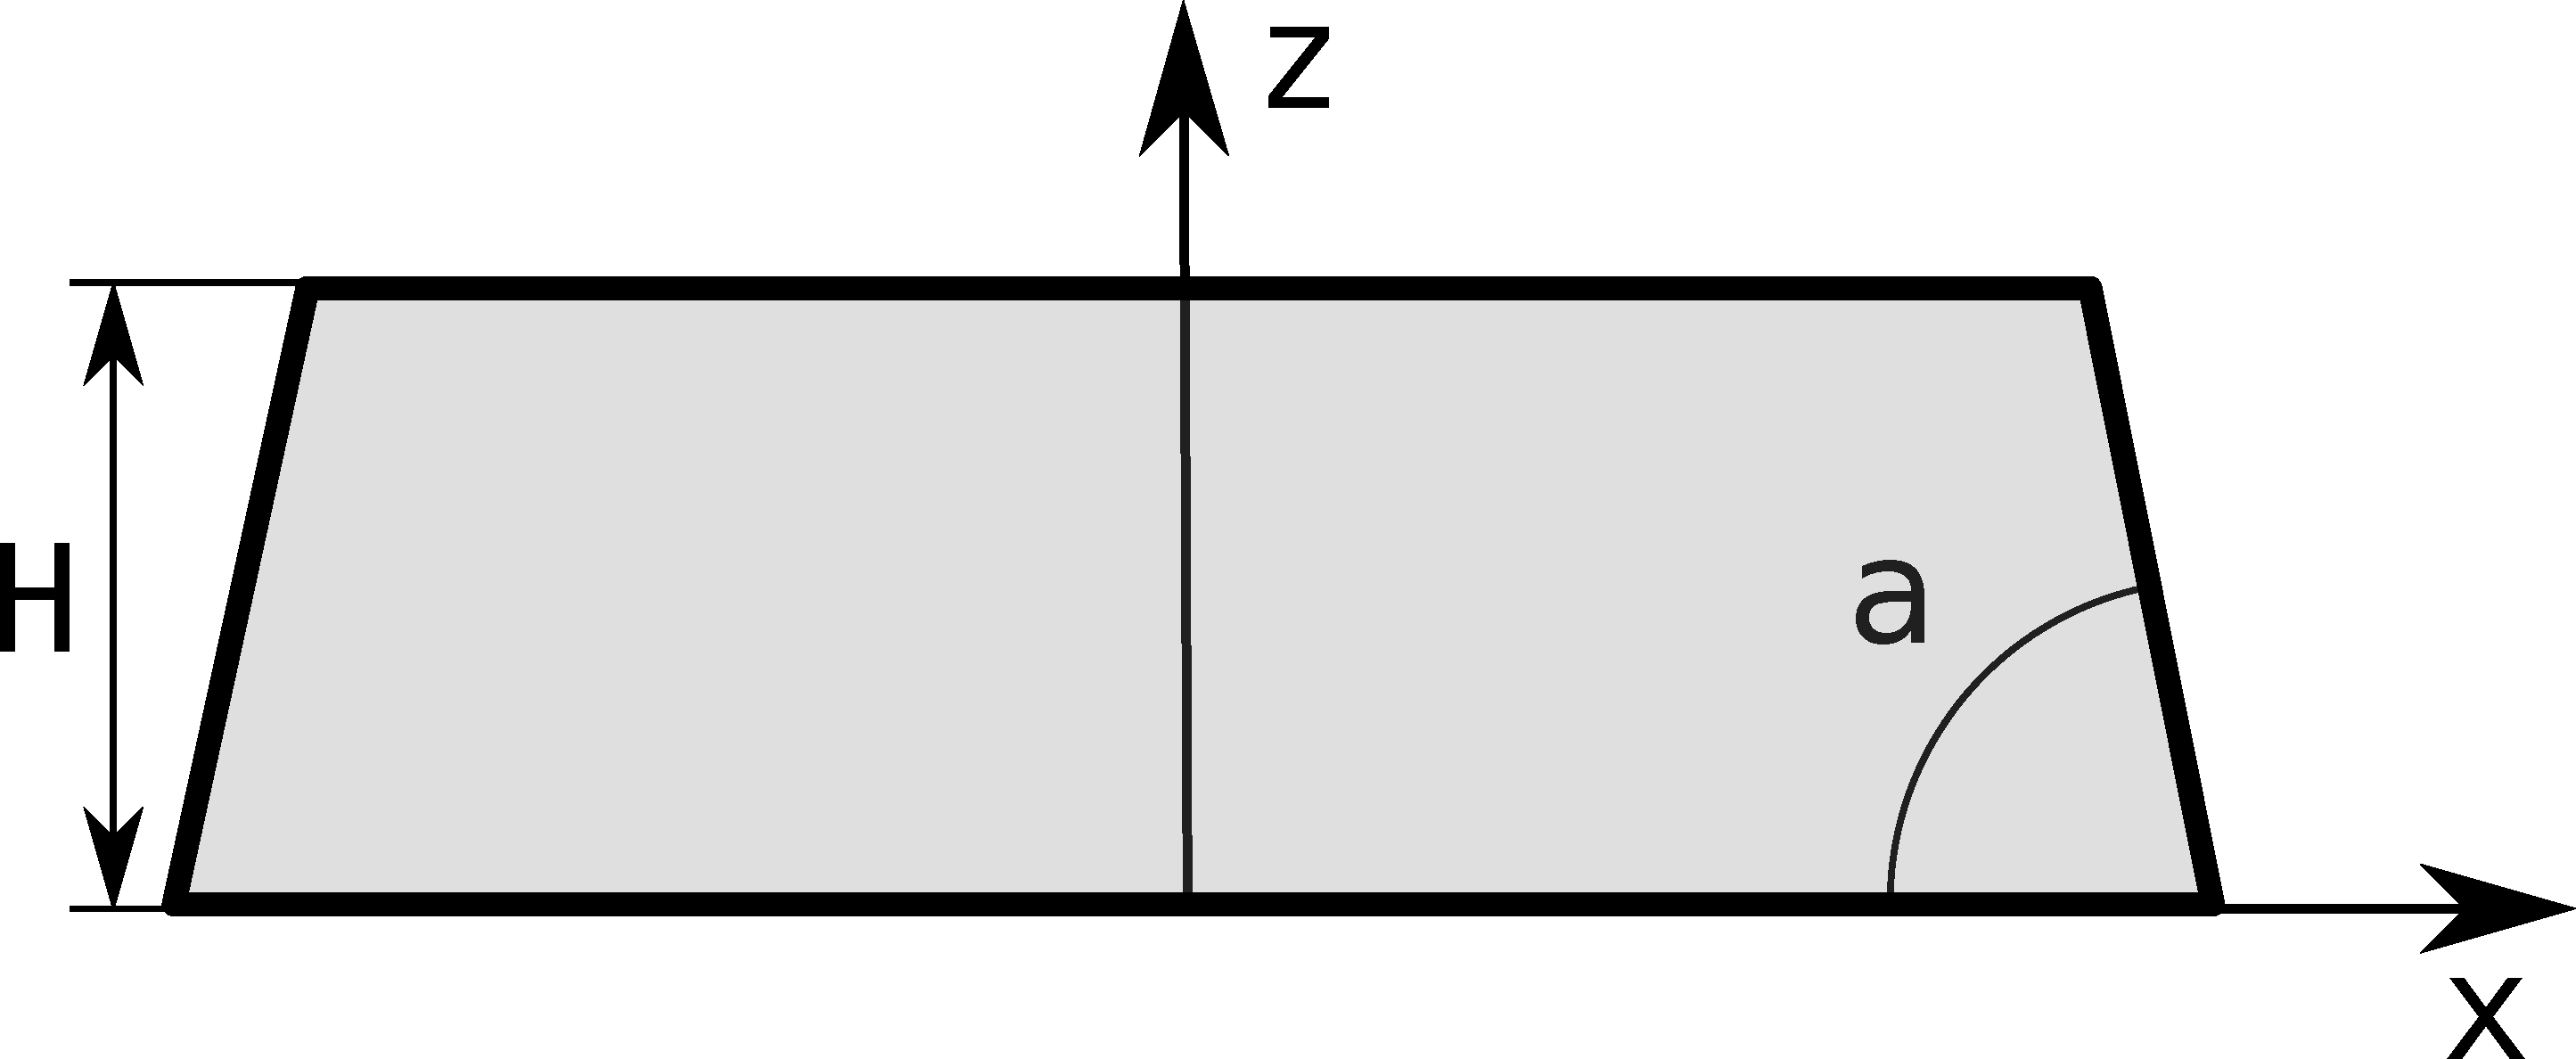
\includegraphics[width=.30\textwidth]{fig/cuts/AnisoPyramid2dxz.pdf}}}
\hfill
\caption{A truncated right pyramid with a rectangular base.}
\end{figure}

\FloatBarrier

\paragraph{Syntax and parameters}\strut\\[-2ex plus .2ex minus .2ex]
\begin{lstlisting}[language=python, style=eclipseboxed,numbers=none,nolol]
  FormFactorAnisoPyramid(length, width, height, alpha)
\end{lstlisting}
with the parameters
\begin{itemize}
\item \texttt{length} of the base, $L$,
\item \texttt{width} of the base, $W$,
\item \texttt{height}, $H$
\item \texttt{alpha}, angle between the base and a side face, $\alpha$.
\end{itemize}
They must fulfill
\begin{displaymath}
  H \le \frac{\tan\alpha}{2} L
  \quad\text{and}\quad
  H \le \frac{\tan\alpha}{2} W
\end{displaymath}

\paragraph{Form factor etc}\strut\\
Notation:
\begin{displaymath}
  \ell\coloneqq L/2,\quad
  w\coloneqq W/2,\quad
  h\coloneqq H/2,\quad
  f_\pm(z)\coloneqq \exp(\pm i z)\sinc(z).
\end{displaymath}
Results:
\begin{equation*}
\begin{array}{@{}l@{}l@{}}
\DS F=
\frac{H}{q_xq_y} \Big\{
   &+\DS  f_+\left(\left(\frac{q_x-q_y}{\tan\alpha} +q_z\right)h\right)
        \exp(-i(q_x\ell-q_y w))
\\[3.6ex]
   &\DS+ f_-\left(\left(\frac{q_x-q_y}{\tan\alpha} -q_z\right)h\right)
        \exp(+i(q_x\ell-q_y w))
\\[3.6ex]
   &\DS- f_+\left(\left(\frac{q_x+q_y}{\tan\alpha} +q_z\right)h\right)
        \exp(-i(q_x\ell+q_y w))
\\[3.6ex]
   &\DS- f_-\left(\left(\frac{q_x+q_y}{\tan\alpha} -q_z\right)h\right)
        \exp(+i(q_x\ell+q_y w))
\Big\},
\end{array}
\end{equation*}
\begin{equation*}
  V= H \Big[LW - \dfrac{(L + W)H}{\tan\alpha} + \dfrac{4}{3} \dfrac{H^2}{\tan^2\alpha}\Big].
\end{equation*}
\begin{equation*}
  S=LW.
\end{equation*}

\paragraph{Example}\strut\\
Figure~\ref{fig:FFAnisoPyramidEx} shows the normalized intensity
$|F|^2/V^2$, computed with $L=20$~nm, $W=16$~nm, $H=13$~nm, and
$\alpha=60^{\circ}$.

\begin{figure}[H]
\begin{center}
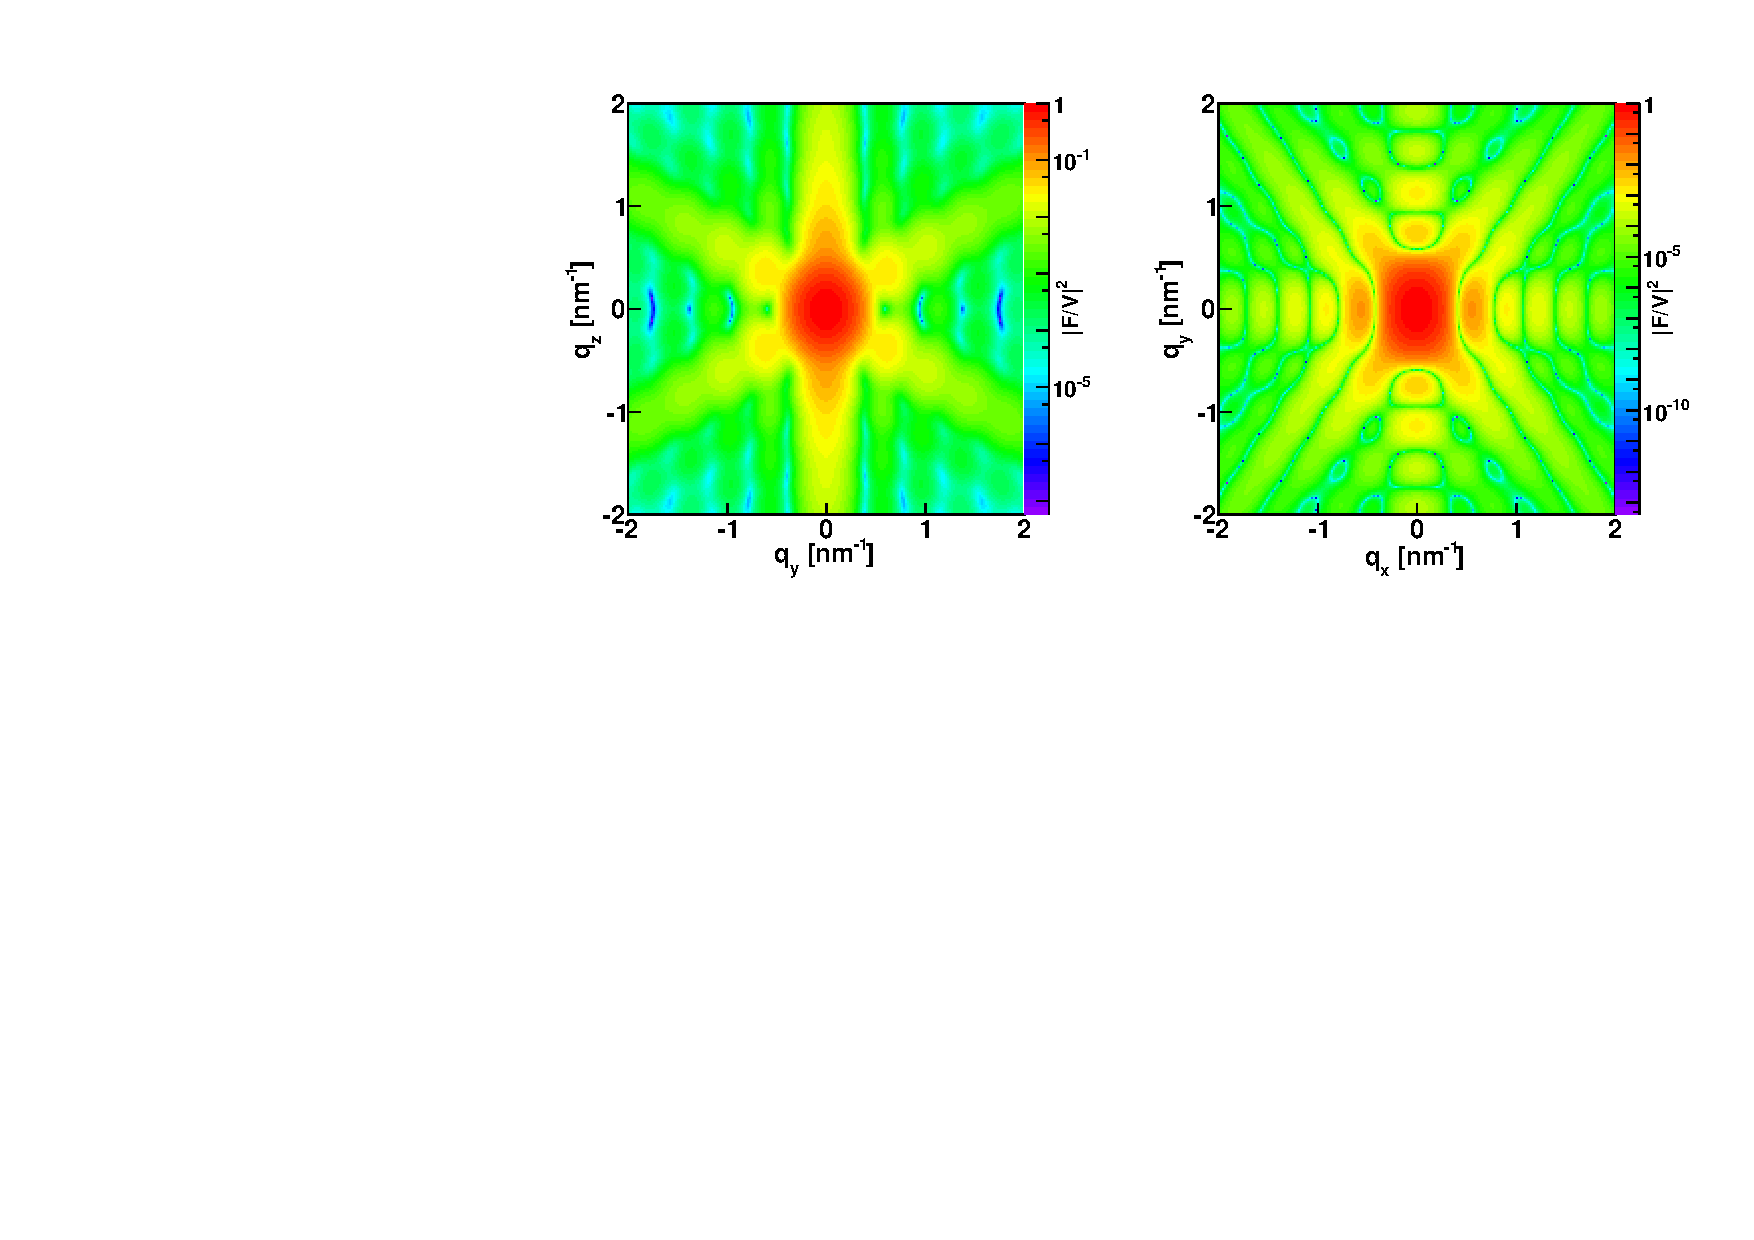
\includegraphics[angle=-90,width=\textwidth]{fig/ff/figffanisopyramid.pdf}
\end{center}
\caption{Normalized intensity for the form factor of an anisotropic
  pyramid $|F|^2/V^2$, plotted against ($q_y$, $q_z$) and  ($q_x$, $q_y$) and computed with \Code{FormFactorAnisoPyramid(20.*nanometer, 16.*nanometer, 13.*nanometer, 60.*degree)}.}
\label{fig:FFAnisoPyramidEx}
\end{figure}

\paragraph{References}\strut\\
Agrees with the \E{In-plane anisotropic pyramid} form factor of \IsGISAXS\
\cite[Eq.~2.40]{Laz08} \cite[Eq.~217]{ReLL09},
except for different parametrization and
for a refactoring of the analytical expression for $F(\q)$.

%-------------------------------------------------------------------------------
\FloatBarrier\newpage
\subsection{Box (cuboid)} \label{sec:Box}
  \index{Box (form factor)}
  \index{Cuboid (form factor)}
  \index{Prism (form factor)!reactangular (Box)}
  \index{FormFactorBox@\Code{FormFactorBox}}
%-------------------------------------------------------------------------------

\paragraph{Real-space geometry}\strut\\

\begin{figure}[H]
\hfill
\subfigure[Perspective]{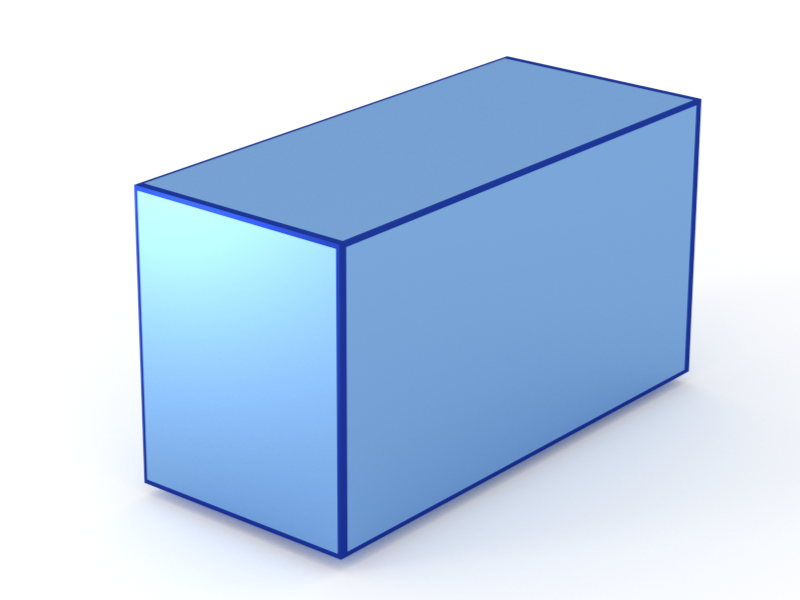
\includegraphics[width=.24\textwidth]{fig/blue/Box3d.png}}
\hfill
\subfigure[Top view]{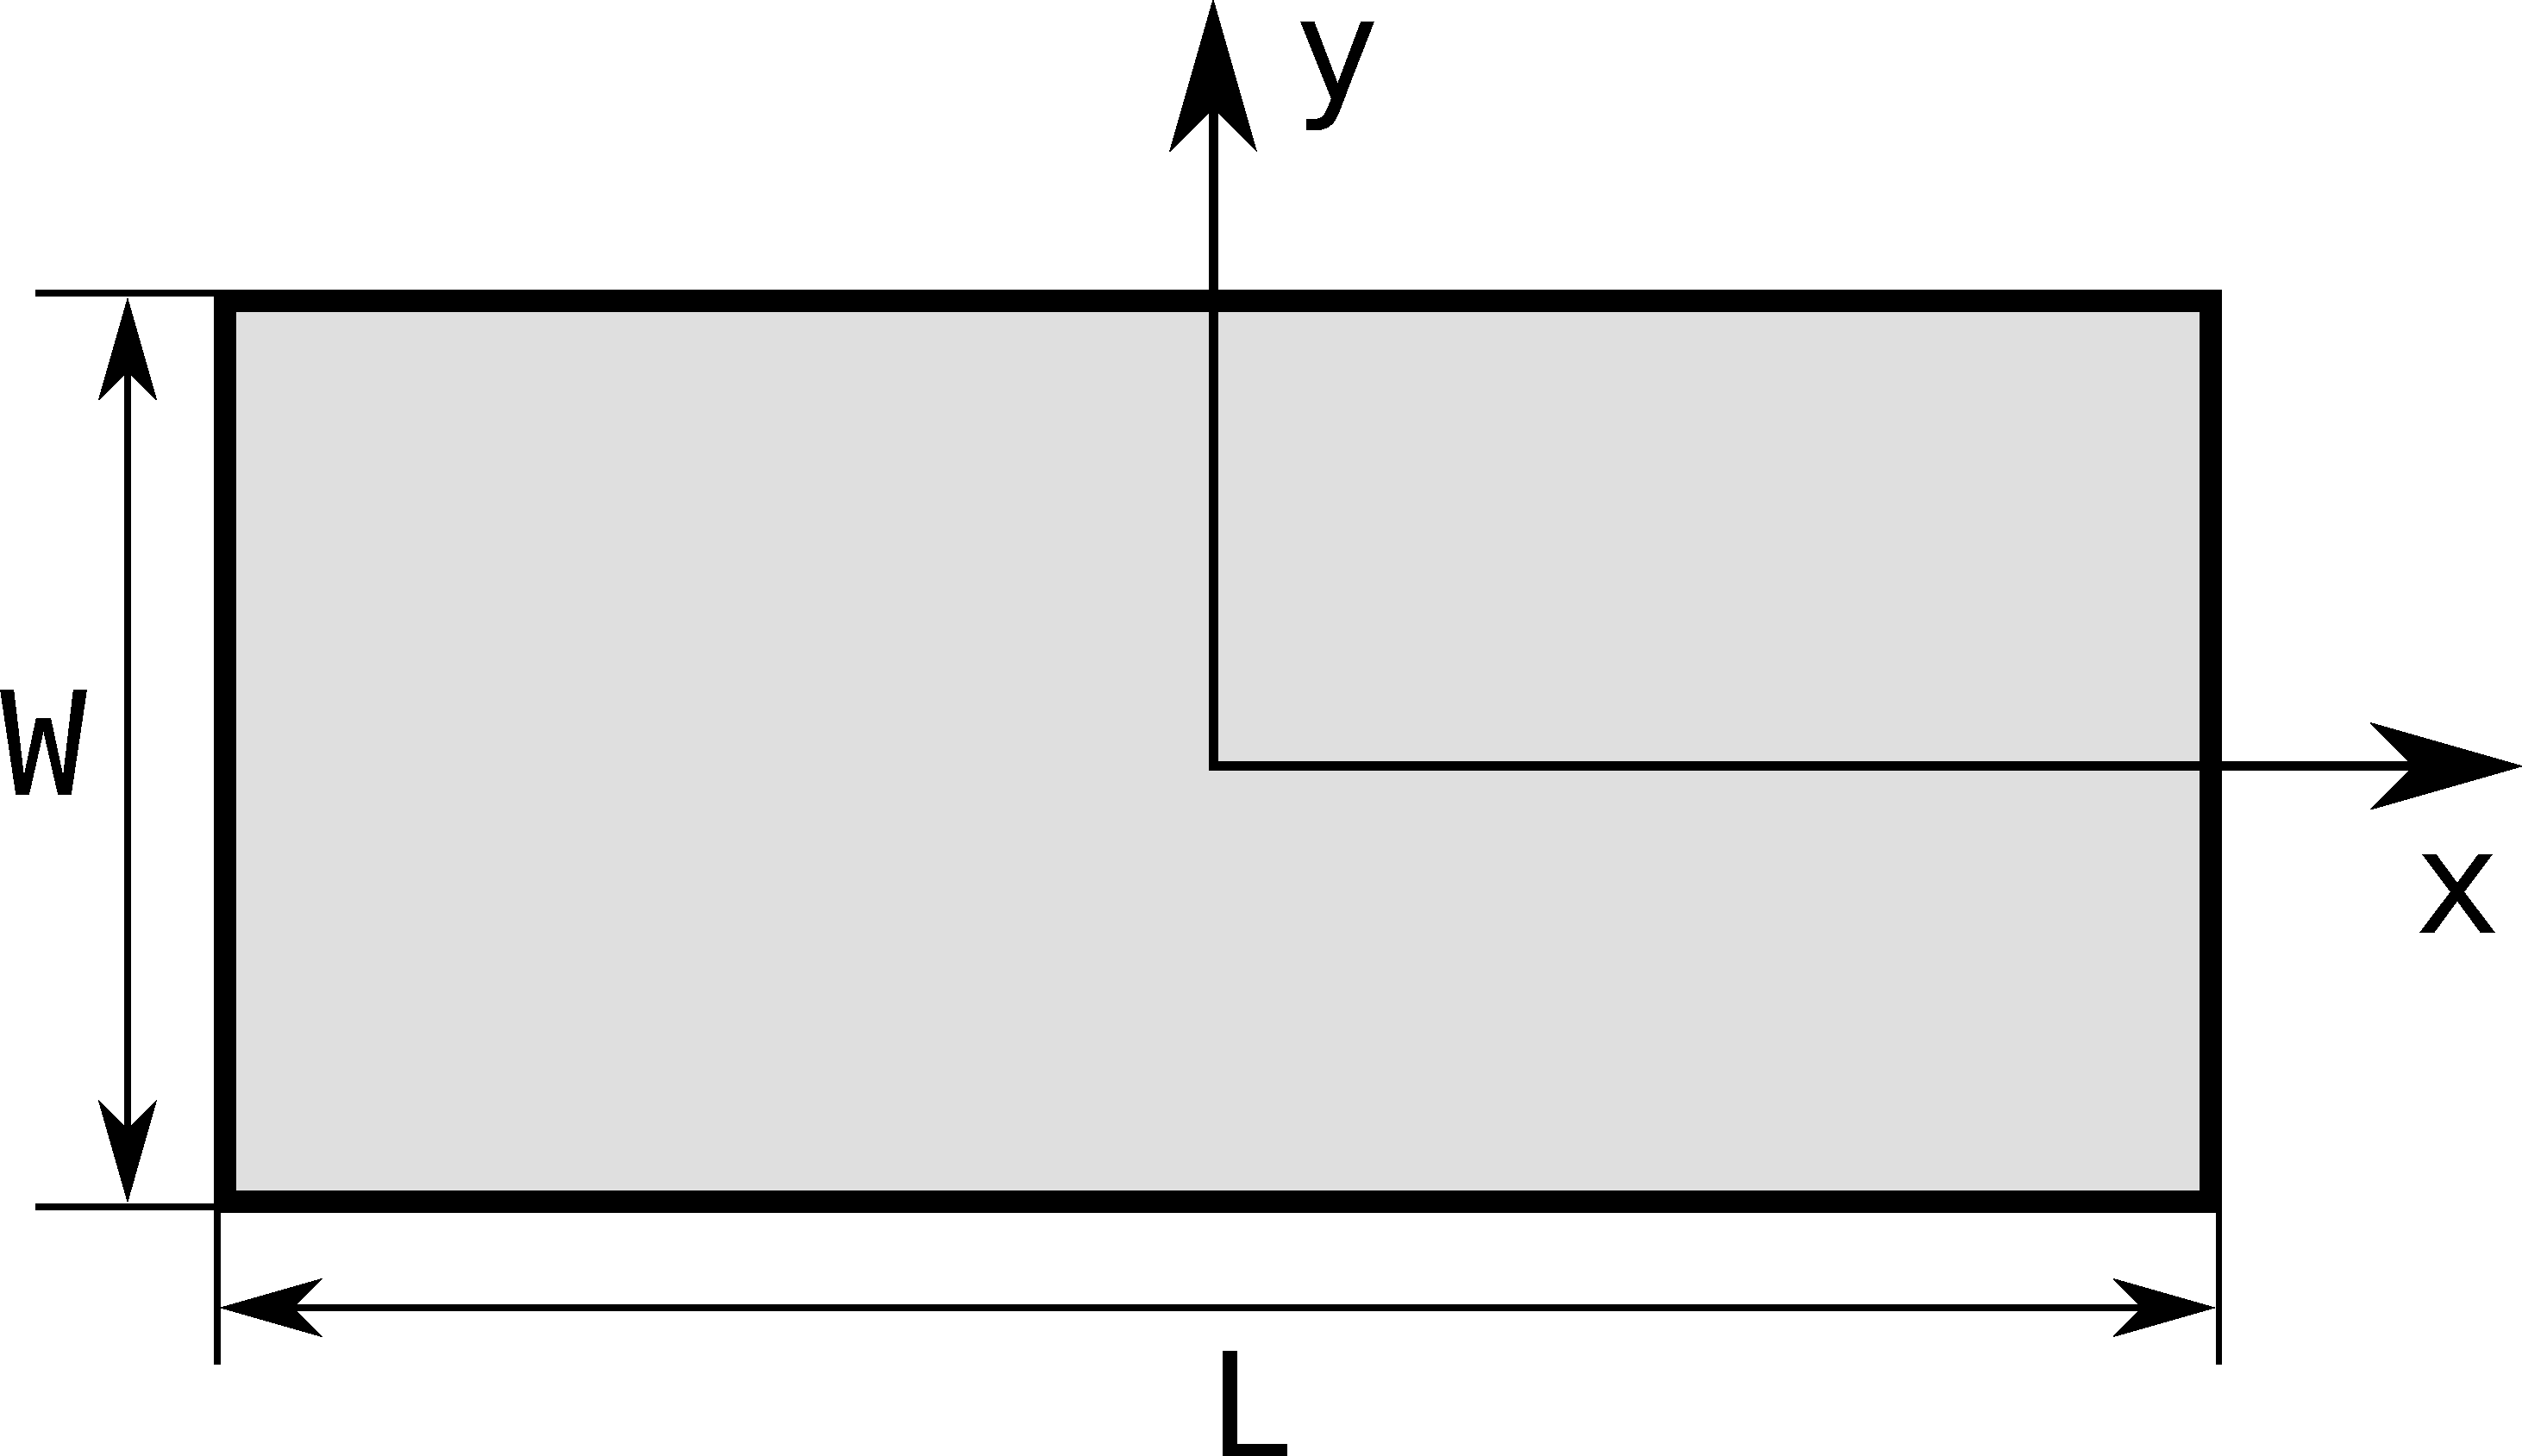
\includegraphics[width=.30\textwidth]{fig/cuts/Box2dxy.pdf}}
\hfill
\subfigure[Side view]{\raisebox{2mm}{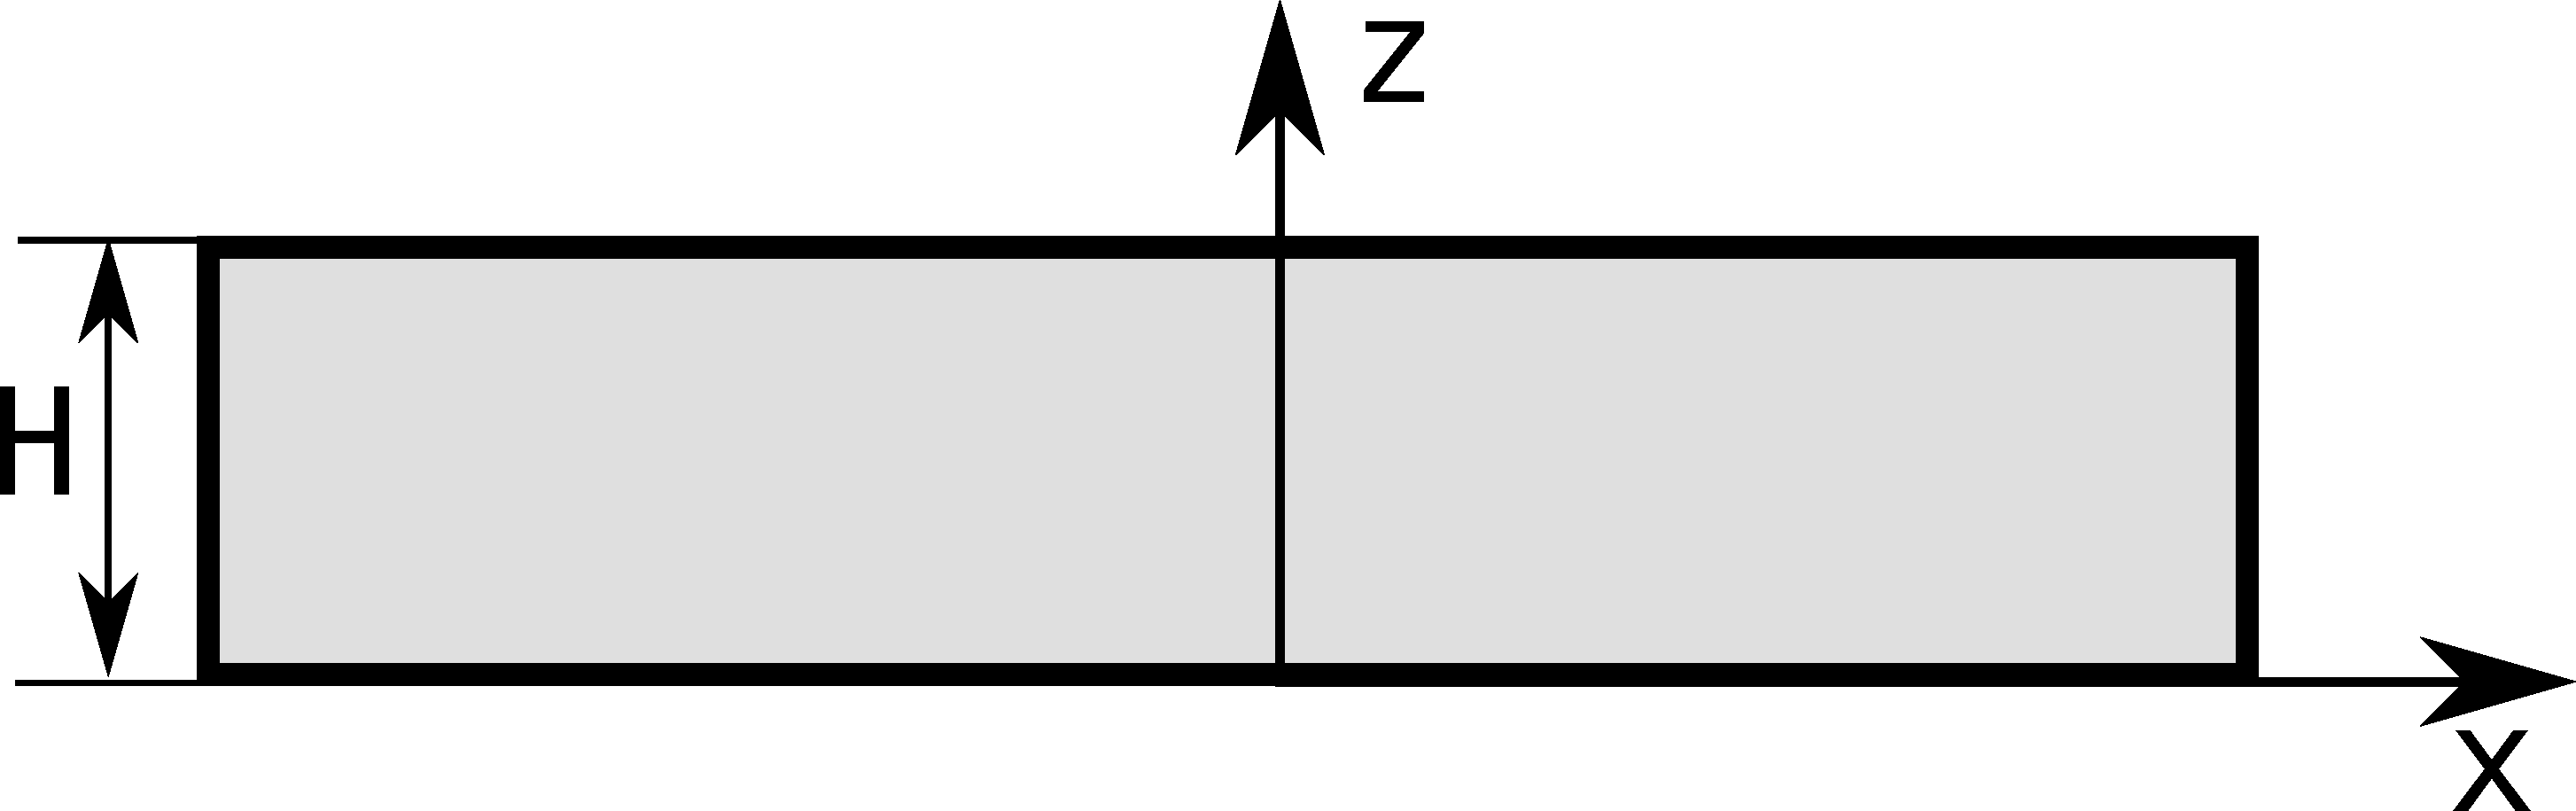
\includegraphics[width=.30\textwidth]{fig/cuts/Box2dxz.pdf}}}
\hfill
\caption{A rectangular cuboid.}
\end{figure}

\FloatBarrier

\paragraph{Syntax and parameters}\strut\\[-2ex plus .2ex minus .2ex]
\begin{lstlisting}[language=python, style=eclipseboxed,numbers=none,nolol]
  FormFactorBox(length, width, height)
\end{lstlisting}
with the parameters
\begin{itemize}
\item \texttt{length} of the base, $L$,
\item \texttt{width} of the base, $W$,
\item \texttt{height}, $H$.
\end{itemize}


\paragraph{Form factor etc}

\begin{equation*}
F= L W H\exp\left(i q_z \frac{H}{2}\right) \sinc\left(q_x \frac{L}{2}\right)
\sinc\left(q_y \frac{W}{2}\right) \sinc\left(q_z \frac{H}{2}\right),
\end{equation*}
\begin{equation*}
  V= LWH,
\end{equation*}
\begin{equation*}
  S = LW.
\end{equation*}

\paragraph{Example}\strut\\
Figure~\ref{fig:FFBoxEx} shows the normalized intensity
$|F|^2/V^2$, computed with $L=20$~nm, $W=16$~nm, and $H=13$~nm:

\begin{figure}[H]
\begin{center}
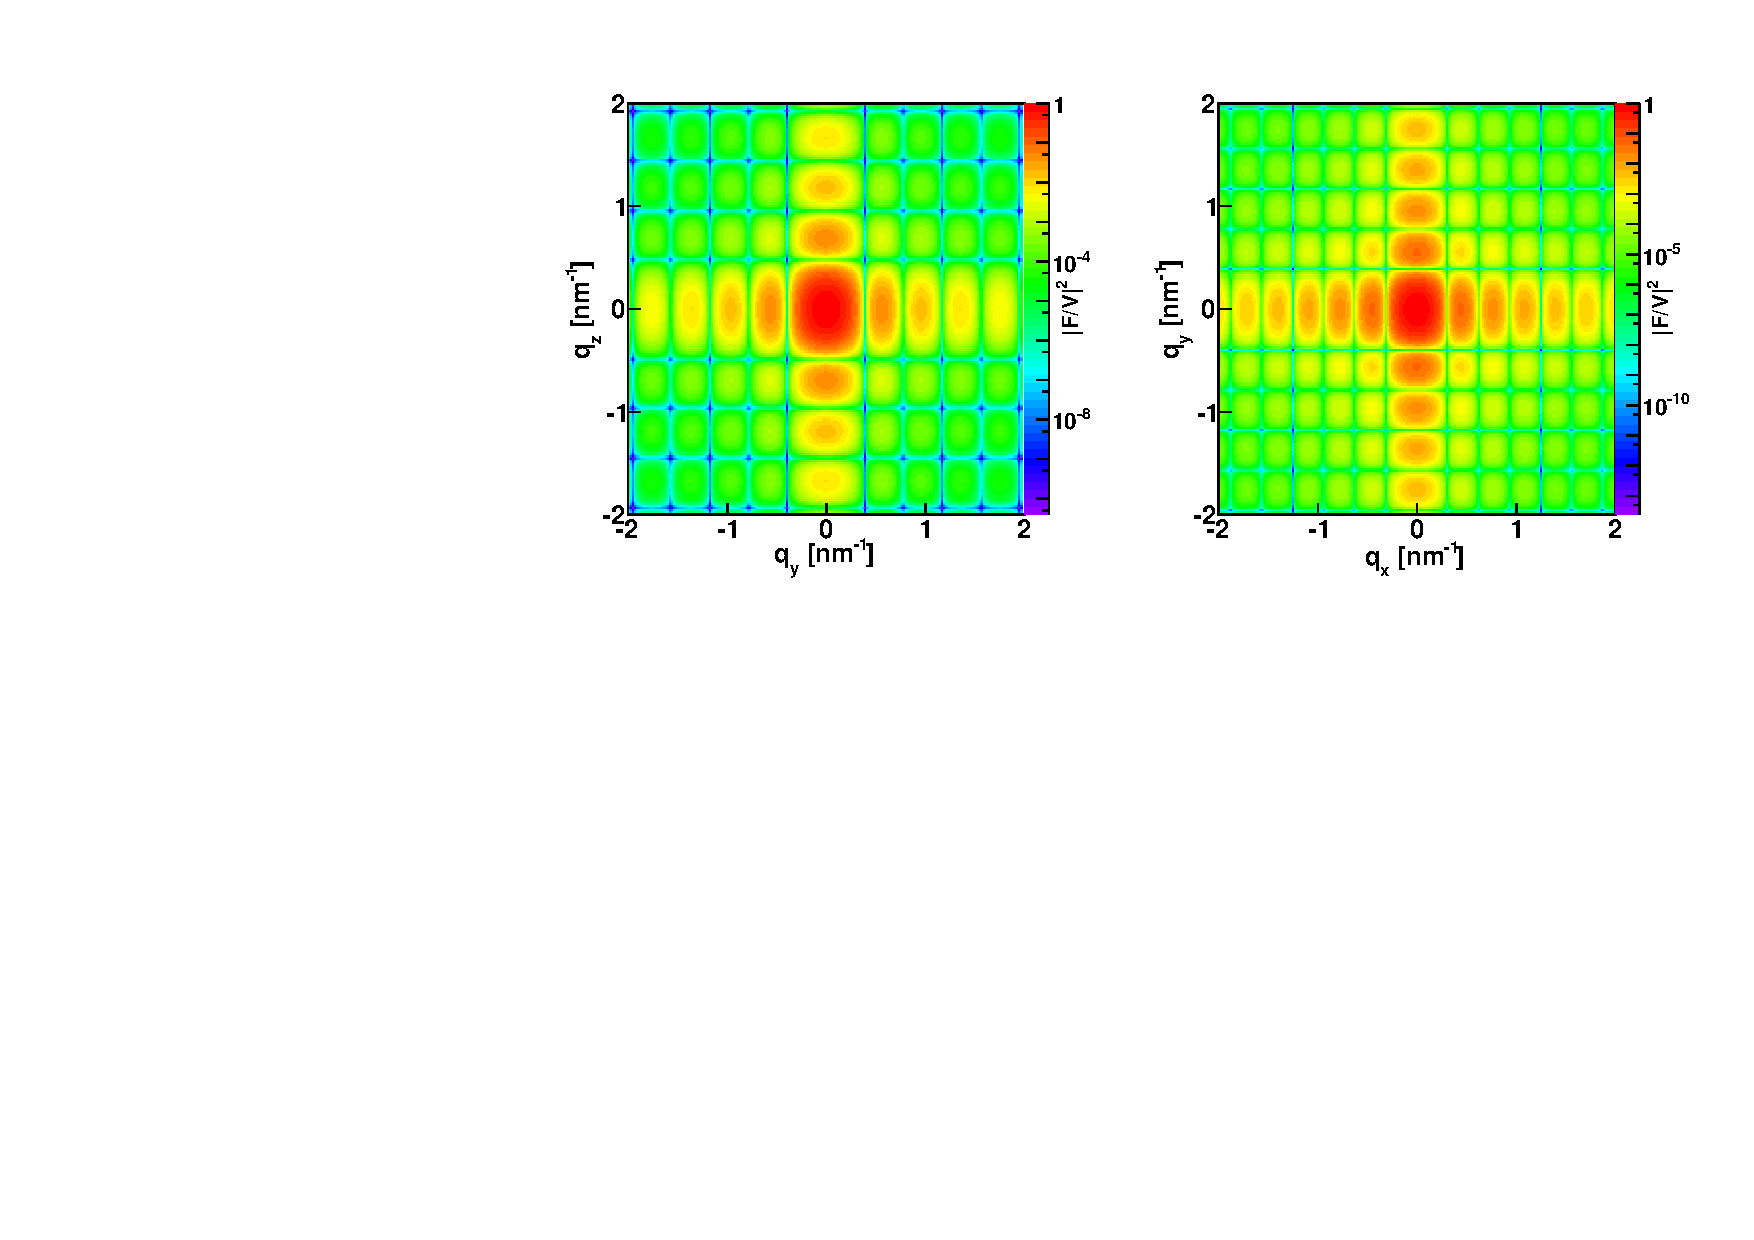
\includegraphics[angle=-90,width=\textwidth]{fig/ff/figffbox.pdf}
\end{center}
\caption{Normalized intensity for the form factor of a Box plotted against ($q_y$, $q_z$) and  ($q_x$, $q_y$) and computed with \Code{FormFactorBox(20.*nanometer, 16.*nanometer, 13.*nanometer)}.}
\label{fig:FFBoxEx}
\end{figure}

\paragraph{References}\strut\\
Agrees with \E{Box} form factor of \IsGISAXS\
\cite[Eq.~2.38]{Laz08} \cite[Eq.~214]{ReLL09},
except for factors $1/2$ in the definitions of parameters $L$, $W$, $H$.

%-------------------------------------------------------------------------------
\clearpage
\subsection{Cone (circular)} \label{sec:Cone} 
  \index{Cone (form factor)!circular}
  \index{Truncated cone (form factor)}
  \index{FormFactorCone@\Code{FormFactorCone}}
%-------------------------------------------------------------------------------

\paragraph{Real-space geometry}

\begin{figure}[H]
\hfill
\subfigure[Perspective]{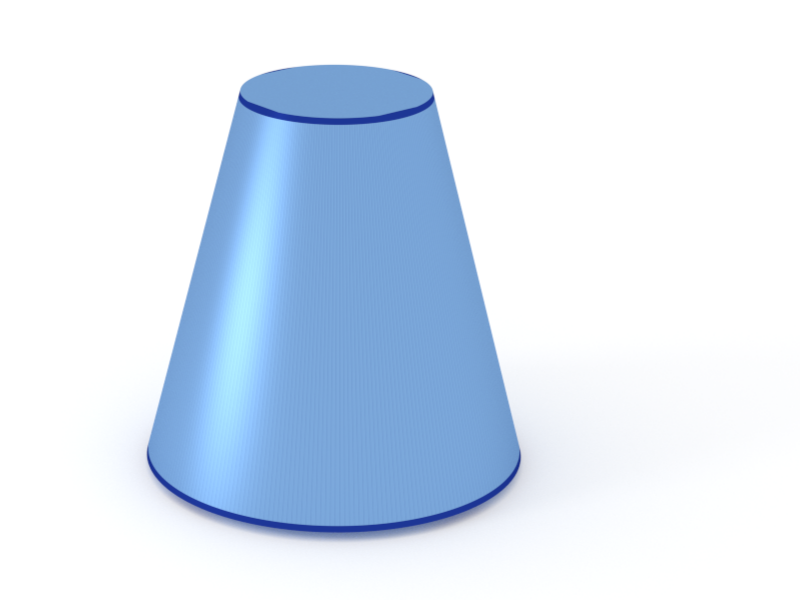
\includegraphics[width=.24\textwidth]{fig/blue/Cone3d.png}}
\hfill
\subfigure[Top view]{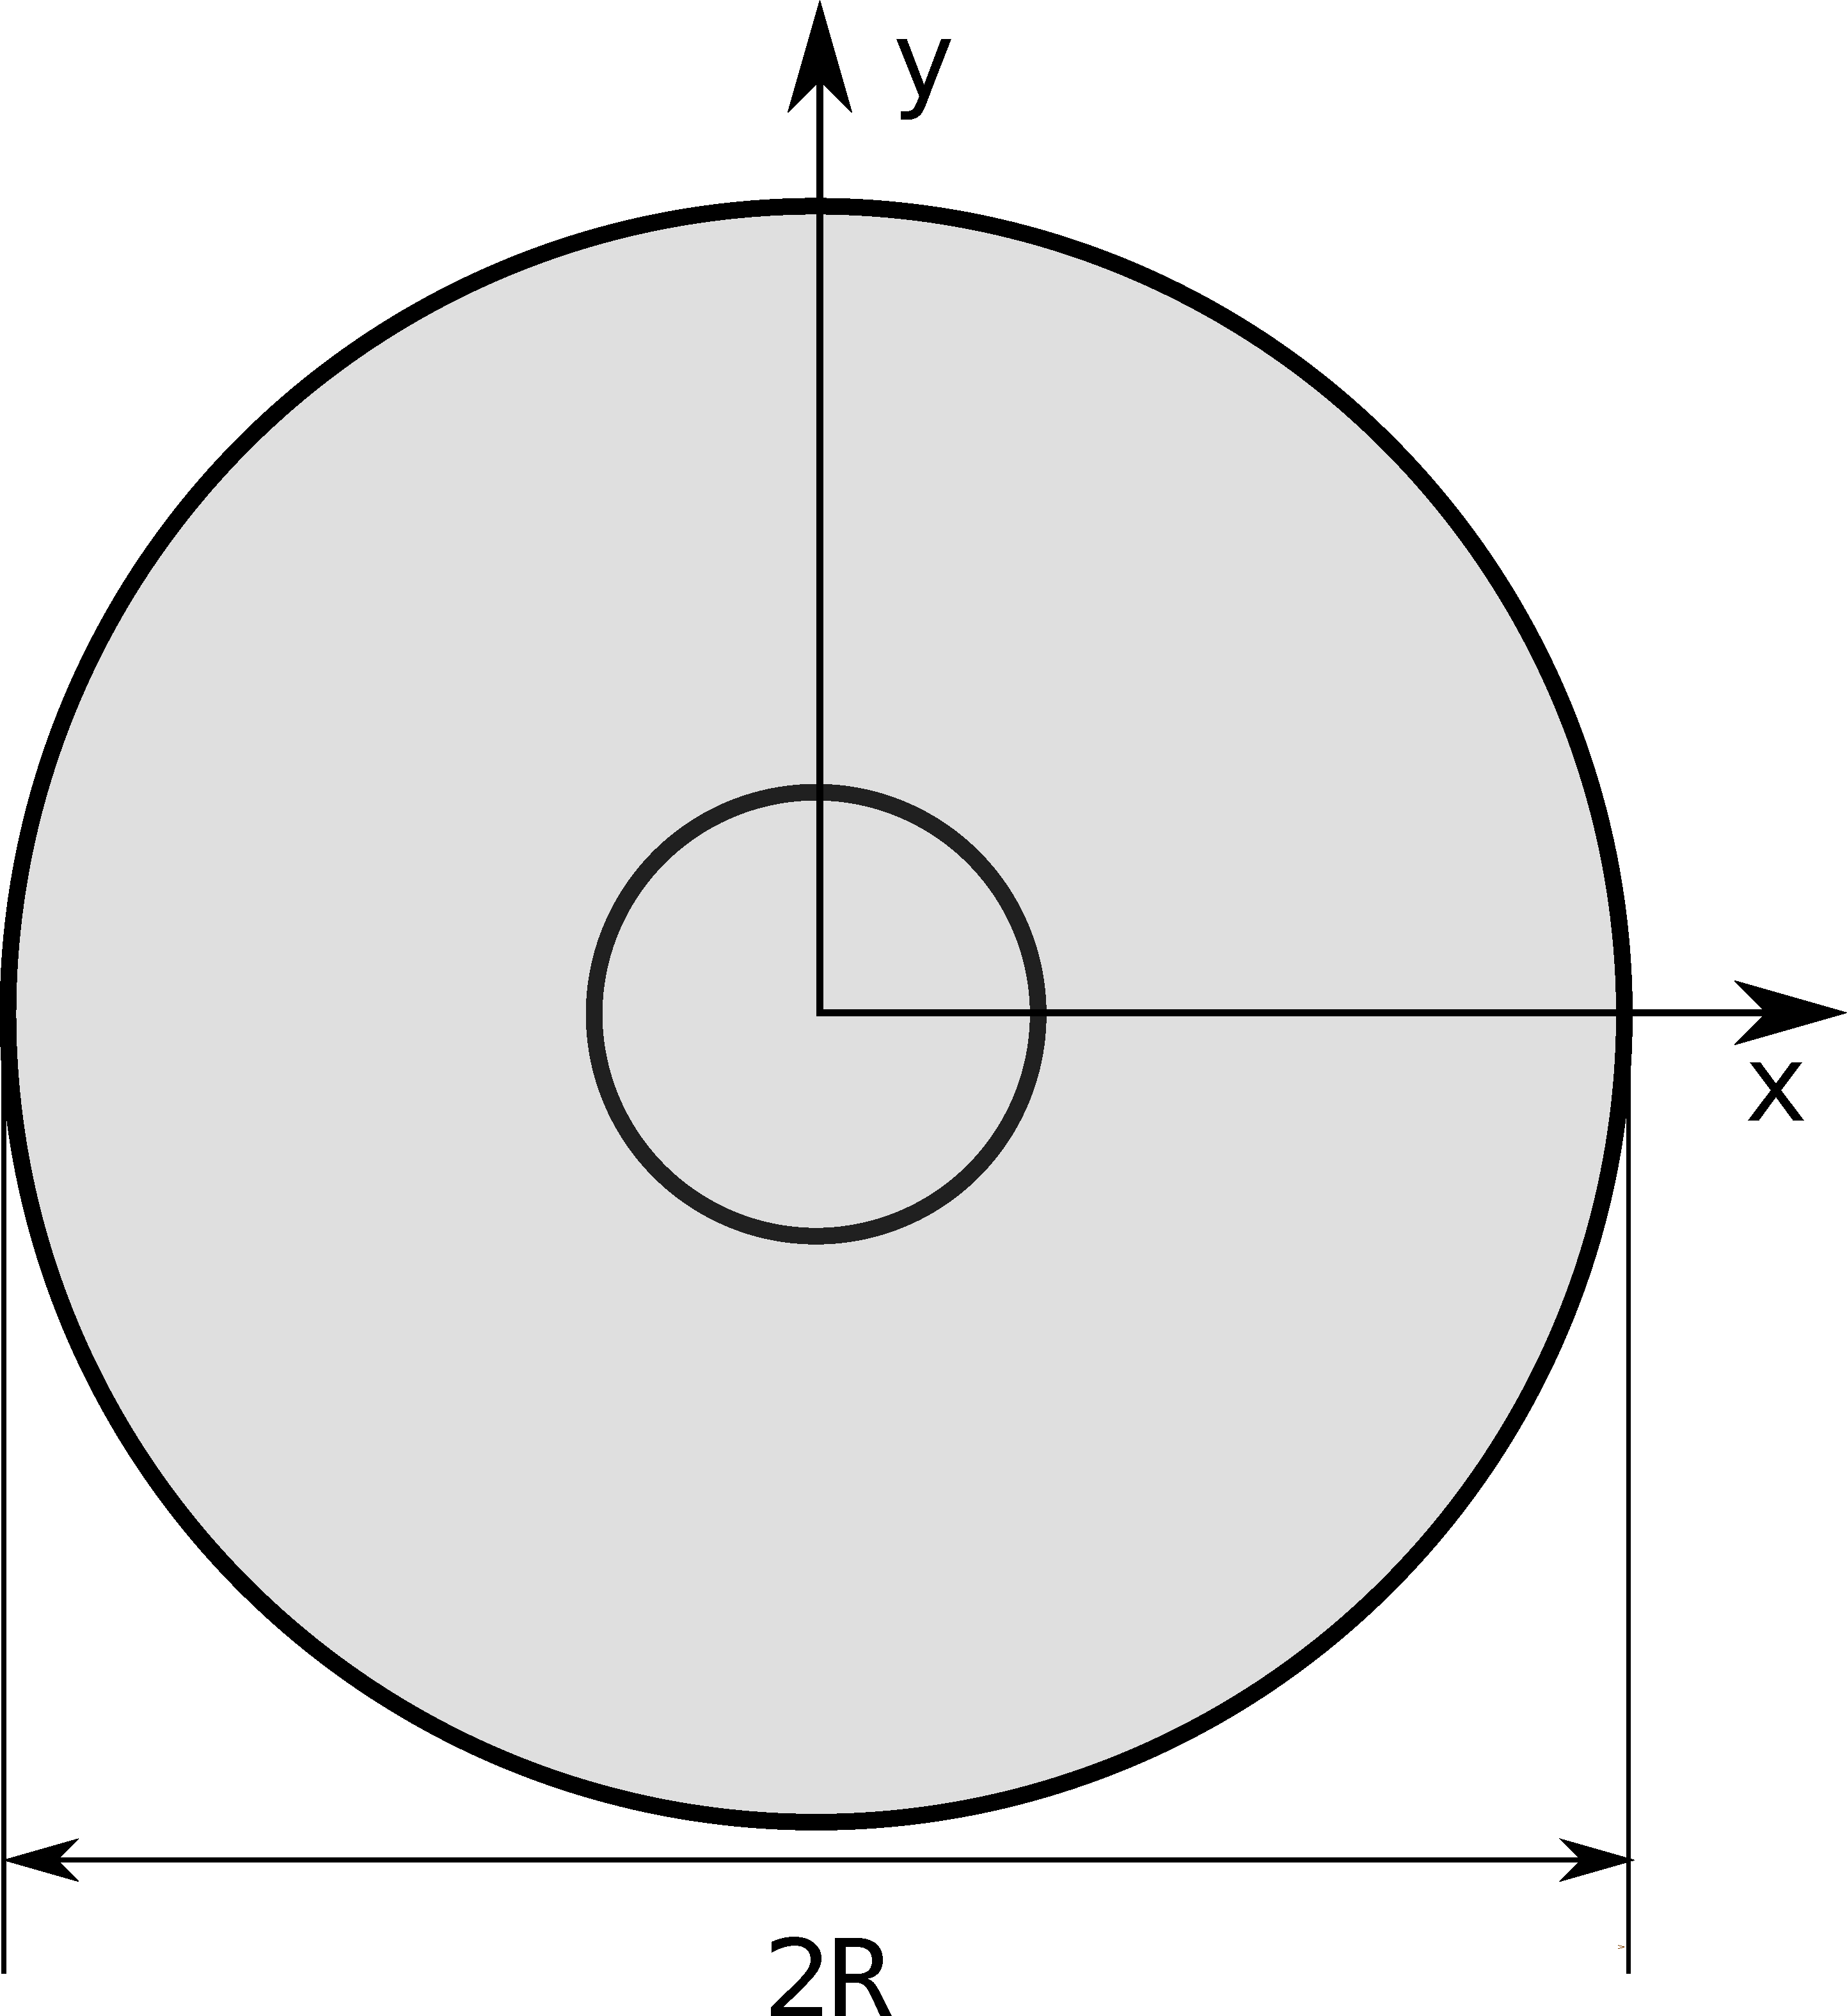
\includegraphics[width=.30\textwidth]{fig/cuts/Cone2dxy.pdf}}
\hfill
\subfigure[Side view]{\raisebox{3mm}{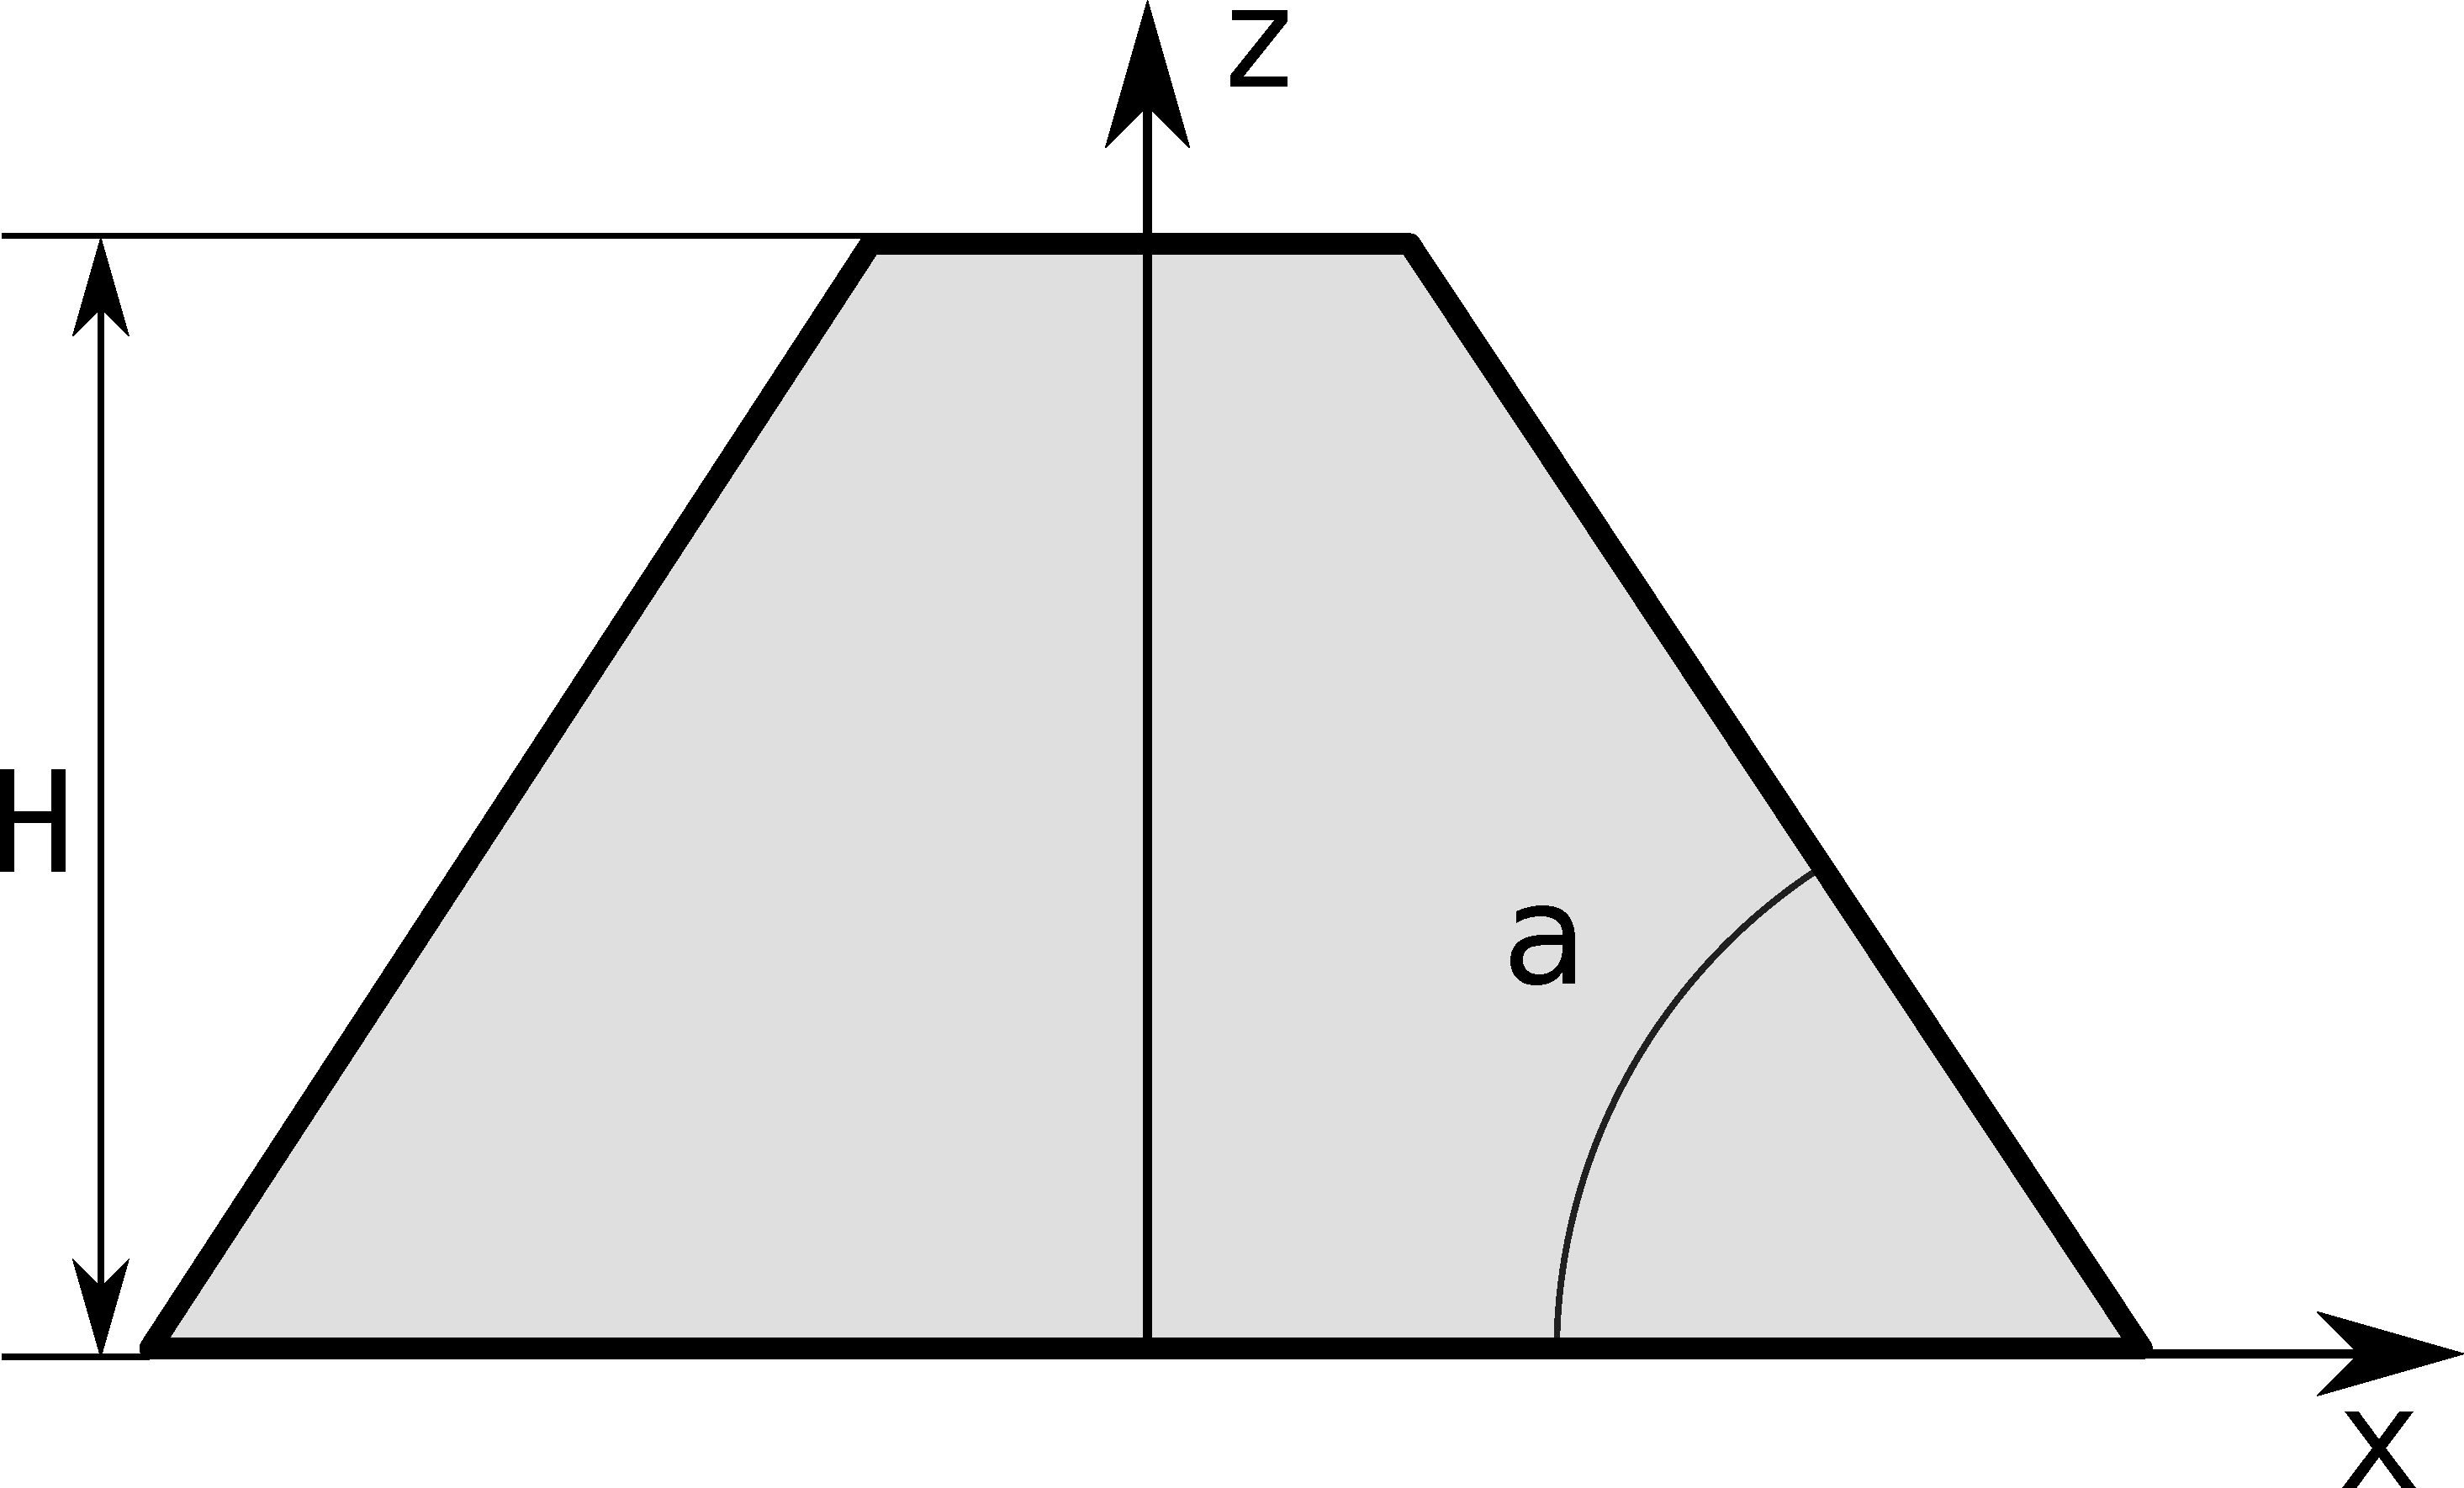
\includegraphics[width=.30\textwidth]{fig/cuts/Cone2dxz.pdf}}}
\hfill
\caption{A truncated cone with circular base.}
\end{figure}

\paragraph{Syntax and parameters}\strut\\[-2ex plus .2ex minus .2ex]
\begin{lstlisting}[language=python, style=eclipseboxed,numbers=none,nolol]
  FormFactorCone(radius, height, alpha)
\end{lstlisting}
with the parameters
\begin{itemize}
\item \texttt{radius}, $R$,
\item \texttt{height}, $H$,
\item \texttt{alpha}, angle between the side and the base, $\alpha$.
\end{itemize}
They must fulfill
\begin{displaymath}
  H\le R\tan\alpha.
\end{displaymath}


\paragraph{Form factor etc}\strut\\
Notation:
\begin{equation*}
  R_H \coloneqq R-\dfrac{H}{\tan \alpha}, \quad
  q_{\parallel} \coloneqq \sqrt{q_x^2+ q_y^2}, \quad
  \tilde{q}_z \coloneqq q_z \tan\alpha.
\end{equation*}
Results:
\begin{equation*}
  F = 2\pi \tan\alpha\; \e^{i\tilde{q}_z R}
      \int_{R_H}^R \!\d\rho\, \rho^2
        \frac{J_1(q_{\parallel}\rho)}{q_{\parallel}\rho}\,\e^{-i\tilde{q}_z \rho},
\end{equation*}
\begin{equation*}
  V = \dfrac{\pi}{3}\tan\alpha  \left( R^3 - R_H^3\right),
\end{equation*}
\begin{equation*}
  S=\pi R^2.
\end{equation*}

\paragraph{Example}\strut\\
Figure~\ref{fig:FFConeEx} shows the normalized intensity
$|F|^2/V^2$, computed with $R=10$~nm, $H=13$~nm, and $\alpha=60^{\circ}$.
\begin{figure}[H]
\begin{center}
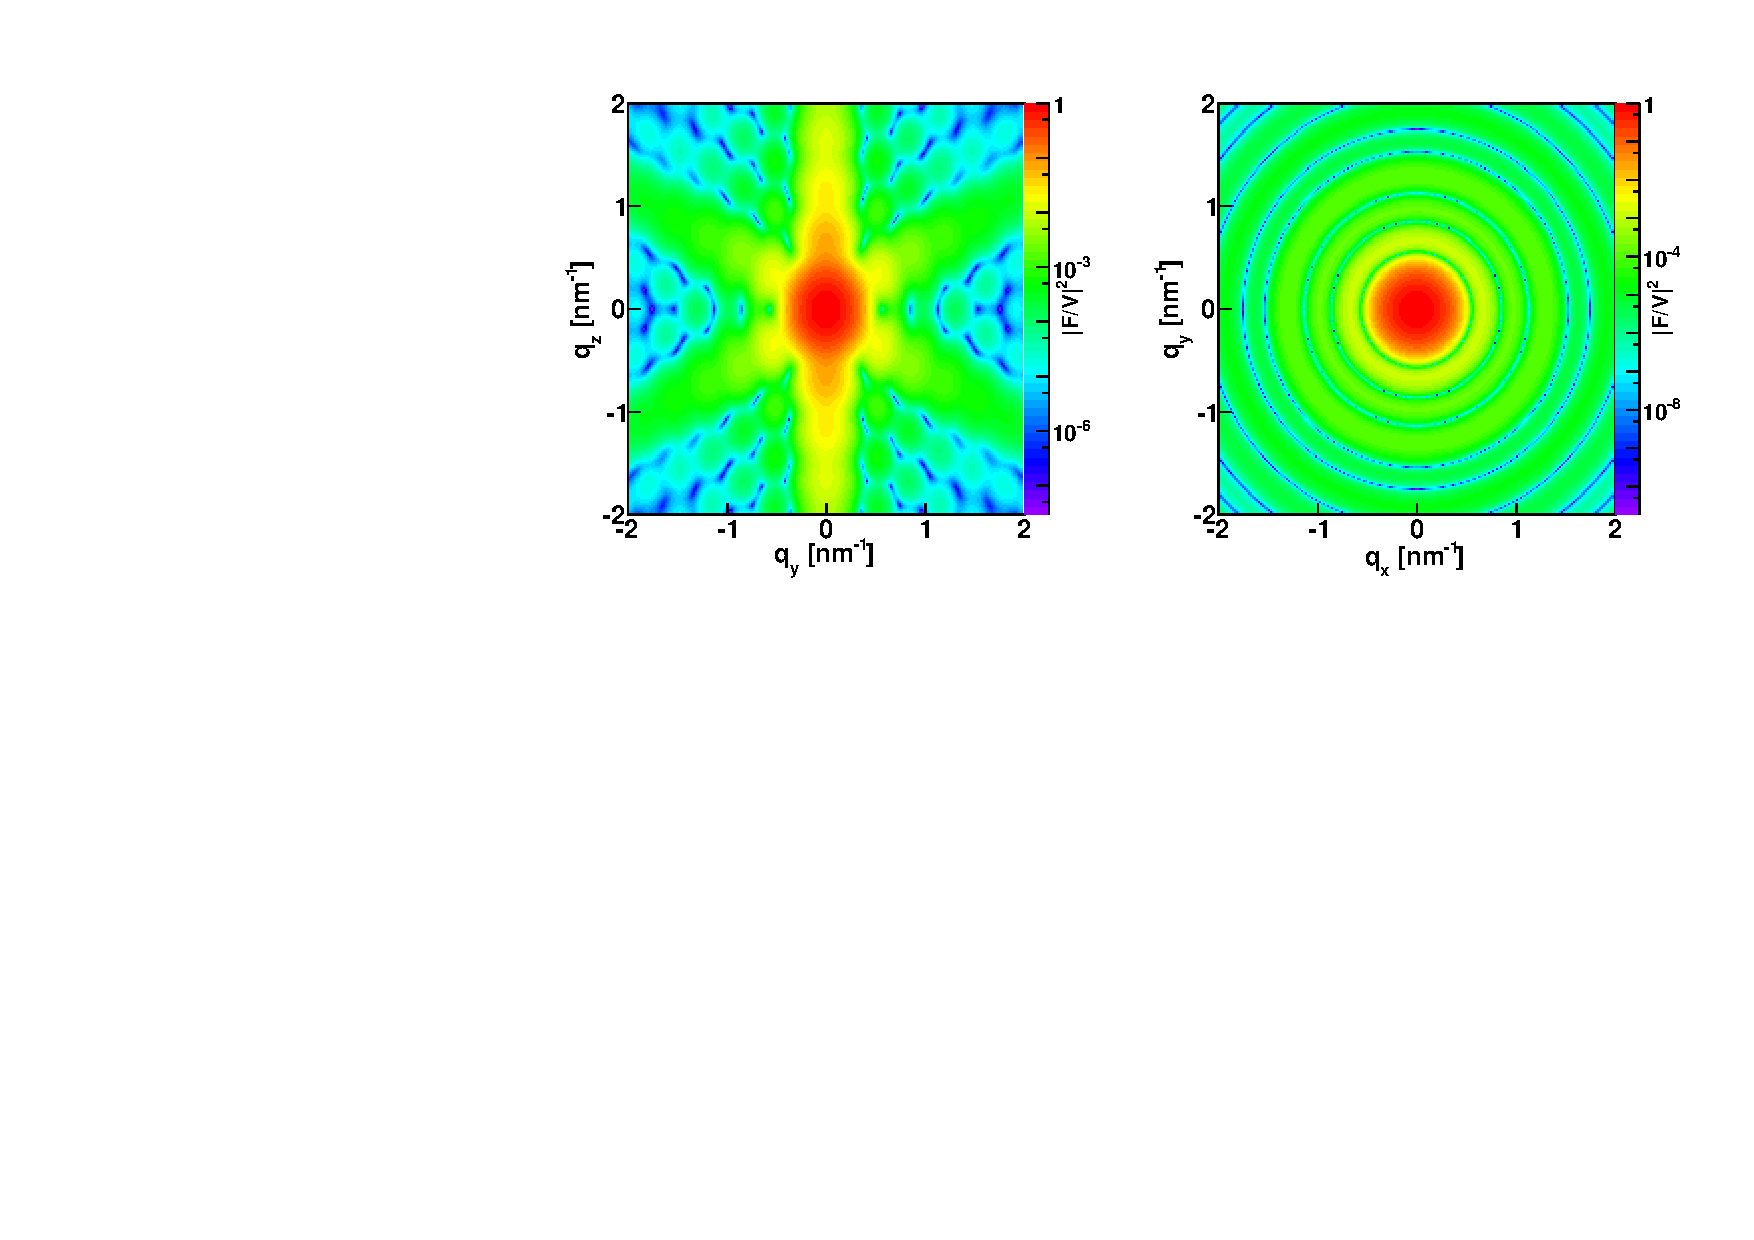
\includegraphics[angle=-90,width=\textwidth]{fig/ff/figffcone.pdf}
\end{center}
\caption{Normalized intensity for the form factor of a Cone plotted against ($q_y$, $q_z$) and ($q_x$, $q_y$.) It
  has been  computed with \Code{FormFactorCone(10.*nanometer,13.*nanometer, 60.*degree)}.}
\label{fig:FFConeEx}
\end{figure}

\paragraph{References}\strut\\
Agrees with \E{Cone} form factor of \IsGISAXS\
\cite[Eq.~2.28]{Laz08} \cite[Eq.~225]{ReLL09},
except for a substitution $z\to\rho$ in our expression for~$F$.


%-------------------------------------------------------------------------------
\clearpage
\subsection{Cone6 (hexagonal)} \label{sec:Cone6}
  \index{Cone (form factor)!hexagonal (Cone6)}
  \index{Pyramid (form factor)!hexagonal (Cone6)}
  \index{Truncated pyramid (form factor)!hexagonal (Cone6)}
  \index{FormFactorCone6@\Code{FormFactorCone6}}
%-------------------------------------------------------------------------------

\paragraph{Real-space geometry}\strut\\

\begin{figure}[H]
\hfill
\subfigure[Perspective]{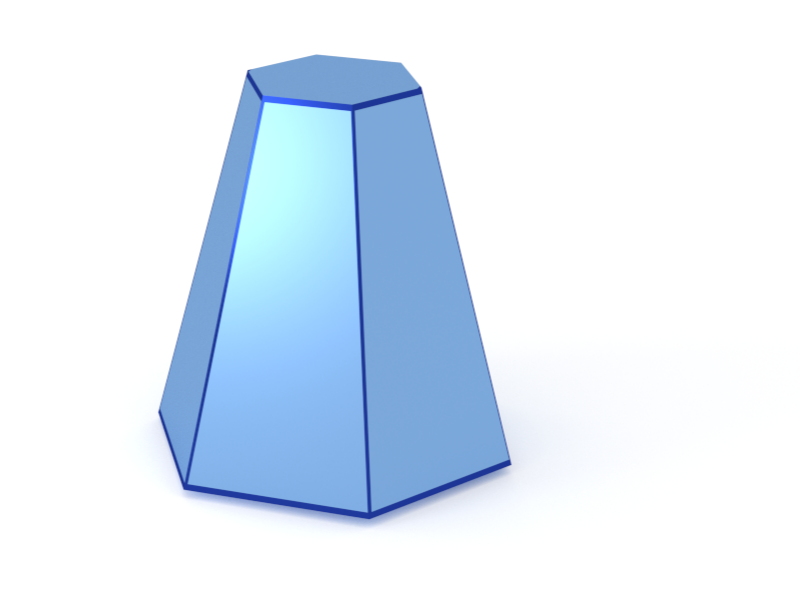
\includegraphics[width=.24\textwidth]{fig/blue/Cone63d.png}}
\hfill
\subfigure[Top view]{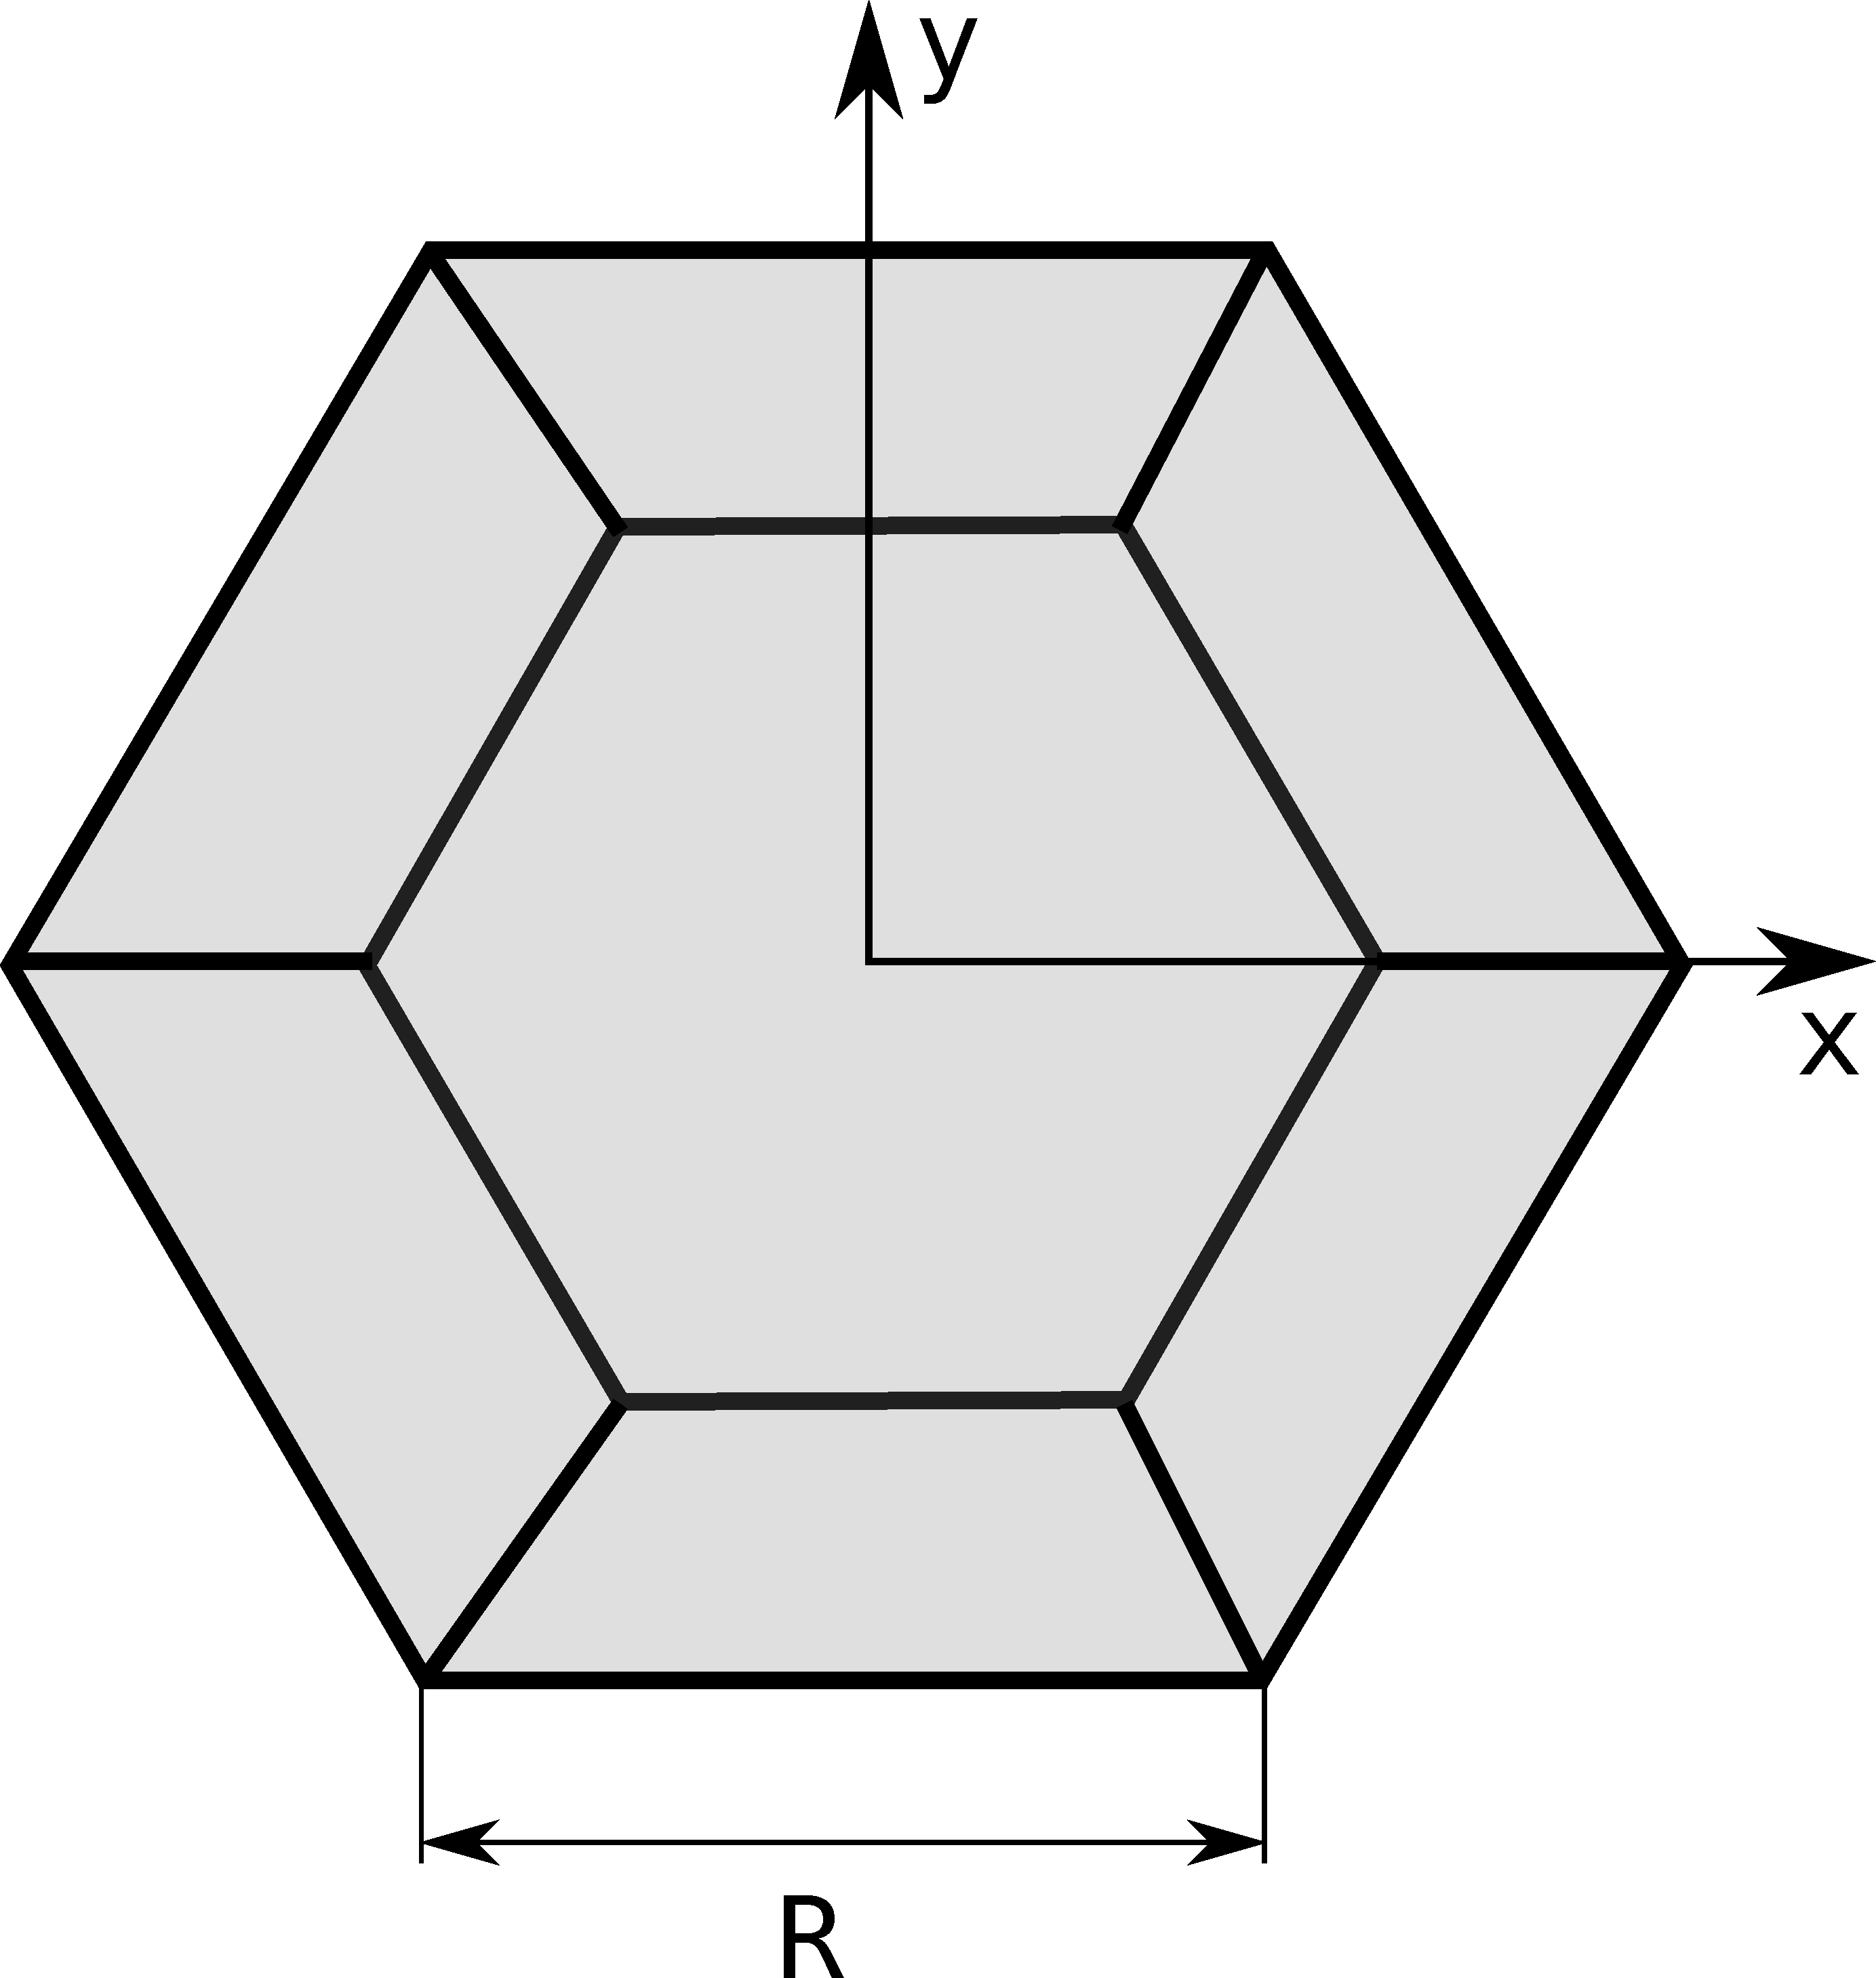
\includegraphics[width=.30\textwidth]{fig/cuts/Cone62dxy.pdf}}
\hfill
\subfigure[Side view]{\raisebox{5mm}{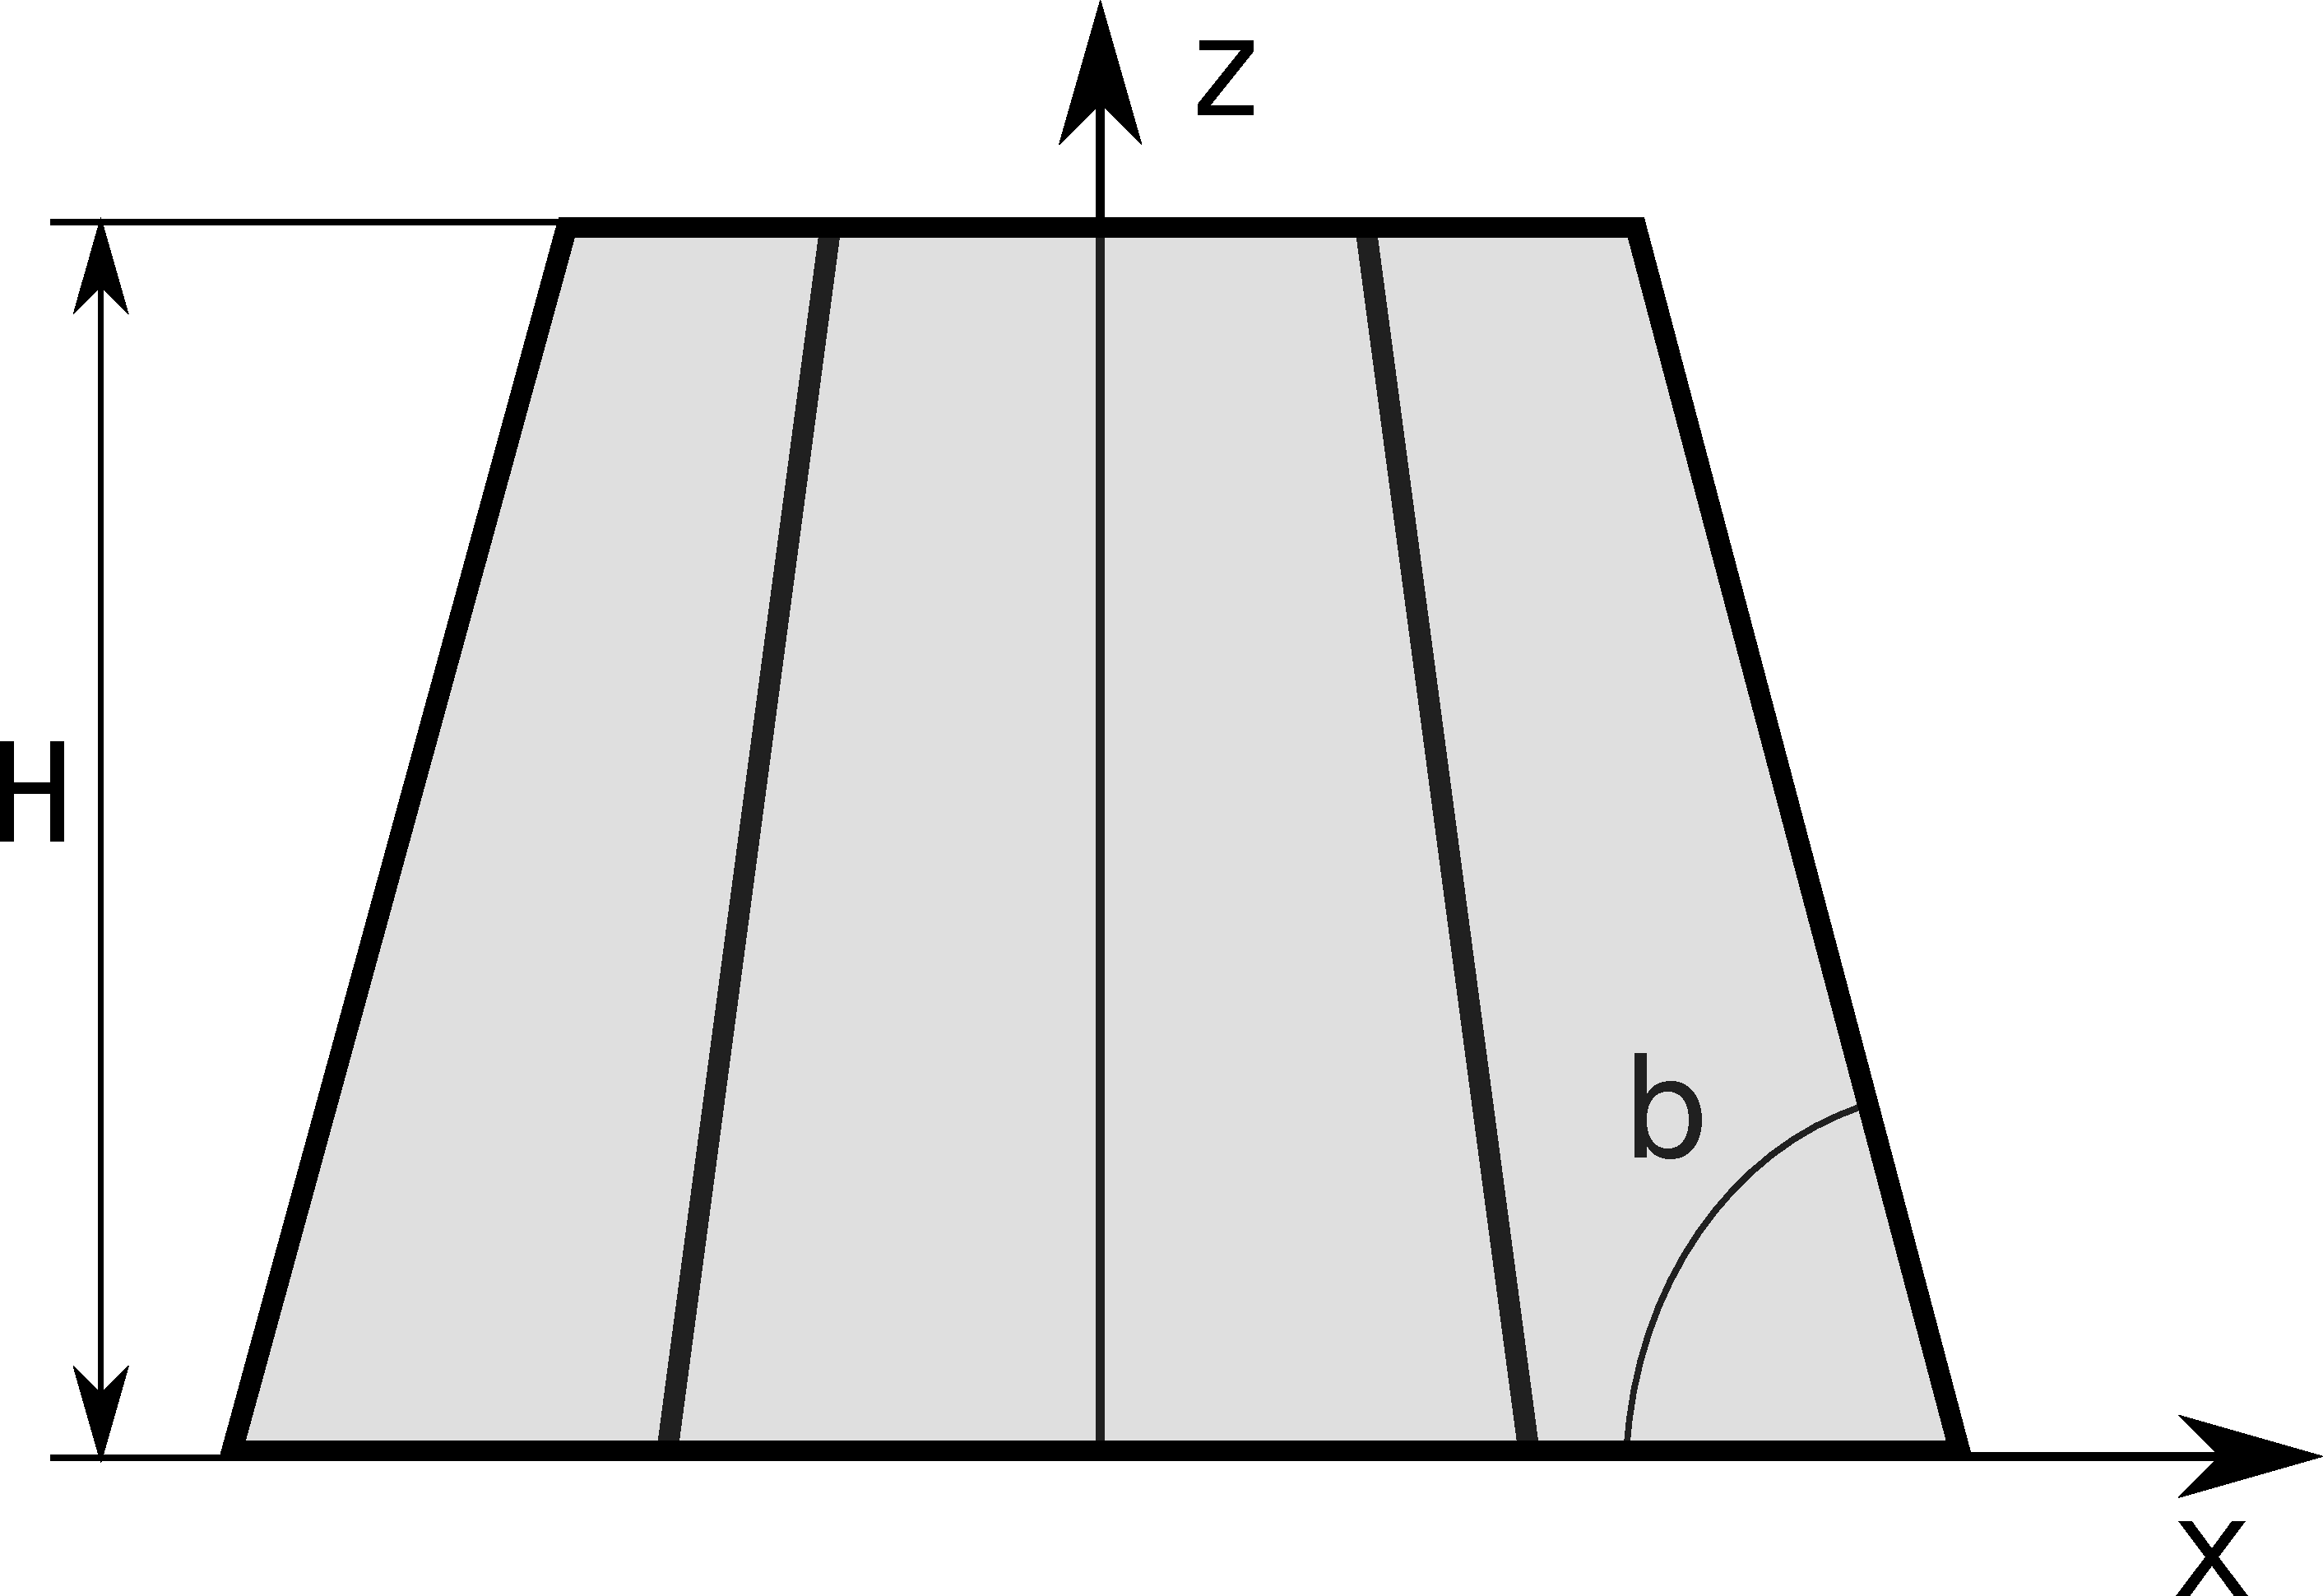
\includegraphics[width=.30\textwidth]{fig/cuts/Cone62dxz.pdf}}}
\hfill
\caption{A truncated hexagonal pyramid.}
\end{figure}

\FloatBarrier
\paragraph{Syntax and parameters}\strut\\[-2ex plus .2ex minus .2ex]
\begin{lstlisting}[language=python, style=eclipseboxed,numbers=none,nolol]
  FormFactorCone6(radius,height, alpha)
\end{lstlisting}
with the parameters
\begin{itemize}
\item \texttt{radius} of the regular hexagonal base, $R$,
\item \texttt{height}, $H$,
\item \texttt{alpha}, between the base and a side face, $\alpha$.
\end{itemize}
Note that the orthographic projection does not show~$\alpha$,
but the angle~$\beta$ between the base and a side edge.
They are related through $\sqrt{3}\tan \alpha = 2 \tan \beta$.
The following is written more conveniently in terms of~$\beta$.
The parameters must fulfill
\begin{displaymath}
  H \le (\tan\beta)R.
\end{displaymath}

\paragraph{Form factor etc}\strut\\
Notation:
\begin{equation*}
  R_H \coloneqq R-\frac{H}{\tan\beta},\quad
  \tilde{q}_x \coloneqq \frac{1}{2}q_y,\quad
  \tilde{q}_y \coloneqq \frac{\sqrt{3}}{2}q_y,\quad
  \tilde{q}_z \coloneqq (\tan\beta) q_z.
\end{equation*}
Results:
\begin{equation*}
  F = \frac{\sqrt{3}\, \e^{i\tilde q_z R}}{\tilde q_y ^2 - \tilde q_x^2}
    \int_{R_H}^R\!\d\rho\, \e^{-i\tilde q_z \rho}
\Big[\rho\tilde q_y \sinc(\tilde q_x\rho)\sin(\tilde q_y\rho)
+\cos(2\tilde q_x\rho)-\cos(\tilde q_y \rho)\cos(\tilde q_x\rho) \Big],
\end{equation*}
\begin{equation*}
  V = \tan\beta  \left( R^3- R_H^3 \right),
\end{equation*}
\begin{equation*}
  S =\dfrac{3\sqrt{3}R^2}{2}.
\end{equation*}

\paragraph{Example}\strut\\
Figure~\ref{fig:FFCone6Ex} shows the normalized intensity
$|F|^2/V^2$, computed with $R=10$~nm, $H=13$~nm, and
$\alpha=60^{\circ}$.

\begin{figure}[H]
\begin{center}
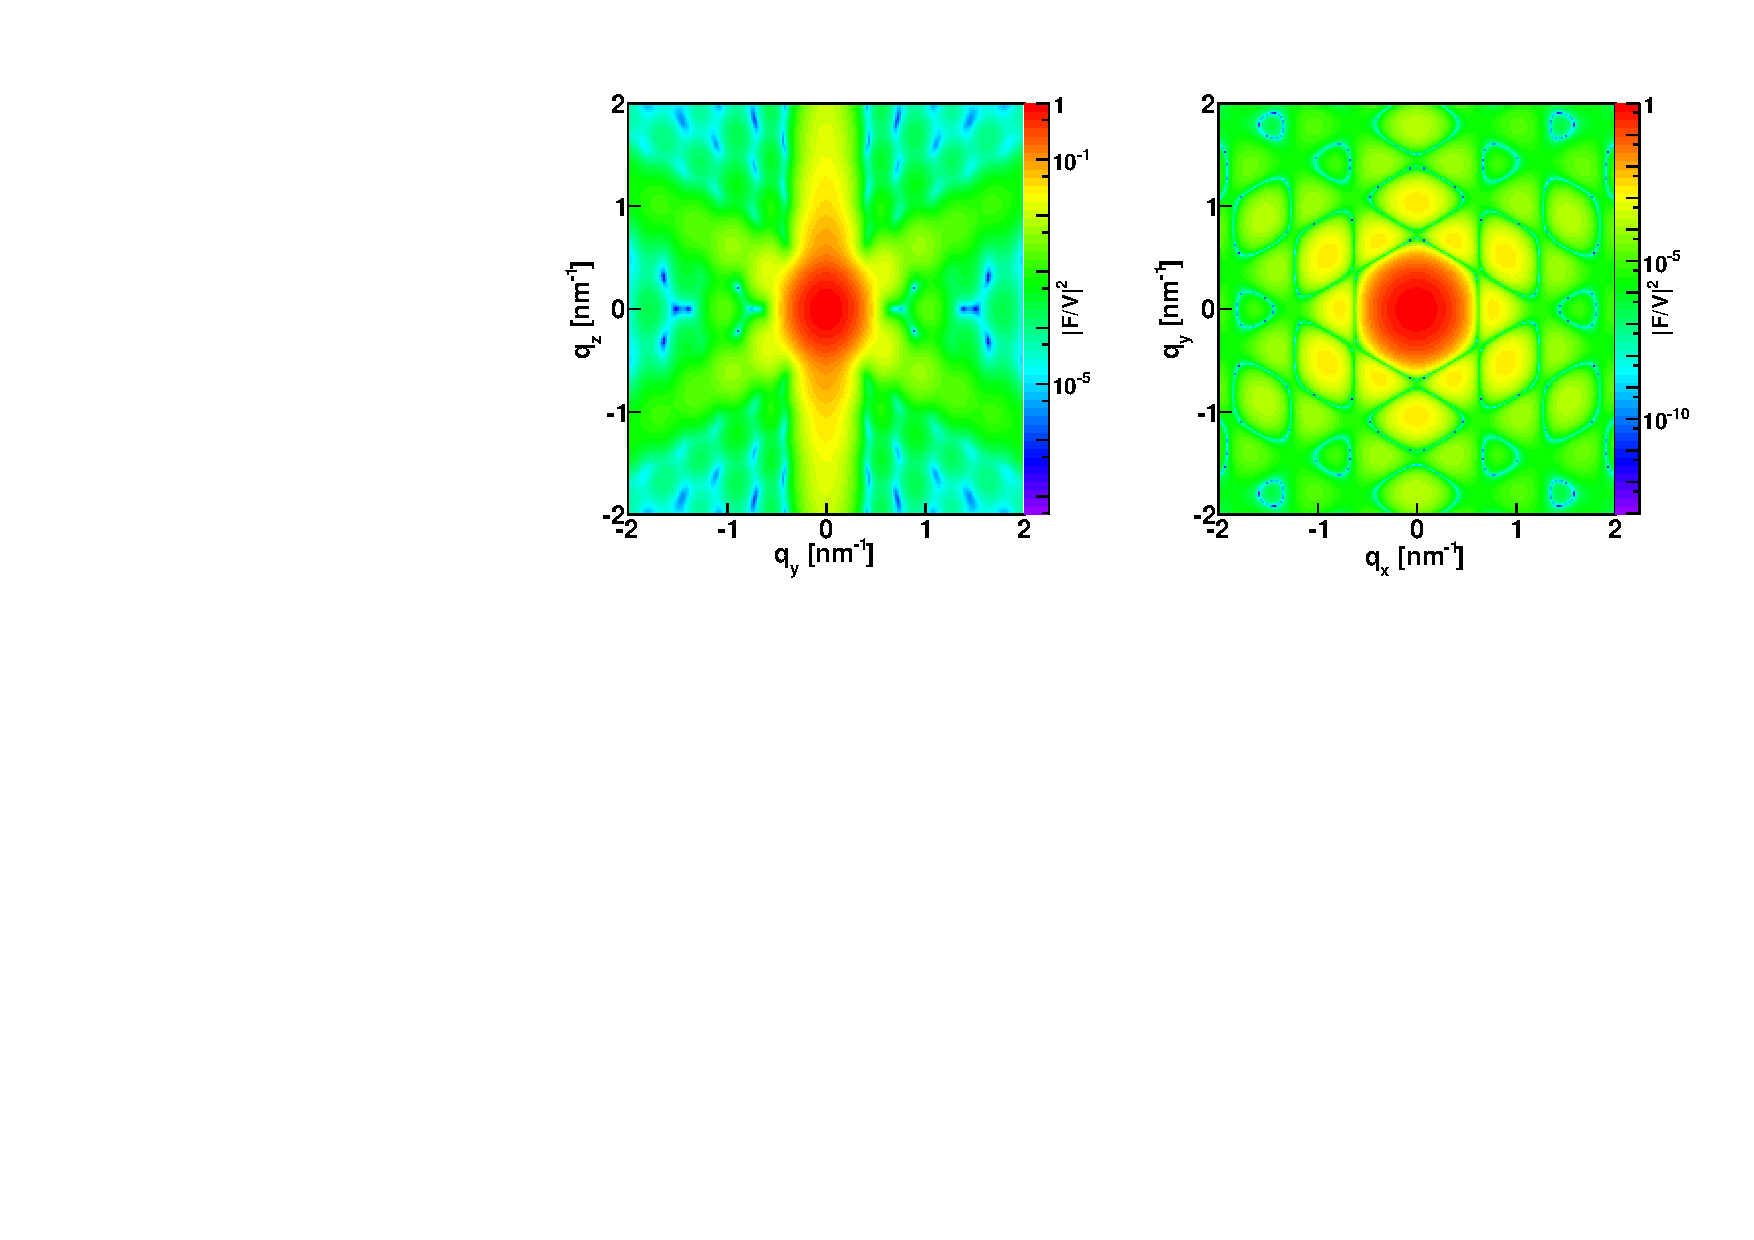
\includegraphics[angle=-90,width=\textwidth]{fig/ff/figffcone6.pdf}
\end{center}
\caption{Normalized intensity for the form factor of a Cone6 plotted against ($q_y$, $q_z$) and ($q_x$, $q_y$) and computed with \Code{FormFactorCone6(10.*nanometer, 13.*nanometer, 60.*degree)}.}
\label{fig:FFCone6Ex}
\end{figure}

\paragraph{References}\strut\\
Hopefully agrees with \E{Cone6} form factor of \IsGISAXS\
\cite[Eq.~2.32]{Laz08} \cite[Eq.~222]{ReLL09},
except for different parametrization.

%-------------------------------------------------------------------------------
\clearpage
\subsection{Cuboctahedron} \label{sec:Cuboctahedron}
  \index{Cuboctahedron (form factor)}
  \index{FormFactorCuboctahedron@\Code{FormFactorCuboctahedron}}
%-------------------------------------------------------------------------------

\paragraph{Real-space geometry}\strut\\

\begin{figure}[H]
\hfill
\subfigure[Perspective]{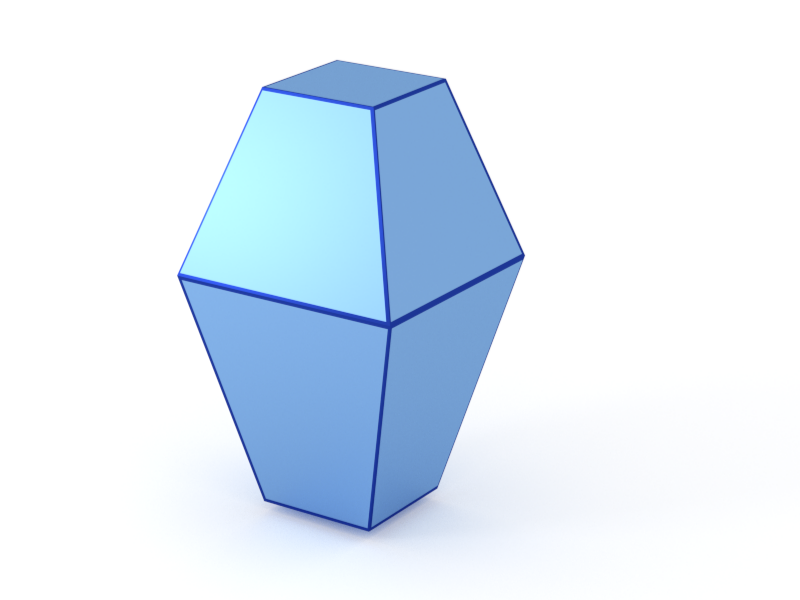
\includegraphics[width=.24\textwidth]{fig/blue/Cuboctahedron3d.png}}
\hfill
\subfigure[Top view]{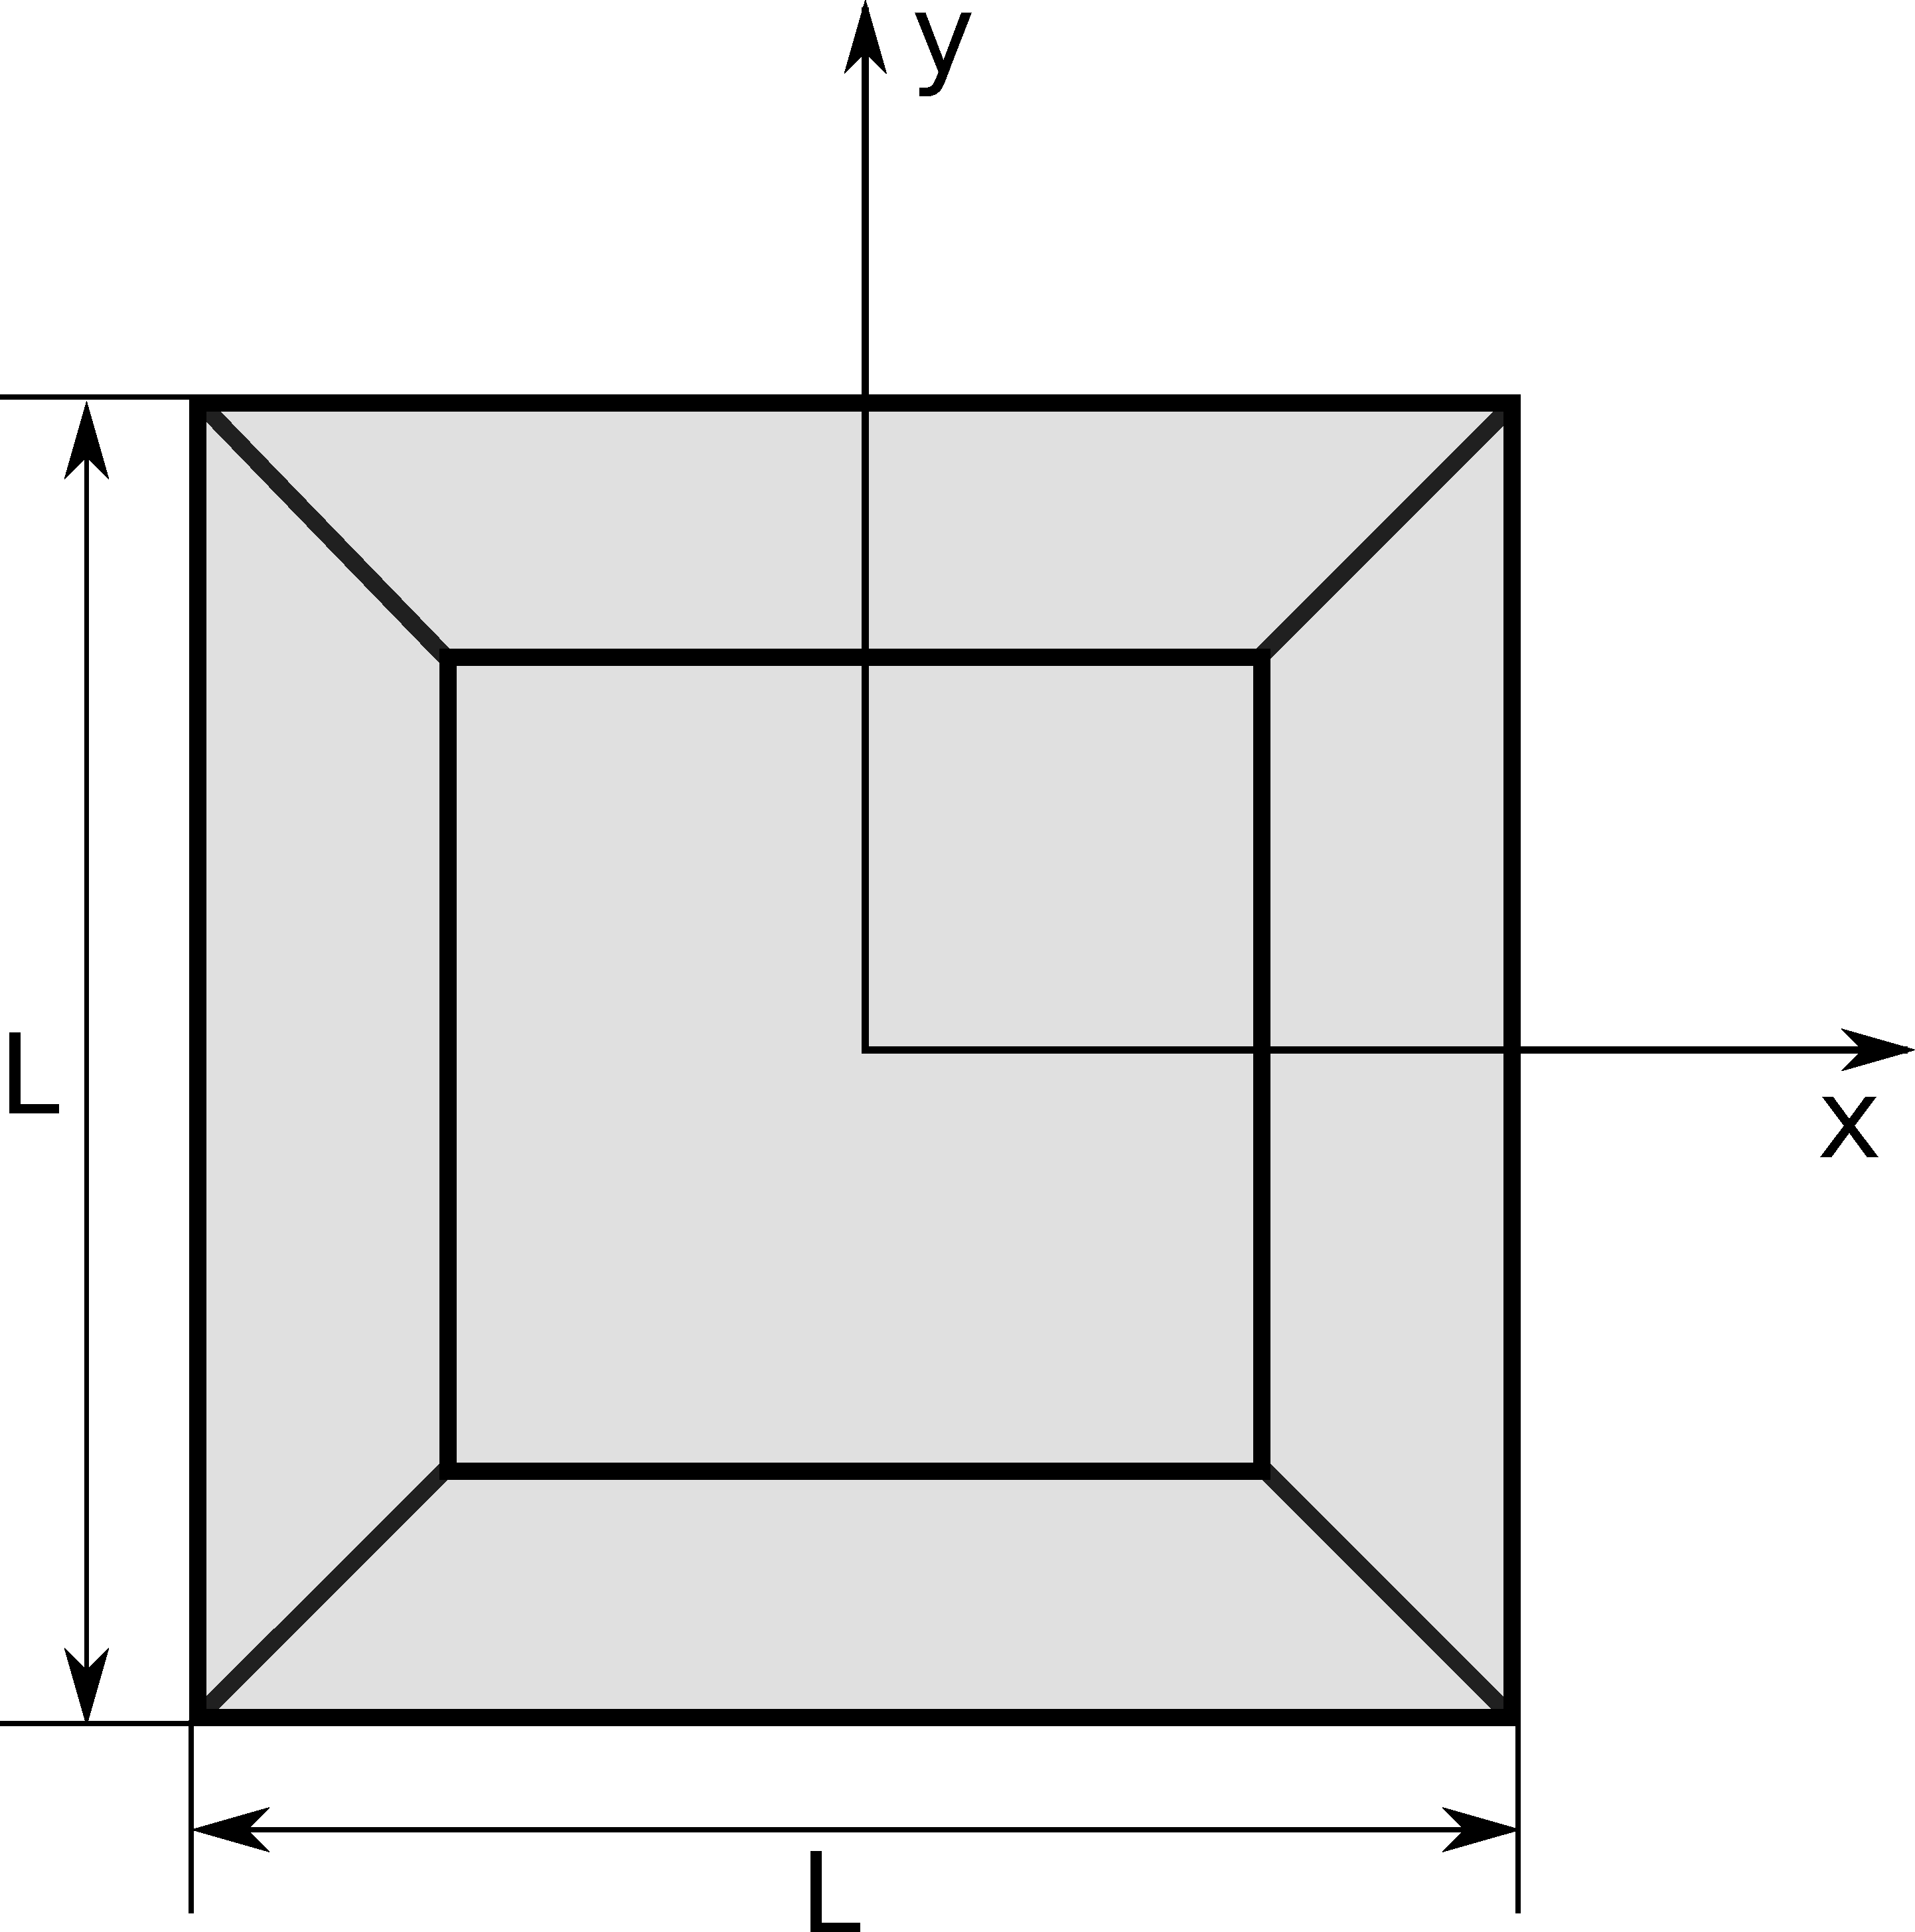
\includegraphics[width=.30\textwidth]{fig/cuts/Cuboctahedron2dxy.pdf}}
\hfill
\subfigure[Side view]{\raisebox{2mm}{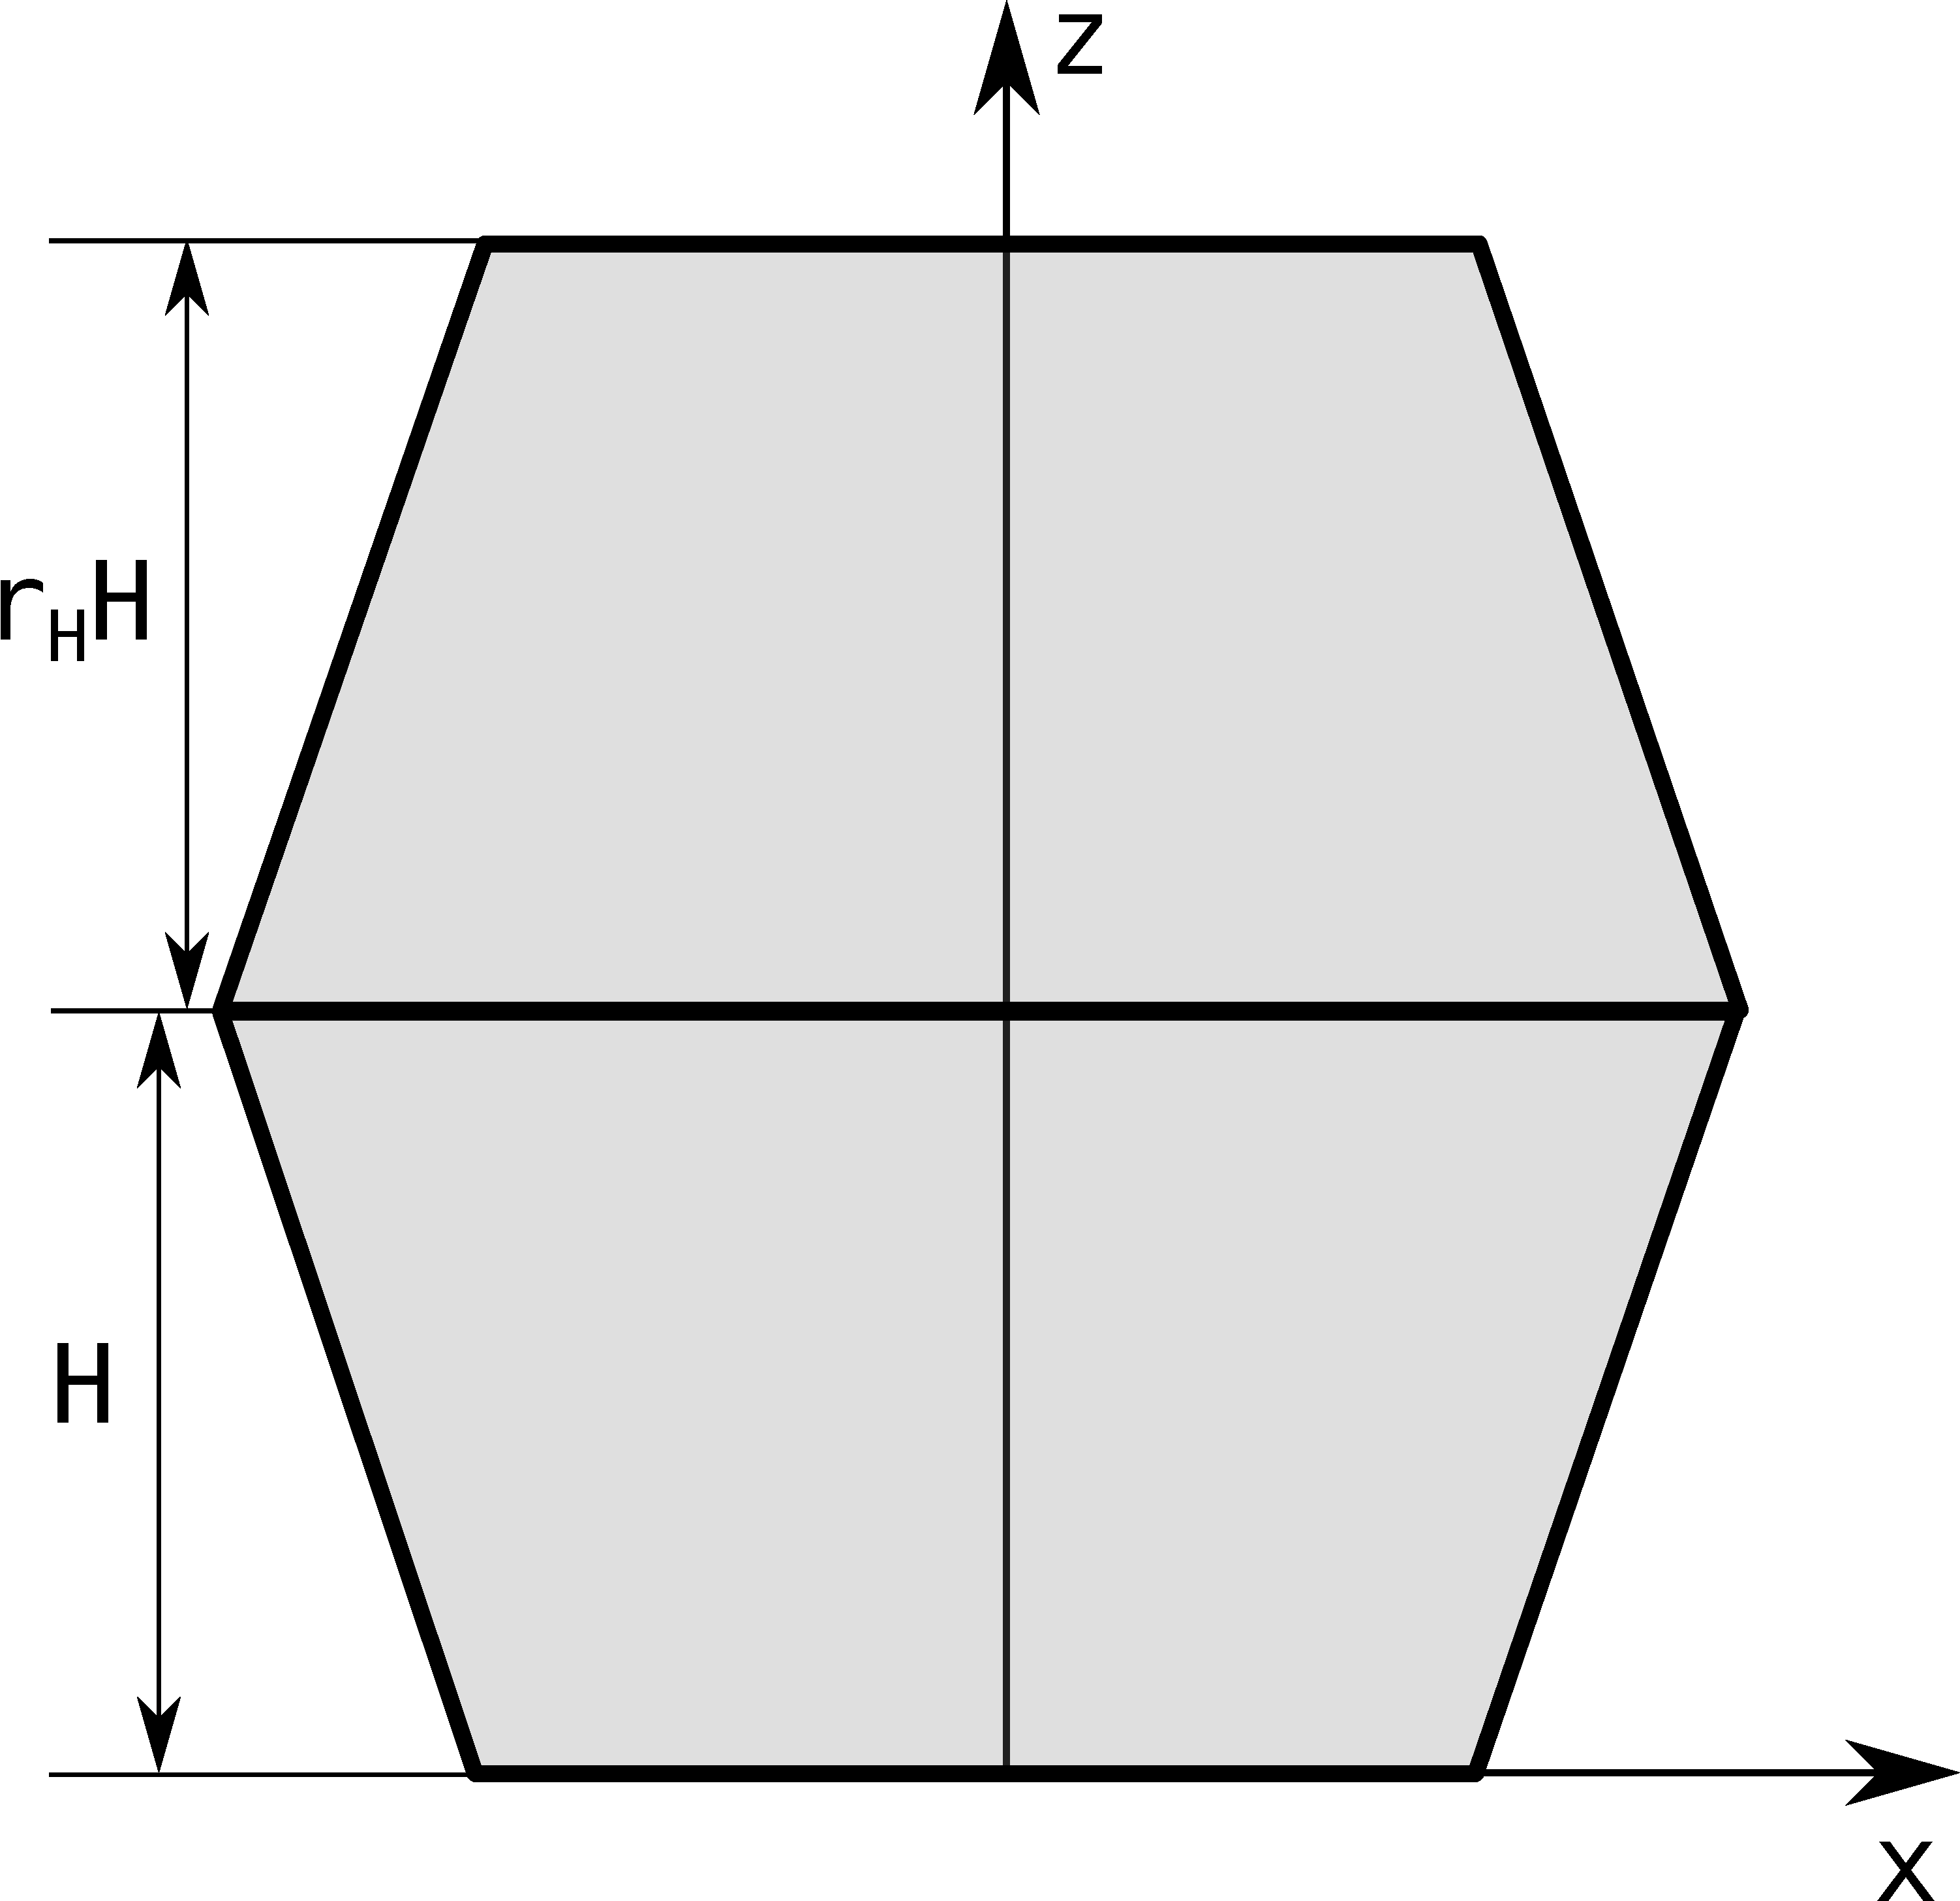
\includegraphics[width=.30\textwidth]{fig/cuts/Cuboctahedron2dxz.pdf}}}
\hfill
\caption{A compound of two truncated pyramids with a common square base
and opposite orientations.}
\end{figure}

\FloatBarrier

\paragraph{Syntax and parameters}\strut\\[-2ex plus .2ex minus .2ex]
\begin{lstlisting}[language=python, style=eclipseboxed,numbers=none,nolol]
  FormFactorCuboctahedron(length, height, height_ratio, alpha)
\end{lstlisting}
with the parameters
\begin{itemize}
\item \texttt{length} of the shared square base, $L$,
\item \texttt{height} of the bottom pyramid, $H$,
\item \texttt{height\_ratio} between the top and the bottom pyramid, $r_H$,
\item \texttt{alpha}, angle between the base and a side face, $\alpha$.
\end{itemize}
They must fulfill
\begin{displaymath}
  H \le \frac{\tan\alpha}{2} L
  \quad\text{and}\quad
  r_h H \le \frac{\tan\alpha}{2} L.
\end{displaymath}


\paragraph{Form factor etc}\strut\\
Using the form factor of a square pyramid $F_\text{Py}$
(Sect.~\ref{sec:Pyramid}):
\begin{equation*}
F=\exp(iq_zH)\Big[F_\text{Py}(q_x,q_y, q_z, L, r_H H,\alpha)
                 +F_\text{Py}(q_x, q_y, -q_z, L, H, \alpha))\Big],
\end{equation*}
\begin{equation*}
  V= \dfrac{1}{6} \tan(\alpha)L^3 \Big[ 2
         - \Big(1 - \dfrac{2H }{L\tan(\alpha)} \Big)^3
           - \Big(1 - \dfrac{2 r_H
             H}{L\tan(\alpha) }\Big)^3\Big],
\end{equation*}
\begin{equation*}
  S =L^2.
\end{equation*}

\paragraph{Example}\strut\\
Figure~\ref{fig:FFcuboctahEx} shows the normalized intensity $|F|^2/V^2$, computed with $L=20$~nm, $H=13$~nm, $r_H=0.7$, and $\alpha=60^{\circ}$.
\begin{figure}[H]
\begin{center}
\includegraphics[angle=-90,width=\textwidth]{fig/ff/figffcuboctah.pdf}
\end{center}
\caption{Normalized intensity for the form factor of a cuboctahedron plotted against ($q_y$, $q_z$) and  ($q_x$, $q_y$) and computed with \Code{FormFactorCuboctahedron(20.*nanometer, 13.*nanometer, 0.7, 60.*degree)}.}
\label{fig:FFcuboctahEx}
\end{figure}

\paragraph{References}\strut\\
Agrees with \E{Cuboctahedron} form factor of \IsGISAXS\
\cite[Eq.~2.34]{Laz08} \cite[Eq.~218]{ReLL09},
except for different parametrization $L=2R_{\rm{\Code{IsGISAXS}}}$.

%-------------------------------------------------------------------------------
\clearpage
\subsection{Cylinder} \label{sec:Cylinder}
  \index{Cylinder (form factor)}
  \index{FormFactorCylinder@\Code{FormFactorCylinder}}
%-------------------------------------------------------------------------------
 
\paragraph{Real-space geometry}\strut\\

\begin{figure}[H]
\hfill
\subfigure[Perspective]{\includegraphics[width=.24\textwidth]{fig/blue/Cylinder3d.png}}
\hfill
\subfigure[Top view]{\includegraphics[width=.30\textwidth]{fig/cuts/Cylinder2dxy.pdf}}
\hfill
\subfigure[Side view]{\raisebox{-2.5mm}{\includegraphics[width=.30\textwidth]{fig/cuts/Cylinder2dxz.pdf}}}
\hfill
\caption{An upright circular cylinder.}
\end{figure}

\paragraph{Syntax and parameters}\strut\\[-2ex plus .2ex minus .2ex]
\begin{lstlisting}[language=python, style=eclipseboxed,numbers=none,nolol]
  FormFactorCylinder(radius, height)
\end{lstlisting}
with the parameters
\begin{itemize}
\item \texttt{radius} of the circular base, $R$, 
\item \texttt{height}, $H$.
\end{itemize}


\paragraph{Form factor etc}\strut\\
Notation:
\begin{equation*}
  q_{\parallel} \coloneqq \sqrt{q_x^2+q_y^2}.
\end{equation*}
Results:
\begin{equation*}
  F=  2\pi R^2 H  \sinc\left(q_ z \frac{H}{2}\right) \exp\left(i q_ z \frac{H}{2}\right) 
    \frac{J_1(q_{\parallel} R )}{q_{\parallel} R },
\end{equation*}
\begin{equation*}
  V = \pi R^2 H,
\end{equation*}
\begin{equation*}
  S=\pi R^2.
\end{equation*}

\paragraph{Examples}\strut

\begin{figure}[H]
\begin{center}
\includegraphics[width=\textwidth]{fig/ff2/ff_Cylinder.pdf}
\end{center}
\caption{Normalized intensity $|F|^2/V^2$,
computed with $R=3$~nm and $H=8.8$~nm,
for four different tilt angles~$\vartheta$ (rotation around the $y$ axis).}
\end{figure}

\paragraph{References}\strut\\
Agrees with \E{Cylinder} form factor of \IsGISAXS\
\cite[Eq.~2.27]{Laz08} \cite[Eq.~223]{ReLL09}.

%-------------------------------------------------------------------------------
\clearpage
\subsection{EllipsoidalCylinder} \label{sec:EllipsoidalCylinder} 
  \index{Ellipsoidal cylinder (form factor)}
  \index{Cylinder (form factor)!ellipsoidal}
  \index{FormFactorEllipsoidalCylinder@\Code{FormFactorEllipsoidalCylinder}}
%-------------------------------------------------------------------------------

\paragraph{Real-space geometry}\strut\\

\begin{figure}[H]
\hfill
\subfigure[Perspective]{\includegraphics[width=.24\textwidth]{fig/blue/EllipsoidalCylinder3d.png}}
\hfill
\subfigure[Top view]{\includegraphics[width=.30\textwidth]{fig/cuts/EllipsoidalCylinder2dxy.pdf}}
\hfill
\subfigure[Side view]{\raisebox{4mm}{\includegraphics[width=.30\textwidth]{fig/cuts/EllipsoidalCylinder2dxz.pdf}}}
\hfill
\caption{A upright cylinder whose cross section is an ellipse.}
\end{figure}

\paragraph{Syntax and parameters}\strut\\[-2ex plus .2ex minus .2ex]
\begin{lstlisting}[language=python, style=eclipseboxed,numbers=none,nolol]
  FormFactorEllipsoidalCylinder(radius_a, radius_b, height)
\end{lstlisting}
with the parameters
\begin{itemize}
\item \texttt{radius\_a}, in $x$ direction, $R_a$,
\item \texttt{radius\_b}, in $y$ direction, $R_b$,
\item height $H$.
\end{itemize}


\paragraph{Form factor etc}\strut\\
Notation:
\begin{equation*}
  \gamma \coloneqq \sqrt{(q_x R_a)^2+(q_y R_b)^2}  
\end{equation*}
Results:
\begin{equation*}
F = 2\pi R_a R_b H \exp\left(i\frac{q_z H}{2}\right)
   \sinc\left(\frac{q_z H}{2}\right) \frac{J_1(\gamma)}{\gamma},
\end{equation*}
\begin{equation*}
  V = \pi R_a R_bH,
\end{equation*}
\begin{equation*}
  S = R_a R_b.
\end{equation*}

\paragraph{Example}\strut

\begin{figure}[H]
\begin{center}
\includegraphics[width=\textwidth]{fig/ff2/ff_EllipsoidalCylinder.pdf}
\end{center}
\caption{Normalized intensity $|F|^2/V^2$,
computed with $R_a=6.3$~nm, $R_b=4.2$~nm and $H=3$~nm,
for four different angles~$\omega$ of rotation around the $z$ axis.}
\end{figure}

\paragraph{References}\strut\\
Agrees with the \IsGISAXS\ form factor
\E{Ellipsoid} \cite[Eq.~2.41, wrongly labeled in Fig.~2.4]{Laz08}
or \E{Ellipsoidal Cylinder} \cite[Eq.~224]{ReLL09}.

%-------------------------------------------------------------------------------
\clearpage
\subsection{FullSphere} \label{sec:FullSphere}
  \index{Full sphere (form factor)}
  \index{Sphere (form factor)}
  \index{FormFactorFullSphere@\Code{FormFactorFullSphere}}
%-------------------------------------------------------------------------------

\paragraph{Real-space geometry}\strut\\

\begin{figure}[H]
\hfill
\subfigure[Perspective]{\includegraphics[width=.24\textwidth]{fig/blue/FullSphere3d.png}}
\hfill
\subfigure[Top view]{\includegraphics[width=.30\textwidth]{fig/cuts/FullSphere2dxy.pdf}}
\hfill
\subfigure[Side view]{\raisebox{-2mm}{\includegraphics[width=.30\textwidth]{fig/cuts/FullSphere2dxz.pdf}}}
\hfill
\caption{A full sphere.}
\end{figure}

\FloatBarrier

\paragraph{Syntax and parameters}\strut\\[-2ex plus .2ex minus .2ex]
\begin{lstlisting}[language=python, style=eclipseboxed,numbers=none,nolol]
  FormFactorFullSphere(radius)
\end{lstlisting}
with the parameter
\begin{itemize}
\item \texttt{radius}, $R$.
\end{itemize}


\paragraph{Form factor etc}\strut\\
\begin{equation*}
F = 4\pi R^3 \exp(iq_z R)\frac{\sin(q R) - q R \cos(q R)}{(qR)^3},
\end{equation*}
\begin{equation*}
  V = \dfrac{4\pi}{3}R^3,
\end{equation*}
\begin{equation*}
  S= \pi R^2.
\end{equation*}

\paragraph{Example}\nopagebreak\strut\nopagebreak

\begin{figure}[H]
\begin{center}
\includegraphics[width=0.5\textwidth]{fig/ff2/ff_FullSphere.pdf}
\end{center}
\caption{Normalized intensity $|F|^2/V^2$,
computed with $R=3.9$~nm.}
\end{figure}

\paragraph{References}\strut\\
This form factor, which certainly goes back at least to Lord Rayleigh,
agrees with the \E{Full sphere} of \IsGISAXS
\cite[Eq.~2.36]{Laz08} \cite[Eq.~226]{ReLL09}.

%-------------------------------------------------------------------------------
\clearpage
\subsection{HemiEllipsoid} \label{sec:HemiEllipsoid}  
  \index{Hemi ellipsoid (form factor)}
  \index{Ellipsoid (form factor)!truncated}
  \index{Truncated ellipsoid (form factor)}
  \index{FormFactorHemiEllipsoid@\Code{FormFactorHemiEllipsoid}}
%-------------------------------------------------------------------------------

\paragraph{Real-space geometry}\strut\\

\begin{figure}[H]
\hfill
\subfigure[Perspective]{\includegraphics[width=.24\textwidth]{fig/blue/HemiEllipsoid3d.png}}
\hfill
\subfigure[Top view]{\includegraphics[width=.30\textwidth]{fig/cuts/HemiEllipsoid2dxy.pdf}}
\hfill
\subfigure[Side view]{\raisebox{5mm}{\includegraphics[width=.30\textwidth]{fig/cuts/HemiEllipsoid2dxz.pdf}}}
\hfill
\caption{An horizontally oriented ellipsoid, truncated at the central plane.}
\end{figure}

\paragraph{Syntax and parameters}\strut\\[-2ex plus .2ex minus .2ex]
\begin{lstlisting}[language=python, style=eclipseboxed,numbers=none,nolol]
  FormFactorHemiEllipsoid(radius_a, radius_b, height)
\end{lstlisting}
with the parameters
\begin{itemize}
\item \texttt{radius\_a}, in $x$ direction, $R_a$,
\item \texttt{radius\_b}, in $y$ direction, $R_b$,
\item \texttt{height}, equal to radius in $z$ direction, $H$
\end{itemize}


\paragraph{Form factor etc}\strut\\
Notation:
\begin{equation*}
 r_{a,z} \coloneqq R_a \sqrt{1-\left(\dfrac{z}{H} \right)^2},\quad
 r_{b,z} \coloneqq R_b \sqrt{1-\left(\dfrac{z}{H} \right)^2}, \quad
 \gamma_z =\sqrt{(q_x r_{a,z})^2+(q_y r_{b,z})^2}.
\end{equation*}
Results:
\begin{equation*}
  F = 2\pi \int_0^{H} \!\d z\, r_{a,z} r_{b,z}
                               \frac{J_1(\gamma_z)}{\gamma_z}\exp(iq_z z),
\end{equation*}
\begin{equation*}
  V = \dfrac{2}{3}\pi R_a R_bH,
\end{equation*}
\begin{equation*}
  S =\pi R_a R_b.
\end{equation*}

\paragraph{Example}\strut

\begin{figure}[H]
\begin{center}
\includegraphics[width=\textwidth]{fig/ff2/ff_HemiEllipsoid.pdf}
\end{center}
\caption{Normalized intensity $|F|^2/V^2$,
computed with $R_a=10$~nm, $R_b=3.8$~nm and $H=3.2$~nm,
for four different angles~$\omega$ of rotation around the $z$ axis.}
\end{figure}

\paragraph{References}\strut\\
Agrees with the \IsGISAXS\ form factor
\E{Anisotropic hemi-ellipsoid}
\cite[Eq.~2.42, with wrong sign in the $z$-dependent phase factor]{Laz08}
or \E{Hemi-spheroid} \cite[Eq.~229]{ReLL09}.

%-------------------------------------------------------------------------------
\clearpage
\subsection{FullSpheroid} \label{sec:FullSpheroid}
  \index{Full spheroid (form factor)}
  \index{Spheroid (form factor)}
  \index{FormFactorFullSpheroid@\Code{FormFactorFullSpheroid}}
%-------------------------------------------------------------------------------

\paragraph{Real-space geometry}\strut\\

\begin{figure}[H]
\hfill
\subfigure[Perspective]{\includegraphics[width=.24\textwidth]{fig/blue/FullSpheroid3d.png}}
\hfill
\subfigure[Top view]{\includegraphics[width=.30\textwidth]{fig/cuts/FullSpheroid2dxy.pdf}}
\hfill
\subfigure[Side view]{\raisebox{-3mm}{\includegraphics[width=.30\textwidth]{fig/cuts/FullSpheroid2dxz.pdf}}}
\hfill
\caption{A full spheroid, generated by rotating an ellipse around the vertical axis.}
\end{figure}

\FloatBarrier

\paragraph{Syntax and parameters}\strut\\[-2ex plus .2ex minus .2ex]
\begin{lstlisting}[language=python, style=eclipseboxed,numbers=none,nolol]
  FormFactorFullSpheroid(radius,height)
\end{lstlisting}
with the parameters
\begin{itemize}
\item \texttt{radius}, $R$,
\item \texttt{height}, $H$.
\end{itemize}


\paragraph{Form factor etc}\strut\\
Notation:
\begin{equation*}
 R_z \coloneqq R\sqrt{1-\frac{4z^2}{H^2}},\quad
 q_\plll \coloneqq \sqrt{q_x^2+q_y^2}.
\end{equation*}
Results:
\begin{equation*}
  F = 4\pi \exp(i q_z H/2) \int_0^{H/2} \!\d z\,
     R_z^2 \frac{J_1(q_{\parallel}R_z)}{q_{\parallel}R_z} \cos(q_z z),
\end{equation*}
\begin{equation*}
  V =\dfrac{2}{3}R^2H,
\end{equation*}
\begin{equation*}
  S =\pi R^2.
\end{equation*}

\paragraph{Example}\strut

\begin{figure}[H]
\begin{center}
\includegraphics[width=0.5\textwidth]{fig/ff2/ff_FullSpheroid.pdf}
\end{center}
\caption{Normalized intensity $|F|^2/V^2$,
computed with $R=3.5$~nm and $H=9.8$~nm.}
\end{figure}

\paragraph{References}\strut\\
Agrees with the \E{Full spheroid} form factor of \IsGISAXS\
\cite[Eq.~2.37]{Laz08} \cite[Eq.~227]{ReLL09},
with corrected volume formula.

%\subsection{References}
%The expression is identical to \Code{IsGISAXS} manual. In the code,
%the integration is over $[-H/2, H/2]$ with $\exp(iq_z z)$ instead of
%the cosine.
%In \Code{IsGISAXS}, factor 4 instead of 2 in the expression of the
%volume. In the code there is also a problem with an extra factor 2 in the function to integrate.


%-------------------------------------------------------------------------------
\clearpage
\subsection{Prism3 (triangular)} \label{sec:Prism3}
  \index{Prism (form factor)!triangular (Prism3)}
  \index{FormFactorPrism3@\Code{FormFactorPrism3}}
%-------------------------------------------------------------------------------

\paragraph{Real-space geometry}\strut\\

\Work{probably the $xy$ view needs to be rotated by 30$^\circ$}

\begin{figure}[H]
\hfill
\subfigure[Perspective]{\includegraphics[width=.24\textwidth]{fig/blue/Prism33d.png}}
\hfill
\subfigure[Top view]{\includegraphics[width=.30\textwidth]{fig/cuts/Prism32dxy.pdf}}
\hfill
\subfigure[Side view]{\raisebox{2mm}{\includegraphics[width=.30\textwidth]{fig/cuts/Prism32dxz.pdf}}}
\hfill
\caption{A prism based on an equilateral triangle.}
\end{figure}

\FloatBarrier

\paragraph{Syntax and parameters}\strut\\[-2ex plus .2ex minus .2ex]
\begin{lstlisting}[language=python, style=eclipseboxed,numbers=none,nolol]
  FormFactorPrism3(length, height)
\end{lstlisting}
with the parameters
\begin{itemize}
\item \texttt{length} of one base edge, $L$,
\item \texttt{height}, $H$.
\end{itemize}


\paragraph{Form factor etc}\strut\\
\begin{align*}
F &= \frac{2 \sqrt{3}}{q_x^2-3q_y^2} 
     \exp\left(-i q_y\frac{L}{2\sqrt{3}}\right)
    \left[\exp\left(i \sqrt{3} q_y \frac{L}{2} \right)-\cos\left(q_x \frac{L}{2}\right)
    -i \sqrt{3} q_y \frac{L}{2} \sinc\left(q_x \frac{L}{2}\right) \right] \\
  &
  \times  H \sinc\left(q_z \frac{H}{2} \right) \exp\left(i q_z \frac{H}{2}\right),
\end{align*}
\begin{equation*}
  V= \dfrac{\sqrt{3}}{4} H L^2,
\end{equation*}
\begin{equation*}
  S =\dfrac{\sqrt{3}}{4}L^2.
\end{equation*}

\paragraph{Example}\strut

\begin{figure}[H]
\begin{center}
\includegraphics[width=\textwidth]{fig/ff2/ff_prism3.pdf}
\end{center}
\caption{Normalized intensity $|F|^2/V^2$,
computed with $R=13.8$~nm and $H=3$~nm,
for four different angles~$\omega$ of rotation around the $z$ axis.}
\label{fig:FFprism3Ex}
\end{figure}

\paragraph{References}\strut\\
Agrees with \E{Prism3} form factor of \IsGISAXS\
\cite[Eq.~2.29]{Laz08} \cite[Eq.~219]{ReLL09},
except for the definition of parameter $L= 2 R_{\rm{\Code{IsGISAXS}}}$.

%-------------------------------------------------------------------------------
\clearpage
\subsection{Prism6 (hexagonal)} \label{sec:Prism6}
  \index{Prism (form factor)!hexagonal (Prism6)}
  \index{FormFactorPrism6@\Code{FormFactorPrism6}}
%-------------------------------------------------------------------------------

\paragraph{Real-space geometry}\strut\\

\begin{figure}[H]
\hfill
\subfigure[Perspective]{\includegraphics[width=.24\textwidth]{fig/blue/Prism63d.png}}
\hfill
\subfigure[Top view]{\includegraphics[width=.30\textwidth]{fig/cuts/Prism62dxy.pdf}}
\hfill
\subfigure[Side view]{\raisebox{-3mm}{\includegraphics[width=.30\textwidth]{fig/cuts/Prism62dxz.pdf}}}
\hfill
\caption{A prism based on a regular hexagon.}
\end{figure}

\FloatBarrier

\paragraph{Syntax and parameters}\strut\\[-2ex plus .2ex minus .2ex]
\begin{lstlisting}[language=python, style=eclipseboxed,numbers=none,nolol]
  FormFactorPrism6(radius, height)
\end{lstlisting}
with the parameters
\begin{itemize}
\item \texttt{radius} of the hexagonal base, $R$,
\item \texttt{height}, $H$.
\end{itemize}


\paragraph{Form factor etc}\strut\\
\begin{align*}
F &= \frac{4H\sqrt{3}}{3q_y^2 - q_x^2}
\sinc\left(q_z\frac{H}{2}\right) \exp\left(-i q_z\frac{ H}{2}\right)\times\\
&\left\{\frac{3q_y^2R^2}{4} \sinc\left(\frac{q_x
  R}{2}\right)\sinc\left(\frac{\sqrt{3}q_yR }{2}\right)+ \cos(q_x R)-\cos\left(q_y
\frac{\sqrt{3}R}{2}\right) \cos\left(\frac{q_x R}{2}\right)\right\},
\end{align*}
\begin{equation*}
  V = \dfrac{3\sqrt{3}}{2}H R^2,
\end{equation*}
\begin{equation*}
  S =\dfrac{3\sqrt{3}R^2}{2}.
\end{equation*}

\paragraph{Examples}\strut

\begin{figure}[H]
\begin{center}
\includegraphics[width=\textwidth]{fig/ff2/ff_prism6.pdf}
\end{center}
\caption{Normalized intensity $|F|^2/V^2$,
computed with $R=5.7$~nm and $H=3$~nm,
for four different angles~$\omega$ of rotation around the $z$ axis.}
\label{fig:FFprism6Ex}
\end{figure}

\paragraph{References}\strut\\
Corresponds to \E{Prism6} form factor of \IsGISAXS\
\cite[Eq.~2.31]{Laz08} \cite[Eq.~221]{ReLL09},
which has different parametrization
and lacks a factor $H$ in $F(\q)$.

%-------------------------------------------------------------------------------
\clearpage
\subsection{Pyramid (square-based)}\label{sec:Pyramid}
  \index{Pyramid (form factor)!square}
  \index{Truncated pyramid (form factor)!square}
  \index{FormFactorPyramid@\Code{FormFactorPyramid}}
%-------------------------------------------------------------------------------

\paragraph{Real-space geometry}\strut\\

\begin{figure}[H]
\hfill
\subfigure[Perspective]{\includegraphics[width=.24\textwidth]{fig/blue/Pyramid3d.png}}
\hfill
\subfigure[Top view]{\includegraphics[width=.30\textwidth]{fig/cuts/Pyramid2dxy.pdf}}
\hfill
\subfigure[Side view]{\raisebox{2mm}{\includegraphics[width=.30\textwidth]{fig/cuts/Pyramid2dxz.pdf}}}
\hfill
\caption{A truncated pyramid with a square base.}
\end{figure}

\FloatBarrier

\paragraph{Syntax and parameters}\strut\\[-2ex plus .2ex minus .2ex]
\begin{lstlisting}[language=python, style=eclipseboxed,numbers=none,nolol]
  FormFactorPyramid(length, height, alpha)
\end{lstlisting}
with the parameters
\begin{itemize}
\item \texttt{length} of one edge of the square base, $L$,  
\item \texttt{height}, $H$,
\item \texttt{alpha}, angle between the base and a side face, $\alpha$,
\end{itemize}
They must fulfill
\begin{displaymath}
  H \le \frac{\tan\alpha}{2}L.
\end{displaymath}


\paragraph{Form factor etc}\strut\\
Notation:
\begin{displaymath}
  \ell\coloneqq L/2,\quad
  h\coloneqq H/2,\quad
  f_\pm(z)\coloneqq \exp(\pm i z)\sinc(z).
\end{displaymath}
Results:
\begin{equation*}
\begin{array}{@{}l@{}l@{}}
\DS F=
\frac{H}{q_xq_y} \Big\{
   &+\DS  f_+\left(\left(\frac{q_x-q_y}{\tan\alpha} +q_z\right)h\right)
        \exp(-i(q_x-q_y)\ell)
\\[3.6ex]
   &\DS+ f_-\left(\left(\frac{q_x-q_y}{\tan\alpha} -q_z\right)h\right)
        \exp(+i(q_x-q_y)\ell)
\\[3.6ex]
   &\DS- f_+\left(\left(\frac{q_x+q_y}{\tan\alpha} +q_z\right)h\right)
        \exp(-i(q_x+q_y)\ell)
\\[3.6ex]
   &\DS- f_-\left(\left(\frac{q_x+q_y}{\tan\alpha} -q_z\right)h\right)
        \exp(+i(q_x+q_y)\ell)
\Big\},
\end{array}
\end{equation*}
\begin{equation*}
  V= H \Big[L^2 - \frac{2LH}{\tan\alpha} + \dfrac{4}{3} \dfrac{H^2}{\tan^2\alpha}\Big].
\end{equation*}
\begin{equation*}
  S=L^2.
\end{equation*}
\begin{equation*}
  V = \dfrac{1}{6}  L^3 \tan\alpha\left[ 1
             - \left(1 - \dfrac{2H}{L\tan\alpha}\right)^3 \right],,
\end{equation*}
\begin{equation*}
  S = L^2.
\end{equation*}

\paragraph{Examples}\strut

\begin{figure}[H]
\begin{center}
%\includegraphics[angle=-90,width=\textwidth]{fig/ff/figffpyramid.pdf}
\includegraphics[width=\textwidth]{fig/ff2/ff_pyramid.pdf}
\end{center}
\caption{Normalized intensity $|F|^2/V^2$,
computed with $L=10$~nm, $H=4.2$~nm and $\alpha=60^{\circ}$,
for four different angles~$\omega$ of rotation around the $z$ axis.}
\end{figure}

\paragraph{References}\strut\\
Corresponds to \E{Pyramid} form factor of \IsGISAXS\
\cite[Eq.~2.31]{Laz08} \cite[Eq.~221]{ReLL09},
with different parametrization $L=2R_{\rm{\Code{IsGISXAXS}}}$,
with correction of a sign error,
and with a more compact form of $F(\q)$.

%-------------------------------------------------------------------------------
\clearpage
\subsection{Ripple1 (sinusoidal)} \label{sec:Ripple1}  
  \index{Ripple (form factor)!sinusoidal (Ripple1)}
  \index{Sinusoidal ripple (form factor)}
  \index{FormFactorRipple1@\Code{FormFactorRipple1}}
%-------------------------------------------------------------------------------

\paragraph{Real-space geometry}\strut\\

\begin{figure}[H]
\hfill
\subfigure[Perspective]{\includegraphics[width=.24\textwidth]{fig/blue/Ripple13d.png}}
\hfill
\subfigure[Top view]{\includegraphics[width=.30\textwidth]{fig/cuts/Ripple12dxy.pdf}}
\hfill
\subfigure[Side view]{\includegraphics[width=.30\textwidth]{fig/cuts/Ripple12dyz.pdf}}
\hfill
\caption{An infinite ripple with a sinusoidal profile.}
\end{figure}

\paragraph{Syntax and parameters}\strut\\[-2ex plus .2ex minus .2ex]
\begin{lstlisting}[language=python, style=eclipseboxed,numbers=none,nolol]
  FormFactorRipple1(length, width, height)
\end{lstlisting}
with the parameters
\begin{itemize}
\item \texttt{length}, $L$, 
\item \texttt{width}, $W$, 
\item \texttt{height}, $H$. 
\end{itemize}


\paragraph{Form factor etc}\strut\\
\begin{align*}
F &=L \cdot \frac{W}{\pi}\cdot \sinc\left(\frac{q_xL}{2}\right)\times \\
&\int_0^H\!\d z\, \arccos\left(\frac{2z}{H}-1\right)\sinc\left[\frac{q_yW}{2\pi}\arccos\left(\frac{2z}{H} - 1\right)\right]\exp\left(iq_zz\right),
\end{align*}
\begin{equation*}
  V = \dfrac{L W H}{2},
\end{equation*}
\begin{equation*}
  S = L W.
\end{equation*}

\paragraph{Example}\strut\\
Figure~\ref{fig:FFripple1Ex} shows the normalized intensity
$|F|^2/V^2$, computed with $L=27$~nm, $W=20$~nm and $H=14$~nm.

\begin{figure}[H]
\begin{center}
\includegraphics[angle=-90,width=\textwidth]{fig/ff/figffripple1.pdf}
\end{center}
\caption{Normalized intensity for the form factor of a ripple1
  $|F|^2/V^2$, plotted against ($q_y$, $q_z$) and  ($q_x$, $q_y$)
  computed with \Code{FormFactorRipple1(27.*nanometer, 20.*nanometer, 14.*nanometer)}.}
\label{fig:FFripple1Ex}
\end{figure}


%-------------------------------------------------------------------------------
\clearpage
\subsection{Ripple2 (saw-tooth)} \label{sec:Ripple2}  
  \index{Ripple (form factor)!saw-tooth (Ripple2)}
  \index{Saw-tooth ripple (form factor)}
  \index{FormFactorRipple2@\Code{FormFactorRipple2}}
%-------------------------------------------------------------------------------

\paragraph{Real-space geometry}\strut\\

\begin{figure}[H]
\hfill
\subfigure[Perspective]{\includegraphics[width=.24\textwidth]{fig/blue/Ripple23d.png}}
\hfill
\subfigure[Top view]{\includegraphics[width=.30\textwidth]{fig/cuts/Ripple22dxy.pdf}}
\hfill
\subfigure[Side view]{\includegraphics[width=.30\textwidth]{fig/cuts/Ripple22dyz.pdf}}
\hfill
\caption{An infinite ripple with an asymmetric saw-tooth profile.}
\end{figure}

\FloatBarrier

\paragraph{Syntax and parameters}\strut\\[-2ex plus .2ex minus .2ex]
\begin{lstlisting}[language=python, style=eclipseboxed,numbers=none,nolol]
  FormFactorRipple2(length, width, height, asymmetry)
\end{lstlisting}
with the parameters
\begin{itemize}
\item \texttt{length}, $L$, 
\item \texttt{width}, $W$, 
\item \texttt{height}, $H$. 
\item \texttt{asymmetry}, $d$. 
\end{itemize}
They must fulfill
\begin{displaymath}
  |d| \le W/2.
\end{displaymath}


\paragraph{Form factor etc}\strut\\
\begin{align*}
F &=L W
\sinc\left(\frac{q_xL}{2}\right)\times \\ &
\int_0^H \!\d z\,
\left(1-\frac{z}{H}\right)
 \sinc\left[\frac{q_y
    W}{2}\left(1-\frac{z}{H}\right)\right] 
\exp\left\{ i\left[q_zz -
    q_yd\left(1-\frac{z}{H}\right)\right]\right\}
\end{align*}
\begin{equation*}
  V = \dfrac{L W H}{2},
\end{equation*}
\begin{equation*}
  S = L W.
\end{equation*}

\paragraph{Examples}
Figure~\ref{fig:FFripple2Ex} shows the normalized intensity
$|F|^2/V^2$, computed with $L=36$~nm, $W=25$~nm, $H=14$~nm, and $d=3$~nm.

\begin{figure}[H]
\begin{center}
\includegraphics[angle=-90,width=\textwidth]{fig/ff/figffripple2.pdf}
\end{center}
\caption{Normalized intensity for the form factor of a ripple2 plotted against ($q_y$, $q_z$) and  ($q_x$, $q_y$)
  computed with \Code{FormFactorRipple2(36.*nanometer, 25.*nanometer, 14.*nanometer, 3.*nanometer)}.}
\label{fig:FFripple2Ex}
\end{figure}

%-------------------------------------------------------------------------------
\clearpage
\subsection{Tetrahedron} \label{sec:Tetrahedron}
  \index{Tetrahedron (form factor)}
  \index{Truncated tetrahedron (form factor)}
  \index{FormFactorTetrahedron@\Code{FormFactorTetrahedron}}
%-------------------------------------------------------------------------------
 
\paragraph{Real-space geometry}\strut\\

\begin{figure}[H]
\hfill
\subfigure[Perspective]{\includegraphics[width=.24\textwidth]{fig/blue/Tetrahedron3d.png}}
\hfill
\subfigure[Top view]{\includegraphics[width=.30\textwidth]{fig/cuts/Tetrahedron2dxy.pdf}}
\hfill
\subfigure[Side view]{\raisebox{5mm}{\includegraphics[width=.30\textwidth]{fig/cuts/Tetrahedron2dxz.pdf}}}
\hfill
\caption{A truncated tetrahedron.}
\end{figure}

\FloatBarrier

\paragraph{Syntax and parameters}\strut\\[-2ex plus .2ex minus .2ex]
\begin{lstlisting}[language=python, style=eclipseboxed,numbers=none,nolol]
  FormFactorTetrahedron(length, height, alpha)
\end{lstlisting}
with the parameters
\begin{itemize}
\item \texttt{length} of one edge of the equilateral triangular base, $L$,
\item \texttt{height}, $H$,
\item \texttt{alpha}, angle between the base and a side face, $\alpha$.
\end{itemize}
They must fulfill
\begin{displaymath}
  H\le \frac{\tan{\alpha}}{2\sqrt{3}} L.
\end{displaymath}
Note that the orthographic projection does not show~$\alpha$,
but the angle~$\beta$ between the base and a side edge.
They are related through $\tan \alpha = 2 \tan \beta$. 


\paragraph{Form factor etc}\strut\\
Notation:
\begin{equation*}
q_1  \coloneqq \frac{1}{2}\left[\frac{q_x\sqrt{3} -q_y}{\tan \alpha}-q_z \right],
\quad q_2 \coloneqq \frac{1}{2}\left[\frac{q_x\sqrt{3} +q_y}{\tan \alpha}+q_z
\right], \quad 
q_3 \coloneqq \frac{q_y}{\tan \alpha} -\frac{q_z}{2}, \quad 
D \coloneqq \frac{L \tan \alpha}{\sqrt{3}} -H.
\end{equation*}
Results:
\begin{align*}
&F=\frac{\sqrt{3}H}{q_x (q_x^2-3q_y^2)}
\exp\left(i\frac{q_z L\tan (\alpha)}{2\sqrt{3}}\right) \times \\
&\Big\{2q_x \exp(iq_3 D)\sinc(q_3 H) - (q_x +\sqrt{3}q_y)
\exp(iq_1 D)\sinc(q_1 H)\\
&-(q_x-\sqrt{3}q_y)\exp(-iq_2 D)\sinc(q_2 H) \Big\}, 
\end{align*}
\begin{equation*}
  V= \dfrac{\tan(\alpha) L^3}{24} \left[1- \left(1 -
  \dfrac{2\sqrt{3} H}{L \tan(\alpha)} \right)^3\right],
\end{equation*}
\begin{equation*}
  S =\dfrac{\sqrt{3}}{4}L^2.
\end{equation*}

\paragraph{Example}\strut\\
Figure~\ref{fig:FFtetrahEx} shows the normalized intensity
$|F|^2/V^2$, computed with $L=15$~nm, $H=6$~nm and $\alpha =60
^{\circ}$.

\begin{figure}[H]
\begin{center}
\includegraphics[angle=-90,width=\textwidth]{fig/ff/figfftetrahedron.pdf}
\end{center}
\caption{Normalized intensity for the form factor of a Tetrahedron
  plotted against ($q_y$, $q_z$) and  ($q_x$, $q_y$) and
  computed with \Code{FormFactorTetrahedron(15.*nanometer, 6.*nanometer, 60.*degree)}.}
\label{fig:FFtetrahEx}
\end{figure}

\paragraph{References}\strut\\
Agrees with the \E{Tetrahedron} form factor of \IsGISAXS\
\cite[Eq.~2.30]{Laz08} \cite[Eq.~220]{ReLL09}.


%-------------------------------------------------------------------------------
\clearpage
\subsection{TruncatedCube} \label{sec:TruncatedCube}  
\index{Cube (form factor)!truncated}
  \index{Truncated cube (form factor)}
  \index{FormFactorTruncatedCube@\Code{FormFactorTruncatedCube}}
%-------------------------------------------------------------------------------

\paragraph{Real-space geometry}\strut\\

\begin{figure}[H]
\hfill
\subfigure[Perspective]{\includegraphics[width=.24\textwidth]{fig/blue/TruncatedCube3d.png}}
\hfill
\subfigure[Top view]{\includegraphics[width=.30\textwidth]{fig/cuts/Truncatedcube2dxy.pdf}}
\hfill
\subfigure[Side view]{\includegraphics[width=.30\textwidth]{fig/cuts/Truncatedcube2dxz.pdf}}
\hfill
\caption{A cube whose eight vertices have been removed.
The truncated part of each vertex is a trirectangular tetrahedron.}
\end{figure}

\FloatBarrier

\paragraph{Syntax and parameters}\strut\\[-2ex plus .2ex minus .2ex]
\begin{lstlisting}[language=python, style=eclipseboxed,numbers=none,nolol]
  FormFactorTruncatedCube(length, removed_length)
\end{lstlisting}
with the parameters
\begin{itemize}
\item \texttt{length} of the full cube, $L$,
\item \texttt{removed\_length}, side length of the trirectangular tetrahedron removed from the cube's vertices, $t$.
\end{itemize}
They must fulfill
\begin{displaymath}
  t \le L/2.
\end{displaymath}


\paragraph{Form factor etc}\strut\\
Notation:\\
Besides the form factor $F_\text{Box}(\q)$
of the full cube of side length $L$ (Sect.~\ref{sec:Box}),
we need the form factor of a trirectangular tetrahedrons
as cut from the cube:
\begin{align*}
F_{\text{vertex}_1}(q_x, q_y, q_z, L, t) &=\frac{t}{q_z}\exp\left( i\frac{q_x(L-t)+ q_y L}{2} \right) \\
\times \Big\{ \frac{1}{q_y} \sinc\left( \frac{q_x t}{2}\right)
&- \frac{q_z}{q_y(q_y + q_z)} \exp\left(i\frac{q_yt}{2}\right) \sinc\left( \frac{(q_x-q_y)t}{2}\right)\\
&- \frac{1}{q_y + q_z} \exp\left( i\frac{q_z t}{2} \right) \sinc \left( \frac{(q_x+q_z) t}{2} \right)  \Big\}    
\end{align*}
Thanks to symmetry (see the following figure,
which shows the vertices $V_i$ for $i=1,\ldots,8$),
the form factors of other seven tetrahedrons cut from the cube
can be computed as follows
(note that the origin is taken as usual
at the centre of the bottom face of the cube):
\begin{figure}[H]
\begin{center}
\includegraphics[width=.5\textwidth]{fig/drawing/SketchTruncatedcube.png}
\end{center}
\end{figure}
\begin{align*}
F_{\text{vertex}_2}(q_x, q_y, q_z, L, t) &= F_{\text{vertex}_1}(q_y, -q_x, q_z, L, t) \\
F_{\text{vertex}_3}(q_x, q_y, q_z, L, t) &= F_{\text{vertex}_1}(-q_x, -q_y, q_z, L, t) \\
F_{\text{vertex}_4}(q_x, q_y, q_z, L, t) &= F_{\text{vertex}_1}(-q_y, q_x, q_z, L, t) \\
F_{\text{vertex}_5}(q_x, q_y, q_z, L, t) &= \exp(iq_zL)F_{\text{vertex}_1}(q_x, q_y, -q_z, L, t) \\
F_{\text{vertex}_6}(q_x, q_y, q_z, L, t) &= \exp(iq_zL)F_{\text{vertex}_1}(q_y, -q_x,- q_z, L, t) \\
F_{\text{vertex}_7}(q_x, q_y, q_z, L, t) &= \exp(iq_zL)F_{\text{vertex}_1}(-q_x, -q_y, -q_z, L, t) \\
F_{\text{vertex}_8}(q_x, q_y, q_z, L, t) &= \exp(iq_zL)F_{\text{vertex}_1}(-q_y, q_x, -q_z, L, t)
\end{align*}
Result:
\begin{equation*}
F =F_{\text{Box}}(q_x,q_y,q_z, L, L, L) - \sum_{i=1}^8 F_{\text{vertex}_i}(q_x, q_y, q_z, L, t)
\end{equation*}
\begin{equation*}
  V = L^3 - \dfrac{4}{3}t^3,
\end{equation*}
\begin{equation*}
  S = L^2.
\end{equation*}

\paragraph{Examples}
Figure~\ref{fig:FFtrunccubeEx} shows the normalized intensity
$|F|^2/V^2$, computed with $L=15$~nm  and $t=6$~nm.

\begin{figure}[H]
\begin{center}
\includegraphics[angle=-90,width=\textwidth]{fig/ff/figfftruncatedcube.pdf}
\end{center}
\caption{Normalized intensity for the form factor of a truncated cube plotted against ($q_y$, $q_z$) and  ($q_x$, $q_y$)
  computed with \Code{FormFactorTruncatedCube(15.*nanometer, 6.*nanometer)}.}
\label{fig:FFtrunccubeEx}
\end{figure}

\paragraph{References}\strut\\
\cite{HeSS74}

%-------------------------------------------------------------------------------
\clearpage
\subsection{TruncatedSphere}\label{sec:TruncatedSphere}
  \index{Sphere (form factor)!truncated}
  \index{Truncated sphere (form factor)}
  \index{FormFactorTruncatedSphere@\Code{FormFactorTruncatedSphere}}
%-------------------------------------------------------------------------------
  
\paragraph{Real-space geometry}\strut\\

\begin{figure}[H]
\hfill
\subfigure[Perspective]{\includegraphics[width=.24\textwidth]{fig/blue/Sphere3d.png}}
\hfill
\subfigure[Top view]{\includegraphics[width=.30\textwidth]{fig/cuts/Sphere2dxy.pdf}}
\hfill
\subfigure[Side view]{\raisebox{-2mm}{\includegraphics[width=.30\textwidth]{fig/cuts/Sphere2dxz.pdf}}}
\hfill
\caption{A truncated sphere.}
\end{figure}
\FloatBarrier

\paragraph{Syntax and parameters}\strut\\[-2ex plus .2ex minus .2ex]
\begin{lstlisting}[language=python, style=eclipseboxed,numbers=none,nolol]
  FormFactorTruncatedSphere(radius, height)
\end{lstlisting}
with the parameters
\begin{itemize}
\item \texttt{radius}, $R$,
\item \texttt{height}, $H$.
\end{itemize}
They must fulfill
\begin{displaymath}
   0 < H\leq 2R.
\end{displaymath}


\paragraph{Form factor etc}\strut\\
Notation:
\begin{equation*}
  q_{\parallel} \coloneqq \sqrt{q_x^2+q_y^2},\quad
  R_z \coloneqq \sqrt{R^2-z^2}.
\end{equation*}
Results:
\begin{equation*}  
F= 2\pi \exp[i q_z (H-R)]\int_{R-H}^{R}\!\d z\, R_z^2
       \frac{J_1(q_{\parallel} R_z) }{q_{\parallel} R_z} \exp(i q_z z) dz,
\end{equation*}
\begin{equation*}
  V=\pi R^3 \left[\dfrac{2}{3} + \dfrac{H-R}{R} - \dfrac{1}{3}\left(\dfrac{H-R}{R}\right)^3\right],
\end{equation*}
\begin{equation*}
  S = \left\{\begin{array}{ll} \pi R^2, & H \geq R \\
         \pi\left(2RH-H^2\right), & H < R \end{array}\right..
\end{equation*}

\paragraph{Example}\strut\\
Figure~\ref{fig:SphereEx} shows the normalized intensity $|F|^2/V^2$, computed with $R=5$~nm and $H=7$~nm:
\begin{figure}[H]
\begin{center}
\includegraphics[angle=-90,width=\textwidth]{fig/ff/figffsphere.pdf}
\end{center}
\caption{Normalized intensity for the form factor of a Truncated Sphere plotted against ($q_y$, $q_z$) and ($q_x$, $q_y$) and
  computed with \Code{FormFactorTruncatedSphere(5.*nanometer, 7.*nanometer)}.}
\label{fig:SphereEx}
\end{figure}

\paragraph{References}\strut\\
Agrees with the \IsGISAXS\ form factor
\E{Sphere} \cite[Eq.~2.33]{Laz08} or
\E{Truncated sphere} \cite[Eq.~228]{ReLL09}.

%-------------------------------------------------------------------------------
\clearpage
\subsection{TruncatedSpheroid} \label{sec:TruncatedSpheroid}
  \index{Spheroid (form factor)!truncated}
  \index{Truncated spheroid (form factor)}
  \index{FormFactorTruncatedSpheroid@\Code{FormFactorTruncatedSpheroid}}
%-------------------------------------------------------------------------------

\paragraph{Real-space geometry}\strut\\

\begin{figure}[H]
\hfill
\subfigure[Perspective]{\includegraphics[width=.24\textwidth]{fig/blue/Spheroid3d.png}}
\hfill
\subfigure[Top view]{\raisebox{5mm}{\includegraphics[width=.30\textwidth]{fig/cuts/Spheroid2dxy.pdf}}}
\hfill
\subfigure[Side view]{\includegraphics[width=.30\textwidth]{fig/cuts/Spheroid2dxz.pdf}}
\hfill
\caption{A vertically oriented, horizontally truncated spheroid.}
\end{figure}

\paragraph{Syntax and parameters}\strut\\[-2ex plus .2ex minus .2ex]
\begin{lstlisting}[language=python, style=eclipseboxed,numbers=none,nolol]
  FormFactorTruncatedSpheroid(radius, height, height_flattening)
\end{lstlisting}
with the parameters
\begin{itemize}
\item \texttt{radius}, $R$,
\item \texttt{height}, $H$.
\item \texttt{height\_flattening}, $f_p$.
\end{itemize}
They must fulfill
\begin{displaymath}
  0< \dfrac{H}{R}\le 2f_p.
\end{displaymath}


\paragraph{Form factor etc}\strut\\
Notation:
\begin{equation*} 
  q_{\parallel} \coloneqq \sqrt{q_x^2+q_y^2}, \quad
  R_z \coloneqq \sqrt{R^2-z^2/f_p^2}.
\end{equation*} 
Results:
\begin{equation*} 
F =   2\pi \exp[iq_z(H-f_pR)] \int_{f_p R-H}^{f_p R} \!\d z\,
     R_z^2\frac{J_1(q_{\parallel}R_z)}{q_{\parallel}R_z} \exp(i q_z z) 
\end{equation*}
\begin{equation*}
  V = \dfrac{\pi R H^2}{f_p}  \Big(1-\dfrac{H}{3f_p R}\Big),
\end{equation*}
\begin{equation*}
  S = \left\{\begin{array}{ll} \pi R^2, & H \geq f_pR \\
         \pi\left(\dfrac{2RH}{f_p}-\dfrac{H^2}{f_p^2}\right), & H < R \end{array}\right..
\end{equation*}

\paragraph{Example}\strut\\
Figure~\ref{fig:FFspheroidEx} shows the normalized intensity
$|F|^2/V^2$, computed with $R=7.5$~nm, $H=9$~nm and $f_p=1.2$.

\begin{figure}[H]
\begin{center}
\includegraphics[angle=-90,width=\textwidth]{fig/ff/figffspheroid.pdf}
\end{center}
\caption{Normalized intensity for the form factor of a Truncated Spheroid plotted against ($q_z$, $q_y$) and ($q_x$, $q_y$) and
  computed with \Code{FormFactorTruncatedSpheroid(7.5*nanometer, 9.*nanometer, 1.2)}.}
\label{fig:FFspheroidEx}
\end{figure}

\paragraph{References}\strut\\
Agrees with the \IsGISAXS\ form factor
\E{Sphere} \cite[Eq.~2.33]{Laz08} or
\E{TruncatedSpheroid} \cite[Eq.~228]{ReLL09}.
% Note an erroneous factor~2 in the expression of the volume
% in the \Code{IsGISAXS} manual.


\index{Shape transform|)}

%===============================================================================
\clearpage
\section{Core-shell particles} \label{sec:CoreShell}
%===============================================================================
\index{Core-shell particles}

To generate a core-shell particle, the combination is performed using the following command:\\
\Code{ParticleCoreShell(shell\_particle, core\_particle, relative\_core\_position)},\\
where \Code{shell\_particle} and \Code{core\_particle} are the outer and inner parts of the core-shell particle, respectively. They refer to one of the form factors defined previously and to an associated material. For example, for the outer part,\\ \Code{shell\_particle=Particle(material\_shell, outer\_form\_factor)},\\ where \Code{material\_shell} is the material of the shell and \Code{outer\_form\_factor} is the shape of the outer part (cf. listing~\ref{lst:cshellsample}). \\ \Code{relative\_core\_position} defines the position of the inner shape with respect to the outer one; it is defined with respect to the center of the base of the particular form factor. An example in fig.~\ref{fig:coreshell} shows a core shell particle made of a box for the outer part and of a shifted pyramidal shape for the inner one.\\

Figure~\ref{fig:FFCoreShellBA} displays the output intensity scattered in the Born Approximation using the code listed in~\ref{lst:cshellsample} to generate the core-shell particle. 

\begin{figure}[ht]
\hfill
\subfigure[Side view]{\includegraphics[width=.30\textwidth]{fig/cuts/CoreShellParallPyrxz.pdf}}
\hfill
\subfigure[Top view]{\includegraphics[width=.30\textwidth]{fig/cuts/CoreShellParallPyrxy.pdf}}
\hfill
\caption{Example of a core-shell particle composed of a box with a pyramidal  inset. The relative core shell position is marked by the positions of the centers of the bases. }
\label{fig:coreshell}
\end{figure}

\clearpage

\begin{lstlisting}[language=python,
  style=eclipseboxed,numbers=none,nolol,caption={\Code{Python} script
    to create a core-shell particle made of a box with a pyramidal shifted inset.},label={lst:cshellsample}]
    outer_ff = FormFactorBox(16.0*nanometer, 16.0*nanometer, 8.0*nanometer) 
    inner_ff = FormFactorPyramid(12.0*nanometer, 7.0*nanometer, 60.0*degree)
    shell_particle = Particle(m_shell, outer_ff)
    core_particle = Particle(m_core, inner_ff)
    core_position = kvector_t(1.5, 0.0, 0.0)

    particle = ParticleCoreShell(shell_particle, core_particle, core_position)
\end{lstlisting}

\begin{figure}[ht]
\begin{center}
\includegraphics[angle=-90,width=0.6\textwidth]{fig/gisasmap/CoreShellParallPyr.pdf}
\end{center}
\caption{Intensity map of a core-shell form factor in Born Approximation using  \Code{FormFactorBox(16*nanometer, 16*nanometer, 8*nanometer)} and \Code{FormFactorPyramid(12*nanometer, 7*nanometer, 60*degree)} for the outer and inner shells, respectively. The core particle is shifted by 1.5~nm in the $x$-direction with respect to the center of the outer shell. The sample used to generate the particle is listed in~\ref{lst:cshellsample}.  There is no substrate and no interference between the particles.}
\label{fig:FFCoreShellBA}
\end{figure}

\clearpage
%===============================================================================
\section{Rotation of particles}
%===============================================================================
\index{Rotation of particles}
\index{Orientation of particles}

The particles can be rotated in a different direction by using one of
the following transformations: \Code{CreateRotateX($\theta$),
  CreateRotateY($\theta$), CreateRotateZ($\theta$)}, where capital X, Y, Z mark rotations
around the associated axis and $\theta$ is the
angle of rotation from this axis. For example, the following \Code{Python}\ script shows how to rotate a pyramid by $45^{\circ}$ around
the $z$-axis:\\

\begin{lstlisting}[language=python, style=eclipseboxed,numbers=none,nolol]
    pyramid_ff = FormFactorPyramid(10*nanometer, 5*nanometer, deg2rad(54.73 ) )
    pyramid = Particle(m_particle, pyramid_ff)
    angle_around_z = 45.*degree
    transform = Transform3D.createRotateZ(angle_around_z)
    particle_layout = ParticleLayout()
    particle_layout.addParticle(pyramid, transform) 
\end{lstlisting}

%===============================================================================
\section{Polydispersity}
%===============================================================================

... to come
\index{Form factor|)}


\appendix %\addtocontents{toc}{\protect\setcounter{tocdepth}{1}}
%%%%%%%%%%%%%%%%%%%%%%%%%%%%%%%%%%%%%%%%%%%%%%%%%%%%%%%%%%%%%%%%%%%%%%%%%%%%%%%%
%%
%%   BornAgain User Manual
%%
%%   homepage:   http://www.bornagainproject.org
%%
%%   copyright:  Forschungszentrum Jülich GmbH 2015
%%
%%   license:    Creative Commons CC-BY-SA
%%   
%%   authors:    Scientific Computing Group at MLZ Garching
%%               C. Durniak, M. Ganeva, G. Pospelov, W. Van Herck, J. Wuttke
%%
%%%%%%%%%%%%%%%%%%%%%%%%%%%%%%%%%%%%%%%%%%%%%%%%%%%%%%%%%%%%%%%%%%%%%%%%%%%%%%%%

\chapter{Some proofs}  \label{sec:Proofs}

This appendix contains proofs that were taken out of the main text
in order not to disrupt the physics narration.

%%%%%%%%%%%%%%%%%%%%%%%%%%%%%%%%%%%%%%%%%%%%%%%%%%%%%%%%%%%%%%%%%%%%%%%%%%%%%%%%
\section{Source-detector reciprocity for the scalar Schrödinger equation}
  \label{Sreci1}
%%%%%%%%%%%%%%%%%%%%%%%%%%%%%%%%%%%%%%%%%%%%%%%%%%%%%%%%%%%%%%%%%%%%%%%%%%%%%%%%

\textit{reciprocity}
\index{Reciprocity|(}%
\index{Green function!reciprocity}%
of Green functions for self-adjoint differential equations.

Let us derive the reciprocity theorem
for a generic stationary Schrödinger equation
with an isolated inhomogeneity,
\begin{equation}\label{EgsSchrodi}
  \left\{\Nabla^2+v(\r)\right\}G(\r,\rS) = \delta(\r-\rS).
\end{equation}
We assume that $\rS$ lies within our sample.
Outside the sample volume
the potential~$v(\r)$ has the constant value~$K^2$
so that (\ref{EgsSchrodi})
reduces to the Helmholtz equation%
\begin{equation}\label{EgsSchrodiHelmh}
  \left\{\Nabla^2+K^2\right\}G(\r,\rS) = 0.
\end{equation}
We introduce the adjoint Green function~$B$
\nomenclature[2b030 2r040 2r041]{$B(\r,\r')$}{Green function, adjoint of $G$}%
that originates from a source term at the detector location
and obeys
\begin{equation}\label{EgsSchrodiAdj}
  \left\{\Nabla^2+v(\r)\right\}B(\r,\rD) = \delta(\r-\rD).
\end{equation}
We also introduce the auxiliary vector field
\begin{equation}
  \v{X}(\r,\rS,\rD):=B(\r,\rD)\Nabla G(\r,\rS) - G(\r,\rS)\Nabla B(\r,\rD).
\end{equation}
\nomenclature[2x150 2r040]{$\v{X}(\r,\rS,\rD)$}{Auxiliary vector field}%
We inscribe the sample, the detector, and the origin of the coordinate system
into a sphere $\Sphere$ with radius~$R$,
\nomenclature[2s180]{$\Sphere$}{Auxiliary spherical volume}%
\nomenclature[2r120]{$R$}{Radius of $\Sphere$}%
and compute the volume integral
\begin{equation}\label{Eprerecipro}
  \begin{array}{lcl}
    I(\rS,\rD)
  &=& \displaystyle\int_\Sphere\!\d^3r\,\Nabla \v{X}(\r,\rS,\rD)
  \\[1.8em]
  &=& \displaystyle\int_\Sphere\!\d^3r\,\left(
    B\Nabla^2 G- G\Nabla^2 B \right)
  \\[1.4em]
  &=&  B(\rS,\rD) - G(\rD,\rS).
  \end{array}
\end{equation}
Alternatively, we can compute $I$ as a surface integral
\begin{equation}
  I(\rS,\rD)
  =\displaystyle\int_{\partial\Sphere}\d\v{\sigma}\,\v{X}(\r,\rS,\rD)
  =\displaystyle\int_{\partial\Sphere}\d{\sigma}\,
       \left(B\partial_R G - G\partial_R B\right).
\end{equation}
On the surface $\partial\Sphere$,
$B$ and $G$ are outgoing wave fields that obey the Helmholtz equation.
Solutions of this equation in spherical coordinates
have a well-known series expansion.
We send $R\to\infty$ so that we need only to retain the lowest order,
the form of which has been anticipated
in the boundary condition~(\ref{Escabouco}),
\begin{equation}
   G(\r(R,\vartheta,\varphi),\rS)
   \doteq \frac{\e^{iKR}}{4\pi R} g(\vartheta,\varphi),
\end{equation}
and similarly 
\begin{equation}
   B(\r(R,\vartheta,\varphi),\rD)
   \doteq \frac{\e^{iKR}}{4\pi R} b(\vartheta,\varphi).
\end{equation}
The functions $g$ and $b$ can be further expanded into spherical harmonics,
but this is of no interest here.
The decisive point is the factorization of $G$ and $B$
and their common $R$ dependence.
It follows at once that
\begin{equation}
  I(\rS,\rD)
  =\displaystyle\int_{\partial\Sphere}\d\sigma\,
       (\text{$R$-dependent})(bg-gb)
  = 0.
\end{equation}
From (\ref{Eprerecipro}) we obtain the \textit{reciprocity theorem}
\begin{equation}\label{Ereci}
  G(\rD,\rS) = B(\rS,\rD).
\end{equation}
To obtain the forward-propagating Green function~$G$,
it is sufficient to determine the adjoint Green function~$B$
that traces a neutron back from the detector position~$\rD$
to a scattering center~$\rS$.
\index{Reciprocity|)}%

The solution $B(\r,\rD)$ of (\ref{EgsSchrodiAdj})
is analogous to (\ref{EGreens1}).
Choosing the origin inside the sample,
and assuming that $\rD$ lies far outside the sample,
we can copy the far-field expansion from~(\ref{EGreenFar})
to obtain
\index{Far-field approximation}%
\begin{equation}\label{EBFar}
  B_\text{far}(\r,\rD)
  =\frac{\e^{iKr_\text{D}}}{4\pi r_\text{D}}\e^{-i\k_\tf \r}.
\end{equation}
When this backward propagating plane waves impinges on the sample,
it undergoes reflection and refraction in exactly the same way as
the incident plane wave $\e^{i\k_\ti\r}$.
Therefore,
 (\ref{EBFar}) admits a generalization that also holds inside the sample:
\begin{equation}\label{EBFull}
  B_\text{far}(\r,\rD)
  = \frac{\e^{iKr_\text{D}}}{4\pi r_\text{D}}\psi^*_\tf(\r).
\end{equation}
Applying now the reciprocity theorem (\ref{Ereci}),
we can conclude that the far-field Green function
is still given by (\ref{EGreenFar}),
though $\psi_\tf$ no longer is a plane wave.
Accordingly,
the scattered far-field is still given by (\ref{EsandwichC}),
and the differential cross section by (\ref{Exsection}).



\otherchapter{Bibliography}
\bibliographystyle{switch}
\bibliography{jw7}

\otherchapter{\nomname}\label{Snomencl}
\printnomenclature[6em]

\otherchapter{Index}
\small
\printindex

\end{document}
